\documentclass[12pt]{book}
\usepackage{times}
% \usepackage{graphicx}
% to change the style of the bibliography, you might can check out file such as:
% /usr/share/texlive/texmf-dist/tex/latex/biblatex-nature/nature.bbx
% set doi to true for instance
\usepackage[backend=biber, style=nature]{biblatex}
\addbibresource{MyLibrary.bib}

\usepackage{booktabs}
\usepackage{listings}
\usepackage{array}
\newcolumntype{P}[1]{>{\centering\arraybackslash}p{#1}}

\setlength{\topmargin}{-0.5in}
\setlength{\textheight}{9in}
\setlength{\oddsidemargin}{0in}
\setlength{\textwidth}{6.5in}
\usepackage{longtable}
\usepackage{float}      
% Configure listings for a smaller monospace font
\lstset{
    basicstyle=\scriptsize\ttfamily,
    breaklines=true,
    columns=fullflexible,
    showstringspaces=false,
    frame=none
}
\usepackage[english]{babel}
\usepackage[utf8]{inputenc}
\DeclareUnicodeCharacter{2212}{-}
\usepackage[T1]{fontenc}
\usepackage[a4paper,left=3cm,right=2.5cm,top=3cm,bottom=3cm, twoside]{geometry}
\usepackage{xcolor}
\usepackage{stmaryrd}
\usepackage{amssymb}
\usepackage{amsfonts} 
\usepackage{nicefrac}
\usepackage{microtype}
\usepackage{amsmath}
\usepackage{mathtools}
\usepackage{libertine} % the font!
\usepackage[pdftex]{graphicx}
\usepackage{caption}
\usepackage{subcaption}
\usepackage{float}
\usepackage{multirow}
\usepackage[font=small,labelfont=bf]{caption}
\usepackage{apalike}
\usepackage{csquotes}
% \usepackage{minitoc}
\usepackage{braket}
\usepackage{tikz}
\usepackage{wrapfig}
\usepackage{enumitem}
\usepackage{epigraph}
\usepackage{longtable}
\usepackage{tikz}
\usepackage{siunitx}

\sisetup{
    detect-all,
    separate-uncertainty = true,
    multi-part-units = single
}

\tikzset{basic/.style={draw,fill=none,
                       text badly centered,minimum width=3em}}
\tikzset{input/.style={basic,circle,minimum width=3.5em}}
\tikzset{weights/.style={basic,rectangle,minimum width=2em}}
\tikzset{functions/.style={basic,circle, minimum width=4em}}
\newcommand{\addaxes}{\draw (0em,1em) -- (0em,-1em)
                            (-1em,0em) -- (1em,0em);}
\newcommand{\relu}{\draw[line width=1.5pt] (-1em,0) -- (0,0)
                                (0,0) -- (0.75em,0.75em);}
\newcommand{\stepfunc}{\draw[line width=1.5pt] (0.65em,0.65em) -- (0,0.65em) 
                                    -- (0,-0.65em) -- (-0.65em,-0.65em);}
\usetikzlibrary{arrows,matrix,positioning,shapes,arrows}
\usetikzlibrary{shapes.geometric, arrows, calc, intersections}
\newcommand{\tikznode}[2]{\relax
    \ifmmode%
    \tikz[remember picture,baseline=(#1.base),inner sep=0pt] \node (#1) {$#2$};
    \else
    \tikz[remember picture,baseline=(#1.base),inner sep=0pt] \node (#1) {#2};%
    \fi}
    
\usepackage{amsthm}
\theoremstyle{remark} 
\newtheorem{remark}{Remark} 
\usepackage[linesnumbered,ruled,vlined]{algorithm2e}
\SetKwInput{KwInput}{Input}                % Set the Input
\SetKwInput{KwOutput}{Output}              % set the Output
\usepackage{lscape}
\usepackage{titletoc}
\usepackage{algorithmic}
%\usepackage{cite}
\usepackage{booktabs}
\usepackage{arydshln}
\usepackage[nonumberlist]{glossaries}
\usepackage{calc}
\usepackage[]{titlesec} 

\definecolor{linkColor}{HTML}{32a852}
\usepackage[colorlinks=true,citecolor=linkColor,linkcolor=black]{hyperref}
\urlstyle{same}

\usepackage{fancyhdr}
\setcounter{tocdepth}{1}
\def\erf{\text{erf}}
\newcommand{\eqdef}{=\mathrel{\mathop:}}
    \usepackage[toc,page,title,titletoc,header]{appendix} % pour les annexes
    \renewcommand{\appendixtocname}{Table des annexes} % indique le nom de la table des annexes dans la toc
    \renewcommand{\appendixpagename}{Annexes} % Nom du titre de la page des annexes
    \usepackage{etoolbox}
    \AtBeginEnvironment{appendices}{\renewcommand{\thesection}{\Alph{section}}}
%%%%%%%%%%%%%%%%%%%%%%%%%%%%%%%%%%%%%%%%%%%%%%%%%%%%%%%%%%%%%%%%%%%%%%%%%%
%%%%%%%%%%%%%%%%%%%%%%%%%%%%%%%%%%%%%%%%%%%%%%%%%%%%%%%%%%%%%%%%%%%%%%%%%%

\definecolor{yourcolor}{HTML}{003bb2}%{008bb2}, 8a0e19

\titleformat{\chapter}[display]
{\normalfont\color{yourcolor}}
{\filleft\huge\color{black}\textsc\chaptertitlename\hspace*{2mm}%
	\begin{tikzpicture}[baseline={([yshift=-.6ex]current bounding box.center)}]
                	\node[fill=yourcolor,circle,text=white] {\thechapter};
	\end{tikzpicture}
}
{1ex}
{\titlerule[1.5pt]\vspace*{1.5ex}\Huge\color{black}\textsc}
[]

\titleformat{name=\chapter, numberless}[display]
{\normalfont\color{black}}
{}
{1ex}
{\vspace*{-5cm}\Huge\textsc}
[]

%command to print the actual minitoc
\newcommand{\printmyminitoc}[1]{%
	\noindent\hspace{1cm}%
	\colorlet{chpnumbercolor}{black}%
	\begin{tikzpicture}
	\node(s){
		\begin{minipage}{.9\linewidth}%minipage trick
		\printcontents[chapters]{}{1}{}
		\end{minipage}
	};
	{
		\color{yourcolor}
		\draw(s.north west)--(s.north east) (s.south west)--(s.south east);
	}
	\end{tikzpicture}
	\vspace*{3ex}
	
	#1
	\vfill
	\pagebreak
}

\providecommand{\keywords}[1]{\textbf{\textit{Keywords---}} #1}
\DeclareMathOperator*{\argmin}{arg\,min}
\DeclareMathOperator*{\argmax}{arg\,max}

\newcommand{\HRule}{\rule{\linewidth}{0.7mm}}
\newcommand{\Hrule}{\rule{\linewidth}{0.3mm}}

\let\oldclearpage\clearpage
\def\clearpage{%
	\oldclearpage%
	\thispagestyle{empty}%
}



% hack to hyperlink doi to journal title - https://tex.stackexchange.com/questions/23832/biblatex-make-title-hyperlink-to-doi-url-if-available
\newbibmacro{string+doi}[1]{\iffieldundef{doi}{#1}{\href{http://dx.doi.org/\thefield{doi}}{#1}}}
\DeclareFieldFormat*{journaltitle}{\usebibmacro{string+doi}{\emph{#1}}}
% \DeclareFieldFormat*{volume}{\usebibmacro{string+doi}{\textbf{#1}}}
\DeclareFieldFormat*{pages}{\usebibmacro{string+doi}{#1}}



%%%%%%%%%%%%%%%%%%%%%%%%%%%%%%%%%%%%%%%%%%%%%%%%%%%%%%%%%%%%%%%%%%%%%%%%%%%%%%%

\begin{document}
\begin{titlepage}
	
\begin{figure}
     \center
    
\includegraphics[height=3cm]{figures/logos/full_logo.png}
\end{figure}
\hrule
		
\vfill

\begin{center}	
	{
        \Large \bfseries Deep Learning for Bragg Coherent Diffraction Imaging: Detector Gap Inpainting and Phase Retrieval
    }
\end{center}	
		
\vfill
\begin{center}	
	{\Huge  Thesis}
	\vfill
	présentée et soutenue publiquement le %{\Large TBD}
	\vfill
	Pour l'obtention du titre de 
	\vfill
	
	{\Large Docteur de l'Université Grenoble Alpes}
	
	(mention Physique du rayonnement et de la matière condensée)
	
	\vfill
	par 
	
	Matteo Masto
	
\vfill
sous la direction de 

Dr. Tobias Sch\"ulli, Dr. Vincent Favre-Nicolin, Dr. Steven Leake
	
\end{center}


\vspace{1cm}
			
{\bfseries Composition du Jury}		
\begin{center}
	\begin{tabular}{lll}
		%FULLNAME & Grade & \textbf{Président de jury}\\
		
		XXXXXXXXXX &  PR, XXXXXXXXXX & \textbf{Rapporteur}\\
		
		XXXXXXXXXX  &  PR, XXXXXXXXXX & \textbf{Rapporteur} \\
		
		XXXXXXXXXX & PR, XXXXXXXXXX & \textbf{Examinateur} \\
		
		XXXXXXXXXX & PR, XXXXXXXXXX & \textbf{Examinateur} \\
		
		Tobias Sch\"ulli &  ESRF & \textbf{Directeur de Thèse}\\
		Vincent Favre-Nicolin &  ESRF UGA, & \textbf{Directeur de Thèse}\\
		Steven Leake &  ESRF & \textbf{Directeur de Thèse}

	\end{tabular}\\[1cm]
\end{center}
\hrule

{\small \bfseries
École Doctorale de Physique-Grenoble}

\newpage
\end{titlepage}



\pagestyle{fancy}

\fancyhead{}

\renewcommand{\chaptermark}[1]{\markboth{\textsc{#1}}{}}

\frontmatter

%%% *********************************************************************
% Corps "formel" de la thèse : table des matières, liste des tableaux, etc.
%%% *********************************************************************


%\input{Chapters/Remerciements.tex}
%\input{Chapters/Summary.tex}


% Table des matières
\tableofcontents
% \addcontentsline{toc}{chapter}{Table des matières}
\clearpage

% Liste des figures
%\listoffigures
%\addcontentsline{toc}{chapter}{Liste des figures}
%\clearpage


% Liste des tableaux
%\listoftables
%\addcontentsline{toc}{chapter}{Liste des tableaux}
%\clearpage


% Spacing de ligne de nouveau normal
\setlength{\parskip}{.7em}

\titlespacing*{\section}{0pt}{.9em}{.8em}
\renewcommand{\baselinestretch}{1.1}



\newgeometry{
    %  total={170mm,257mm},
    width=160.02mm,
    % height=11.69in,
    % right=0.79in,
    left=1.18in,
    % top=12.446mm,
	top=20.446mm,
    % bottom=20.066mm,
	bottom=30.066mm,
 }
 
\mainmatter

% Introduction dans un fichier intro.tex dans le dossier Chapters
% \part{Preface}

% The textheight and textwidth across the document are \the\textheight and \the\textwidth respectively.

\fancyhead[RO]{\leftmark}
\fancyhead[LE]{\textsc{\chaptername~\thechapter}}

\label{chap:introduction}
\section{Preface}\label{chp:intro}

In this manuscript, the use of Deep Learning methods, and more generally of GPU accelerated optimizations, for the advance of 
data analysis in Bragg Coherent Diffraction Imaging (BCDI) will be presented. However, before delving into the 
study's developments, I would like to share with the reader a reflection that has taken shape over the course of this 
PhD, serving as a kind of preface. In particular, I have come to observe that, unlike other more fundamental 
scientific investigations, this work originates from the practical limitations of the technique in question. 
It is indeed because the detectors are unable to record flawless images due to gaps, or incapable of 
capturing phase information because its oscillations are too rapid—that one is compelled to manipulate the available 
data with sophisticated algorithms. And, as often happens in science, compensating for these technical shortcomings 
leads to the development of tools rooted in the most abstract realms of mathematics and information theory. It is here the 
field of \textit{inverse problems}, i.e. the study of algorithms and numerical methods for the handling of incomplete data. 
How much information can one extract from a signal? How can it be extracted, and under what conditions? In which 
circumstances is it easier, and why? Thus, a fascinating world opens up not when we directly investigate the foundations 
of matter, but when we examine \textit{how} we go about investigating them. 

Although this manuscript is ultimately focused on the specific cases of BCDI gap inpainting and phase retrieval, 
I hope to convey at least a bit of the wonder and awe that comes from knowing that such applications draw their roots 
from far deeper, more general, complex, and abstract themes.

\section{Context, PhD objectives and manuscript outline}

Over the past two decades the field of Coherent X-ray Diffraction Imaging (CXDI or CDI) has combined the study of microscopic structures 
enabled by X-rays with the imaging world. This powerful connection has been enabled by the availability of high-brilliance and 
coherent X-ray sources and the developments of computer algorithms for Phase Retrieval (PR) \cite{fienup_reconstruction_1978, fienup_phase_1982,Luke_2004}. 
In fact, unlike conventional imaging methods, 
instead of relying on high-quality optics to form an image, CDI records only the intensity of the diffracted waves on 
a detector and then reconstructs the object by iterative algorithms. 
This approach removes the limitations imposed by imperfect lenses, enabling spatial resolutions set primarily by the 
wavelength and the numerical aperture of the scattering geometry. 
Since the first work by Miao \cite{Miao1998} the CDI technique has been widely employed in material science for 
characterization at nanometric scale of different functional materials. \cite{Neutze2000, Chapman2005, Schroer2008, Rodriguez2015}

When performed in Bragg geometry (Bragg CDI or BCDI), the technique enables precise 3D visualization and investigation 
of the internal atomic structure of single-crystal nanoparticles. Since its first demonstration in 2001 by Robinson 
et al. \cite{Robinson_gold_2001} for imaging gold nanoparticles, BCDI has proven to be a powerful tool for studying 
strain distributions \cite{pfeifer2006three, Robinson2009, Newton2010}, defect populations \cite{Favre-Nicolin_2010, Labat2015, Dupraz2017}, 
and particle morphologies under different physico-chemical conditions \cite{Carnis2021, FacetStrain2022, Chatelier2024, 
Grimes2024}. Over the years, it has been applied to a broad range of technologically relevant systems, including 
nanotechnology and electronics \cite{Favre-Nicolin_2010}, Li-ion and Na-ion batteries \cite{Singer2018, Serban2024}, 
catalysis \cite{atlan_imaging_2023}, and, more recently, biological materials \cite{Grunewald:ro5042}.

In typical experiments, the recorded diffraction patterns are processed by PR computer algorithms returning 
3D complex arrays, the modulus of which represents the electron density of the sample, while the phase is associated to
a component of the strain distribution inside the sample.  
Unlike other X-ray diffraction techniques, BCDI enables the study of isolated single particles, down to a few tens of 
nanometers in size \cite{MAXIV60nm, MIR20nm}, with spatial resolution on the electron density of the order of 10 nm \cite{cherukara_anisotropic_2018} 
and sensitivity to strain in the order of a few picometers \cite{Labat2015}.

BCDI experiments are carried out at beamline laboratories of synchrotron facilities or free electron lasers (FELs) capable 
of delivering intense X-ray beams with exceptional coherence properties. Some examples are the ID01 beamline at the European 
Synchrotron Radiation Facility (ESRF) \cite{leake_nanodiffraction_2019}, the 34ID beamline at Advance Photon Source (APS) \cite{Pateras:yi5095}, the P10 beamline at PETRA III, 
NanoMax at MAX IV \cite{MAXIV60nm} or the CARNAÚBA beamline at SIRIUS \cite{Tolentino_2017}. 

\textbf{Chapter \ref*{chap:bcdi}} introduces the fundamental theoretical background of this technique and 
describes the practical conditions for a BCDI experiment at ID01.

The successful application of BCDI critically depends on computational algorithms that transform measured diffraction 
patterns into real-space reconstructions of particle shape and strain fields. From the early developments,
significant efforts have been devoted to improving the speed, robustness and reliability of these algorithms. These 
algorithms are usually available in Python or MATLAB based softwares, including Bonsu \cite{Newton2012Bonsu}, the widely 
used PyNX \cite{favre-nicolin_pynx_2020} with related toolkits \cite{Simonne2022Gwaihir, Atlan2023cdiutils} and the 
more recent SPRING \cite{Colombo2025SPRING}. 
This field has gained further momentum with the advent of machine learning (ML). In parallel, the recent upgrade of 
numerous synchrotron facilities to fourth-generation light sources — including MAX IV (2017), ESRF-EBS (2020), 
Sirius (2020) and APS (2025) — has dramatically increased coherent flux, boosting the potential of crystalline 
nano-imaging techniques such as BCDI and Bragg ptychography \cite{Li2022, leake_nanodiffraction_2019, PhysRevLett.121.256101, Chamard2015}. These advances also pose new 
challenges, particularly the need for faster and more efficient data processing pipelines capable of handling the rapidly 
growing volume of experimental data.

This PhD project, as part of the ENGAGE doctoral program\footnote[1]{This project has been partly funded by the European Union's 
Horizon 2020 Research and Innovation Programme under the Marie Sklodowska-Curie COFUND scheme with grant agreement 
No. 101034267 and the European Research Council (ERC) under the European Union's Horizon 2020 Research and Innovation 
Programme (grant agreement No. 818823).}, and in collaboration with ID01 beamline and the Algorithms 
and Data Analysis group of the ESRF, was conceived in this context, with the goal of exploring how ML algorithms can address specific 
computational challenges in BCDI. \textbf{Chapter \ref{chap:phase_problem}} addresses the main aspects of the Phase 
Problem in BCDI and provides the necessary theoretical background on 
conventional phase retrieval algorithms and \textbf{Chapter \ref{chap:dl_theory}} introduces key ML concepts tailored 
to BCDI data analysis conducted throughout the PhD. Namely, two central problems are addressed in this work.

First, due to manufacturing constraints, detectors are often made of arrays of chips, butted together in a way that 
leads to gaps of data within the diffraction patterns. \textbf{Chapter \ref{chap:inpainting}} discusses how convolutional neural networks 
(CNNs) can be employed to restore these missing data, thereby improving the reliability of the reconstructed images.

Second, X-ray detectors cannot directly measure the phase of the scattered wave-field, making its retrieval an inherently 
challenging computational task. \textbf{Chapters \ref{chap:phase_retrieval}} and \textbf{\ref{chap:AD_phase_retrieval}} 
present how ML-based approaches developed during this PhD can assist or complement conventional phase retrieval methods. 


% CHAPTER 2 - Bragg Coherent Diffraction Imaging
\chapter{Bragg Coherent Diffraction Imaging}
\label{chap:bcdi}
\chapter{Single crystal diffraction}\label{chp:phasing}
\chapter{Phase Problem}\label{chp:phasing}



\chapter{The Phase Problem in BCDI}
\label{chap:phase_problem}

This chapter is dedicated to the discussion of the \textit{Phase Problem} in BCDI and the main computational methods 
that are currently adopted to solve it. This problem arose in the beginning in the field of X-ray crystallography since 
the first measured diffraction patterns, but similarly affects other domains like astronomical and seismic imaging as 
well as the coherent diffraction imaging of our interest. As anticipated briefly in the preface, the phase 
problem arises from a technical limitation. In X-rays, the fast oscillations of the electromagnetic fields induce detectors 
to only measure a time-averaged intensity (Eq.\ref{eq:poynting}) with the consequent loss of the phase information 
in the measurement.

The Fourier phase problem is therefore the impossibility to compute the complex-valued signal $\tilde{\rho}(\mathbf{r})$ 
from the intensity measurement of $I(\mathbf{q}) = |\mathcal{F}\{\tilde{\rho}(\mathbf{r})\}|^2 $ with a simple 
inverse Fourier transform of the type $\mathcal{F}^{-1}\{\sqrt{I(\mathbf{q})}e^{i\varphi(\mathbf{q})}\}$ because of the lost 
reciprocal space phase $ \varphi(\mathbf{q}) $. It is thus necessary to find alternative strategies, often based on 
iterative algorithms, to perform the Phase Retrieval (PR) and recover the signal.
However, as one can suspect, the modulus operation applied to the Fourier transform
allows in principle an infinite variety of complex functions to be solution. For this reason the problem is said to be 
\textit{ill-posed}. Consequently, the modulus operation makes it such that any PR algorithm is seeking the solution 
(\textit{global minimum}) in a non-convex landscape of possible complex functions, populated by a number of ``valleys''
(\textit{local minima}) in which the algorithm can get trapped. In this context, the seek of the solution 
to the problem has fascinated (and still does) scientists for decades, contributing to an extensive production of works in 
literature.

The first published studies date back to 1951 when Sayre in a comment \cite{Sayre_1952} to the paper by 
Shannon \textit{Communication in the presence of Noise} \cite{Shannon_1949} in which a condition on the sampling of the diffraction 
pattern was proposed for the restoration of the unit cell extent. Later in 1972 Gerchberg and Saxton \cite{gerchberg1972} developed an 
algorithm capable of inverting the diffraction pattern that is nowadays at the basis of currently used standard PR algorithms. 
However, proof of uniqueness of the solution arrived only later in 1979 by Bruck and Sodin \cite{BruckSodin1979}. 
The authors showed that, for 2D and 3D problems, the phase retrieval has unique solution except for rare cases, therefore conferring the mathematical solidity to the algorithm's results. Later in 1982 Bates draws the link between uniqueness and 
the Sayre sampling intuition, as necessary condition for 2D case \cite{Bates1982}. A refined version of the Gerchberg - Saxton algorithm 
was proposed by J.R. Fienup in 1978 \cite{fienup_reconstruction_1978}
who named it Error Reduction (ER). In \cite{fienup_phase_1982}, published in 1982, the same author developed the Hybrid-Input Output (HIO) algorithm , 
able to outperform ER, and compared gradient-descent methods as well. In 1987 again Fienup showed the possibility of reconstructing 
\textit{complex-valued} objects if the constraints on the object support are ``tight'', i.e. the shape of the object 
is known \cite{Fienup1987}. This result is particularly interesting for BCDI since, as we have seen in Eq.\ref{eq:fourie_relation}, 
the object to be retrieved is complex-valued. 
Based on the suggestion of Sayre in 1991 \cite{sayre1991direct} the works of Miao and coauthors from 1998 
opened the X-ray coherent diffraction imaging field addressing the phase retrieval combining the sampling proposed by Sayre and
iterative algorithms developed by Fienup \cite{Miao1998, Miao1999, Miao2000}. 
From that moment on several works have corroborated the robustness of Fienup's algorithms in .. 
However, the research on the Phase Problem did not stop there and among the many works published later it is worth 
mentioning the Difference Map algorithm \cite{Elser2003}, which generalized Fienup's HIO introducing an additional 
non-linear term. Later in 2004, the work of Rodenburg and Faulkner \cite{RodenburgFaulkner2004} showed an improved
PR convergence for diffraction patterns obtained illuminating the sample from multiple and partially overlapping regions. 
It was the birth of ptychography. More recently, Cand{\`e}s and cohautors have developed the PhaseLift algorithm \cite{CandesStrohmerVoroninski2013} 
that turns the PR into a \textit{convex} problem, thus improving the stability and convergence guarantees. In 2015, the same 
Cand{\`e}s \cite{CandesLiSoltanolkotabi2015} theorized the ``Wirtinger flow'' in which the PR is solved as least square 
problem with gradient descent using the Wirtinger derivatives \cite{Wirtinger1927} for complex functions and a \textit{spectral initialization} 
method that enables the start of the PR near the global minimum. Further details on the applications of PR algorithms 
can be found in the review by Shechtman \cite{Miao_2015ReviewPhaseRetrieval} while recent developments and theoretical 
insights can be found in the work of Fannjiang and Strohmer \cite{Fannjiang2020}. 

Here we will present first the sampling condition and the main alternating projections algorithms 
% and a gradient descent based perspective on the PR.

\section{Oversampling}\label{sec:oversampling}

Let us consider a direct space complex object $O(x) $ extended over a region of space $R$, and its Fourier transform 
$ \widehat{O(q)} =\mathcal{F}\{ O(x)\}$ in 1D defined like: 
\begin{equation}
    O(x) = \rho(x)e^{i\phi(x)} \qquad \widehat{O(q)} = A(q)e^{i\varphi(q)}
\end{equation}

The measurement of the diffracted intensity of the object would be equal to, barring constants, $I(q) = |A(q)|^2$. 
We should consider now that we are measuring $I(q)$ on a finite size detector made of discretized pixels. It thus 
follows the question: how finely in space should we sample the signal such that we can recover $O(x)$? 

If $O(x) $ is a square of size R, Nyquist theorem states that each point sampling $ \widehat{O(q)}$ should have a 
spacing $ \Delta q = 1/R$. In our case we measure $|\widehat{O(q)}|^2$ which, corresponds to the Fourier transform or the 
so-called \textit{autocorrelation function} of the object ($O(-x)\ast O(x)$), which extends over a size $2R$. Hence, the sampling should 
happen every $ \Delta q = 1/2R$ to recover the autocorrelation of $O(x) $ without aliasing. This should in principle 
contains the information necessary to recover $O(x) $. This intuition was proposed by Sayre in 1952.

Following this idea a more rigorous explanation was given by Miao \textit{et al.} in \cite{Miao1998} in which the 
definition of \textit{oversampling condition} is given. The salient ideas can be summarized as follows. 
With a hypothetical detector of $N$ pixels on a line the extent of reciprocal space measured is $\Delta q = N\delta q$ 
where $\delta q$ is the extent of a single pixel. The $\mathbf{q}$ vector of Fig.\ref{fig:ewald} is now discretized in 
a $q_k$ where $k \in [0,N-1]$. In the direct space as well the coordinate $x$ is now discretized into $N$ values 
$x_n$ where $n \in [0,N-1]$ and the extent of direct space is $\Delta x = N\delta r$. According to the relationship 
between direct and reciprocal space the pixel size $\delta q = \frac{2\pi}{\Delta x} = \frac{2\pi}{N \delta x}$ which 
implies a Nyquist sampling.
Hence, we can write the diffracted amplitude impinging on the detector as a discrete Fourier transform in each pixel. 

\begin{equation}
    \widehat{O(q_k)} = \sum_{n = 0}^{N-1}O(x_n)e^{ i \frac{q_{k} r_{n}}{N}} = \sum_{n = 0}^{N-1}\rho(x_n)e^{ i \phi(x_n)}e^{ i \frac{q_{k} r_{n}}{N}} 
\end{equation}

Observing the above equation we can notice $N$ variables but $N\times 2$ unknowns ($\rho(x_n), \phi(x_n)$), hence 
making the system under-determined. Using now Sayre condition of sampling at double the frequency $\delta q = \frac{2\pi}{2 N \delta x}$ 
the system becomes solvable. 
In practice the size of the measured array is fixed by the detector, therefore one can reduce the number of unknown 
variables in the direct space to ensure a good sampling. In other words the object array is padded with a number of zeros 
determined by the oversampling condition defined as: 

\begin{equation}
    \sigma = \frac{\text{total pixel number}}{\text{unknown-valued pixel number}}
\end{equation}

In the 2D or 3D case the same factor 2 needs to be fulfilled in order to have a (over)determined system of equations. However,
one can calculate an oversampling ratio along each dimension $d$, resulting to be $\sigma \ge 2^{1/d}$ \cite{Latychevskaia:18}. 
Nevertheless, it is preferable to ensure a larger value for $\sigma$ along each dimension for better reconstructions \cite{Veen_2004}. \\

Another interesting remark is that the oversampling condition can vary depending on the energy of the beam and on the 
distance of the detector with respect to the sample. 
In fact, we have seen that at high energy the reciprocal space shrinks (Fig.\ref{fig:ewald}), meaning that the same $\Delta q$ is compressed 
into less detector pixels. Considering the detector positioned at distance $D$ with respect to the sample, having a pixel 
size $p_{ix} \ll D$ we can approximate the angle subtended by the pixel as $\alpha = \frac{p_{ix}}{D}$. This angle 
is also approximated to be the angle subtended by $\delta \mathbf{q} = \mathbf{k}_{q} - \mathbf{k}_{hkl} $ as in Fig.\ref{fig:ewald}. 
We can therefore write: 

\begin{equation}
    \delta q = |k_{q}|\frac{p_{ix}}{D} 
\end{equation}

From which we see that to explore the same extent in $q$ whilst fulfilling the oversampling condition, at high energies 
we need to have smaller pixel sizes or move the detector further away from the sample. 

Beside this formal definition of the oversampling condition, it is useful to introduce a more practical one in terms of 
number of pixels. In particular, one can derive that fulfilling the oversampling condition is equivalent to a sampling 
in reciprocal space that is smaller than the distance between fringes by a factor of at least two. In other words, 
in the detector frame, at least two pixels are required between two fringes. 

\begin{equation}
    \delta q \leq \frac{\delta q_{\text{fringe}}}{2}
\end{equation}

Ensuring a spacing of at least two pixels between fringes along all directions, naturally confines the 
object in direct space into an array which is at least half the size of the window containing 
the diffraction pattern in detector space. 

\section{Alternating projections algorithms}

In this section the class of algorithms known as ``alternating projections'' (AP) mentioned above is presented, and the three most 
used algorithms in BCDI are described in more detail. We invite the reader to refer to the more exhaustive lecture notes by 
Cegielski \cite{book_iterative2012} or the review written by Marchesini, from which the following paragraphs take 
inspiration \cite{marchesini_unified_2007} .\\

Before delving into the details of each algorithm is important to clarify some fundamental concepts.

The goal of the Phase Retrieval is to reconstruct the complex object in direct space $O^{\ast}(\mathbf{r}) = \rho(\mathbf{r})e^{i\phi(\mathbf{r})}$
given the intensity measurement $I(\mathbf{q}) = |\mathcal{F}\{\rho(\mathbf{r})e^{i\phi(\mathbf{r})}\}|^2 = |A(q)e^{i\varphi(q)}|^2 = |A(q)|^2 $. 

The solution space is therefore a Hilbert space $\mathcal{H} \in \mathbb{C}^N$ where $N$ is the number of complex-valued pixels,
limited by typically two constraint sets $\mathcal{C}_s$ and $\mathcal{C}_m$, defined as:
\begin{itemize}
    \item $\mathcal{C}_s = \{ O(\mathbf{r}) \in \mathcal{H} : O(\mathbf{r}) = 0 \quad \forall \mathbf{r} \notin \mathcal{S} \}$ 
    Often called ``support constraint'' is the set containing all objects with zero amplitude outside the \textit{support} $\mathcal{S}$. 
    This last, in BCDI, coincides with the shape function encountered in Eq.\ref{eq:window} and it is in principle unknown.  

    \item $\mathcal{C}_m = \{ O(\mathbf{r}) \in \mathcal{H} : |\mathcal{F}\{O(\mathbf{r})\}| = m \}$ Often called ``modulus 
    constraint'' is the set containing all objects with Fourier transform of modulus $m$. This set is however ``non-convex''
    as $|\mathcal{F}\{O(\mathbf{r})\}| = m$ is fulfilled for any reciprocal space phase. This poses challenges for deriving 
    the convergence criterion of AP operating on this set \cite{Luke2002}.
    
\end{itemize}
The Phase Problem is then formulated as a \textit{feasibility problem}: 
\begin{equation}
    \text{find the object  } O(\mathbf{r})^{\ast} \in \mathcal{C}_s \cap \mathcal{C}_m
\end{equation}

Moreover, we can define operators $\mathbf{\mathcal{T}}$ which transform the object according to the constraint set 
they are operating in, and are used to bring the current object estimate closer to the solution at each iteration. 
More precisely we can define: 

\begin{itemize}

    \item \textbf{Projector} onto the set $C$ as $\mathcal{P}_C(x) = \argmin_{y \in C} || y - x || $. It maps $x$ to the 
    nearest point $y$ on the constraint set $C$ in the Euclidean norm. The projector produces a \textit{feasible point}, 
    as the mapped point belongs to the constraint set $C$. 

    \item \textbf{Reflector} with respect to the set $C$ as $\mathcal{R}_C(x) = 2\mathcal{P}_C(x) - x$. It maps $x$ to 
    a point $y$ across the constraint set $C$ by applying two times the projector. Since $y$ does not belong to $C$ 
    the reflector does not produce a feasible point. 
    \item \textbf{Identity} $\mathcal{I}$ as the operator that leaves unaltered the operated estimate. 
\end{itemize}

\begin{figure}[H]
    \centering
    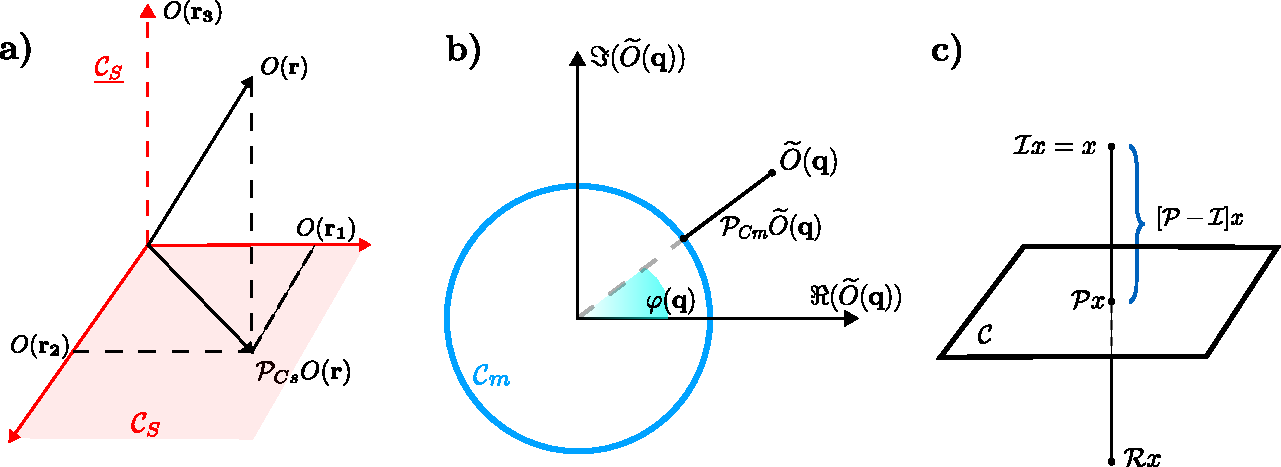
\includegraphics[width=\textwidth]{figures/Intro/projections.pdf}
    \caption{\textbf{a} Geometrical representation of the projection of the object onto the support constraint set.  
    \textbf{b} Geometrical representation of the projection of the object onto the Fourier modulus constraint set.
    \textbf{c} Geometrical representation of the identity, projector and reflector operators. Inspired by \cite{marchesini_unified_2007}}
    \label{fig:projections}
\end{figure}

In our case we have that the projector onto $C_s$ applied to the object sets to zero the values outside the support and does not 
alter the values inside: 
\begin{equation}
    \mathcal{P}_{Cs}(O(\mathbf{r})) = 
    \begin{cases}
        O(\mathbf{r}), & \mathbf{r} \in \mathcal{S} \\
        0,  &  \mathbf{r} \notin \mathcal{S}
     \end{cases}
\end{equation}

On the other hand the projector onto $C_m$ applied to the object replaces the modulus of its Fourier transform with the 
squared root of the measured intensity $m = \sqrt{I(\mathbf{q})}$. 
\begin{equation}
    \mathcal{P}_{Cm}(\widehat{O}(\mathbf{q})) = \mathcal{P}_{Cm}(A(q)e^{i\varphi(q)}) = \sqrt{I(\mathbf{q})}e^{i\varphi(q)}
    \label{eq:modulus_projection}
\end{equation}

This step forces the modulus of the Fourier transform of the object at the iteration $k$ to be exactly the measured magnitude.  

Since $\mathcal{P}_{Cm}$ and $\mathcal{P}_{Cs}$ operate in two conjugate spaces (direct-reciprocal), when used in sequence 
a direct or inverse Fourier transform is implied in between. The symbol will be omitted to simplify the notation. 

At this point we have all the necessary ingredients to introduce the three main AP algorithms used for BCDI PR. 

\subsection{Error Reduction (ER)}

If we consider as a starting point the object $O^0(\mathbf{r}) = \mathcal{F}^{-1}\{ \sqrt{I(\mathbf{q})}e^{i\varphi^0(\mathbf{q})}\}$, obtained by 
the inverse Fourier transform of the squared root of the measured intensity with a random complex phase array $\varphi^0(\mathbf{q})$, 
we can express the object at the $k-th$ iteration of the \textit{Error Reduction} (ER) algorithm as: 

\begin{equation}
    O^{k+1}(\mathbf{r}) = \mathcal{P}_{Cm}\mathcal{P}_{Cs}(O^{k}(\mathbf{r}))
    \label{eq:ER}
\end{equation}

This is the simplest and most intuitive AP algorithm as it only projects back and forth the object between the two sets. 
Although it guarantees linear convergence, ER is not optimal since it only converges to the nearest local minimum, and it is unable 
to escape it. For this reason in typical BCDI it is used to at the end of the PR, when the current estimate is close enough 
to the final solution.
Additionally, one can define the magnitude error functional $\varepsilon_m(O)$ as: 
\begin{equation}
    \varepsilon_m(O) = || \mathcal{P}_{Cm}(O)  - O ||_{L2} 
    \label{eq:error_magnitude}
\end{equation}
i.e. the Euclidean distance between the current estimate $O$ and its projection onto the Fourier modulus constraint set. 
Differentiating this functional with respect to $O$ yields the gradient $\nabla \varepsilon_m(O)$, which points in the 
direction that reduces the Fourier magnitude mismatch, or in other words, the natural descent direction of the error.
If this gradient is further restricted to the support constraint set, one obtains a 
\textit{projected gradient-descent step} $\nabla_s \varepsilon_m(O)$ which is the part of the descent direction that 
lies inside the feasible object region.

Marchesini shows that the ER step can thus be rewritten as:
\begin{equation}
    O^{k+1}(\mathbf{r}) = \mathcal{P}_{Cs}(O^{k}(\mathbf{r})) - \frac{1}{2}\nabla_s \varepsilon^{2}_m(O^{k}(\mathbf{r}))
    \label{eq:ER_gradient}
\end{equation}

which makes explicit the equivalence between ER and steepest descent projected onto the support constraint set, with 
a fixed step size of $1/2$.

\subsection{Hybrid Input-Output (HIO)}
The Hybrid-Input Output (HIO) algorithm introduces a nonlinear feedback that is essential to escape local minima. 
Specifically, we can express the object at the $k-th$ iteration as: 

\begin{equation}
    O^{k+1}(\mathbf{r}) = 
    \begin{cases}
        \mathcal{P}_{Cm}(O^{k}(\mathbf{r})), &   \mathbf{r} \in \mathcal{S} \\
        (\mathcal{I} -\beta\mathcal{P}_{Cm})(O^{k}(\mathbf{r})),  & \mathbf{r} \notin \mathcal{S}
     \end{cases}
     \label{eq:HIO}
\end{equation}

where $\beta$ is a positive hyperparameter with value typically around $0.9$.
Inside the support, the estimate is replaced by its Fourier-modulus projection. Outside the support, instead of being 
set to zero (as in ER), the estimate is updated with a feedback term proportional to the modulus projection. 
This subtraction, which can in principle yield negative values as well, prevents stagnation and allows the algorithm 
to explore solutions that are consistent with both the support and modulus constraints.
However, it is worth mentioning that due to the nonlinear feedback outside the support, HIO does not converge to local 
minima but rather towards \textit{saddle} points of the error functional. For this reason HIO is used in
combination with ER: HIO drives the reconstruction away from traps by oscillating near saddle points, and ER then 
provides stable convergence once the estimate is close to a true solution. 

\begin{figure}[H]
    \centering
    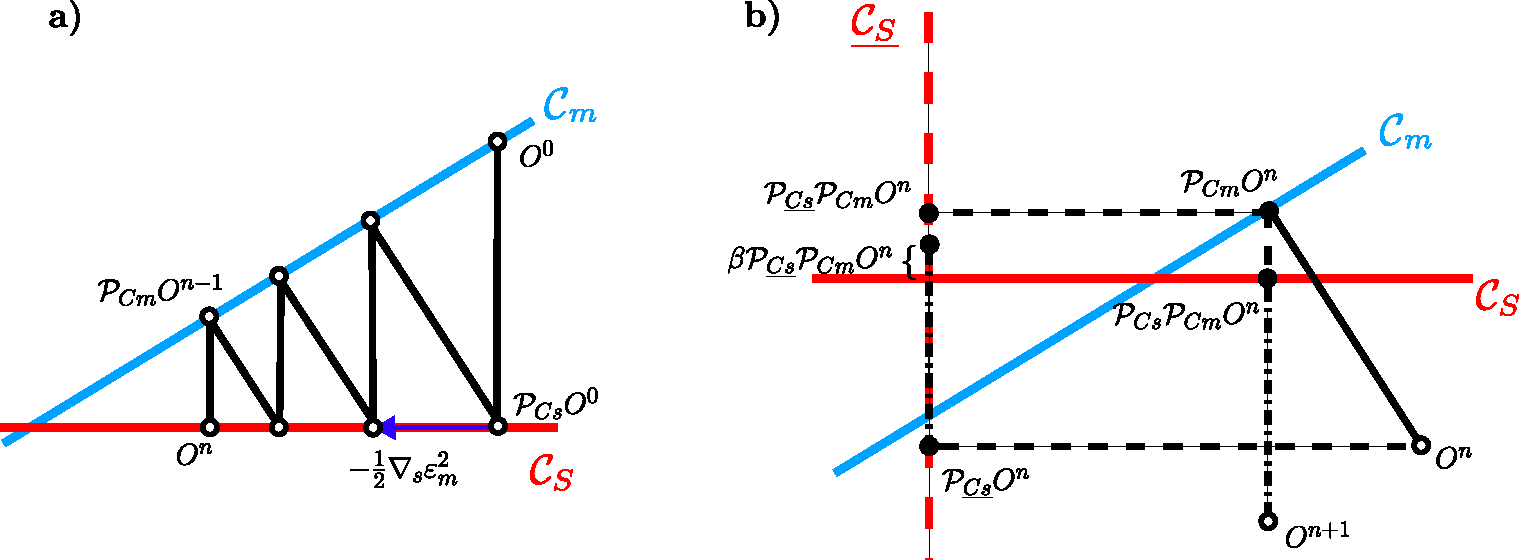
\includegraphics[width=\textwidth]{figures/Intro/ER_HIO.pdf}
    \caption{\textbf{a} Geometrical representation of the ER algorithm. Red and blue lines represent the support and 
    Fourier modulus constraint sets respectively. The alternated projections on the two constraint sets drive eventually 
    the estimate to the intersection. This is however only valid in a local subset of the solution space, where the -
    generally non-convex - modulus constraint set is convex and . 
    \textbf{b} Geometrical representation of the HIO algorithm .
     Inspired by \cite{marchesini_unified_2007}}
    \label{fig:projections}
\end{figure}


\subsection{Relaxed Averaged Alternating Reflections (RAAR)}
Another AP algorithm typically used in CDI is the Relaxed Averaged Alternating Reflections (RAAR) developed by Luke 
in 2004 \cite{Luke_2004}. According to this algorithm the object at the $k-th$ iteration is: 
\begin{equation}
    O^{k+1}(\mathbf{r}) =\beta\frac{1}{2}(\mathcal{R}_{Cs}\mathcal{R}_{Cm} + \mathcal{I})(O^{k}(\mathbf{r})) + (1-\beta)\mathcal{P}_{Cm}(O^{k}(\mathbf{r}))
    \label{eq:RAAR}
\end{equation}

where $\beta \in [0,1]$. 
Eq.\ref{eq:RAAR} can be split into two terms. The first term, known as Average Alternating Reflection (ARR) \cite{AAR_2004} 
acts like an average of the current estimate and its reflection across both constraints sets. The alternated reflections search 
for the intersection of the two sets, which is a fixed point of the problem, while exploring more broadly the solution 
space as they do not project directly on the constraint sets. The second term is a relaxation term that 
projects the current estimate on the modulus set, like in the HIO and ER. 

In short, one could see the RAAR as a controlled (through $\beta$) balance of exploration and stability. 

\subsection{Support update}
At this point of the discussion we should ask ourselves how do we know the \textit{support} function $\mathcal{S}$
required in all PR algorithms? We have said that in the BCDI case we typically do not know the shape of the particle 
a priori, and should therefore come as product of the PR.  
It is common practice in iterative phase retrieval to estimate the initial support 
from the object's autocorrelation,
\begin{equation}
    A(\mathbf{r}) = \mathcal{F}^{-1}\{ I(\mathbf{q}) \}
\end{equation}

However, the autocorrelation extends over a region roughly twice the linear size of the true object (see Fig.). 

An important step forward was introduced by Marchesini in 2003~\cite{Marchesini_shrinkwrap}: 
the \textit{shrinkwrap algorithm}, which adaptively refines the support during reconstruction. 
After a given number of phase retrieval iterations, the modulus of the current object estimate is 
convolved with a Gaussian kernel and subsequently thresholded (typically at $\sim$20\% of the maximum value), 
yielding a binary mask that defines the updated support. 

This adaptive support refinement was shown to significantly improve convergence and reconstruction quality 
in many experimental cases (depending on the signal-to-noise ratio and choice of threshold), and it is now a 
standard component of BCDI phase retrieval pipelines.\\

Later in the text we will refer to ``standard iterative algorithms'' or ``conventional PR'' as the combination of AP 
algorithms and support updates like Shrinkwrap. 

% \section{Gradient descent based methods}

% Up to now, most of the practical cases of PR for CDI rely on AP algorithms because of the limited computing time necessary 
% for the Fourier transforms and the projector/reflectors operators. 
% Another way of approaching the Phase Problem is via the more classical gradient descent methods. 
% In this case the Phase Problem is formulated as a minimization problem in a specific metric.
% For instance in $L_2$ norm metric it can be written as:

% \begin{equation}
%     O^{\ast}(\mathbf{r})
%     = \argmin_{O \in \mathbb{C}^N}
%     \left\| \, \big| \mathcal{F}\{O\} \big| - \sqrt{I} \, \right\|_2^2 .
% \end{equation} 

% According to which it takes the form of a least-square minimization problem. 
 
% \subsection{Steepest descent}

% \subsection{Conjugate Gradient Methods}

% \section{High strain and local minima}

% \section{Conclusions}

% % CHAPTER 3 - BCDI-strain
% \chapter{BCDI with high-strain}
% \label{chap:bcdi_strain}
% In this Chapter the specific case of BCDI in presence of highly strained particle or large phase ranges will be introduced. 
In first place, some qualitative considerations will be made starting from Eq. \ref{eq:strain_fin3}, Eq.\ref{eq:strain_fin4} and 
Eq.\ref{eq:fourie_relation} regarding the effect of displacement fields on the resulting diffraction pattern. 

Secondly, the effect of Poisson noise in combination with strain will be discussed as well. 
Lastly, we will try to evaluate the complexity of the Phase Retrieval with the amount of strain inside the particle. 

\section{Strain and resolution}

% CHAPTER 3 - Convolutional Neural Networks
\chapter{Keynotes on Convolutional Neural Networks}
\label{chap:dl_theory}


In this chapter a short overview on the basic concepts of Convolutional Neural Networks (CNNs) will be given. 
The scope is to give the necessary background for the understanding of the structure and the motivations behind the 
Deep Learning (DL) models employed for the analysis of BCDI data, presented in the next chapters.  

For more comprehensive and exhaustive dissertations about Machine Learning (ML) and Artificial Neural Networks (ANNs)
the book of Goodfellow \cite{Goodfellow_2016} and the more recent from Prince \cite{prince2023understanding} are 
suggested to the reader. 

\section{Artificial Neural Networks (ANNs)}

ANNs is a type of machine learning algorithm inspired by the biological neuron structure. ANNs are generally composed of interconnected 
nodes where the signal is processed through operations with tunable parameters named weights 
and biases for multiplications and addition respectively. Important feature of each node is the \textit{activation function}, 
that introduces a non-linear operation and returns the node's output \cite{jagtap2022}. Several kinds of these 
activation functions exist and their use depends on the properties of each (bounds, derivatives, positivity, etc.) 
\cite{kunc2024}. In the following chapters the modified rectifying linear unit, known as LeakyReLU \cite{Maas2013RectifierNI}, 
and the sigmoid, also known as logistic, function will be used. Neurons are generally organized into \textit{layers} and 
are connected between neurons of other layers. In \textit{feed-forward} neural networks the information flows from the 
input layer to the output layer with forward connections only.
In other neural networks, like \textit{recurrent} ones, the connections are also designed backwards. 

\begin{figure}[H]
    \centering
    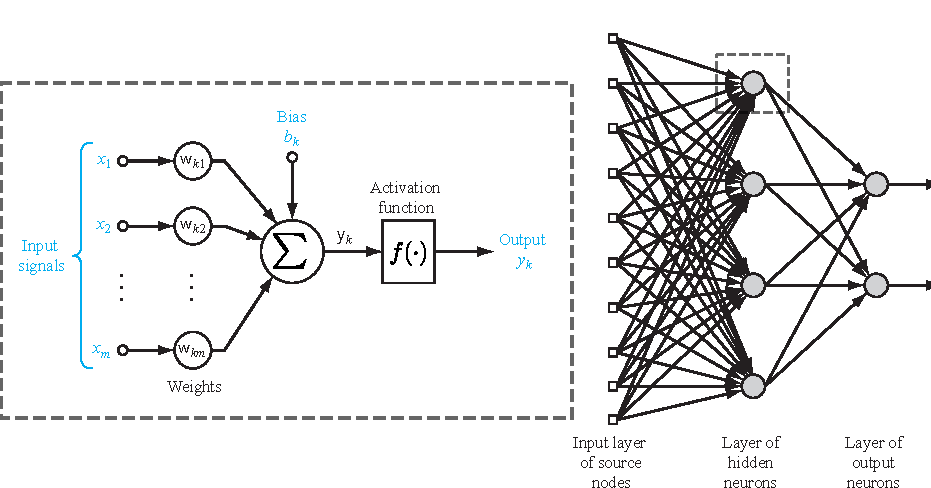
\includegraphics[width=\textwidth]{figures/Intro/neuron2.pdf}
    \caption{\textbf{Schematic of an artificial neuron and a neural network.} On the left, a series of input signals 
    $x_i$ are multiplied by the tunable weight $w_{k}$ and summed together with the tunable bias $b_k$ relative to 
    the $k$-th neuron. The output is then passed through the activation function $f$ which produce an output $y_k$ 
    which is a non-linear combination of the inputs. On the right, the feed-forward network composed 
    of two \textit{hidden} layers of artificial neurons processing the ten units long vector $x$ and returning a 
    binary output. Networks of this type are said to be \textit{fully connected} as each input component, or 
    node's output is processed by all neurons. Adapted from \cite{haykin2009neural}}
    \label{fig:neuron}
\end{figure}

\subsection{Neural networks as universal approximators}

The use of non-linear functions is found to be fundamental for the powerful analytical and statistical properties of ANNs, 
which have been progressively 
established over the years. It was shown \cite{Cybenko1989, Hornik_1989, Leshno_1993} that ANNs with appropriate 
activation functions and sufficient parameters can approximate \textit{any} continuous function on a compact domain to arbitrary 
accuracy (\textit{universal approximation theorems}). Later the proof has been extended to deep convolutional neural 
networks as well \cite{UniversalityCNN_2020}.

Formally, we can consider $\mathcal{X}$ as the set of all events belonging to the same statistical distribution and 
$\mathcal{Y}$ similarly. We also assume that an unknown mapping $\mathcal{M}$ between an input $x \in \mathcal{X}$ and the output 
$y = \mathcal{M}(x)$ exists. At this point, the goal of the ANNs is to be the closest approximation of $\mathcal{M}$.
Typically, this implies seeking the combination of parameters $\theta_k = (w_k, b_k)$ of the neural network $\mathcal{N}_{\theta}$ 
such that $\mathcal{N}_{\theta} \approx \mathcal{M}$

\textbf{How is this mapping found?} The core idea is known as Empirical Risk Minimization and states that 
when the $\theta_k$ are adjusted to fit a sufficiently large dataset consisting of samples drawn from an underlying distribution, 
the function being approximated reflects the statistical relationships encoded in that distribution \cite{Hornik_1990}.
By the Law of Large Numbers, the empirical distribution observed in the \textit{training set} converges to the true 
distribution as the sample size grows, and thus the empirical risk minimized during training approaches the true 
risk. This statistical foundation explains why ANNs are able to generalize to new, unseen data drawn from the 
same population. 

It is therefore sufficient to have a large but finite number of samples representative of both the sets $\mathcal{X}$ 
and $\mathcal{Y}$ to approximate $\mathcal{M}$. This powerful statistical property underlies the concept of \textit{supervised} 
training of ANNs. 

More formally, one can consider having a limited set of $N$ examples $(x_1,y_1 = \mathcal{M}(x_1)), ..., (x_N, y_N = \mathcal{M}(x_N))$ 
which we call \textit{training set} $\mathcal{T}$. Here, each $x_i$ is an input instance and $y_i$ the 
corresponding ground truth transformation operated by $\mathcal{M}$. We can now introduce a non-negative scalar 
real-valued \textit{loss function} $L(\hat{y},y )$ which measures the difference between the ground truth $y$ and the 
output of the neural network $\hat{y} = \mathcal{N}_\theta (x)$ for each element of the training set.

It follows that the best approximation of the mapping $ \mathcal{N}_\theta^{\mathcal{T}} \approx \mathcal{M}^{\mathcal{T}}$ is 
obtained when the score of the loss function averaged across the number of training samples is lowest.
The problem of approximating the mapping between the input and ground truth in the training set is then formulated as 
minimization problem of the type: 

\begin{equation}
    \hat{\theta}_{\mathcal T}
    = \arg\min_{\theta} 
    \left\{ \frac{1}{N} \sum_{i=1}^N 
    L\!\left(y_i, \mathcal{N}_{\theta}^{\mathcal{T}}(x_i)\right) 
    \right\}
\end{equation}

For a sufficiently large $N$ the $\hat{\theta}_{\mathcal T} \approx \hat{\theta}$ valid for the whole statistical distribution. 
The size of $N$ needed to approach the true mapping depends obviously on the complexity of the mapping and on the 
complexity of the minimization task. While the first is inherent to the problem, the second can be engineered with 
the choice of a metric for which the loss function minimization is easier. This will be clear in Chapter \ref{chap:phase_retrieval}
where different loss functions are tested. In the same way, the network design can impact the facility with which the 
ANN converges to the approximation of the desired mapping. In these regards, the use of multiple intermediate layers 
of neurons (\textit{hidden layers}) was shown to strongly improve the ability of the NN to fit more complex functions
(see \cite{prince2023understanding} - Chapter 4.5). 
For this reason these network called \textit{deep} have taken over \textit{shallow} ones. Another example, briefly 
discussed in the next section, is given by Convolutional Neural Networks (CNNs), a type of ANN suited for natural image 
processing.  

Moreover, in cases in which one does not have a training set composed of input - ground truth pairs, but instead 
incorporates prior knowledge into the model architecture or the loss function, the training is said to be 
\textit{unsupervised}. This approach has not been explored in the context of this PhD. 

\subsection{Gradient Descent}

At this point another question may arise: \textbf{How are do we solve the minimization problem?}
The most straightforward manner to solve a minimization problem is with gradient descent. This implies an iterative process 
in which at each iteration the derivatives of the loss function with respect to each parameter $\theta$ are calculated, 
and each parameter is updated correspondingly. 

\begin{equation}
    \theta^{t+1}
    = \theta^{t} - \eta \nabla_{\theta} \left[ \frac{1}{N} \sum_{i=1}^N 
    L\!\left(y_i, \mathcal{N}_\theta(x_i)\right) \right]
    \label{eq:steepest_gd}
\end{equation}

Where $\eta$ is the \textit{learning rate} that is given as external parameter (\textit{hyperparameter}) to the model. 
Eq.\ref{eq:steepest_gd} implements the steepest gradient descent. However, in most machine learning optimizers a variant 
of this algorithm is computed. Namely, the gradients are calculated for sub-set, often called \textit{mini-batch} of the 
whole training set. During the training, within each \textit{epoch} as many mini-batches as needed to make the full 
dataset are minimized in series. This approach, called \textit{stochastic} gradient descent (SGD), is less expensive 
in terms of memory and offers well established convergence properties that outperform classical steepest descent methods 
\cite{Zhao2021_sgd}. In fact, the ``noise'' affecting the updates induced by the minimization of a small sub-set can be beneficial 
for escaping saddle points which may trap the search. 
In the years, different variants of SGD have been proposed. The ``momentum'' calculation \cite{Polyak1964}, 
that keeps track of the magnitude and direction of the updates and determines the next update as a linear combination 
of the gradient and the previous update, was first applied to SGD \cite{Backpro_1986}. Later, adaptive approaches 
have aimed at tuning the learning rate differently for each parameter (AdaGrad \cite{Adagrad}, ADAM \cite{ADAM}).
Later in the text, the DL models employed have adopted ADAM optimizer. 
It is worth mentioning that, though the most widely used, gradient descent approaches are not the only strategies that 
have been explored to minimize the loss function. Evolutionary algorithms inspired by natural selection mechanisms and 
tensor optimization techniques developed in the quantum-many body field have been employed as well \cite{EA_1999, DMRG_Stoudenmire}.

\begin{figure}[H]
    \centering
    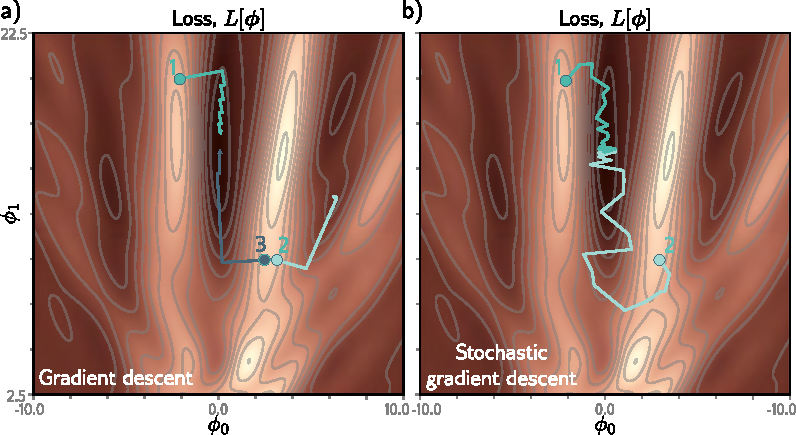
\includegraphics[width=\textwidth]{figures/Intro/sgd.pdf}
    \caption{\textbf{Gradient descent and Stochastic gradient descent. a)} Depicts the trajectory of the error score in 
     a 2D loss function in case of gradient descent with line search from three different initializations. The 
     algorithm converges to the global minimum when it starts from points 1 and 3 while it fails when it starts from 
     point 2, located outside the valley of the global minimum. \textbf{b)} The same experiment solved with stochastic 
     gradient descent achieves good convergence also when initialized from point 2. Indeed, the ``noise'' introduced 
     by the mini-batches drives the updates outside the wrong valley and allow the convergence to the global minimum. 
    Adapted from \cite{prince2023understanding}}
    \label{fig:sgd}
\end{figure}

\subsection{Backpropagation and automatic differentiation}

At this stage, a crucial question arises: \textbf{how can SGD be efficiently implemented in practice?}
ANNs often involve millions or even billions of parameters $\theta$, thus computing exact derivatives with respect to 
such a large number of variables, for every batch and across multiple epochs, requires highly optimized algorithms 
and hardware acceleration.
Indeed, the practical feasibility of training neural networks was significantly advanced by the seminal work of Rumelhart, 
Hinton, and Williams in 1986 \cite{Backpro_1986}, which introduced the efficient \textit{back-propagation} technique that made 
large-scale training computationally tractable.

Back-propagation bases its principles on the fundamental \textit{chain rule} proposed by Leibniz in 1676 to calculate 
derivatives of function compositions. In fact, a ANNs can be seen as a composition of functions (the layers) in which 
at each stage the layer $i$-th processes the output of the layer $(i-1)$-th. Formally, one can write: 

\begin{equation}
    \mathcal{N}_{\theta} = f_\theta^{(L)} \circ f_\theta^{(L-1)} \circ ... \circ f_\theta^{0}
    \label{eq:composition}
\end{equation}

Where $f_\theta^{(L)}$ is the function representing the $L$-th layer of neurons of parameters $\theta$. The gradient 
of the loss function with respect to the parameters is therefore expressed, according to the chain rule as: 

\begin{equation}
    \nabla_{\theta^{(l)}} L  = \frac{\partial{(L)}}{\partial{f^{(L)}}} \cdot \frac{\partial{f^{(L)}}}{\partial{f^{(L-1)}}} 
    \cdot ... \cdot \frac{\partial{f^{(l)}}}{\partial{\theta^{(l)}}}
    \label{eq:chain_rule}
\end{equation}

This method decomposes the calculation of the full gradient into a sequence of smaller, local derivatives, each 
associated with the intermediate states of the network. During the forward pass, the activations and local 
Jacobians are computed and stored in memory, a process sometimes referred to as \textit{forward accumulation}. 
These stored quantities are then systematically reused during the backward pass to propagate gradients from the 
output layer back through the network parameters. This reuse of intermediate computations is what makes the 
algorithm highly efficient, and it is from this backward flow of gradients that the name \textit{back-propagation} 
originates.  

In modern machine learning frameworks such as PyTorch \cite{paszke2019pytorch} and TensorFlow 
\cite{abadi2016tensorflow}, back-propagation is implemented through the construction of a 
\textit{computational graph}. Each node in the graph represents an operation, while edges encode the dependencies 
between operations. Once the forward pass has been executed, this graph allows the backward pass to be automatically 
derived and executed, efficiently parallelized across GPUs or TPUs. In fact, back-propagation is a specific instance 
of a more general family of techniques known as \textit{automatic differentiation} (or \textit{algorithmic 
differentiation}) (AD) \cite{Griewank2000EvaluatingD, baydin2018}, and more precisely corresponds to 
\textit{reverse-mode automatic differentiation}. This connection highlights that back-propagation is not 
unique to neural networks, but rather belongs to rigorous and general framework for computing exact 
derivatives of functions defined by computer programs.  

% It is useful to contrast automatic differentiation with two other approaches for computing derivatives. 
% \textit{Symbolic differentiation}, as implemented for instance in computer algebra systems, manipulates expressions 
% analytically but suffers from expression swell and is not well suited for large computational graphs. 
% \textit{Numerical differentiation}, based on finite-difference approximations, is conceptually simple but prone to 
% numerical instability and scales poorly with the number of parameters. In contrast, automatic differentiation 
% combines the exactness of symbolic methods with the efficiency of numerical approaches, making it particularly 
% well suited for large-scale models such as neural networks.  

\begin{figure}[H]
    \centering
    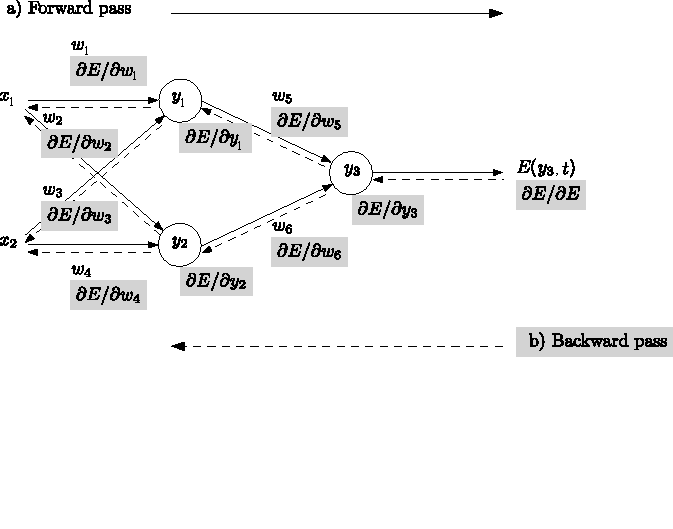
\includegraphics[width=\textwidth]{figures/Intro/backpro.pdf}
    \caption{\textbf{Schematic of Back-propagation on computational graph. a)} The training inputs $x_i$ are processed 
    in the forward pass by the network that produces intermediate states $y_{1,2}$ using weights $w_i$, and the final 
    output $y_3$. \textbf{b)} The error $E$ computed between the output and the estimate $t$ is propagated backward 
    and the gradients with respect to the weights $\nabla_{w_i} E = (\frac{\partial{E}}{\partial{w_1}},..., \frac{\partial{E}}{\partial{w_6}})$
    are obtained from the chain rule of derivatives. Adapted from \cite{baydin2018}}
    \label{fig:sgd}
\end{figure}

\newpage

\section{Convolutional Neural Networks (CNNs)}

It was anticipated earlier in the Chapter that the network design can strongly impact the learning of the mapping 
$\mathcal{M}$. In the specific case in which $\mathcal{X}, \mathcal{Y}$ represent sets of natural images, neural 
networks with layers employing convolution operations have shown to outperform fully connected ones \cite{Fukushima1982,LeCun1989Handwritten, LeCun1989Backpropagation}. 
The reasons behind the success of convolutions are intuitively explained as follows: 

\begin{itemize}

    \item Images are inherently high-dimensional, as they are defined on 2D or 3D grids. As a result, the number of 
    parameters required to connect each pixel in a fully connected neural network grows rapidly and soon becomes 
    intractable. Convolutional layers address this issue by employing a \textit{kernel}: a small trainable filter 
    that is convolved with the input image or intermediate feature maps. This mechanism enables weight reuse across spatial 
    locations, drastically reducing the number of trainable parameters, a property commonly referred to as 
    \textit{parameter sharing}. Furthermore, the localized receptive field of the kernel induces a form of structured 
    sparsity, effectively regularizing the model by constraining the mapping to be approximated using compact, spatially 
    coherent information.

    \item  In images, spatially adjacent pixels are typically correlated, while uncorrelated variations are often 
    attributable to noise. Fully connected layers process each pixel independently, requiring the network to learn 
    spatial dependencies solely through training. Convolutional layers, in contrast, explicitly exploit local spatial 
    correlations by aggregating information from neighboring pixels, thereby embedding structural priors into the 
    architecture. (see Fig. \ref{fig:conv})

    \item The image of a tree and another image of the same tree, translated require a different tuning of the
    weights in a fully-connected layer, although the interpretation of the image has not physically changed. 
    Learning a different parameter configuration for each different translation of the same object is highly inefficient. 
    On the contrary, an additional benefit of the parameter sharing in convolutional layers is the equivariance to 
    translation that inherently optimize the learning. This property allows the output to respond to the input change 
    in the same way. Note that this equivariance is not valid for other geometrical transformations like rotation and 
    magnification.

\end{itemize} 

% motivation
We have seen in Chapter \ref{chap:bcdi} that BCDI data is in the form of 3D images in which peculiar spatial structures 
made of peaks and fringes are clearly visible, hence the natural choice of convolutional neural networks. Moreover, the 
tasks addressed in this PhD thesis, namely the gap-inpainting and the phase retrieval, are classified as inverse problems 
where the goal is to reconstruct missing or unmeasured information from incomplete observations. As highlighted in recent 
surveys and related works \cite{Review_CNN_2020, CNN_inverse2017}, CNNs are particularly well suited for these problems 
because they can learn powerful image priors from data, act as regularizers even without extensive training 
(as shown in the Deep Image Prior framework \cite{Ulyanov_2020}), and can be combined with physics-based models to 
enforce data consistency.

Let us present now the building blocks of a typical convolutional neural network.

\subsection{Convolutional layer}

The initialization of a convolutional layer in typical machine learning libraries involve the definition of: 
\begin{itemize}
    \item An integer number of kernels. This number corresponds to number of filters through which the input is 
    processed in a convolution operation. Each filter is normally associated to a different feature of the input 
    image that is extracted by the corresponding kernel. The output of the convolutional layer will 
    have an extra dimension (called \textit{channel}) with size corresponding to the number of filters.  

    \item The integer-valued size of the kernel. In 2D convolutions the kernel is a matrix and similarly 
    extended to a 3D tensor for three-dimensional inputs. It controls the scale of the features that the convolutional 
    layer can ``see''. Small kernels highlight small features and vice-versa.

    \item The padding parameter which handles the convolution at the borders of the image, where the kernel would 
    otherwise extend beyond the available data. It determines whether the output feature map maintains the same spatial 
    dimensions as the input (``same'' padding) or is reduced in size (``valid'' padding).

    \item The stride parameter: This integer-valued parameter (matrix in 2D and tensor in 3D) indicates the lateral shift 
    that is applied to the kernel across the image. If greater than 1 some pixels/voxels are skipped resulting in a 
    sort of sub-sampling allowing to filter out some low-level features. 
    
    \item The dilation rate, which is another integer-valued parameter (matrix in 2D and tensor in 3D) that allows 
    to insert holes between consecutive elements of the kernel. In this way the actual size of the kernel is increased 
    by the dilation value, but the overall number of weights is unvaried. This enables to cover a larger area of the input 
    without increasing the number of trainable parameters.

\end{itemize}

Additional features of a typical convolutional layer include the addition of trainable biases and the initialization and 
regularization of the kernels and biases. Lastly, a non-linear activation is usually applied to the output of 
the convolutional layer. 

We mention here the existence of so-called \textit{transposed convolutions} which are sometimes used in CNNs. Here the 
conceptual difference is that instead of sliding the kernel over the input, is the input sliding over the kernel and 
performing the element-wise multiplication and summation. Transposed convolutions naturally produce an output that is larger 
than the input, because they reverse the spatial reduction of a standard convolution. For this reason, they are often used 
to replace explicit \textit{up-sampling} layers, which increase the spatial size through fixed interpolation (e.g. nearest-
neighbor or bilinear). Unlike standard interpolation, transposed convolutions perform a \textit{learned} up-sampling, 
where the network optimizes the kernel weights to reconstruct high-resolution features in a data-driven way. 

\begin{figure}[H]
    \centering
    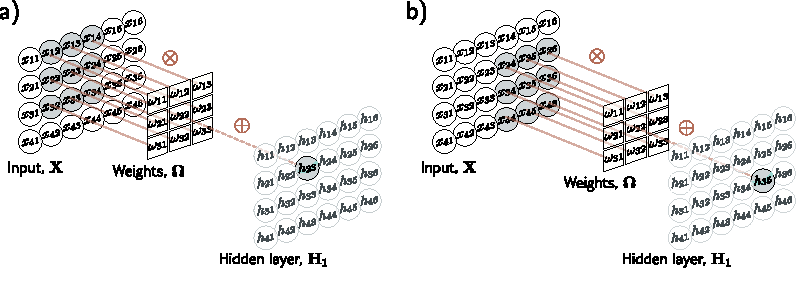
\includegraphics[width=\textwidth]{figures/Intro/conv.pdf}
    \caption{\textbf{Schematic of 2D convolutional layer:  a) } The convolution is operated over a region of the image 
    with same size as the kernel ($3 \times 3$). The result of the multiplication of each pixel value $(x_{12},...,x_{34})$ 
    times the weight $(w_{11},...,w_{33})$ is then summed into a scalar $h_{23}$. \textbf{b)} The same operation with 
    the same kernel is performed to a shifted window of the input image.
    Adapted from \cite{prince2023understanding}}
    \label{fig:conv}
\end{figure}

\subsection{Pooling Layer}

After the convolutional layer and the activation function, it is often the turn of a \textit{pooling} layer. For the 2D case, 
the output of the layer at specific location $i,j$ is the result of a filtering operation on the neighboring pixels 
of the input. For instance, the ``Max Pooling'' layer replaces a rectangular region of the input with its maximum value, 
thus retaining only the strongest activation within that area. In contrast, the ``Average Pooling'' layer 
assigns to the output pixel the mean value of all pixels in the corresponding region. 
The benefits deriving from the pooling layer are mostly twofold. First, the size of the output is reduced by a factor 
proportional to the area of the pooling window (or the volume in the 3D case), thus lowering the computational 
and memory cost of subsequent operations. Second, by condensing information into a smaller region, pooling encourages 
the network to learn representations that are more robust to small translations. For instance, with Max Pooling, 
a shift of the most activated pixel within the pooling window does not affect the output. This behavior can be 
interpreted as an implicit prior that biases the optimization towards translation-invariant approximations. 

\begin{figure}[H]
    \centering
    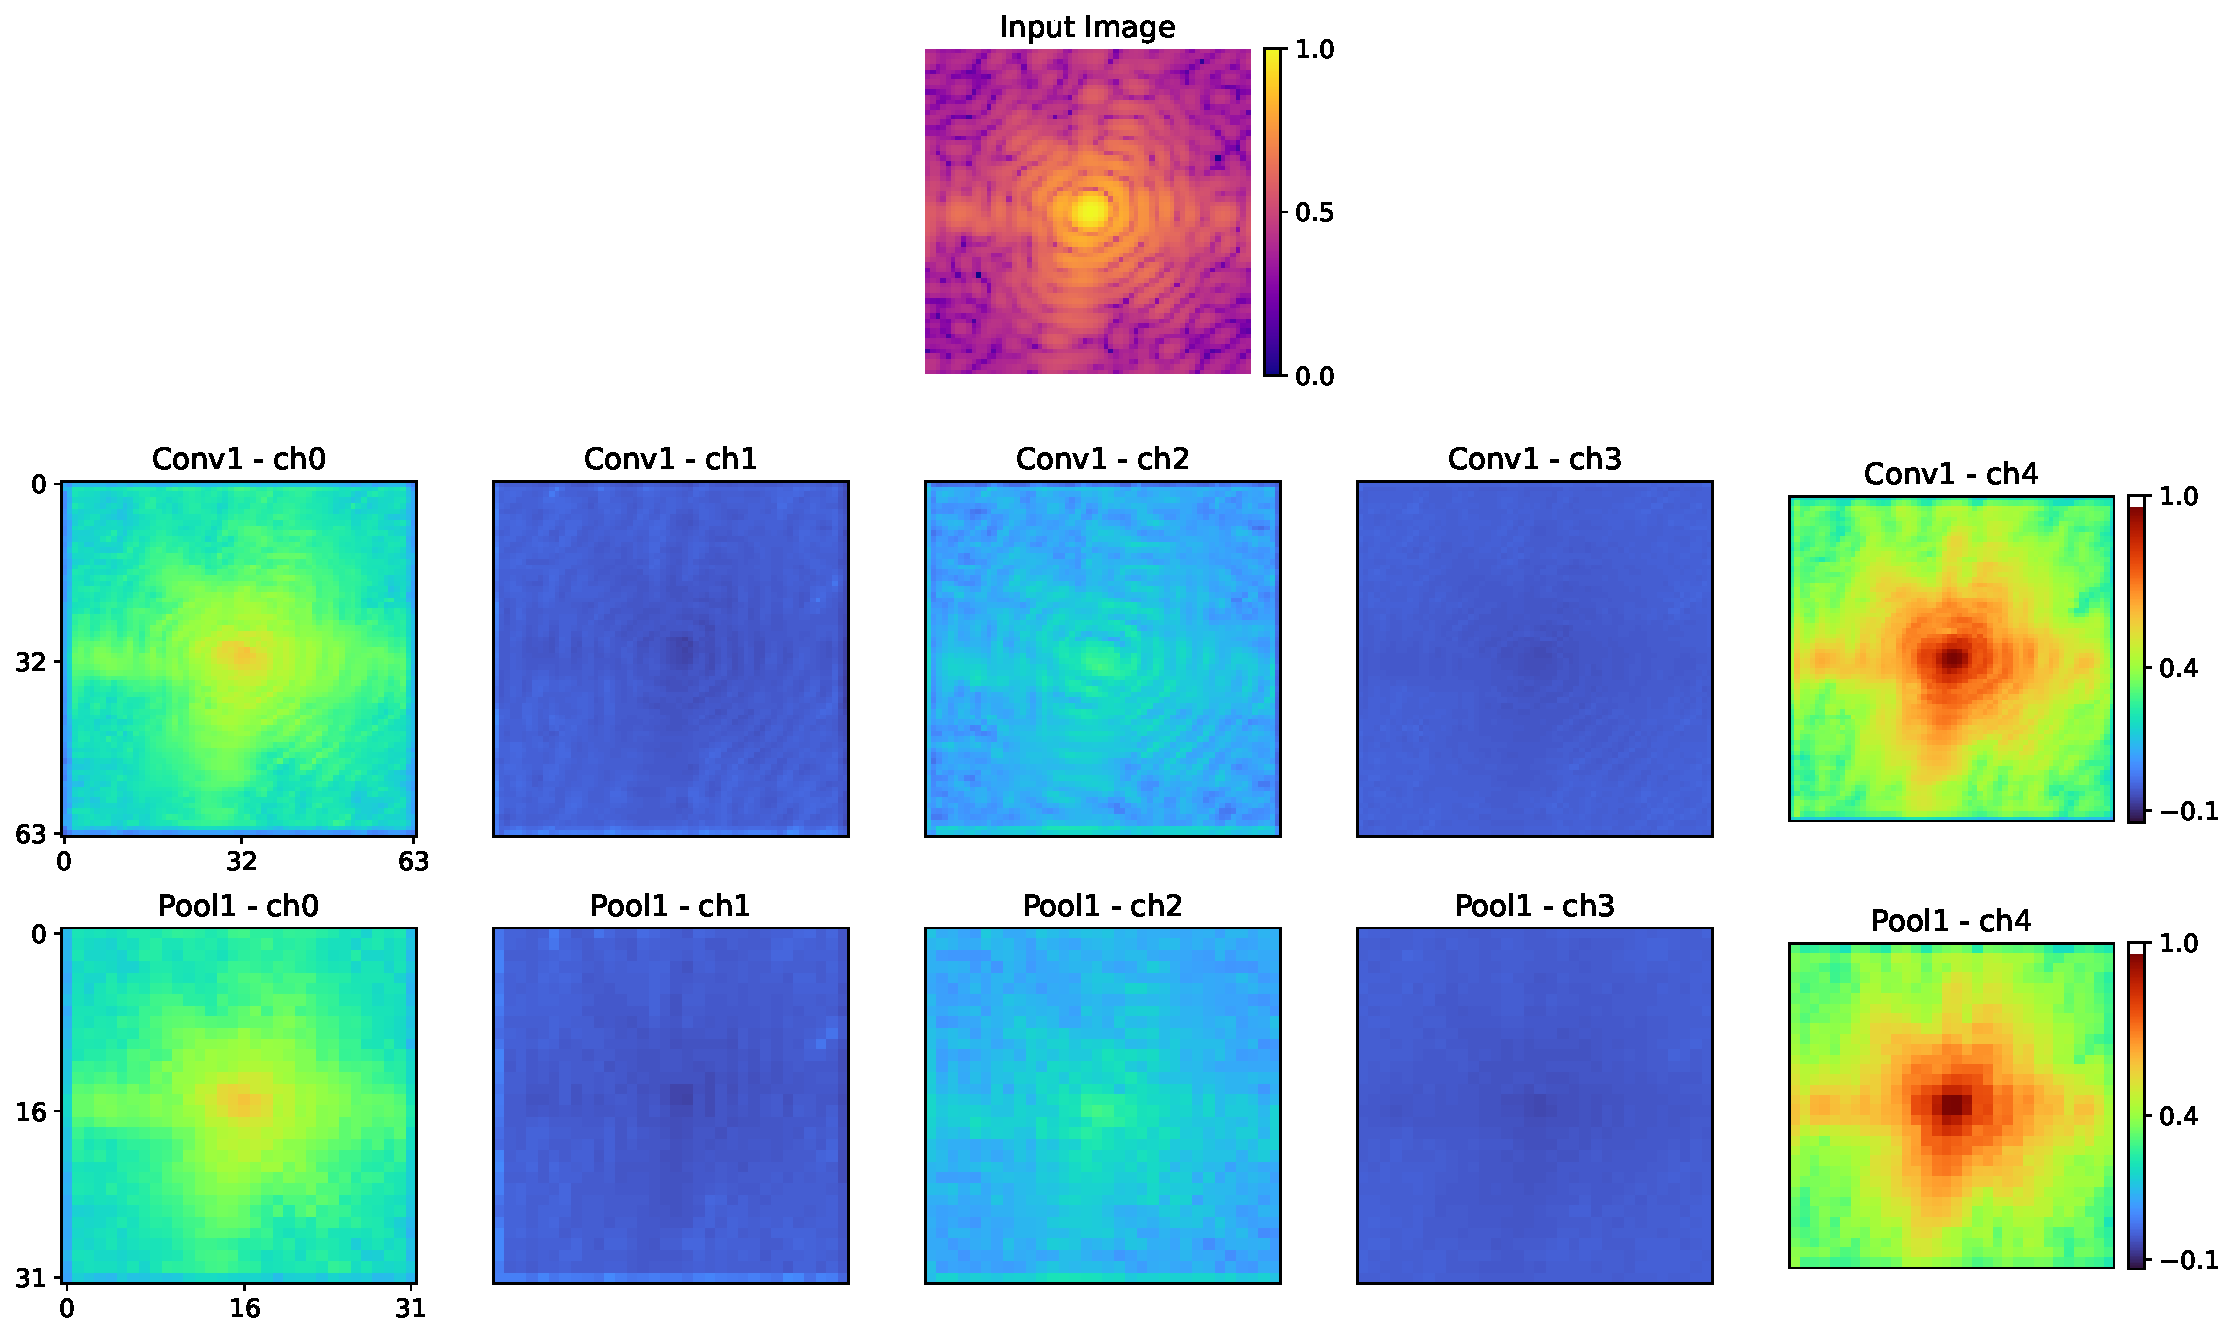
\includegraphics[width=\textwidth]{figures/Intro/conv_maxpool.pdf}
    \caption{\textbf{Example of Convolutional and Max pooling layers.} A simulated 2D BCDI pattern is input image 
    (first row) of the CNN model presented later in Chapter \ref{chap:phase_retrieval}, after the training. The output of the first 
    convolutional layer + LeakyReLU activation is displayed in the second row (first 5 channels) while the output of 
    the subsequent Max Pooling layer is displayed in the third row. Notice the similarity between the two rows despite 
    the halved size of Max Pooling output. This shows that it efficiently condenses the information into smaller sizes.
    % Moreover, one can notice how different channels extract different features, some of which (0 and 4 in this case) 
    % have larger amplitude, thus ``importance'' to the network.
    }
    \label{fig:convmaxpool}
\end{figure}


The typical convolutional block is therefore composed of these three layers (convolutional, activation, pooling). 
A sequential application of the convolutional blocks to a 2D or 3D input image is often called \textit{encoder} and 
can reduce the dimension of the 
feature map to as many 1D vectors as the number of filters of the last convolutional layer. During the training, this 
reduced representation of the input is more and more driven to capture the essential information in a lower-dimensional 
space. At this point, for \textit{classification} tasks the feature map is flattened into a single 1D vector 
being the input of a fully connected layer. The output of this last layer is then usually interpreted as the probability 
score for the input image to belong to a specific class. Among the milestone CNN models for classification, it is worth 
highlighting LeNet-5, introduced by LeCun in 1998 \cite{lecun1998gradient}, and AlexNet, which revolutionized the 
field by leveraging more efficient GPU-based training \cite{krizhevsky2012imagenet}.

In \textit{image generation} tasks, the lower-dimensional space, also called \textit{latent space} serves as input 
to a sequence of 
\textit{deconvolutional} blocks, where \textit{transposed} convolutions combined with activation functions 
progressively reconstruct the output image at the desired resolution. This sequence of deconvolutional layers 
is referred to as the \textit{decoder}, as it mirrors the encoder. In some architectures, up-sampling layers 
followed by standard convolutions are employed instead of transposed convolutions. Encoder-decoder architectures 
for image generation were first introduced by Hinton in 2006~\cite{hinton2006reducing}. This class of models is employed 
in a variety of tasks such as de-noising, image compression, inpainting, 
and segmentation. Although other types of models are also used for image generation, including Generative 
Adversarial Networks (GANs) \cite{goodfellow2014generativeadversarialnetworks} and Vision Transformers 
(ViTs) \cite{dosovitskiy2021imageworth16x16words}, in this manuscript we restrict our focus to 
encoder-decoder architectures.


\subsection{Skip connections}

Before concluding the chapter it is worth mentioning the concept of \textit{skip connections} (or \textit{residual 
connections}). 


% CHAPTER 4 - Deep Learning for Detector Gaps Inpainting
\chapter{Deep Learning for Detector Gaps Inpainting}
\label{chap:inpainting}

In this chapter the ``detectors' gaps problem'' in Bragg Coherent Diffraction Imaging and our approach to solve it
using Deep Learning are discussed. The main state-of-the-art measures are presented briefly and
the topic of image inpainting with Deep Learning is introduced. The focus will then shift to our works that led
eventually to the optimal ``Patching-based'' approach that can also be found in the published paper entitled
 \textit{``Patching-based deep learning model for the Inpainting of Bragg Coherent Diffraction patterns affected 
 by detectors' gaps''} (\url{https://doi.org/10.1107/S1600576724004163}). The chapter is closed with some analyses 
 of the performances of the DL models in a variety of simulated and experimental cases.  

\section{The ``Gap Problem''}\label{sec:gaps}

At time of writing, standard BCDI experiments employ pixelated photon counting detectors to acquire the diffraction
patterns. These detectors can guarantee high spatial resolution, noise-free counting and fast read-out times. Two examples 
of these devices, currently used at the ID01 beamline are the MAXIPIX and EIGER detectors \cite{ponchut_maxipix_2011, Eiger_Johnson_2014}.
These detectors are often built by tiling together several sensing chips in order to cover a larger area, and are
typically bonded to an Application-Specific Integrated Circuit (ASIC) using bump bonding. 
This implies the presence, in the overall sensing region, of vertical and/or horizontal stripes that are not sensitive
to the impinging radiation. The width of these lines varies depending on the device but normally does not exceed the equivalent 
of some tens of pixels. Specifically, the MAXIPIX detector, with sensing area of $516\times516$ pixels of 
$55\mu m\times55\mu m$, is composed of four modules separated by $220\mu m$ wide gaps (equivalent of 4 pixels). 

The EIGER detector instead has two types of larger gaps of 12 pixels and 38 pixels width.
The detector gaps problem does not affect BCDI only, but it is shared among other x-ray techniques that deal with single photon-counting
pixelated detectors and/or beamstops.
We have seen in chapter \ref{chp:intro} that during a BCDI scan the 2D images acquired by the detector are stacked to form
a 3D array. This leads these lines to become planes of missing signal in the dataset.
The problems arise when reconstructing the data affected by these gaps. In fact, these regions of non-physical zero intensity
deceive the Phase Retrieval algorithms inducing the presence of artifacts in the reconstructions\cite{carnis_towards_2019}.

\begin{figure}[h]
    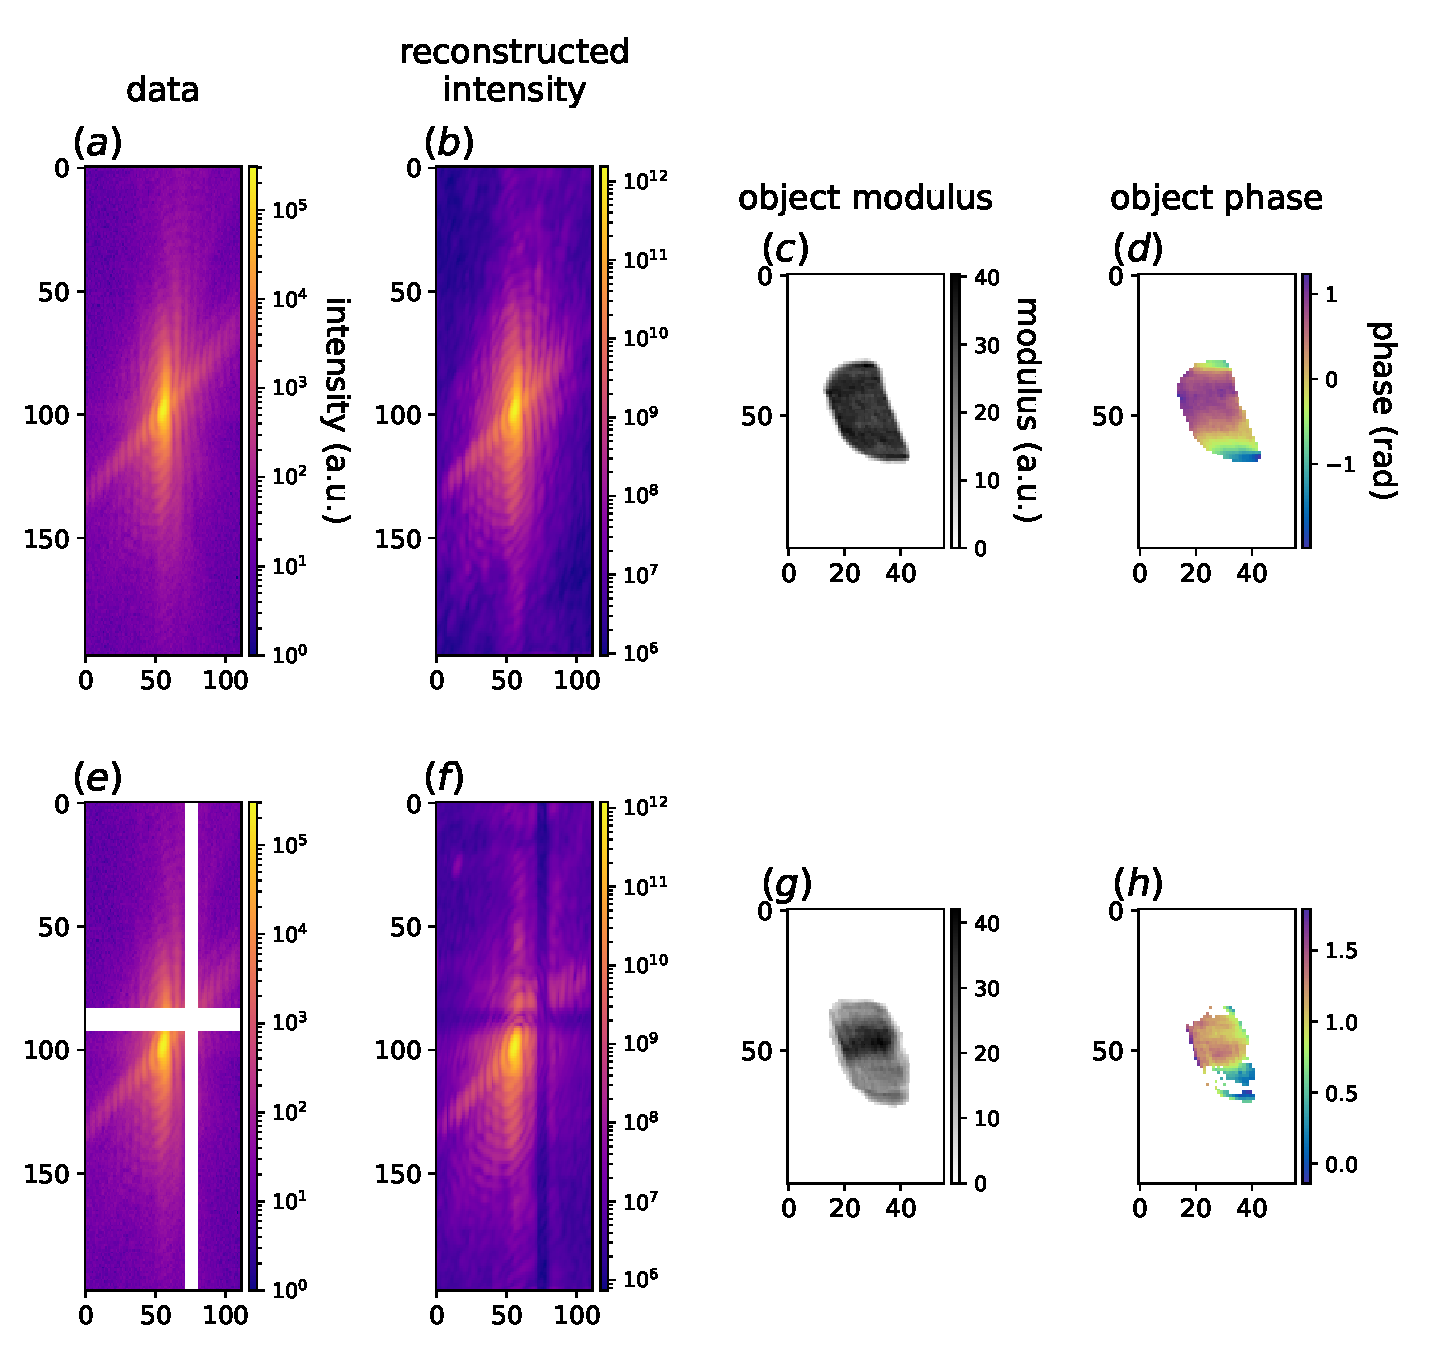
\includegraphics[width=\textwidth]{figures/Inpainting/gaps_intropdf.pdf}
    \caption{\textbf{Effect of detector gaps in BCDI reconstructions} 
    \textbf{(a)} The central xz slice of an experimental diffraction pattern. \textbf{(b)} The same slice of the diffracted
    intensity calculated from the retrieved object. \textbf{(c - d)} xz slice of the modulus and phase respectively of the particle
    obtained from the phasing of the gap-less dataset. \textbf{(e)} Same slice as in \textbf{(a)} with an artificially added
    9 pixel-wide, cross-shaped gaps to mimic the detector's ones. \textbf{(f)} The same slice of the diffracted
    intensity calculated from the retrieved object when not masking the gap regions. \textbf{(h - g)} xz slice of the modulus and phase respectively of the particle
    obtained from the phasing of the gap-affected dataset. The distortions caused by the gaps are evident. }
    \label{fig:gap_intro}
    \end{figure}


It follows that the reliability of the reconstructions in this case is 
compromised as the strain distribution can be deeply affected by the artifacts. A good practice during standard BCDI experiments
is to avoid the gaps by moving the detector if possible. However, this tends to be problematic for the case of high-resolution BCDI, 
i.e. when the diffraction pattern measurement extends to higher q-values, thus covering more than one sensing 
chip and necessarily crossing a gap region. Under these circumstances it becomes important to reduce the amount of
artifacts deriving from the gaps. 


\section{State of the art}\label{sec:InpStateArt}

Here we will discuss the current strategies employed to treat the detector gaps. As someone could argue, the simplest
yet not practical, solution would be to slightly move the detector sideways and acquire a second full scan with the
gap hiding a different region of the same Bragg peak, and then merge the two measurements into a single gap-less one. 
This would more than double the acquisition time making it, de facto, never an option during standard experiments. 

The PyNX software, routinely used for the BCDI phase retrieval at ID01, allows the user to define a mask of the gap 
regions and ignore those pixels during the execution. In this way the quality of the reconstruction improves, 
but one can still notice the presence of high-frequency oscillations appearing in both object's modulus and phase.
The origin of these artifacts can be found in the diffracted intensity calculated from the reconstructed particle as 
one can clearly see that the gap-regions is filled with nonphysically high intensity (see Fig. \ref{fig:gap_intro_mask})

\begin{figure}[h]
    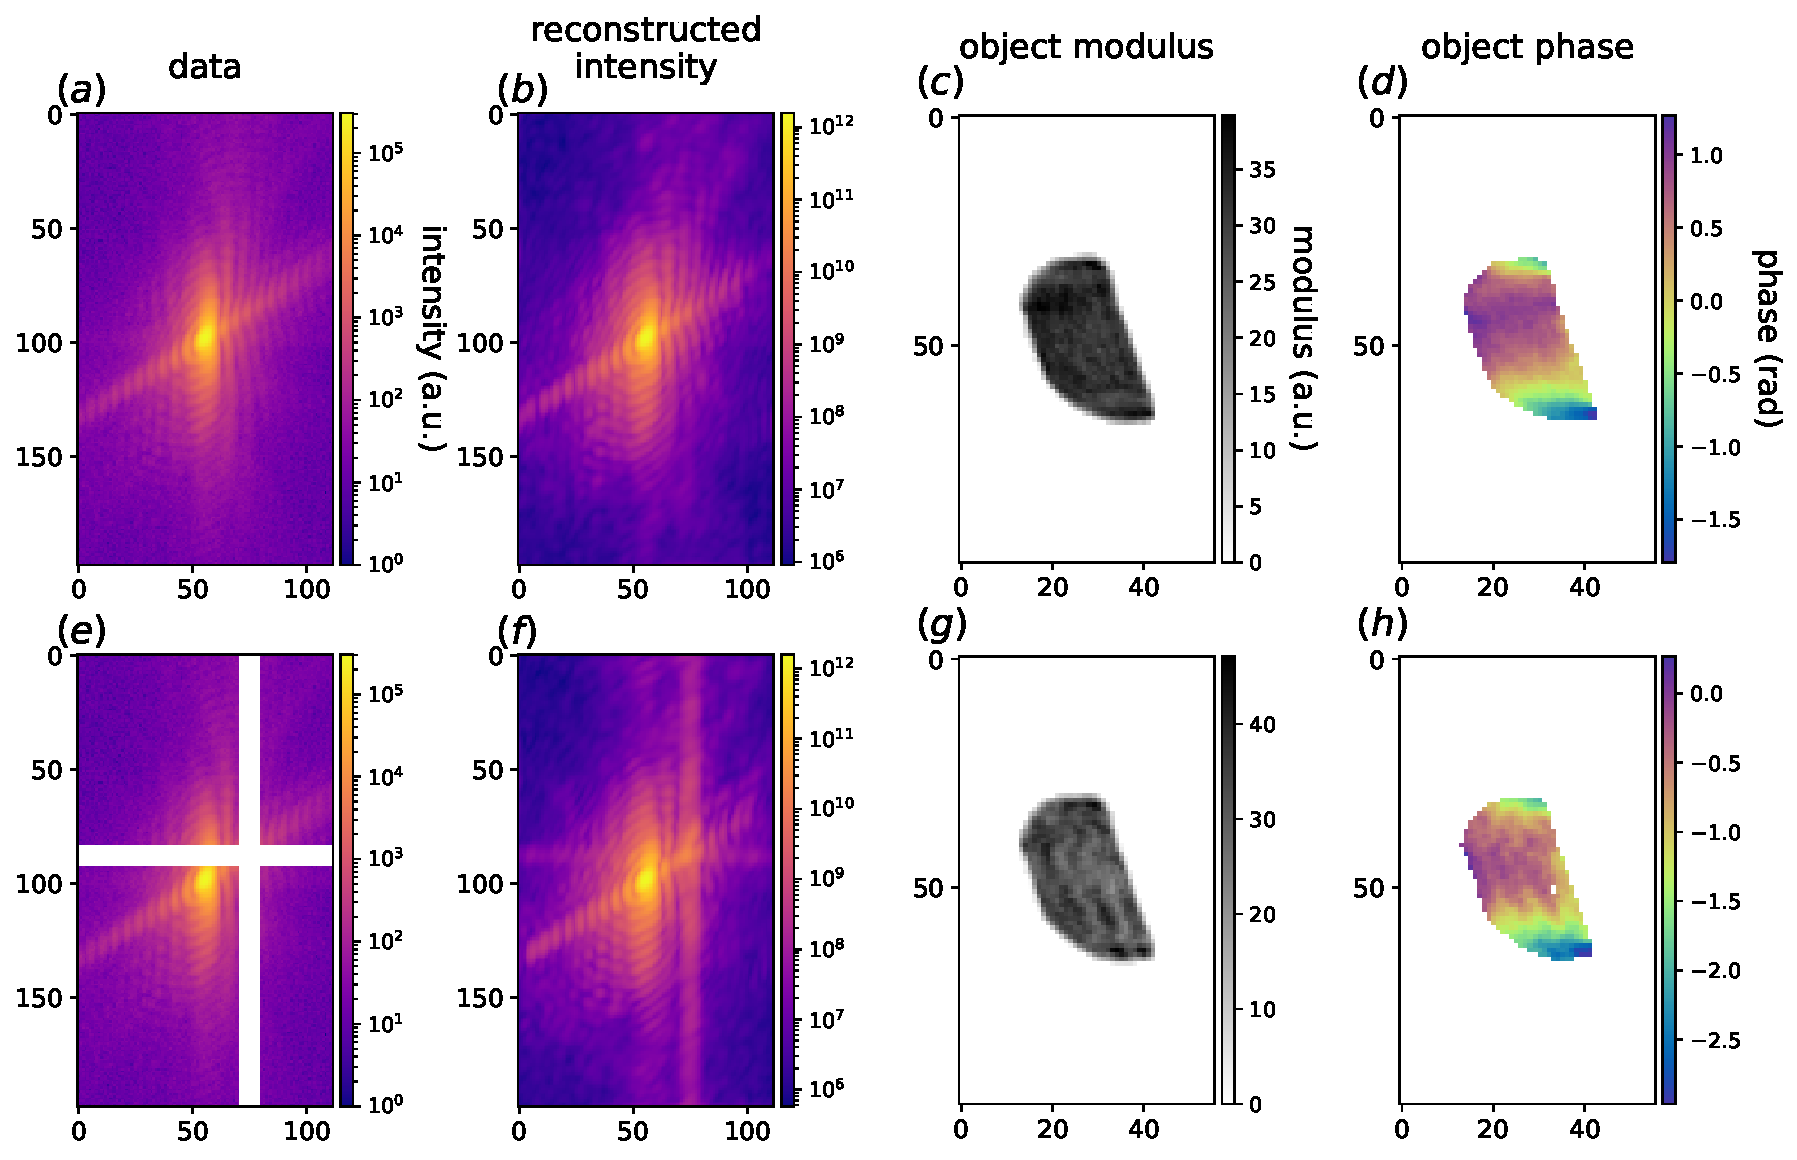
\includegraphics[width=\textwidth]{figures/Inpainting/gaps_mask.pdf}
    \caption{\textbf{Masking the gap region during phasing} 
    \textbf{(a)} The central xz slice of an experimental diffraction pattern. \textbf{(b)} The same slice of the diffracted
    intensity calculated from the retrieved object. Comparing this figure with \ref{fig:gap_intro}\textbf{(b)} one can see that
    when excluding the gap region from the phasing with a mask, the calculated intensity shows bright non-physical streaks 
    instead of the gaps. \textbf{(c - d)} xz slice of the modulus and phase respectively of the particle obtained from the 
    phasing of the gap affected data with a mask of the gap regions. Despite the much higher quality of the reconstruction, 
    one can notice some oscillatory artifacts appearing in both the modulus and the phase of the retrieved object. }
    \label{fig:gap_intro_mask}
    \end{figure}

Another, more invasive, option is to \textit{fill} these gaps with an estimate of the intensity distribution that
would be there, before the phase retrieval. These tasks of filling gap in images is usually referred to as ``inpainting''.
The following paragraph mentions the most relevant inpainting methods to give a context for our work.
    
\subsection{Background on Image Inpainting Research}

 
Computational image inpainting has been widely studied in the field of photography and imaging for many years \cite{Elharrouss_2019,reviewInpainting2021}. 
The inpainting problem can be defined as the task of utilizing known information extractable from the image, to repair
the parts where this information is missing, where for known information the colors, the textures and the semantic features
are intended. In the history of image inpainting a clear cut can be observed when deep learning methods have started to be employed.
For traditional inpainting, different techniques have been explored, from the texture synthesis methods pioneered by Efros and 
Leung \cite{Efros1999} to the use of PDEs as Navier-Stokes equations proposed by Bertalmio \textit{et al.} \cite{BertalmioNavierStokes}
and then again from sparse representations \cite{Mairal_sparse} to hybrid methods combining variational and statistical methods \cite{CedricAllene}

More recently instead, Deep Learning models, headed by Convolutional Neural Networks (CNN), have taken the place of more traditional 
methods as they can attain higher accuracy for more complex inpainting tasks. By undergoing a  
training process, CNNs can ``learn'' to recognize and reproduce the semantic features of the training dataset, and thus
leverage them during inference as additional information beside the colors and textures of the specific image to restore. 
As we have seen in \ref{ch:intro}, the typical CNN architecture for image generation consists of an encoder, which
retains the features of the input image and compresses them into a lower dimensional latent space, and a decoder, which
is responsible for the generation of the output image starting from the latent space. The model are then trained according 
to a loss function that pushes the model's predictions to be close to a given ground truth reference. 
In some cases, the loss function can be replaced by another CNN that is trained to discriminate true images from the ones
predicted by the model. These complementary networks are known as Generative Adversarial Networks (GAN), firstly 
proposed by Goodfellow \textit{et al.} \cite{goodfellow2014generativeadversarialnetworks}, and have also been used for 
image inpainting (e.g. \cite{gan_inpainting}). 
Since reviewing the vast amount of works about CNN for image inpainting is beyond the scope of this thesis and for more 
information, we redirect the reader to the reviews published by Elharrouss \textit{et al.} and Xu \textit{et al.} \cite{reviewInpainting2021,reviewInpaintingDL2023}.
as well as this blog article \cite{towardsdatascience_inpainting}. For what concerns the application of DL based 
inpainting for scientific imaging, early works date back to 2018 as in the case of Sogancioglu \textit{et al.} for x-ray 
human chest 2D radiographic images \cite{sogancioglu2018chestxrayinpaintingdeep} and to 2020 for 2D microscopic images \cite{microscopic_inpainting_2020}.
A couple of years later Tanny Chavez and coauthors published a paper comparing the performances of different CNN models 
for the inpainting of 2D x-ray diffraction images \cite{chavez_comparison_2022}. The work is precisely addressing the 
gap problem for x-ray detectors used for powder diffraction measurements and is awarding UNet and Mixed Scale Dense (MSD) 
models for the best performances on experimental data. The DL models outperform interpolations obtained with biharmonic functions
across 7 and 17 pixel-wide gaps. This work has been of inspiration for the design of our DL model for BCDI gaps inpainting.
In the same year, another work on DL based inpainting for x-ray detector gaps was published by Alfredo Bellisario 
and coauthors \cite{bellisario_noise_2022}. The authors tested a UNet-like model on the inpainting of 2D simulated, noiseless
coherent diffraction patterns against gaps of different sizes (2 to 20 pixels) along the central row. The gaps were 
placed such that the center of the peak was covered, a choice that, as we will see later, yields better results than 
predictions on peripheral areas. To our knowledge, at the time of writing, no other works about deep learning based inpainting
for X-ray detector gaps are present in the literature. \\

\section{Model design: 2D case}\label{sec:model}

On the heels of the last mentioned works we have started to tackle the detector gaps problem for BCDI using CNNs. For simplicity, we started off with 2D
case, using simulated diffraction patterns and inpainting randomly placed vertical gaps of different width. First, we created a training set of 
simulated data, composed of pairs of gap-affected images and corresponding gap-free ground truths, then built a U-Net-like model and trained it 
in a supervised fashion.

\subsection{Dataset creation}\label{sec:dataset_creation}

The creation of training datasets of simulated 2D BCDI patterns for both the gap-inpainting and phase retrieval tasks has followed the procedure
described in this paragraph.\\
In first place, once chosen the size of the array, a randomly shaped polygon is created in the center using \texttt{scipy.spatial.ConvexHull} 
function. This guarantees the object to have a compact support with homogeneous electron density as assumed for BCDI. Subsequently, 
a random phase field of the same size with variable phase range and correlation length is generated thus the complete complex object is formed.
In order to make the object more realistic a Gaussian filter and Gaussian random noise are applied to the object's modulus, so to smoothen the edges 
and simulate real cases respectively. At this point the object is resized to the shape required to match the chosen oversampling ratio and the 2D
Discrete Fourier Transform is computed. As last stage, Poisson noise is added to the diffraction patterns with different magnitudes to simulate 
various X-ray flux conditions. \\
Datasets contain a number of diffraction patterns in the order of thousands and for each of them the random variables are different as well as the 
oversampling ratios. In the datasets for the training of phase retrieval models, the reciprocal space phase corresponding to each diffraction pattern
is saved as well and used as ground truth label. 
For inpainting tasks a randomly located vertical gap mask was created and applied to the intensity data. In some cases cross-shaped gaps were 
added instead to simulate the experimental condition of the Bragg peak in the vicinity of the corner of the sensing area. 
The size of the gaps was chosen to be consistent across the dataset and four different cases were studied (3px, 6px, 9px, 12px).

\begin{figure}[h]
    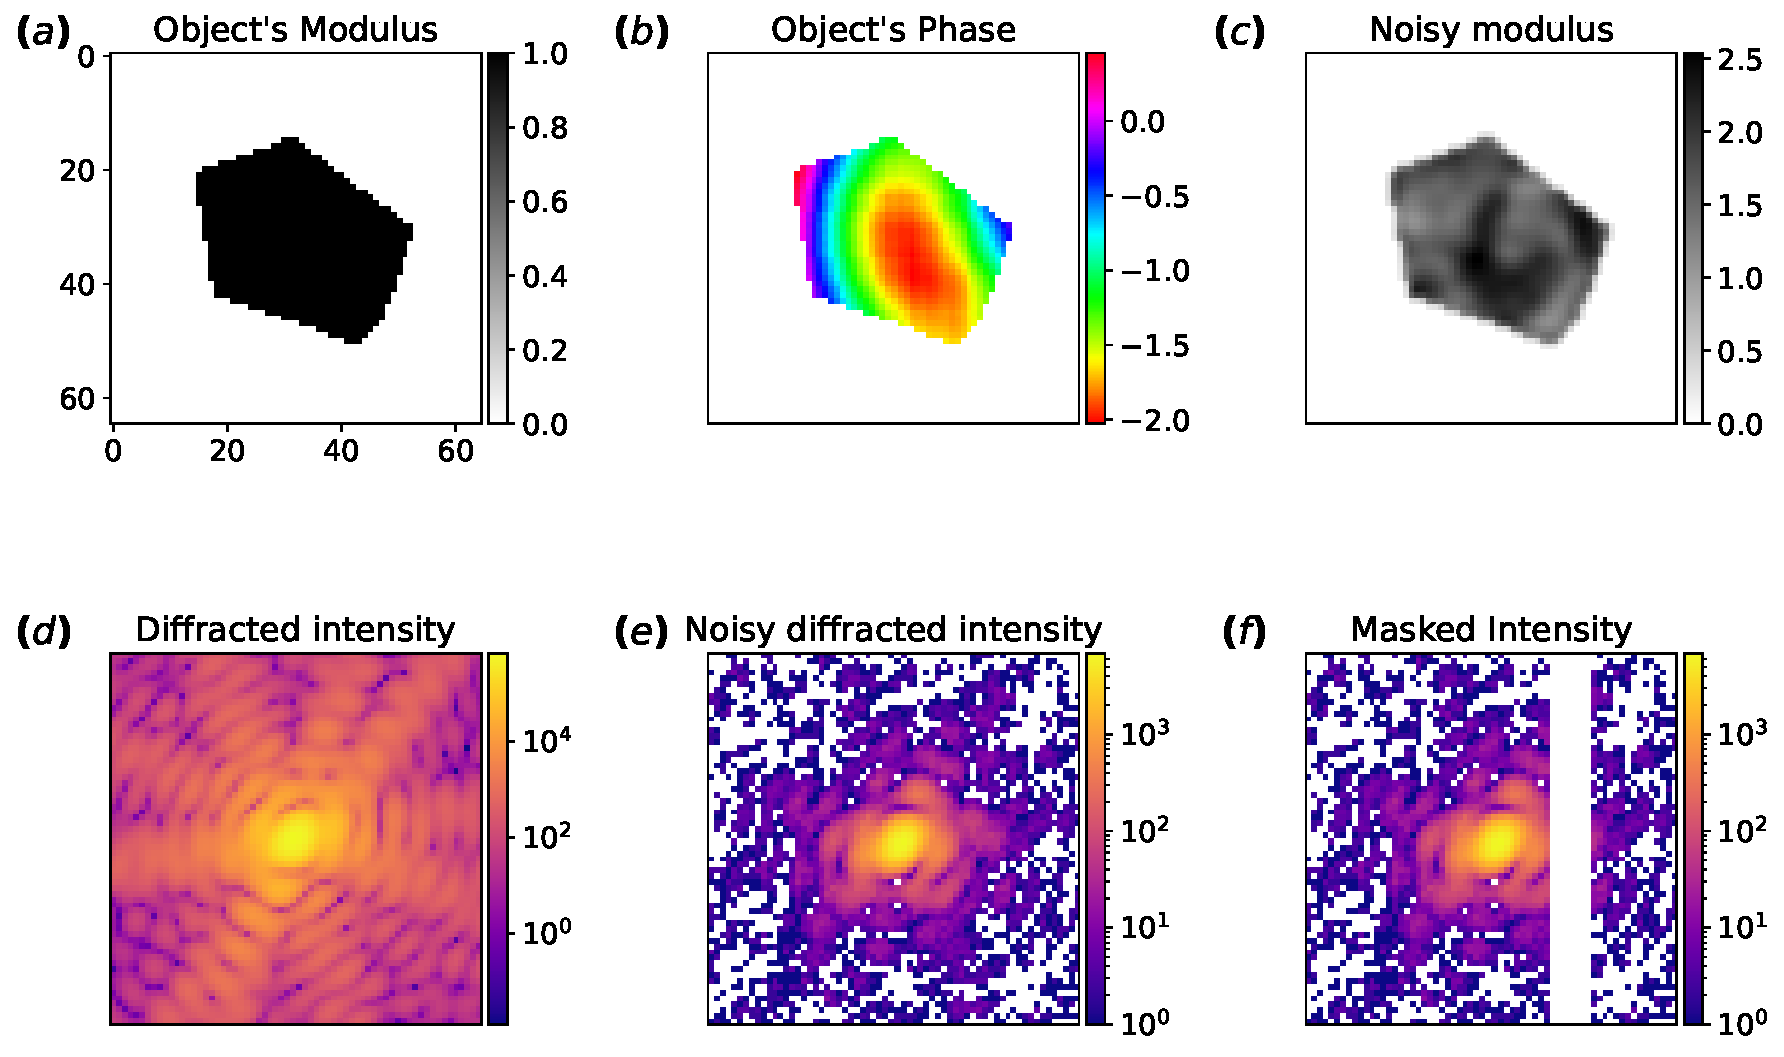
\includegraphics[width=\textwidth]{figures/Inpainting/2D_dataset_creation.pdf}
    \caption{\textbf{Steps for the simulation of a single 2D diffraction pattern} 
    \textbf{(a)} Simulated modulus of a 2D object with random shape and compact support. \textbf{(b)} Simulated object's phase
    \textbf{(c)} Object's modulus after smoothening the edges and adding random Gaussian noise. \textbf{(d)} Squared modulus of the Fourier Transform
    of the complex object (in log scale). The object is first padded with zeros to match the chosen oversampling ratio.
    \textbf{(e)} Poisson noise is added to the simulated diffracted intensity. \textbf{(f)} A 6 pixel-wide
    vertical gap is added to the diffracted intensity at a random position.}
    \label{fig:2D_dataset_creation}
\end{figure}


\subsection{2D Model design}

The 2D model that we have implemented is a U-Net that takes in input batches of 32 simulated BCDI patterns affected 
by both vertical and cross-shaped gaps. Each diffraction pattern is transformed into logarithmic scale to enhance the 
spatial features and then normalized between 0 and 1. This last passage is proven to be convenient to any DL model \cite{efficientBackProp}.
Regarding the logarithmic transformation, it is important to notice that in order to avoid problems for zero intensity
values, the $\log(I+1)$ was taken.
The shape of each image was chosen to be of $128\times128$ pixels. The inputs go through five convolutional blocks 
inside each of which a convolutional layer, a Leaky ReLU activation function and a MaxPooling operation are applied. 
The tensor's dimensionality is so reduced down to $2\times2$ while the channel dimension is brought up to 768 filters 
while the kernel size is kept at $3\times3$. In this first model we directly pass this $(32,2,2,768)$ tensor to the 
decoder that, mirroring the encoder, is composed of five blocks inside each of which there is a transposed convolutional layer
that upsamples the feature maps (stride = 2) and a Leaky ReLU activation function. We also implemented skip connections connecting each encoder block
to its corresponding shape-like decoder block. This measure has proven to be beneficial for the information flow between
encoder-decoder \cite{li_visualizing_2017}. The last activation layer of the model is a sigmoid function that guarantees an output bounded between 0 and 1 \\ 

In the first place we utilized a simple Mean Squared Error (MSE) as cost function inside the gap region only, training 
the model on 12'000 diffraction patterns over 10 epochs, with ADAM optimizer and a learning rate of $10^{-4}$. 
We have tested the Mean Absolute Error (MAE) and the Structural Similarity Index Measure (SSIM) \cite{ssim}
as well afterwards and compared the results after the same training.
Here in Fig. \ref{fig:loss_comparison} we report the comparisons for the 9 pixel-wide gap on a test simulated diffraction
pattern. The accuracy scores were calculated using the Pearson Correlation Coefficient (PCC).

\begin{equation}
    PCC = \frac{\sum_{i\in \text{gap}}(\textbf{I}_i^{\text{true}} - 
    \langle \textbf{I}^{\text{true}}\rangle)(\textbf{I}_i^{\text{pred}}-
    \langle\textbf{I}^{\text{pred}}\rangle)}{\sqrt{\sum_{i\in \text{gap}}^{}(\textbf{I}_i^{\text{true}} - 
    \langle \textbf{I}^{\text{true}}\rangle)^2}\sqrt{\sum_{i\in \text{gap}}^{}(\textbf{I}_i^{\text{pred}}-
    \langle\textbf{I}^{\text{pred}}\rangle)^2}},
        \label{eq:accuracy}
\end{equation}

Where \textbf{I} is the intensity inside the gap.

\begin{figure}[h]
    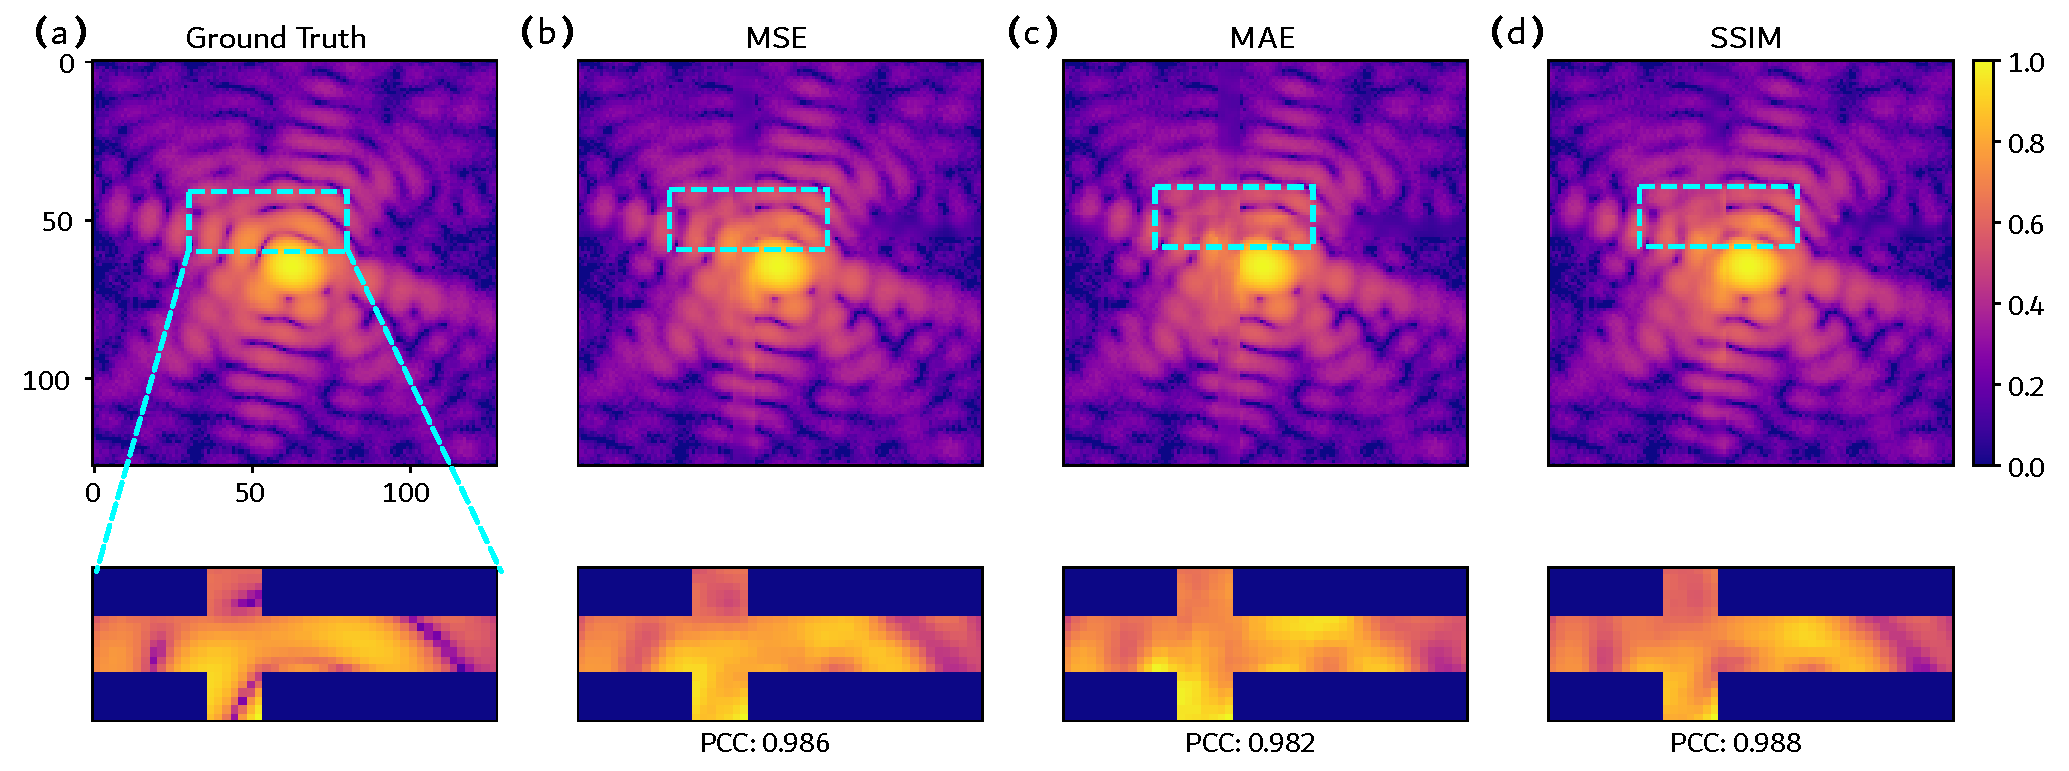
\includegraphics[width=\textwidth]{figures/Inpainting/loss_comparison.pdf}
    \caption{\textbf{Comparison of different losses} Results on a test simulated diffraction pattern for the inpainting 
    of a 9 pixel-wide cross-shaped gap produced by the same UNet model trained for 10 epochs with different loss functions. 
    \textbf{(a)} Shows the ground truth. \textbf{(b)} The prediction of the model trained with the MSE, \textbf{(c)} 
    with the MAE, \textbf{(d)} with the SSIM. Corresponding accuracy scores calculated with the Pearson Correlation 
    Coefficient (PCC) are shown as well. While MAE fails to recover the oscillations, SSIM yields better results.}
    \label{fig:loss_comparison}
\end{figure}

In the light of these results, we have decided to discard the MAE metric and adopt instead the sum of MSE and SSIM. 
At last, another term computing the MSE between the \textit{gradients} of the ground truth and predicted intensity inside
the gap region was added in the definitive loss function.\\

Once established what we considered the best loss function, we have explored different models. 
Following the work of Chavez \textit{et al.} mentioned above (\cite{chavez_comparison_2022}), we considered a 
Mixed-Scale Dense Network (MSD-Net). The advantage of this type of networks is the significant reduction of trainable
parameters, and the use of \textit{dilated} convolutions with respect to U-Net ones. While the former property guarantees
faster trainings and lower chances of overfitting, the latter enhances the capture of long-range correlations. Moreover, 
in a MSD-Net, the image's spatial dimensions are kept constant throughout the whole network as no downsampling nor upsampling is operated.
The MSD-Net that we have used consists of sequential blocks in each of which the input is transformed by two different 
convolutional layers with growing dilation rates. Each output of the convolutional layers is concatenated to the input 
feature map and the result is passed to the following block. While the kernel size is kept constant to $3\times3\times3$ pixels
the dilation rate increases linearly from 1 to 30. The last layer is a sigmoid function as well as for the U-Net. 
The total number of trainable parameters is in the order of 320'000, two orders of magnitude lower than the U-Net.
\\
In order to combine the hierarchical dimensionality reduction of the U-Net with the fine-features capturing of the MSD-Net 
we have implemented a modified U-Net that adopts dilated convolutions inside the first three encoder blocks. In particular, 
they return the input tensor concatenated with the outputs of four dilated convolutional layers computed
from the input. Dilation rates of (16,8,4,2), (10,5,3,1) and (5,3,2,1) were chosen respectively. As the MaxPooling 
operation down-samples the feature maps into smaller sizes, we limited the dilated convolutions to the first three 
blocks. Moreover, we utilized them in the encoder layers only as they are mostly used for feature extraction \cite{dilated_conv}.
The characteristics of each model are summarized in form of pseudo - code in Table \ref{tab:model_comparison}.
\\

The three different models have been trained with a combined loss function (MSE + SSIM + MSE on the gradients ) on the 
same training dataset for 10 epochs each.  The results showed poor performances of the MSD-Net with respect to the two 
U-Nets. Slightly higher accuracy was achieved by our modified U-Net. 

\begin{figure}[h]
    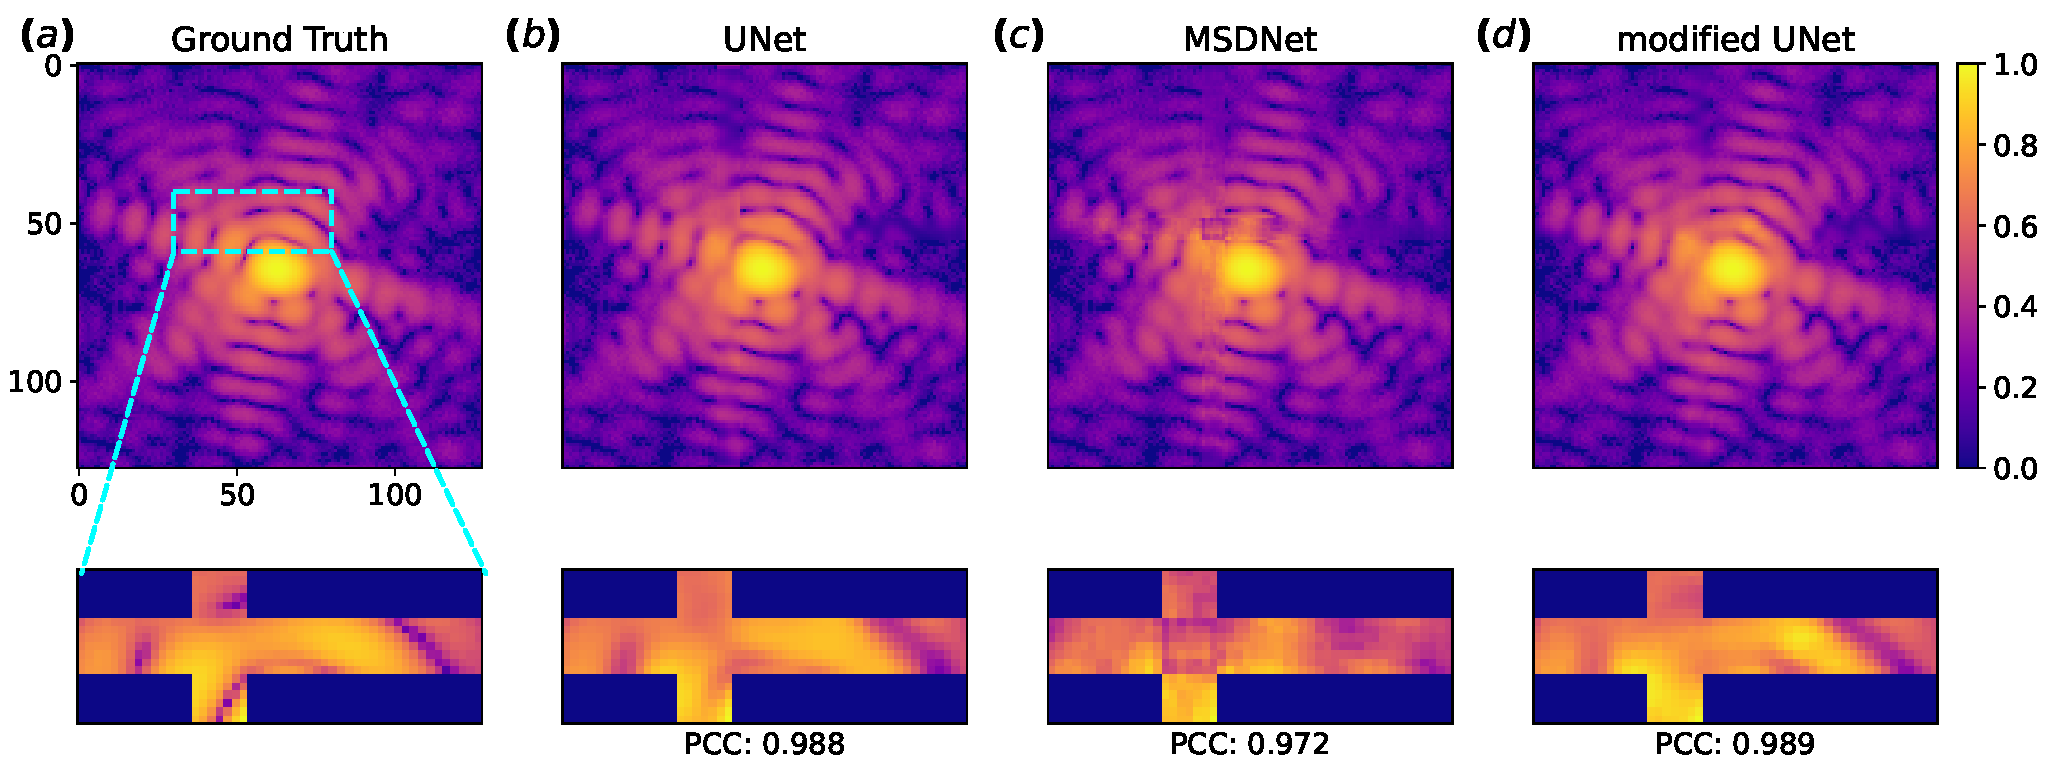
\includegraphics[width=\textwidth]{figures/Inpainting/model_comparison.pdf}
    \caption{\textbf{Comparison of different models} Results on a test simulated diffraction pattern for the inpainting 
    of a 9 pixel-wide cross-shaped gap using three different models trained with the same loss function.
    \textbf{(a)} Shows the ground truth. \textbf{(b)} The prediction of the U-Net, \textbf{(c)} 
     of the MSD-Net, \textbf{(d)} of the modified U-Net. Corresponding accuracy scores calculated with the Pearson Correlation 
    Coefficient (PCC) are shown as well.}
    \label{fig:models_comparison}
\end{figure}


\begin{table}[h!]
    % \small 
    %  or 
    \scriptsize
    \centering
    % \resizebox{\textwidth}{!}{%
    \begin{tabular}{|>{\centering\arraybackslash\bfseries}p{1.2cm}|p{4.5cm}|p{4.5cm}|p{4.5cm}|}
    \hline
     & \textbf{U-Net} & \textbf{MSD-Net} & \textbf{Unet\_mod} \\ \hline
    block1 & 
    \begin{lstlisting}[basicstyle=\tiny\ttfamily, xleftmargin=-1em]
    def encoder_block(x_input, num_filters, ker):
        s = Conv2D(num_filters, ker,'leaky_relu')(x_input)
        x = MaxPool2D(2)(s)
        return x, s
    \end{lstlisting} 
    & \begin{lstlisting}[basicstyle=\tiny\ttfamily, xleftmargin=-1em]
    def MSD_block(x, in_channels, dilations,kernel_size=3):  
        if isinstance(dilations, int):  
            dilations = [(j % 10) + 1 for j in range(dilations)]  
        out_channels = in_channels + len(dilations)  
        for d in dilations:  
            x1 = Conv2D(out_channels//2,kernel_size,1, dilation_rate=dilation, 'same', 'leaky_relu')(x)
            x = tf.concat([x1,x] ,axis = -1)
        return x, out_channels
    \end{lstlisting} 
    &
    \begin{lstlisting}[basicstyle=\tiny\ttfamily, xleftmargin=-1em]
    def encoder_block_mod(x_input, ker, num_filters, rate):
        f = num_filters // 4
        s = tf.concat([x_input] + [Conv2D(f, ker, dilation_rate=r, 'leaky_relu')(x_input) for r in rate], axis=-1)
        return MaxPool2D(2)(s), s
    \end{lstlisting} \\ \hline
    block2 
    &
    \begin{lstlisting}[basicstyle=\tiny\ttfamily, xleftmargin=-1em]
    def decoder_block(x_input, num_filters, ker, skip_input = None):
    
        if skip_input is not None:
            x_input = Concatenate()([x_input, skip_input])
            
        x = Conv2DTranspose(num_filters, ker, strides=2, 'leaky_relu')(x_input)
        return x
    \end{lstlisting} 
    & 
    &
    \begin{lstlisting}[basicstyle=\tiny\ttfamily, xleftmargin=-1em]
    def decoder_block(x_input, num_filters, ker, skip_input = None):
    
        if skip_input is not None:
            x_input = Concatenate()([x_input, skip_input])
            
        x = Conv2DTranspose(num_filters, ker, strides=2, 'leaky_relu')(x_input)
        return x
    \end{lstlisting} \\ \hline
    
    body & 
    \begin{lstlisting}[basicstyle=\tiny\ttfamily, xleftmargin=-1em]
        x, s1 = encoder_block(inputs, 48,3)        
        x, s2 = encoder_block(x, 96,3)             
        x, s3 = encoder_block(x, 192,3)           
        x, s4 = encoder_block(x, 384,3)           
        x, s5 = encoder_block(x, 768,3)          
    
        x = Conv2D(1536,3, 'leaky_relu')(x) 
    
        x = decoder_block(x,768,3)
        x = decoder_block(x,384,3, s5)
        x = decoder_block(x, 192,3,s4)
        x = decoder_block(x, 96,3,s3)
        x = decoder_block(x, 48,3,s2)
        
        x = Conv2D(24,5,'leaky_relu')(x) 
        x = Conv2D(12,5,'leaky_relu')(x)
        x = Conv2D(6,5,'leaky_relu')(x)
        
        out = Conv2D(1,5,'sigmoid')(x)
    \end{lstlisting} 
    & 
    \begin{lstlisting}[basicstyle=\tiny\ttfamily, xleftmargin=-1em]
        x,out_ch = MSD_block(inputs,1,[1,2])
        x,out_ch = MSD_block(x,out_ch,[3,4])
        ...
        ...
        x,out_ch = MSD_block(x,out_ch,[31,32])
        out = Conv2D(1,3,'sigmoid')(x)
    \end{lstlisting} 
    &
    \begin{lstlisting}[basicstyle=\tiny\ttfamily, xleftmargin=-1em]
        x, s1 = encoder_block_mod(inputs,3,48,[16,8,4,2])   
        x, s2 = encoder_block_mod(x,3, 96,[10,5,3,1])       
        x, s3 = encoder_block_mod(x,3, 192,[5,3,2,1])           
        x, s4 = encoder_block(x, 384 ,3)            
        x, s5 = encoder_block(x, 768, 3)                    
        
        x = Conv2D(1536,3,'leaky_relu')(x)
        
        x = decoder_block(x,768,3)    
        x = decoder_block(x,384,3,s5)  
        x = decoder_block(x,192,3,s4)  
        x = decoder_block(x,96,3,s3) 
        x = decoder_block(x,48,4,s2)  
    
        x = Concatenate()([x, s1])
        x = Conv2D(24,5,'leaky_relu')(x) 
        x = Conv2D(12,5,'leaky_relu')(x)   
        x = Conv2D(6,5,'leaky_relu')(x)
    
        out = Conv2D(1,3,'sigmoid')(x)
    \end{lstlisting} \\ \hline
    parameters & 31,827,673 & 322,458 & 32,652,337 \\ \hline
    \end{tabular}
    \caption{Comparison of Unet, MSDNet, and Unet\_mod components.}
    \label{tab:model_comparison}
\end{table}

We conclude here the introductory studies on 2D simulated data. These preliminary tests served to get familiar with 
the different DL architectures and loss functions and select the optimal choices for the inpainting of BCDI detector
gaps. 

\subsection{Accuracy VS Gap position}

Before moving to the 3D case, it is worth spending a few words on the assessment of the DL model upon different conditions.
We leave the assessment of the prediction accuracies against the gap size for the 3D case and will focus instead on two
other evaluations. Namely, the accuracy as function of the position of the gap inside the diffraction pattern and the 
as a function of the oversampling ratio.
For the first test we have simulated 150 2D diffraction patterns from random particles shapes, random oversampling ratios
and Poisson noise intensity. For each diffraction pattern we have then placed a vertical 9 pixel-wide gap at all positions
from left to right, computed the DL prediction and corresponding accuracy score when compared to the ground truth. The 
accuracy was again calculated with the Pearson Correlation Coefficient. We have then averaged this score for each 
gap position, over the 150 diffraction patterns and plotted the result as a function of the gap position. Fig. \ref{fig:accVSpos} 
shows the resulting curve that clearly highlights that the model performs better regions with high intensity. 
This can be qualitatively explained with different reasons: (i) central regions have larger features both because of the 
nature of the Bragg peak, and because of the lower noise level. This makes it easier for the model as it reduces the 
complexity of the prediction. (ii) As we move away from the center of the Bragg peak, the Signal to Noise Ratio (SNR) 
decreases, along with the \textit{density of signal}. High accuracy scores in these regions would require the model to be 
able to predict noise correctly which is by definition impossible as it is an uncorrelated random process. One could argue 
that the accuracy curve would follow the statistical distribution of the gap positions inside the DL model training dataset.
However, each mask has been applied at a position drawn from a discrete uniform probability function spanning in the full
data size, thus we exclude this hypothesis. 

\begin{figure}[h]
    \centering
    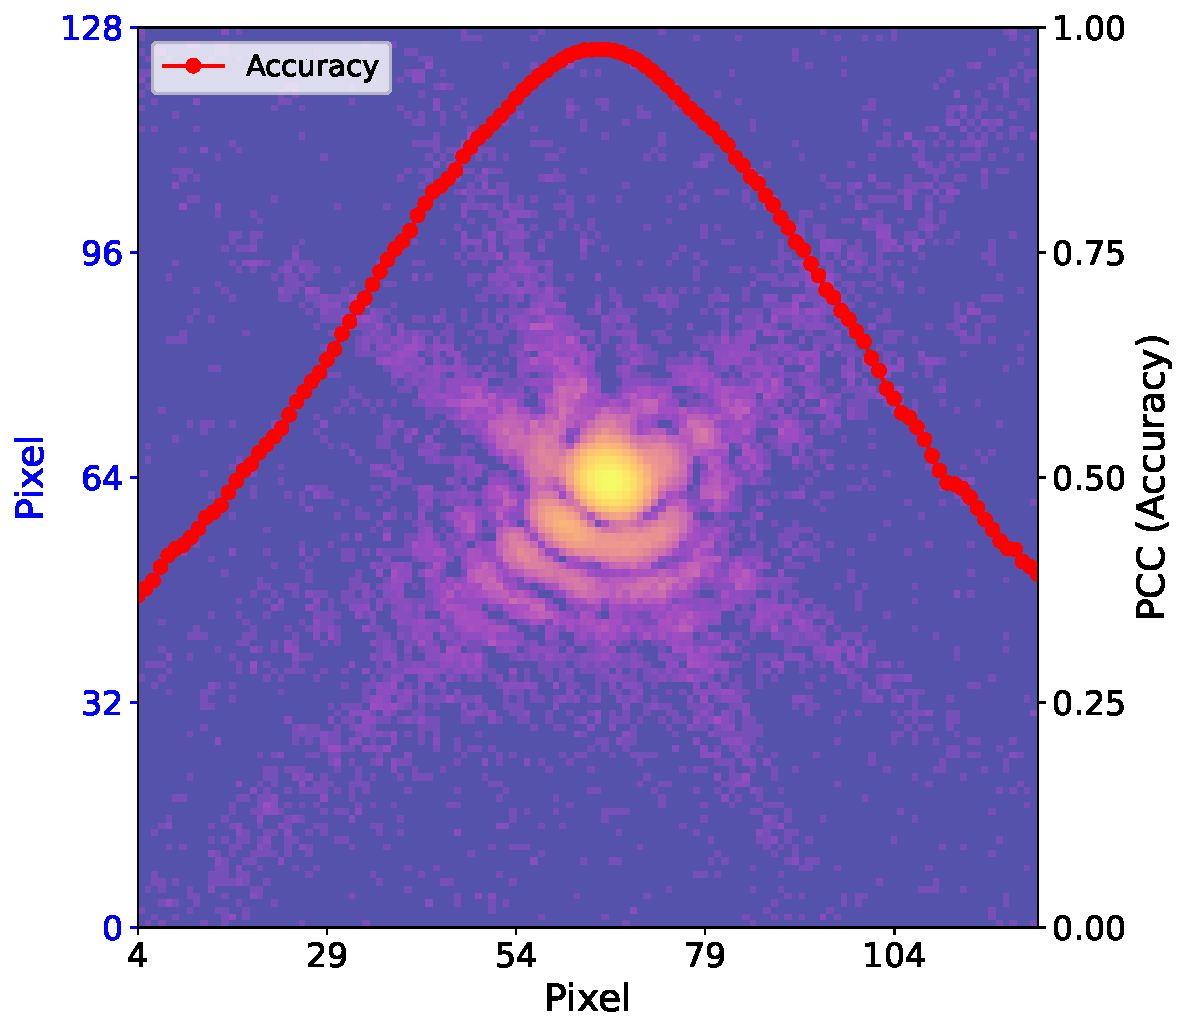
\includegraphics[width=.7\textwidth]{figures/Inpainting/2D_acc_pos.pdf}
    \caption{\textbf{(Accuracy VS Gap position)} Average Pearson Correlation Coefficient calculated over 150 
    9 pixel-wide vertical predicted gaps for each position of the gap inside the diffraction patterns. The model 
    shows higher accuracies for high intensity regions.}
    \label{fig:accVSpos}
\end{figure}

To conduct the second test, we simulated 150 diffraction patterns for the same particle varying gradually the oversampling
ratio between 2 and 6. For each image we have then applied a 9 pixel-wide vertical gap at all $X$ positions and performed 
the DL prediction. The accuracy scores have been averaged for each prediction in the same image and plotted against the oversampling 
(Fig. \ref{fig:accVSovs}). As expected from the above considerations, the model performs better for larger oversampling ratios, 
because of the bigger size of the features with respect to the gap width and because of the more uniform \textit{density of signal}.
About this last concept, it is worth clarifying that, for a given particle, the total amount of intensity in the
diffraction patterns is in principle constant regardless of the oversampling ratio as it is fixed by Parseval theorem.
However, if the size of the dataset is kept fixed for different oversamplings, the effect is the same of a zoom lens
that increases or reduces the field of view. Therefore, while for low oversampling ratios the full peak is recorded, 
for higher ones the peak is cropped, and less intensity is present in the image. This effect, coupled with the typical radial
intensity decay of Bragg peaks and the presence of Poisson noise, makes largely oversampled BCDI patterns having a smaller
and more uniform \textit{density of signal}, intended as the amount of information per pixel. On the contrary, for low 
oversampling ratio the \textit{density of signal} is less uniform as it is high inside bright regions (lot of information
concentrated in few pixels) and low in noisy regions far from the peak. It follows that in order to properly assess the accuracy
against the oversampling ratio one should consider diffraction patterns over the same extent in Q-space, thus changing 
the size of the images. This more accurate evaluation was carried out for the 3D case and can be found in the next section.

\begin{figure}[h]
    \centering
    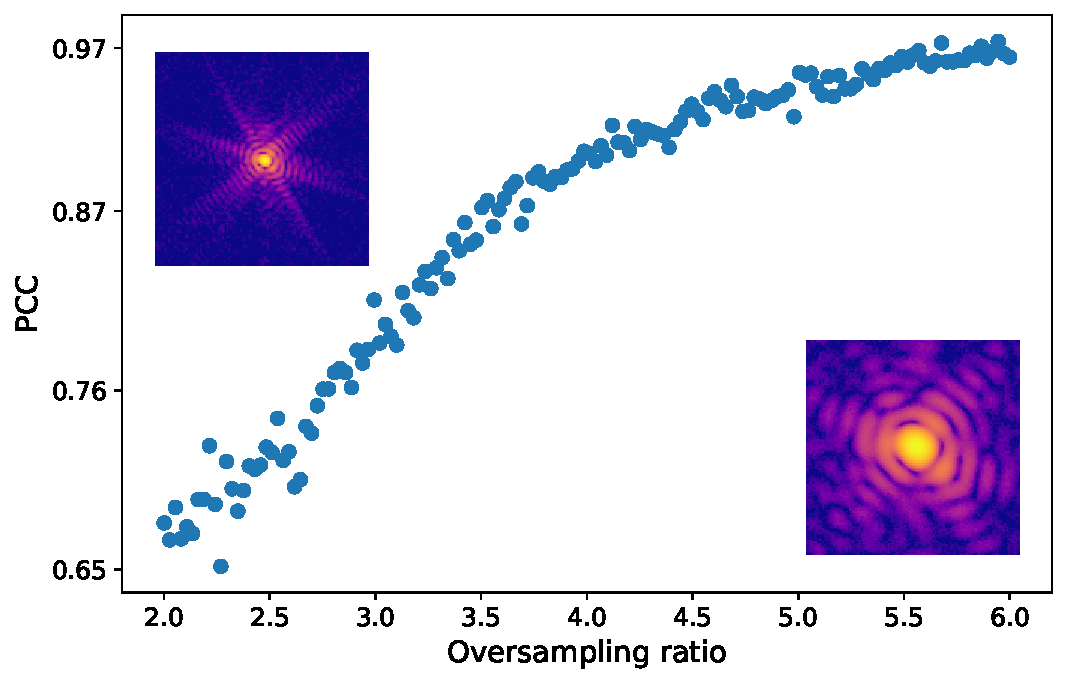
\includegraphics[width=.7\textwidth]{figures/Inpainting/2D_acc_ovs.pdf}
    \caption{\textbf{(Accuracy VS Oversampling ratio)} Average Pearson Correlation Coefficient calculated over 280
    9 pixel-wide vertical predicted gaps for each position of the gap inside the diffraction patterns. The model 
    shows higher accuracies for high intensity regions.}
    \label{fig:accVSovs}
\end{figure}

\section{3D case - Patching approach}\label{sec:patching}

When considering the 3D case, and especially the experimental conditions, there are a few practical issues that needs
to be overcome. In fact, experimental BCDI datasets that are more often affected by detector's gaps are necessarily large
datasets (e.g. $512 \times 512 \times N_{\text{rocking\_steps}}$). Training a U-Net like model for 3D images of that size is 
overly expensive in terms of computing memory and time. Moreover, a common problem with this type of architectures is that
the size of the images they can process is fixed by the first initialization. This means that one would need to resize, via 
binning or interpolation, the experimental datasets to the shape accepted by the DL model, and back to the original
shape after the inpainting. Besides the impracticality, these operations are not recommended as they induce further
modification and information loss to the original data. For these reasons we have opted for a patching approach that 
loosens these constraints while preserving sufficiently high accuracies. \\

The patching method exploits the regularity of the oscillations within BCDI datasets. The periodicity of the fringes 
in reciprocal space, peculiar property of this coherent diffraction technique, can be observed by eye and in many cases 
makes the prediction inside a gap region intuitively possible starting from just a few neighboring pixels. 
In our case we have decided to work with 32 pixel-sided cubic sub-volumes (patches from now on) cropped out of entire diffraction 
patterns. Among the ``GPU-friendly'' tensor sizes \cite{nvidia_tensor_cores_optimization} we opted for 32 as good trade-off
between amount of contained information and computing power required for training and inference. 

\subsection{Dataset creation}
The training dataset consists of 50\% patches from experimental data and 50\% from simulated data.
The experimental measurements were acquired at the ID01 beamline of the ESRF during different beamtimes on different particles.
Namely, (i) Pt particles dewetted on sapphire and YSZ (yttria–stabilized zirconia) with Winterbottom shape, 
measured under various temperatures and gas conditions, (ii) Pd and PdCe particles on glassy carbon, with
Wulff shape, measured in an electrochemical environment following hydrogen loading. (iii) Ni particles on sapphire undergoing
changes during $CO_2$ adsorption and (iv) cubic $CaCO_3$ particles on glassy carbon.
\\
The synthetic diffraction patterns were instead simulated in three steps. The first step consisted in the creation of 
simulated 3D particles of different shapes (Winterbottom, Wulff, Cubic, Octahedral and random) using pre-existing scripts
developed by Dr. Dupraz and Dr. Bellec \cite{lim_convolutional_2021}. These codes allow the user to construct a cubic FCC
crystal of a given element, taking into account the inter-atomic potential, the atomic mass
and the lattice parameter. The final particle is finally obtained by "cutting" off atomic planes along given (or random)
directions, depending on the chosen shape. We have simulated only Gold nano-particles and this is, in first approximation,
equivalent to any generic element as a different lattice parameter would just shift the Bragg peak to a different 
position in reciprocal space, with no significant alterations of the diffraction pattern.  
Each particle's configuration is then automatically saved in a LAMMPS-readable file. In a second stage, we perform 
energy relaxation using LAMMPS software for Molecular Dynamics. This step induces small displacements to the perfect 
lattice, especially near the surface. In the last stage, the 3D diffraction pattern of a selected Bragg 
reflection is computed using PyNX scattering package \cite{pynx_scattering}. This software, optimized for GPU 
acceleration, produces a 3D representation of a selected Bragg peak. 
It is then possible to adjust the parameters that control the oversampling ratio, the size of the array in which the 
Bragg peak is centered and the rotation of the Q-space. In our case we simulated 128 pixel-size cubic diffraction 
patterns and, in order to augment the training dataset, we did it for various oversampling ratios (from 2 to 5) and 
different rotations for each particle. As we have seen in Chapter (ref to introduction), in the kinematic scattering 
approximation the energy of the incident X-ray does not alter the diffraction pattern if not as a "zooming" factor. 
Thus, in our case we don't need to explicitly account for different energies as we already vary the oversampling ratio. 
Before taking portions of these simulated BCDI patterns, we added Poisson noise randomly scaling the $\lambda$ parameter
for each image.


\begin{figure}[h]
    \centering
    \begin{subfigure}{0.45\textwidth} % Adjust width as needed
        \centering
        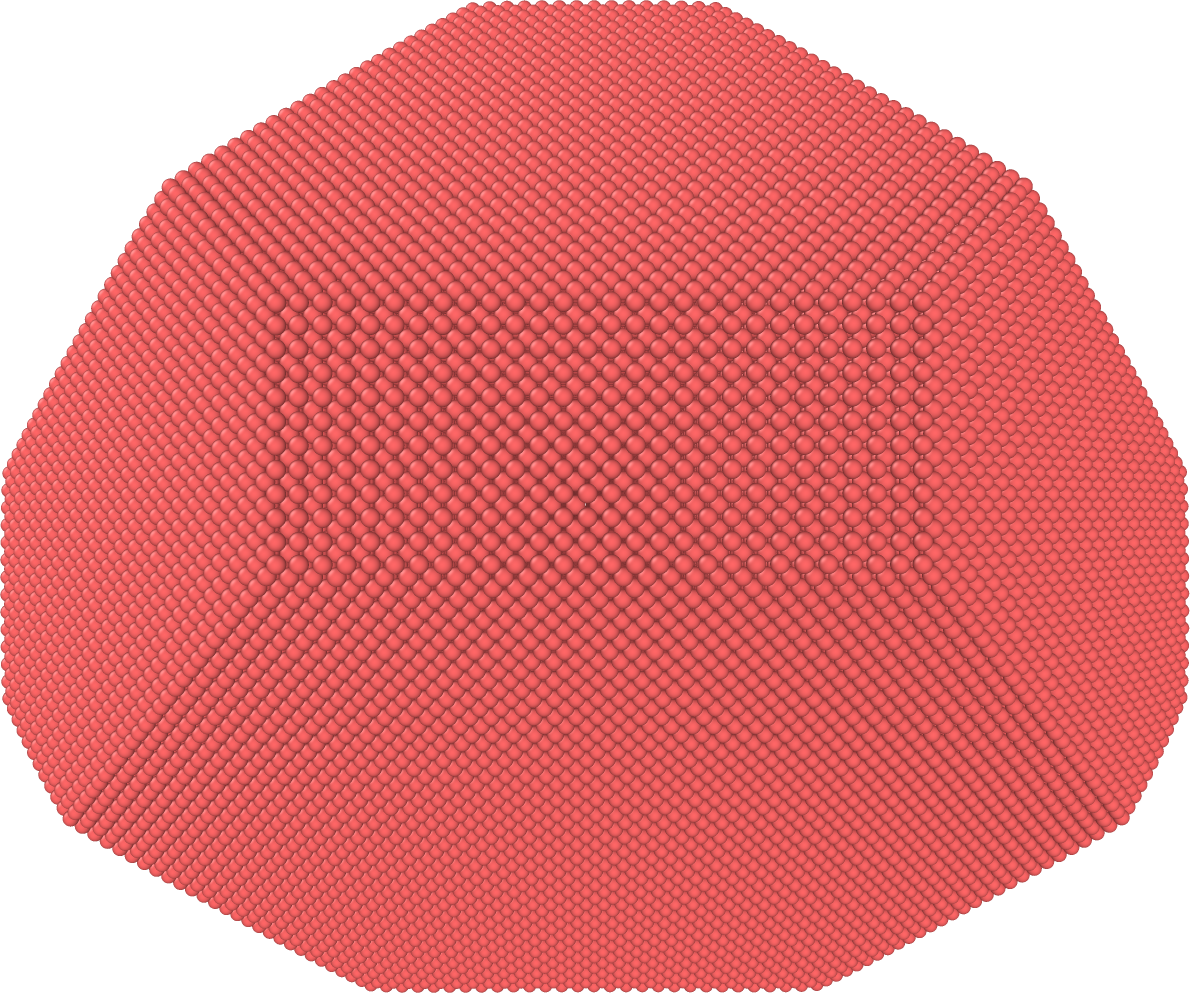
\includegraphics[width=\linewidth]{figures/Inpainting/crystal.png}
        \caption{\textbf{(a)}}
    \end{subfigure}
    \hfill
    \begin{subfigure}{0.45\textwidth}
        \centering
        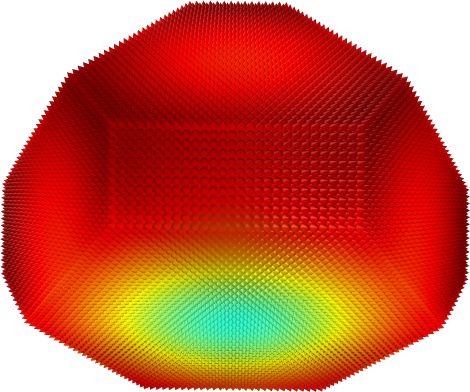
\includegraphics[width=\linewidth]{figures/Inpainting/displacement_field.png}
        \caption{\textbf{(b)}}
    \end{subfigure}
    \caption{\textbf{(a)} Simulated Au particle with Winterbottom shape (134114 atoms).\textbf{(b)} Atomic 
    displacement field of the same particle after LAMMPS energy relaxation. 
    It is evident the typical distribution at the interface with the substrate.}
    \label{fig:comparison}
\end{figure}


At this point, we proceeded with the extraction of sub-volumes taken at \textit{pseudo}-random locations inside each 3D pattern. 
The selection in fact was not totally random as we favored the extraction of sub-volumes from the outer regions, far from the 
center of the peak. There are mainly two reasons for this choice, namely (i) compensate the inherent uneven accuracy score against
the position of the gap (see Fig.\ref{fig:accVSpos}) by increasing the training data far from the center and (ii) emulate
as much as possible the experimental conditions, in which unavoidable gaps are typically far from the center of the peak.
For each sub-volume a 3D mask of the gap was created for different gap sizes (3,6,9,12 pixel-wide). The gap was placed 
vertically, in the center, along the third dimension, resulting in a ``empty slab''. Cross-shaped gaps were also 
included in the training dataset, with a population ratio of 1:5 compared to vertical gaps. They were created by 
adding a horizontal gap at a random height to an existing vertical gap.
The final training dataset consisted of 30'000 $32\times32\times32$ sub-volumes created as described above. 

\begin{figure}[h]
    \centering
    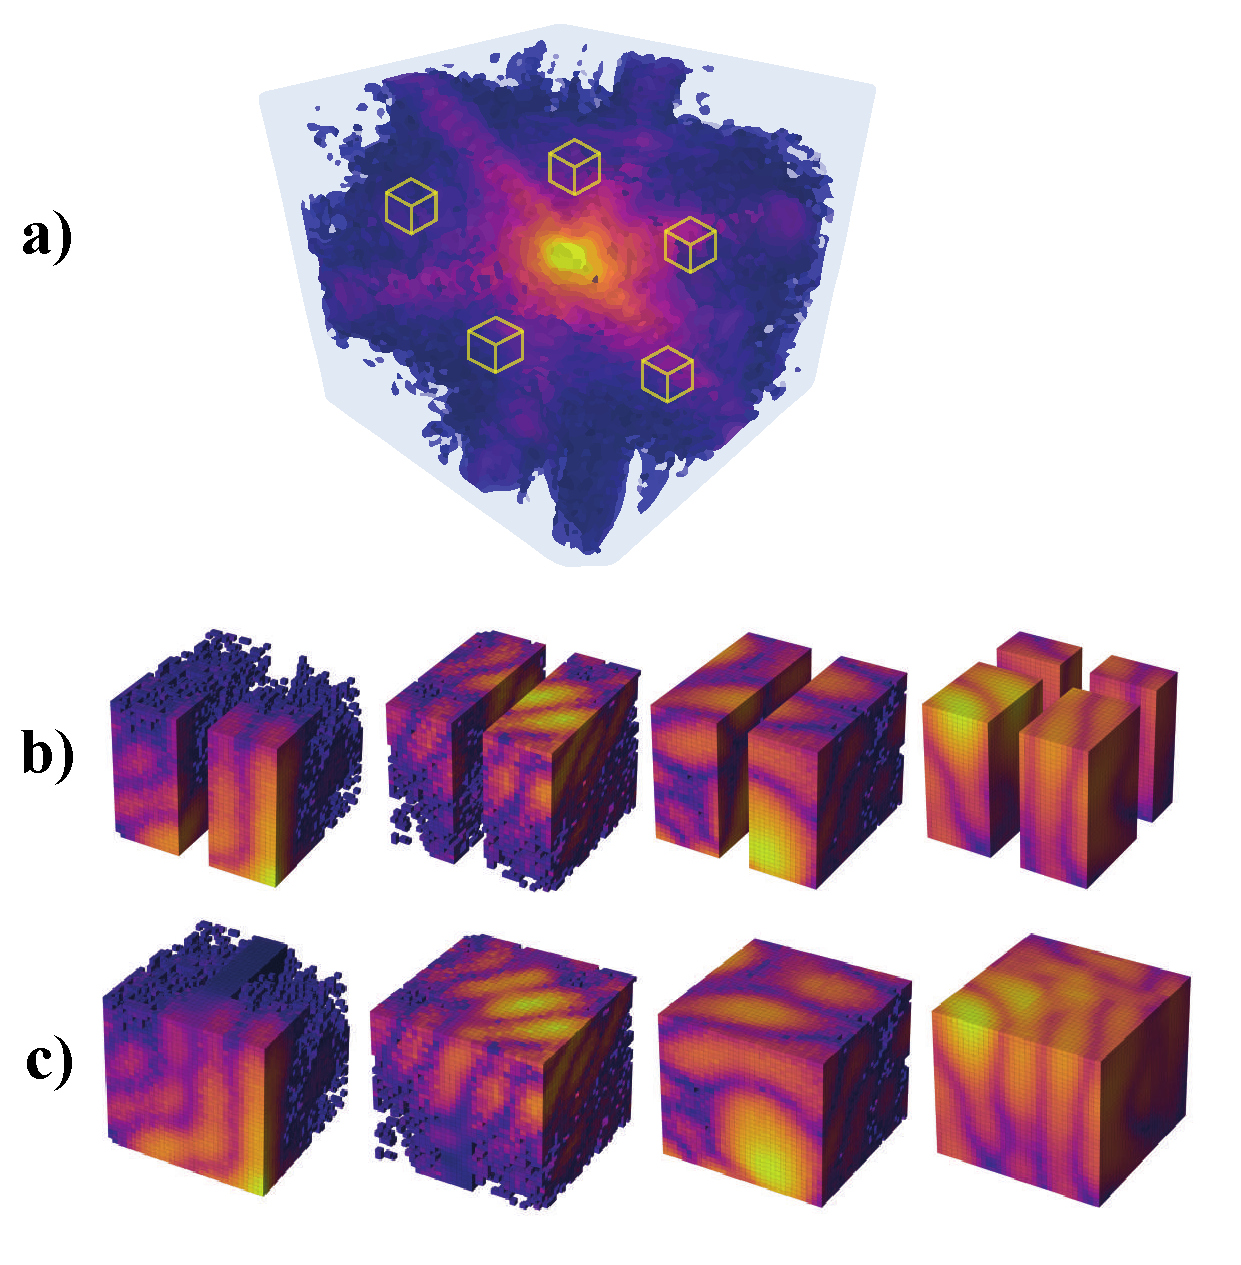
\includegraphics[width=.6\textwidth]{figures/Inpainting/process.pdf}
    \caption{\textbf{Schematic of the sub-volumes extraction.} \textbf{a)} The 3D BCDI diffraction pattern and the 
    sub-volumes. \textbf{b)} $32\times32\times32$ pixel-size sub-volumes with 9 pixel-wide vertical and cross-shaped gaps.
    \textbf{c)} Same sub-volumes with the DL inpainted gaps.}
    \label{fig:architecture3d}
\end{figure}

\section{3D model architecture}

The DL architecture used for the 3D patching inpainting is illustrated in Fig. \ref{fig:architecture3d}.  
Given the reduced size of the inputs, the encoder this time is composed of four blocks only, in each of which there
are convolutional layers and max pooling layers. The feature map is thus reduced to a $2\times2\times2\times478$ tensor 
before being passed to the decoder. Notice that, as introduced above in section Sec.\ref{sec:model}, we have employed
dilated convolutions in the first two blocks to enhance the extraction long-range correlated features. After four decoder
blocks we have put three simple convolutional layers with 24,12 and 6 channels respectively, in order to restore the possible
smoothing effect of the decoder. Same as in the 2D model, the last activation function is a sigmoid that ensures the output
to be in the range (0,1). 
The model contains 2'770'000 trainable parameters, significantly less than the 2D models working on full size patterns. 
\\
The training was performed loading batches of 32 images at the time over 100 epochs using ADAM optimizer \cite{ADAM}. 
We initialized the optimizer with a learning rate of $10^{-3}$ and decreased it progressively with the 
\texttt{ReduceLROn-Plateau} callback feature available in Tensorflow. In order to exploit at maximum the training 
dataset we left only 4\% and 2.5\% of the whole dataset for validation and testing respectively.  

\begin{figure}[h]
    \centering
    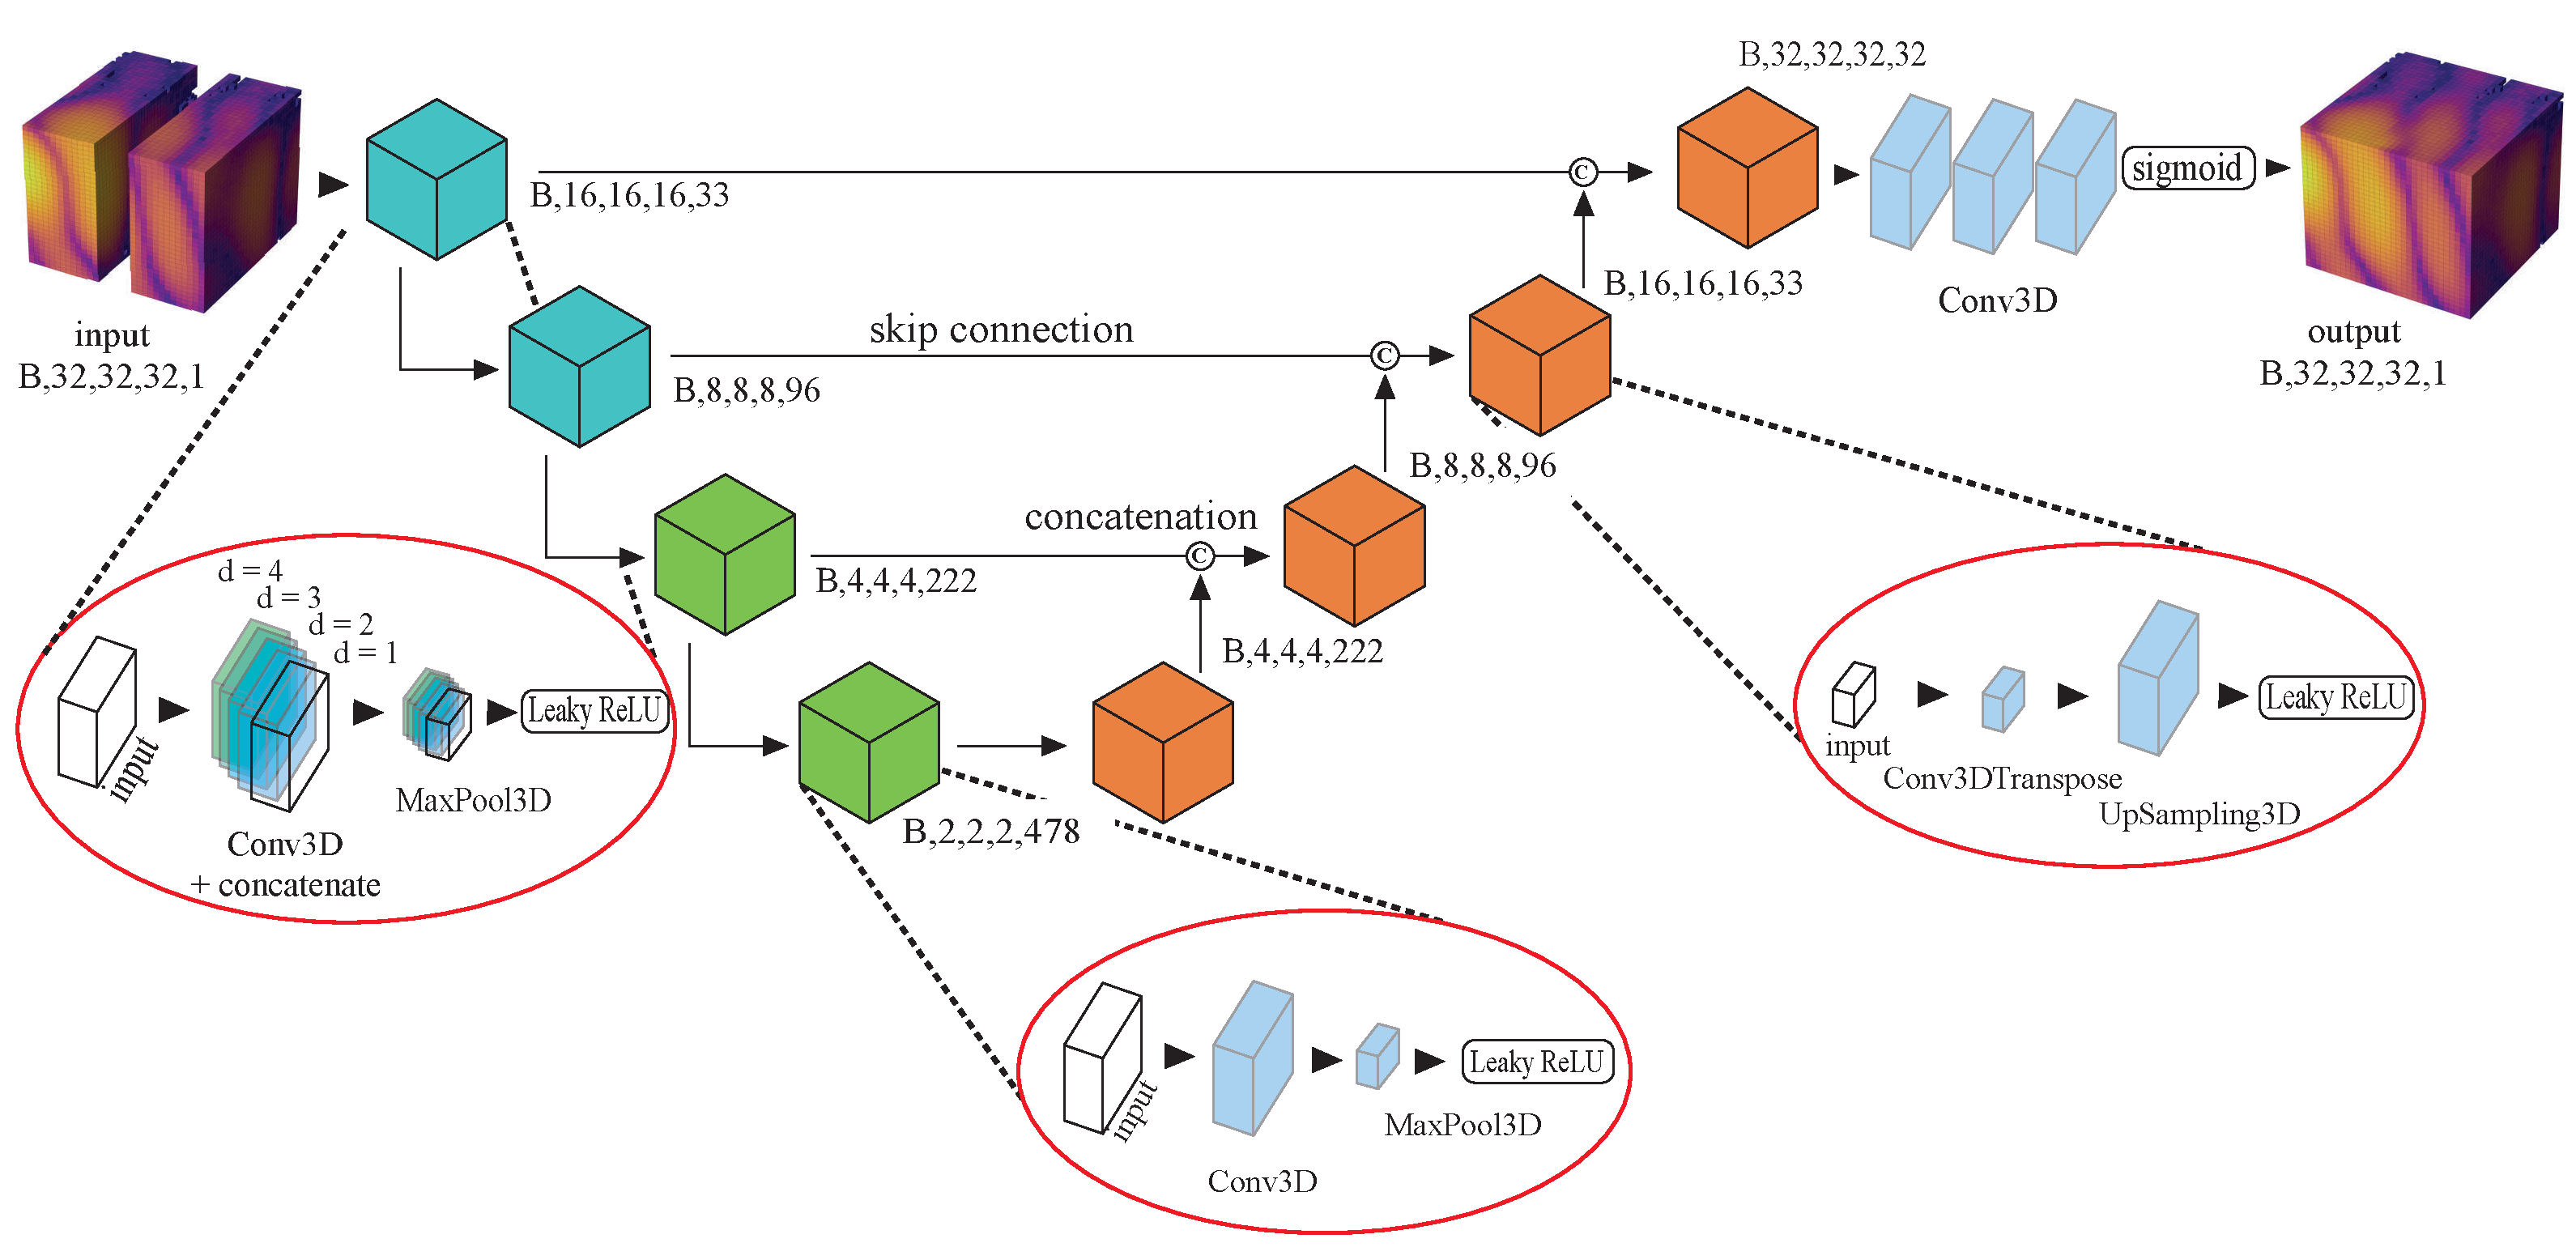
\includegraphics[width=\textwidth]{figures/Inpainting/Architecture_compressed.pdf}
    \caption{\textbf{Schematic of the 3D model architecture} The model uses a modified U-Net structure. 
    In the first two encoder blocks (highlighted by the left red circle), dilated convolutions are applied where the 
    original input is concatenated with its convolutions at various dilation rates (\textit{d = 4,3,2,1}) prior 
    to the MaxPooling operation. The input consists of small gap-affected portions, grouped into batches
     of 32 (B). These portions (top left) are progressively processed by the encoder until they are reduced to a 
     $ 2\times2\times2$ pixel-size feature map. In the decoder, each building block (represented as orange cubes) receives 
     as input the concatenation of the output from the previous block and the matching output from the encoder block 
     of the same size. The final result (top right) is a batch of inpainted versions of the input portions.}

    \label{fig:architecture3d}
\end{figure}

\section{Results in detector space}\label{sec:res_rec}

In this section we will present the results of our DL model on both simulated and experimental diffraction patterns. In
the next section we will move instead to the results in real space, therefore focusing more on the reduction of the artifacts 
in the reconstructed objects.\\

Once completed the training of the model we have first tested it on portions taken from the test dataset. It is possible
to qualitatively observe that the model works equally well for both simulated and experimental data (see Figs. \ref{fig:pred_portions_sim}
- \ref{fig:pred_portions_exp}). From a first visual assessment we can also confirm that low noise regions with larger features
are better restored than others as previously stated in Sec. \ref{sec:performances}. Another curious effect that we can observe, 
is the ``smoothening'' of features around noisy areas (see first column in Fig. \ref{fig:pred_portions_sim} and last column in Fig.
- \ref{fig:pred_portions_exp}). In fact, the ``grainy'' aspect of these regions is caused by Poisson noise which cannot
be predicted by the DL model as it is uncorrelated. In those regions the DL performs therefore a sort of average that 
``smoothens'' the features and acts like a denoiser. This effect has been already studied in the literature and exploited 
for denoising applications like the Noise2Void model \cite{Noise2Void}.

\begin{figure}[h]
    \centering
    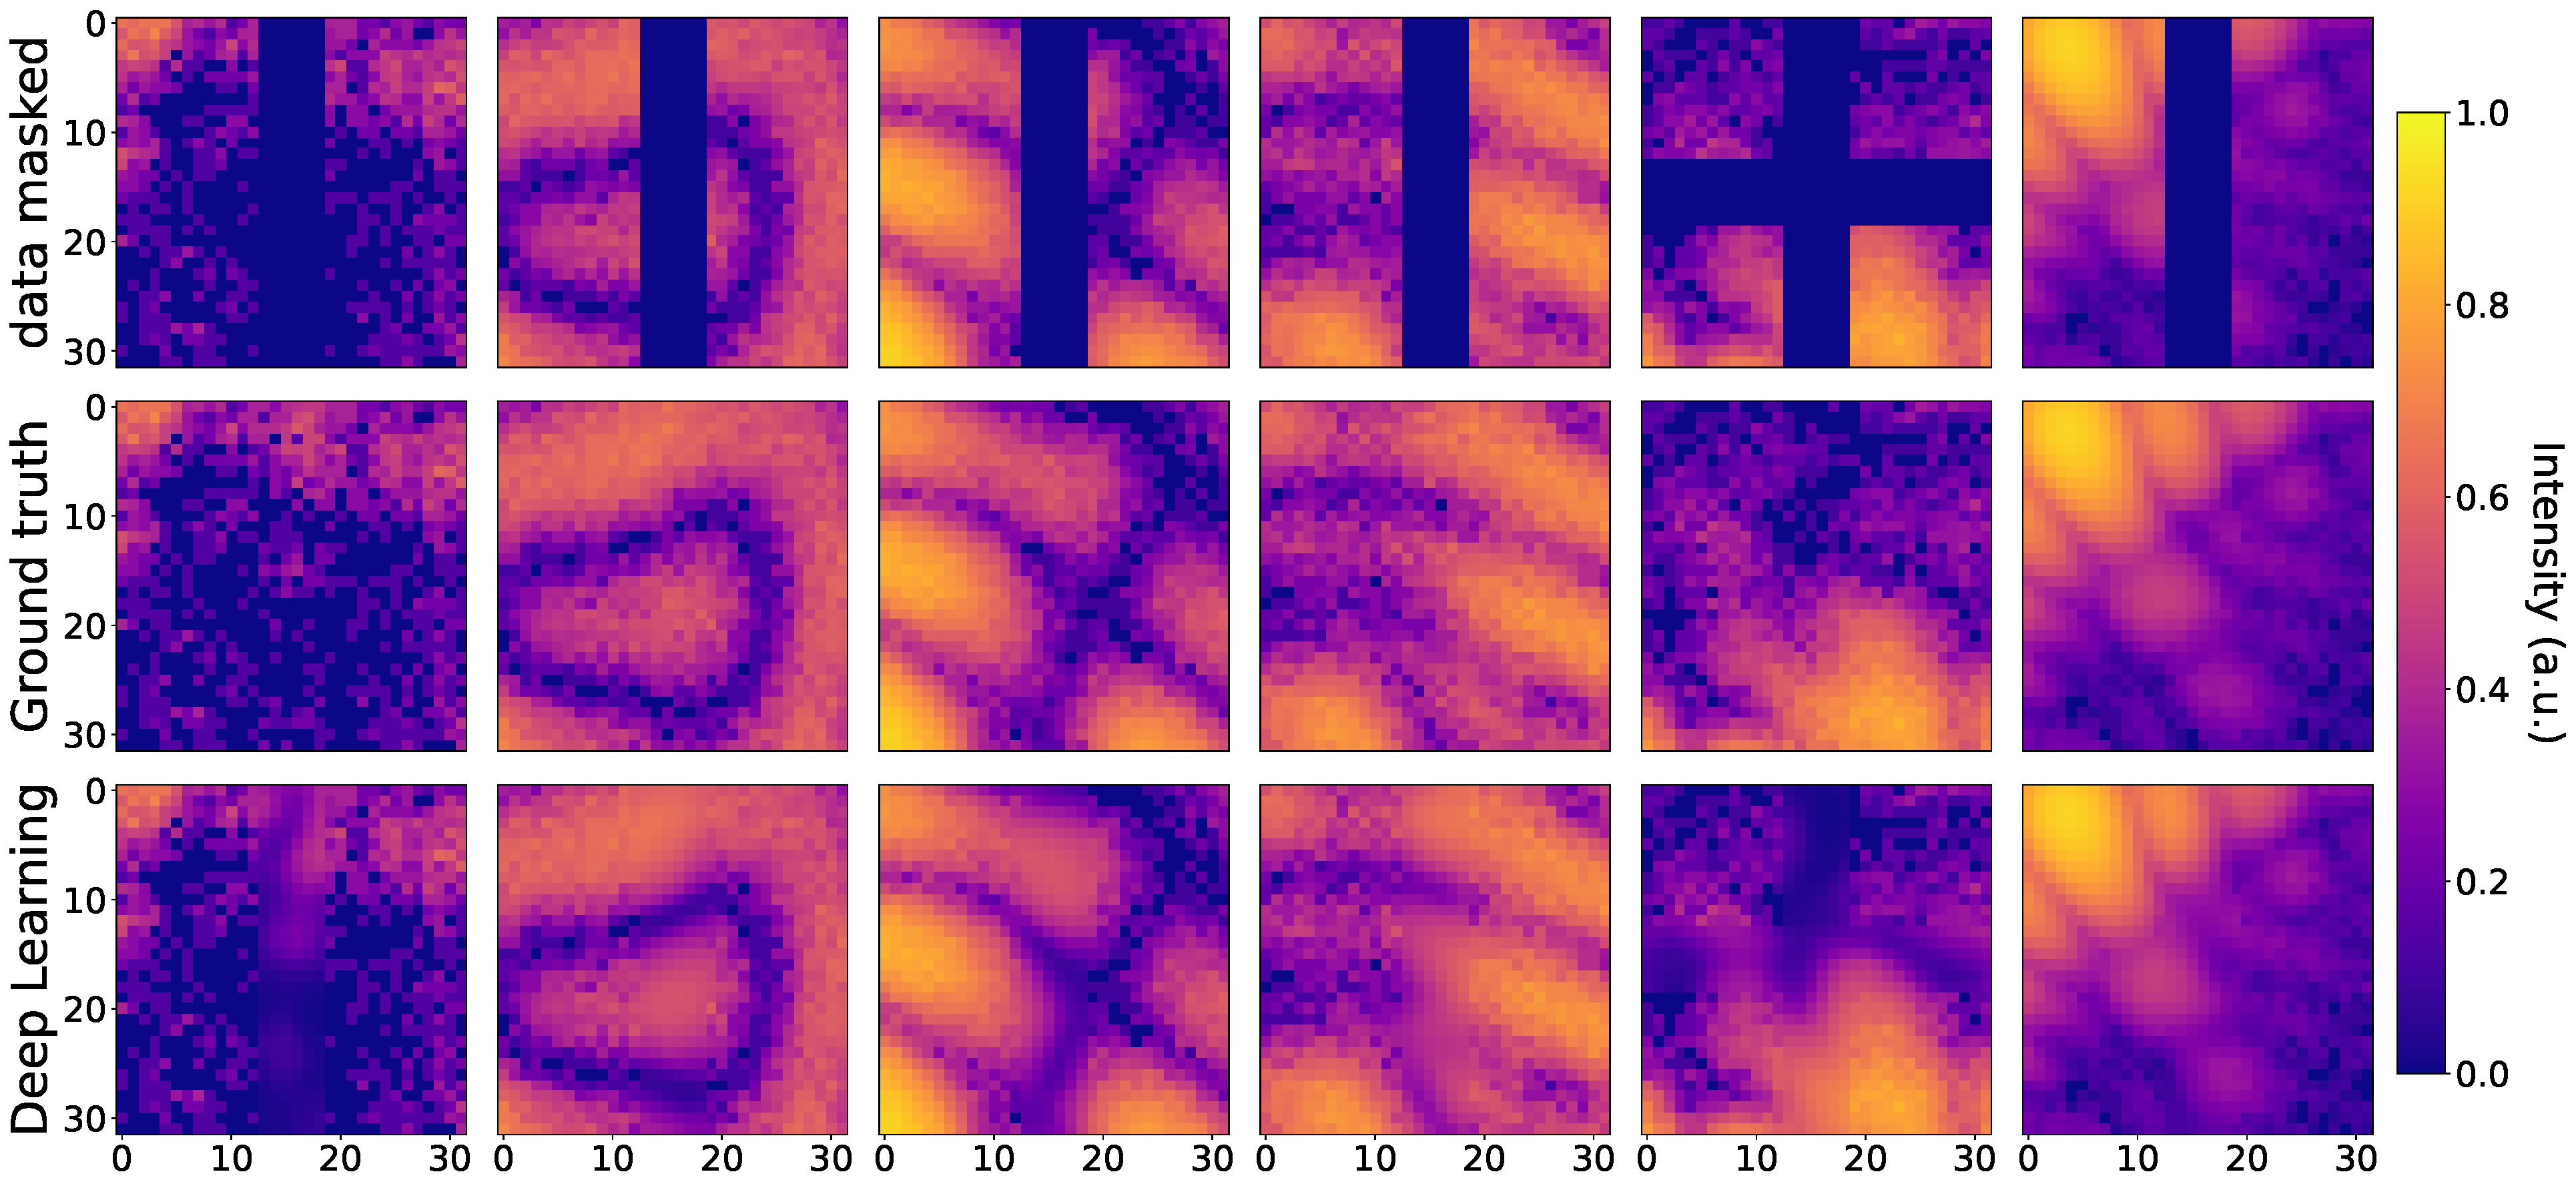
\includegraphics[width=\textwidth]{figures/Inpainting/prediction_small_simulated.pdf}
    \caption{\textbf{Results on portions of test simulated data}. Central slices of portions taken from the simulated test
    dataset. Masked input with 6 pixel-wide gap in the first row, corresponding ground truth and DL inpainted in second and third
    row respectively.}
    \label{fig:pred_portions_sim}
\end{figure}

\begin{figure}[h]
    \centering
    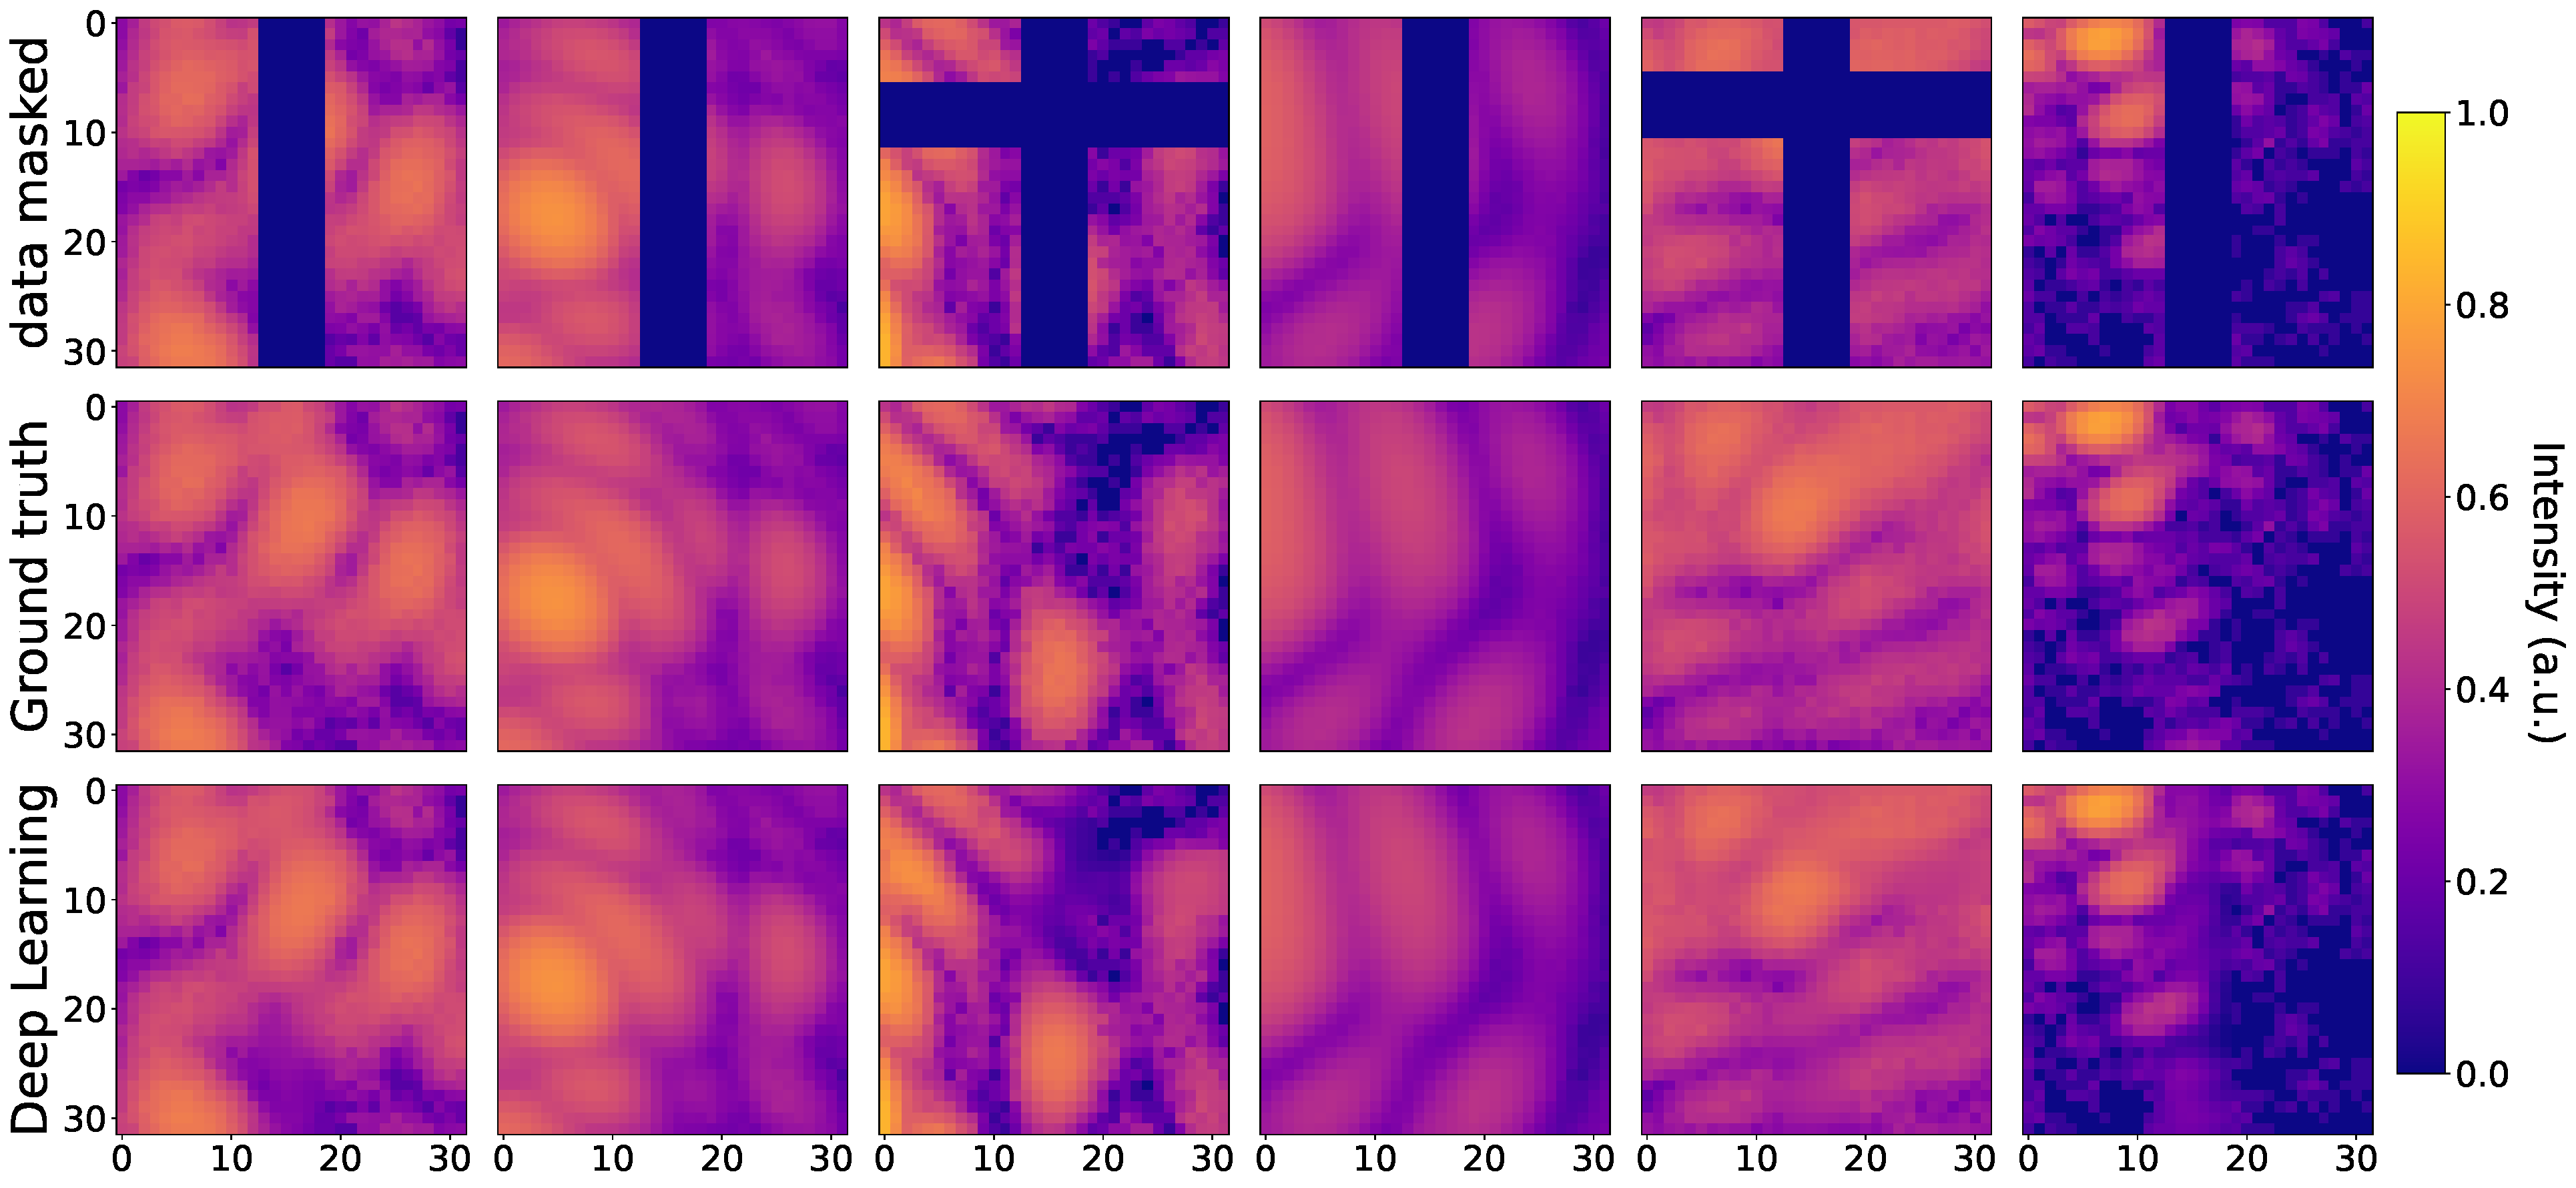
\includegraphics[width=\textwidth]{figures/Inpainting/prediction_small_experiment.pdf}
    \caption{\textbf{Results on portions of test experimental data}. Central slices of portions taken from the experimental test
    dataset. Masked input with 6 pixel-wide gap in the first row, corresponding ground truth and DL inpainted in second and third
    row respectively.}
    \label{fig:pred_portions_exp}
\end{figure}

\subsection{Full gap inpainting}\label{sec:full_gap}

For the inpainting of a gap inside a full 3D BCDI pattern it is sufficient to apply repeatedly the DL model on sub-volumes 
cropped such that the gap plane lies vertical in the center of the array perpendicularly to the third dimension. Each sub-
volume needs to be preprocessed exactly in the same way described above, i.e. transformed into logarithmic scale and 
normalized between 0 and 1. Moreover, it is advised to apply a mask on the gap, to match exactly the gap width the model
has been trained with. 
One can then proceed along the gap moving forward one pixel at the time, compute the inpainted gap and average the prediction
over the overlapping pixels with the previous predictions. By doing this, potential errors are averaged out and the accuracy
of the prediction is maximized. However, for large datasets this can be time-consuming. For example, for a $128\times128\times128$ pixel-size
diffraction pattern with a cross-shaped gap the time needed to compute the full inpainting amounts to 11 minutes (using a 
NVIDIA Tesla V100-SXM2 GPU with 32GB RAM). However, it is possible to increase the step size to significantly reduce the computing
time without affecting excessively the accuracy (see Fig.\ref{fig:skip_figure}). We have proven that the amount of time for the full inpainting follows a power 
law (see Fig. \ref{fig:skip_case}a) and the accuracy starts dropping significantly for more than 5 pixels skipped at the time
(see Fig. \ref{fig:skip_case}b).  

\begin{figure}[H]
    \centering
    \begin{subfigure}{0.45\textwidth} % Adjust width as needed
        \centering
        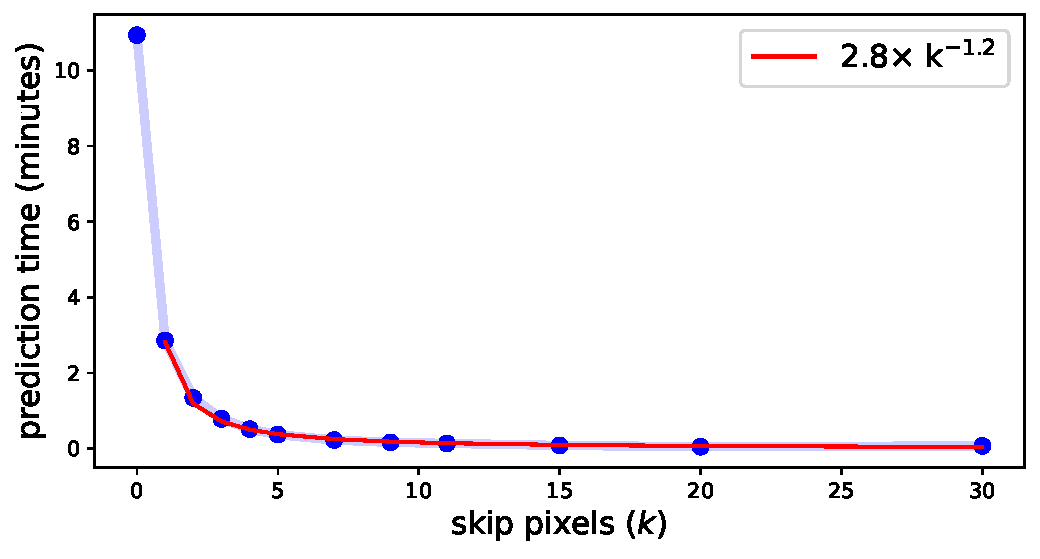
\includegraphics[width=\linewidth]{figures/Inpainting/skip_pixels_time.pdf}
        \caption{\textbf{(a)}}
    \end{subfigure}
    \hfill
    \begin{subfigure}{0.45\textwidth}
        \centering
        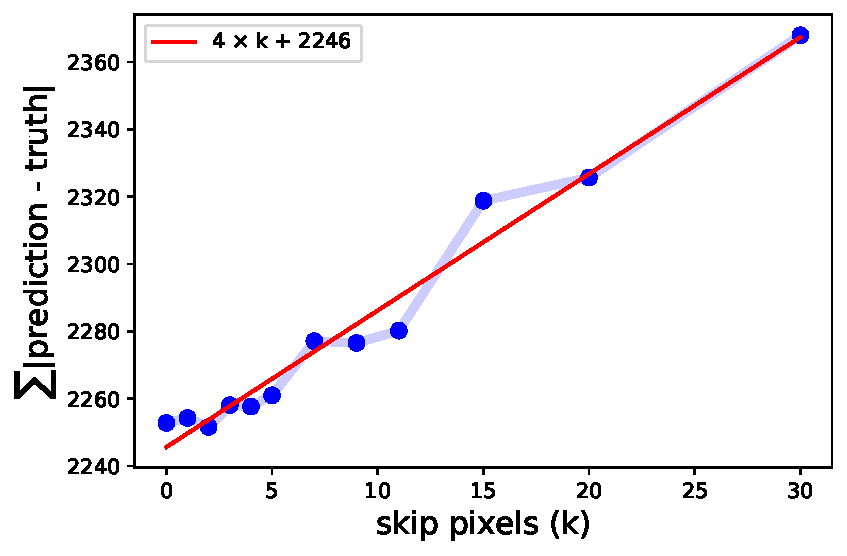
\includegraphics[width=\linewidth]{figures/Inpainting/skip_error.pdf}
        \caption{\textbf{(b)}}
    \end{subfigure}
    \caption{\textbf{(a)} Full inpainting time for a 6 pixel-wide cross-shaped gap on a  $128\times128\times128$ pixel-size
    diffraction pattern as function of the amount of pixels skipped between patch DL predictions along the gap.
    \textbf{(b)} Sum of the absolute errors as function of the skipped pixels. }
    \label{fig:skip_case}
\end{figure}

\begin{figure}[H]
    \centering
    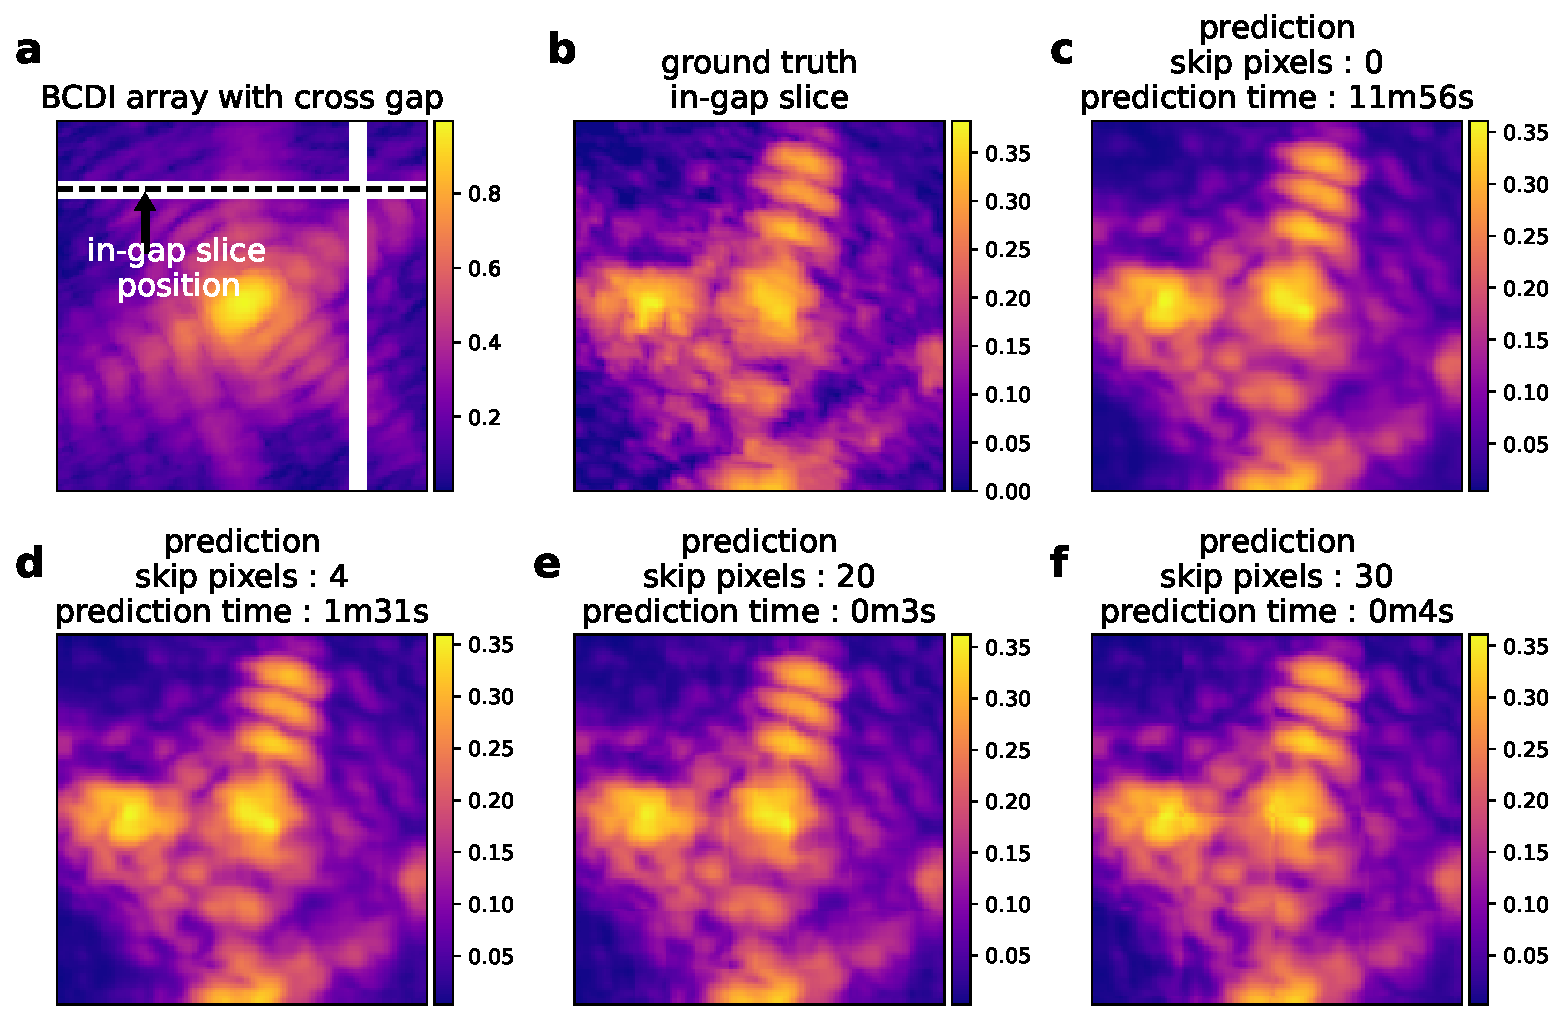
\includegraphics[width=\textwidth]{figures/Inpainting/Skip_pixels_ingap_slice.pdf}
    \caption{Full inpainting of an experimental BCDI pattern for different amounts of skipped pixels. \textbf{a}
    slice of the diffraction pattern perpendicular to the gap plane.\textbf{b} Ground truth intensity inside the gap.
    \textbf{c-d-e-f} In-gap prediction with 0, 4, 20 and 30 skipped pixels respectively, with corresponding 
    execution time. Skipping 4 pixels is a good trade off between time and accuracy.}
    \label{fig:skip_figure}
\end{figure}

\section{Performances assessment}\label{sec:performances}

In order to assess the performances of our DL model with respect to other inpainting methods, we tested it against 
conventional interpolation methods. Specifically, we have taken an experimental BCDI pattern with a 6 pixel-wide 
cross-shaped gap and compared the inpainting results of our DL model with (i) linear interpolation (ii) cubic interpolation 
(iii) nearest-neighbor interpolation. These techniques allow for a quick estimation of the intensity distribution 
inside the gaps but fail to recover fine features (see Figs. \ref{fig:interp}). In particular, we can notice 
in the \textit{in-gap slice} (Fig. \ref{fig:interp}a) that linear interpolation for instance doesn't retrieve correctly 
the space curvature of the fringes while nearest neighbor and cubic interpolations show artifacts in correspondence 
of the perpendicular gap. When considering the central slice perpendicular to the gap planes (along the rocking curve
dimension) we can notice even more how the DL model outperforms conventional interpolations (Fig. \ref{fig:interp}b).
 

\begin{figure}[H]
    \centering
    \begin{subfigure}{0.47\textwidth} 
        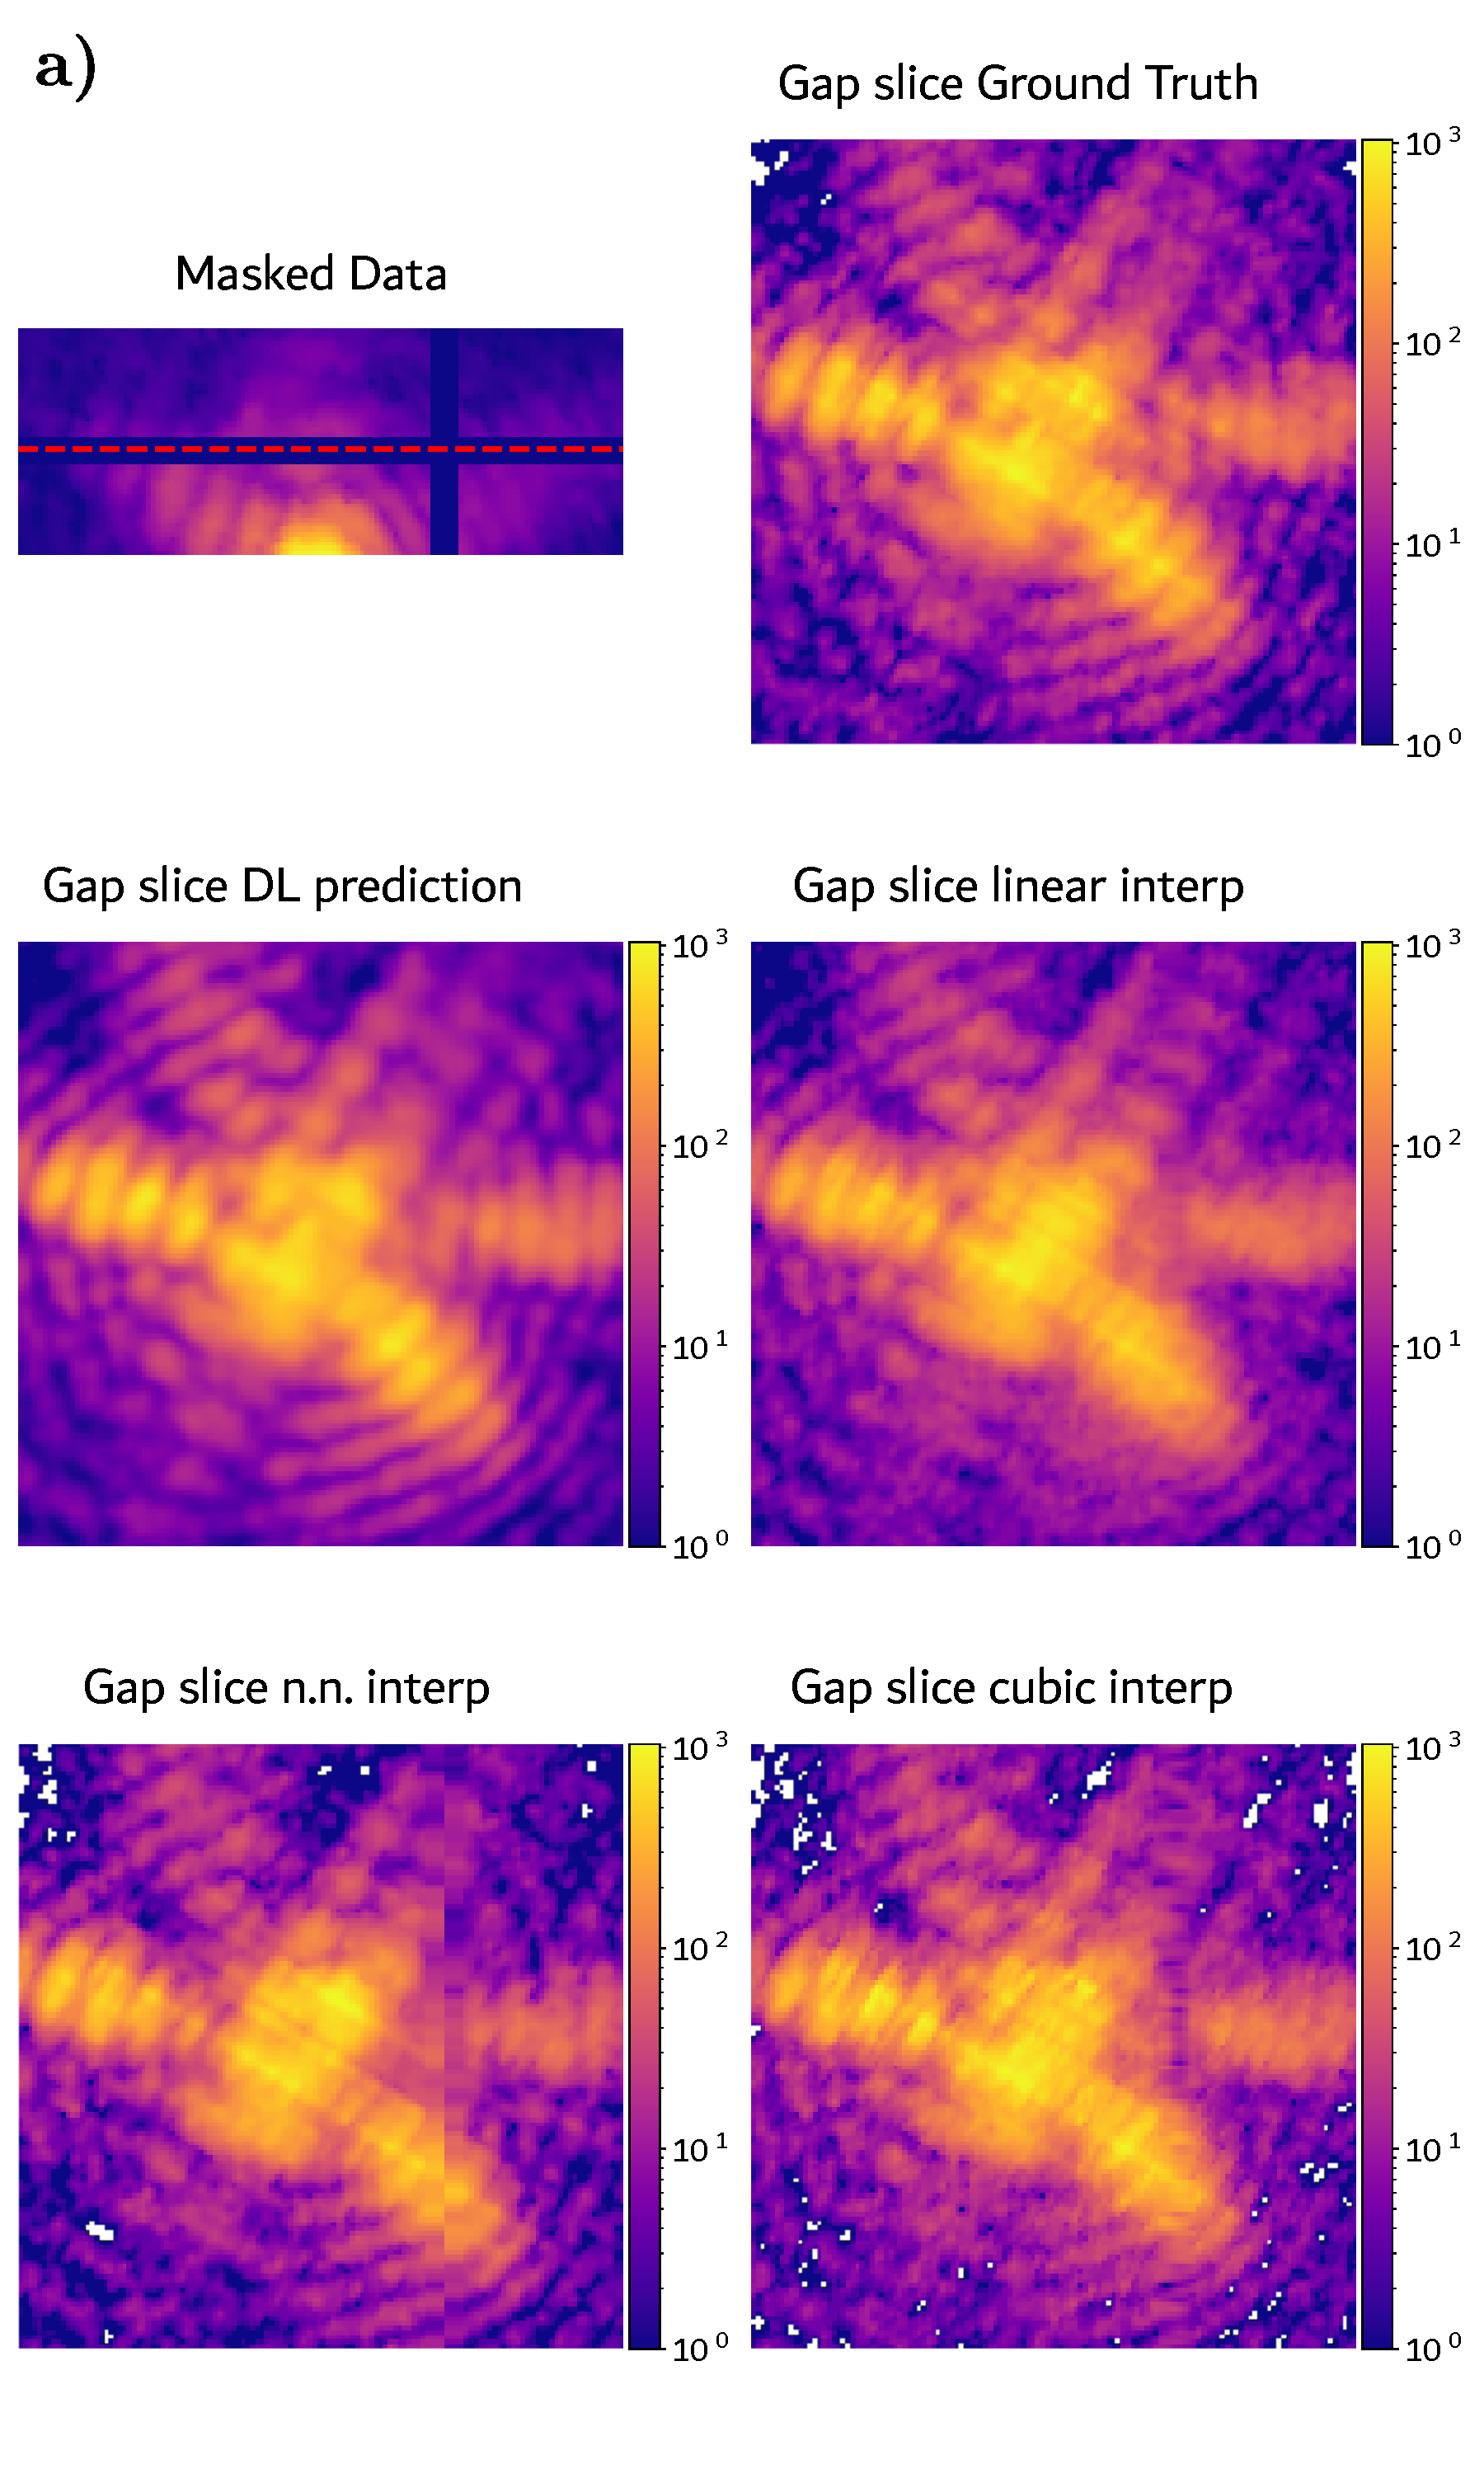
\includegraphics[width=\linewidth]{figures/Inpainting/newfig3_suppl.pdf}
        \caption{\textbf{(a)}}
    \end{subfigure}
    \hfill
    \begin{subfigure}{0.47\textwidth}
        \centering
        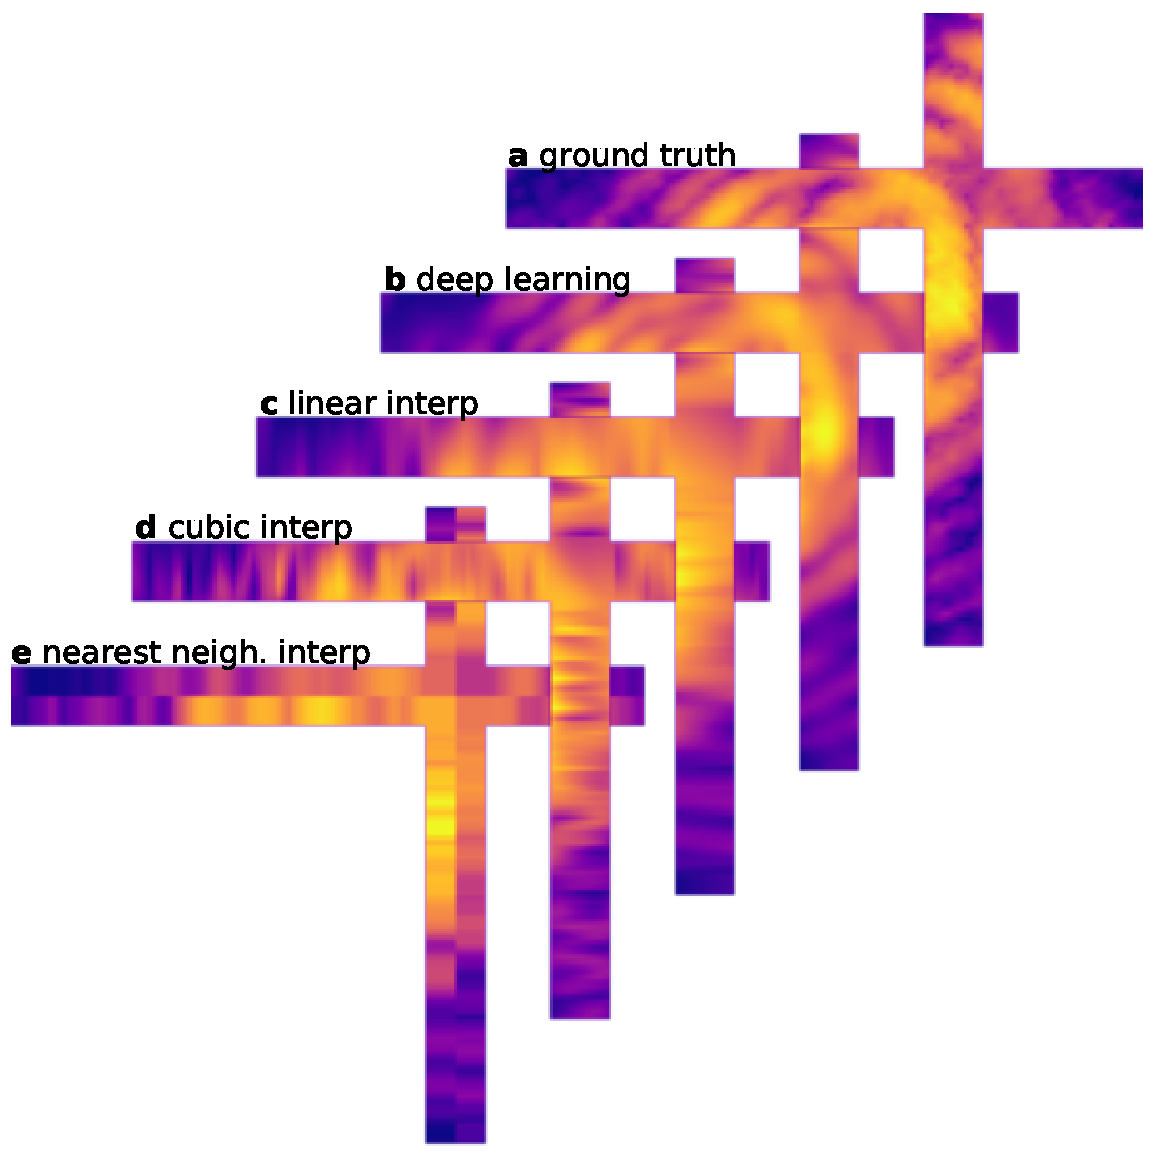
\includegraphics[width=\linewidth]{figures/Inpainting/cross_interp.pdf}
        \caption{\textbf{(b)}}
    \end{subfigure}
    \caption{}
    \label{fig:interp}
\end{figure}


Similarly to the 2D case above, we have also evaluated the performances of the model against the amount of intensity 
inside the sub-volume and against the oversampling ratio. We repeated the test for different gap widths, namely 3,6,9,12 
pixel-wide, using vertical gaps placed in the center of each portion. 
For the first performance assessment we have considered a full simulated $128\times128\times128$ pixel-size BCDI pattern
and randomly cropped out of it 1000 portions. We have then applied a vertical gap in the center of each portion for different 
gap sizes and then computed the prediction with the corresponding DL model. The intensity (in pixel counts) inside each sub-
volume was then summed and the obtained values for the 1000 samples were binned into 20 classes for better visualization. 
The accuracy scores, calculated with the PCC, were then averaged inside each bin class. The results are displayed in Fig. 
\ref{fig:acc_int_3D}. As expected from what discussed above for the 2D case, better accuracy scores are obtained for portions
containing larger amount of signals, where noise levels are lower and the features of the diffraction pattern are more 
visible. Moreover, the plot logically shows that smaller gaps are generally better recovered, but it is worth noticing
that the accuracy spread across different gap sizes widens for noisy portions and narrows down as the amount of signal 
increases. These trends suggest that DL models are overall robust to different gap sizes especially for high intensity regions, 
which are eventually the most important ones as they contribute the most during to the reconstruction. 

\begin{figure}[H]
    \centering
    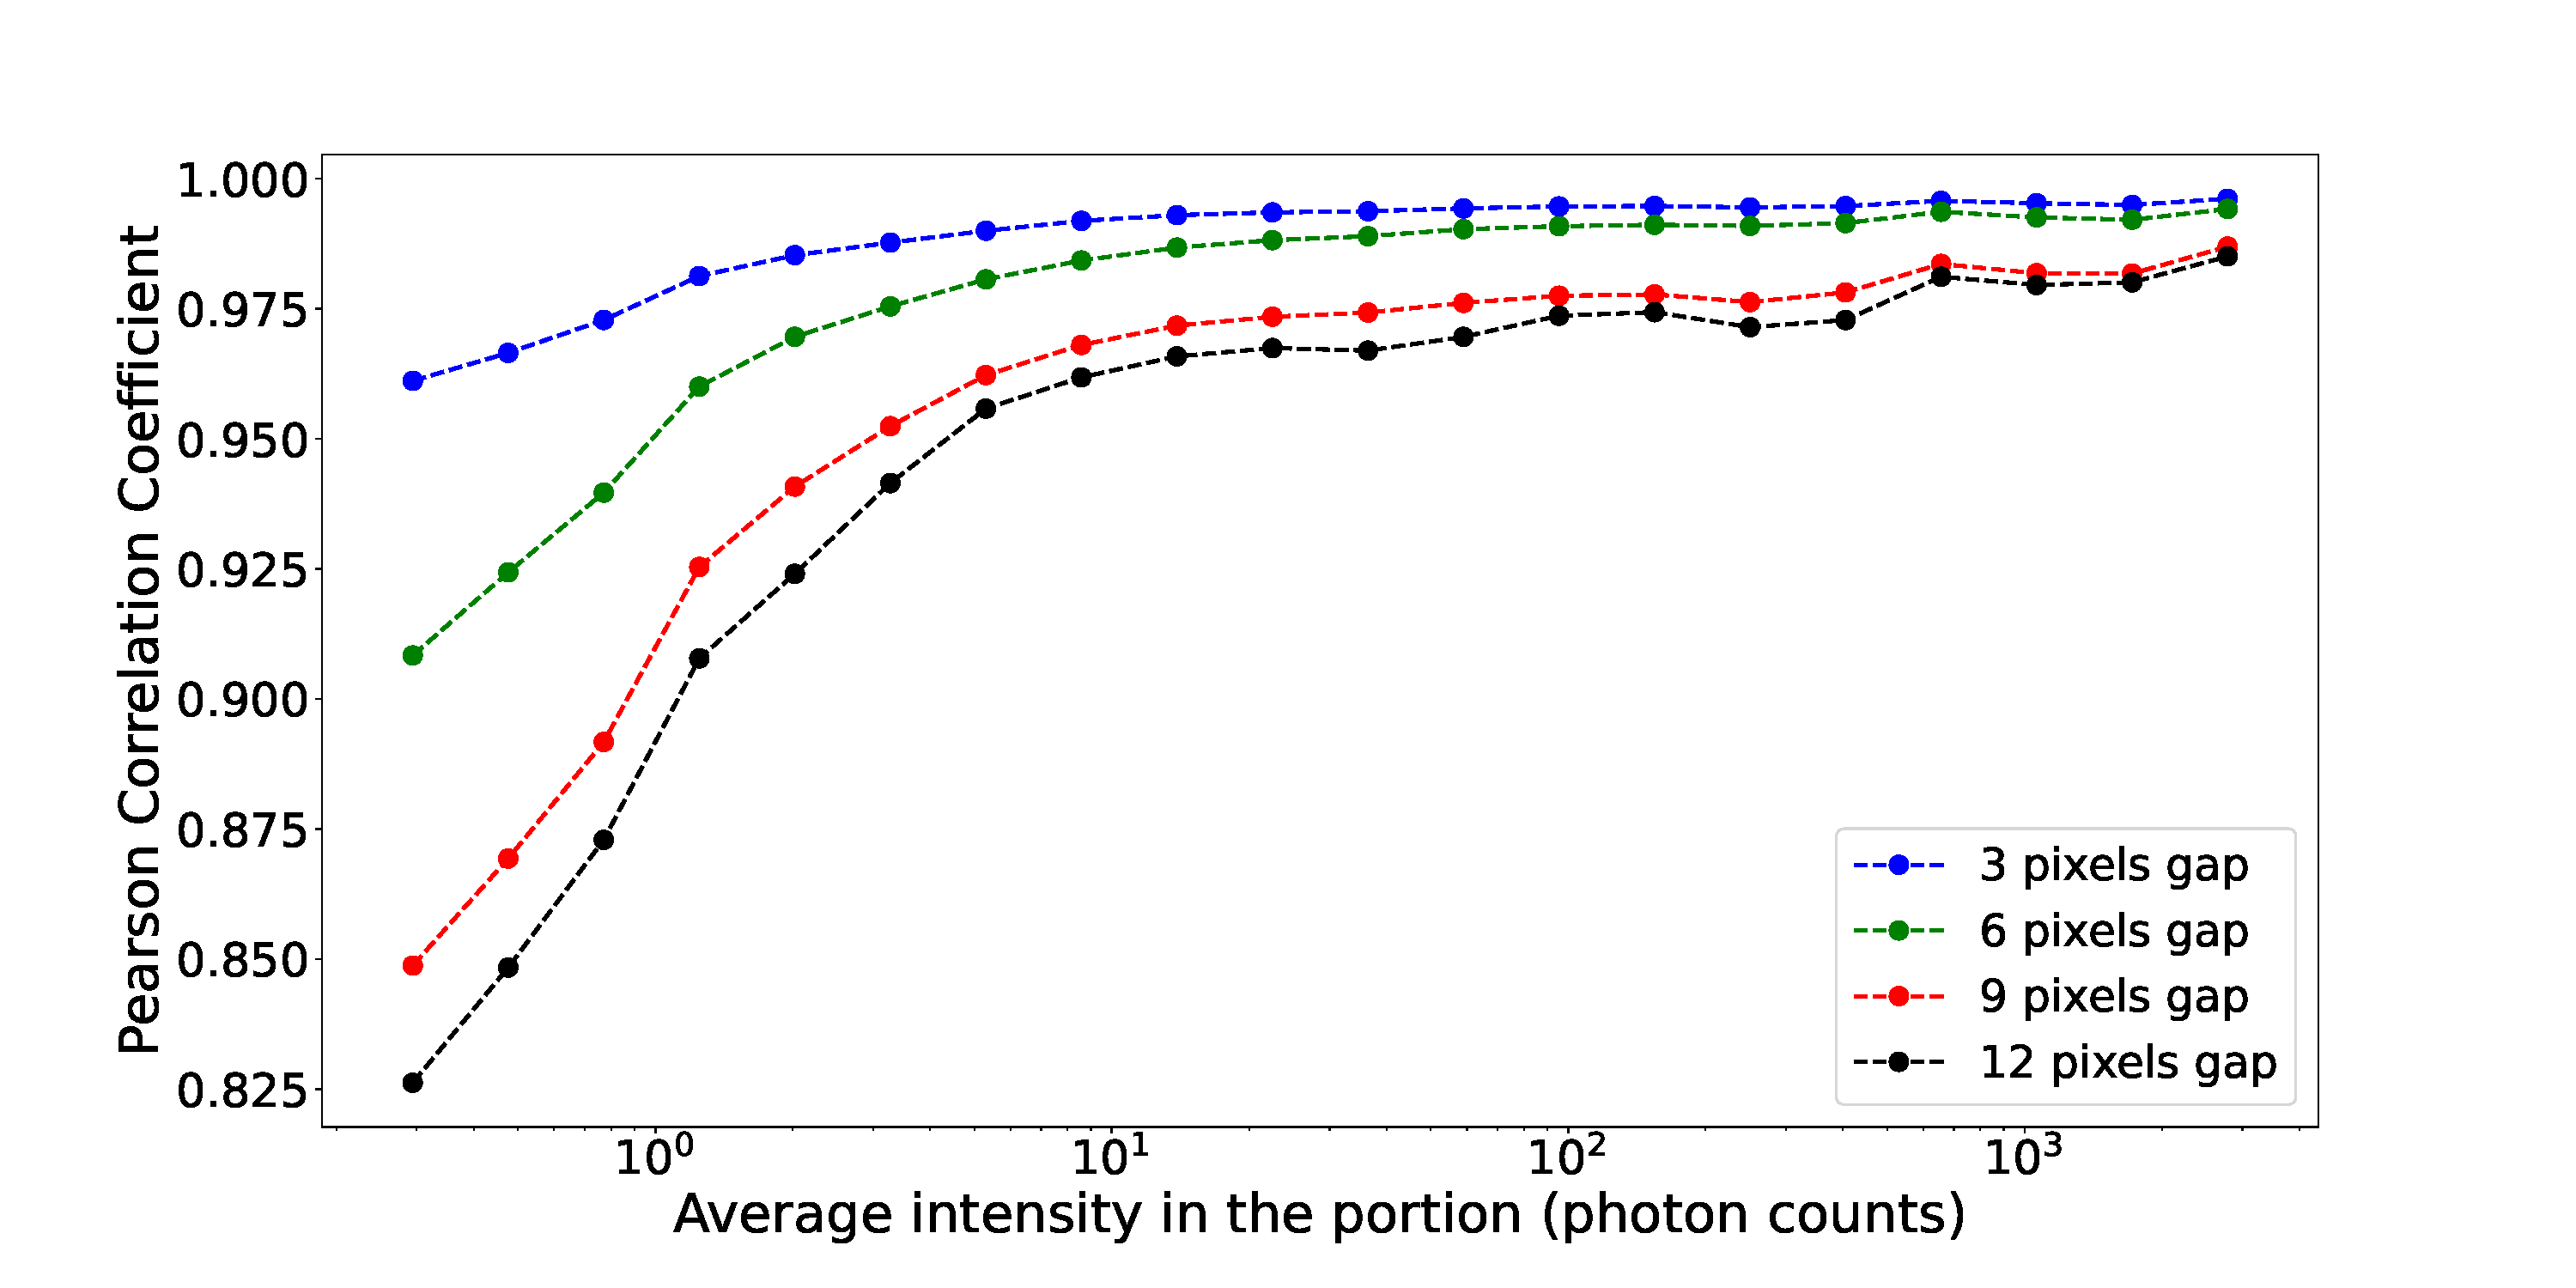
\includegraphics[width=\textwidth]{figures/Inpainting/1D_Acc_Intensity.pdf}
    \caption{Accuracy scores (PCC) of the DL patching model }
    \label{fig:acc_int_3D}
\end{figure}

The last test concerns the study of the accuracy for different oversampling ratios. As anticipated above for the 2D case, 
to carry out properly this evaluation, one should consider the same diffraction pattern extending to the same equivalent
$Q$-space value for each oversampling ratio. This in practice is done reducing increasing the $dq$ per pixel as decreasing
the oversampling ratio, resulting in a smaller size of the overall BCDI pattern. In our particular case we have simulated
the same BCDI pattern for oversampling ratios spanning from 2 to 7. For each oversampling ratio, a vertical gap
mask was applied to the whole BCDI array and the DL prediction was calculated with no-skip pixel (see Sec. \ref{sec:full_gap}).
The gap was then shifted laterally and this procedure was repeated until the whole BCDI array was predicted using our
model, thus leading to a full BCDI predicted image. The PCC was then calculated using the whole BCDI array for 
different oversampling ratios and model gap sizes. The results are displayed in Fig. \ref{fig:acc_ovs_3D}. As expected,
the predictions are more accurate for large oversampling ratios and small gap sizes (i.e., large oscillation periods 
relative to the gap width). 

\begin{figure}[H]
    \centering
    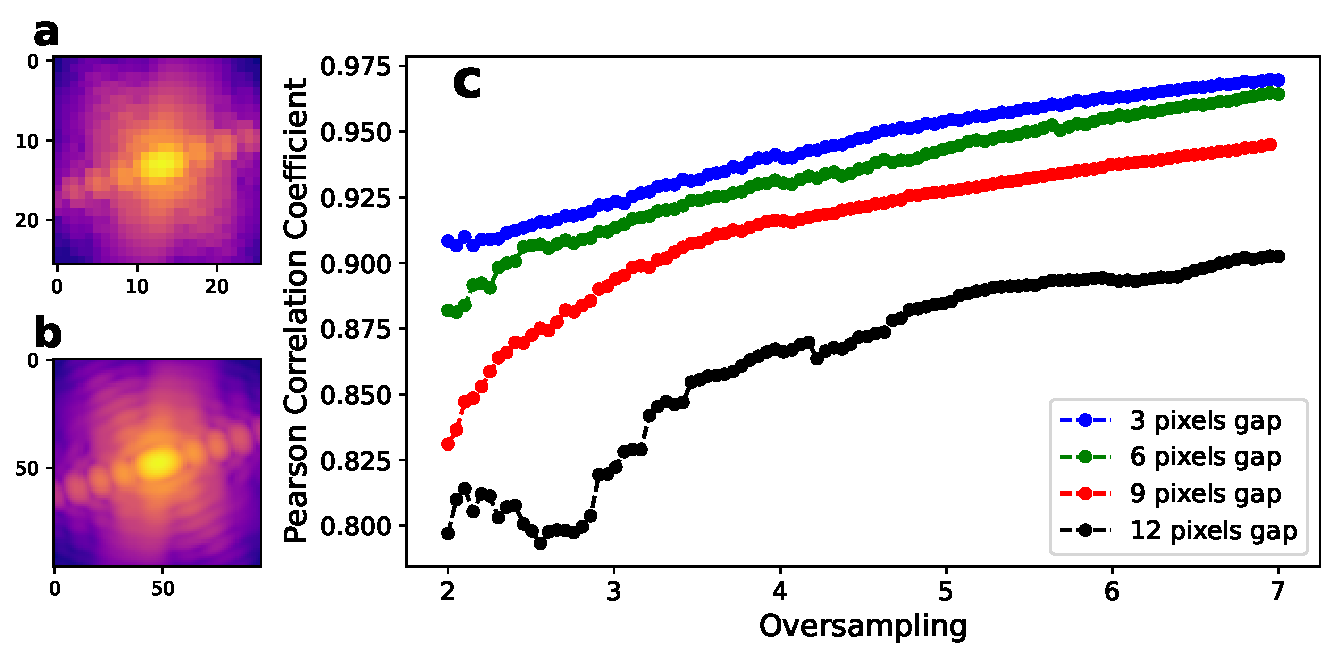
\includegraphics[width=\textwidth]{figures/Inpainting/accuracy_oversampling.pdf}
    \caption{Accuracy scores (PCC) of the DL patching model against the oversampling ratio. }
    \label{fig:acc_ovs_3D}
\end{figure}

\section{Results in real space}\label{sec:res_real}

In this section we will discuss the effects of DL inpainting on the reconstructed objects for both simulated and experimental 
data. In particular, we will assess, both qualitatively and quantitatively, the gap induced artifacts in 
the modulus, phase and strain fields of the reconstructions and their reduction thanks to the DL inpainting. To carry out
these analyses we have taken an experimental BCDI dataset acquired at the ID01 beamline of the ESRF and already exploited by 
Carnis \textit{et al.} in 2019 for similar studies on gap-induced artifacts \cite{carnis_towards_2019}. The dataset 
corresponds to the BCDI pattern around the (\textbf{111}) peak of a Pt tetrahextrahedral (THH) particle (400 nm in size). 
Similarly to what the authors did, we have kept the modulus of the reconstructed object and set the real space phase
to zero, making it our reference ground-truth object $\textbf{O}$. This measure helps us to highlighting the gap induced artifacts on the phase and strain fields as we have a zero-phase 
reference to compare the results with. We have then calculated the corresponding diffraction pattern with the fast 
Fourier transform (FFT) obtaining a complex diffracted amplitude $\textbf{A}=FFT(\textbf{O})$. A cross-shaped gap was 
subsequently applied to $\textbf{A}$ and the corresponding object $\textbf{O}_{gap}$ was calculated with the inverse FFT.
From the same gapped $\textbf{A}$, the intensity $\textbf{I} = |\textbf{A}|^2$ was also ``inpainted'' using our DL model and corresponding object $\textbf{O}_{DL}$ was 
calculated with the inverse FFT as well, using the ground truth reciprocal space phase. We have repeated the procedure for four different gap sizes (3, 6, 9, 12 px-wide)
matching exactly the cases mentioned in the work of Carnis and coauthors. Figure Fig.\ref{fig:Carnis_int} shows the projection
along the rocking curve axis (XY slice in this case) of the ground truth diffracted intensity, the gapped and the DL inpainted ones for the 
9 pixel-wide gap case.

\begin{figure}[H]
    \centering
    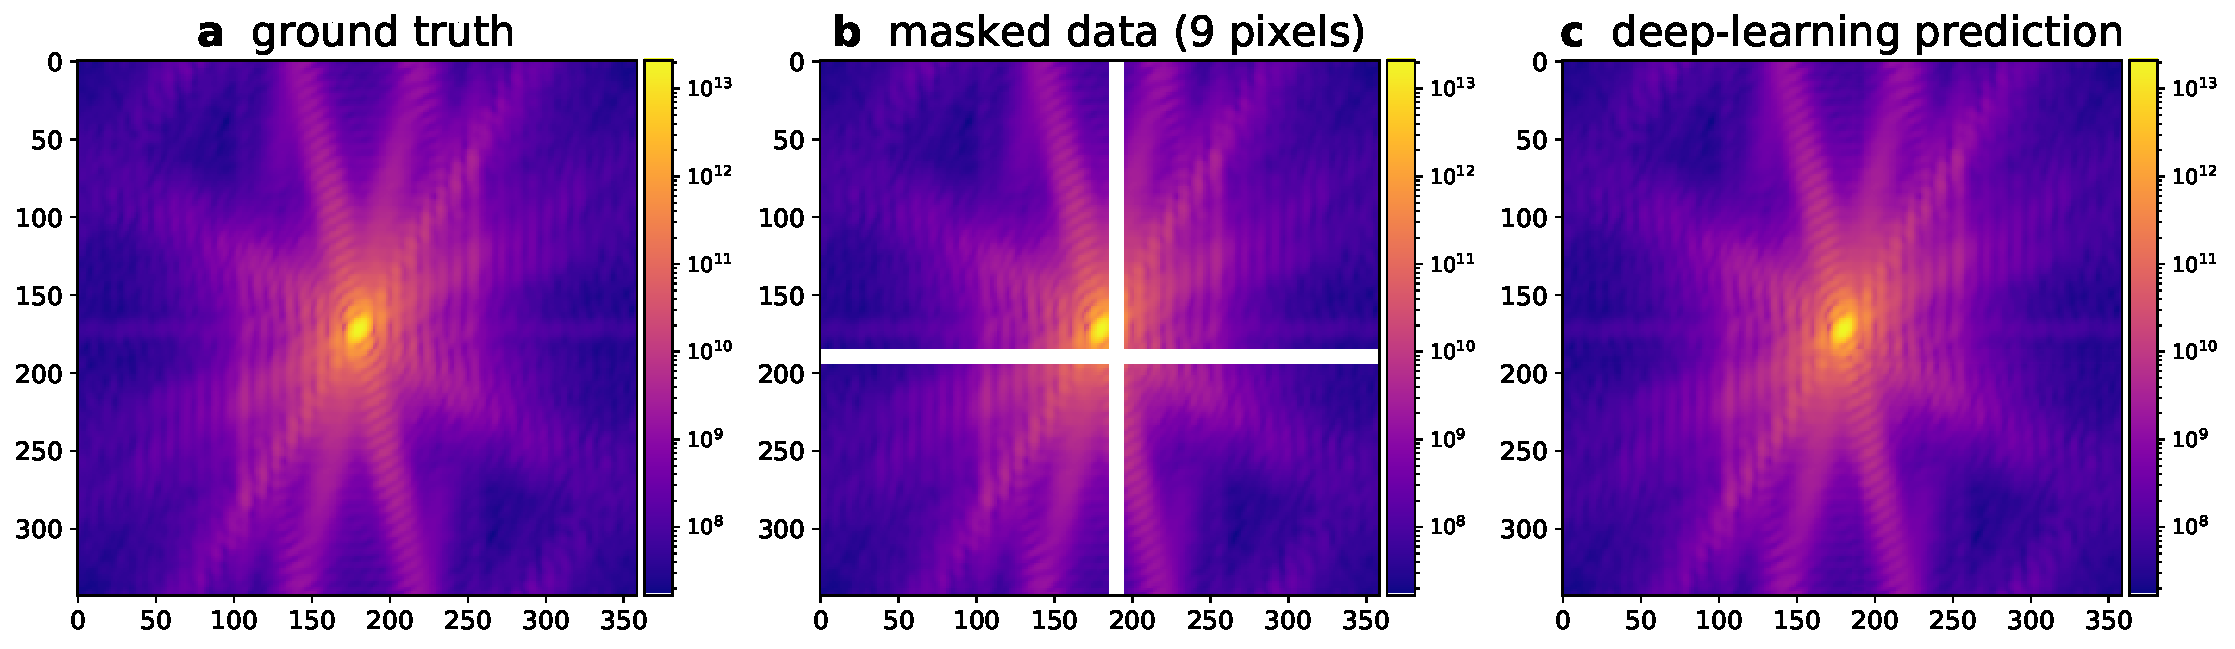
\includegraphics[width=\textwidth]{figures/Inpainting/Carnis_Diffractions_comparison_9px_version2.pdf}
    \caption{\textbf{Projections along the rocking curve axis of the studied diffraction pattern in log scale.} \textbf{a} Ground truth
    pattern obtained from the $|FFT(\textbf{O})|^2$. \textbf{b} Pattern with a 9 pixel-wide cross shaped gap. The position close to the center of 
    the peak is experimentally unlikely but here it allows us to enhance the artifacts in the reconstructions. \textbf{c} 
    Corresponding DL inpainted BCDI pattern. It is visible the presence of aliasing due to the FFT calculation rather than 
    the more correct kinematic sum. This effect is however not relevant for the scope of these analyses.}
    \label{fig:Carnis_int}
\end{figure}

\begin{figure}[H]
    \centering
    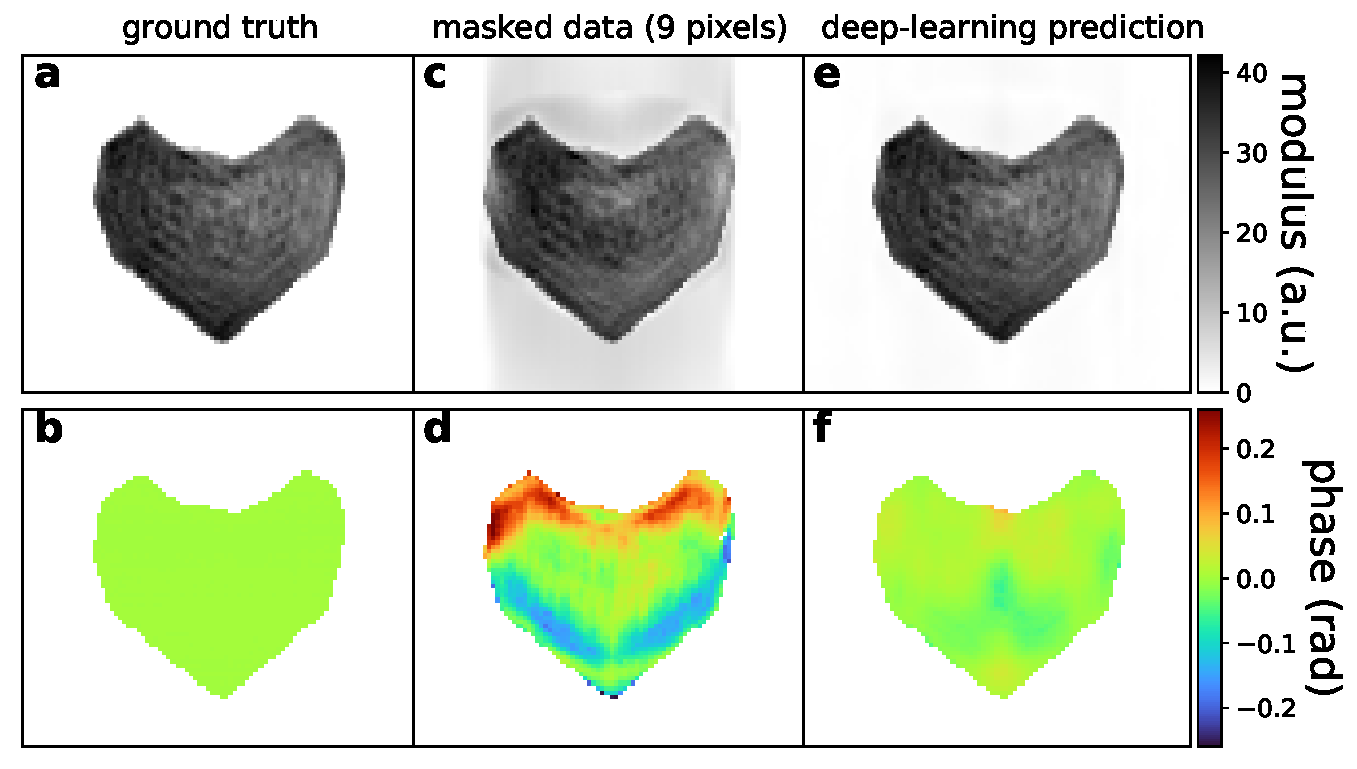
\includegraphics[width=\textwidth]{figures/Inpainting/Real_space_comparison_axis0-1.pdf}
    \caption{\textbf{Reconstructed objects}.\textbf{a-b} Ground truth modulus and phase. \textbf{c-d} Modulus and phase of  
    $\textbf{O}_{gap}$. \textbf{e-f} Modulus and phase of $\textbf{O}_{DL}$}
    \label{fig:Carnis_obj}
\end{figure} 

Figure Fig.\ref{fig:Carnis_obj} illustrate instead the central (YZ) slice of the reconstructed objects for 
the three cases. It is evident that while $\textbf{O}_{gap}$ shows significant abnormalities in both modulus and phase, 
$\textbf{O}_{DL}$ is much closer to the ground truth. In particular one can notice that the gap plane, horizontal in the 
YZ plane, induces artifacts along its perpendicular direction. The result is indeed a stripe of non-zero modulus outside 
the support and, most importantly, an overall phase variation of 0.4 radians along the vertical direction. This phase variation
results in an error of +-7 pm in the lattice displacement field for the 111 Pt reflection, with more intensity around the 
surface. These artefacts are particularly problematic in the cases of (electro-)catalytic experiments \cite{atlan_imaging_2023}
or in situ gas experiments \cite{Ulvestad2015}; Kim et al., 2018; Abuin et al., 2019; Kawaguchi et al., 2019; Dupraz et al., 2022), 
where the chemical reactions occur at the nanoparticle's surfaces and can be studied by following the strain evolution in these
regions. As one could expect the artifacts become more severe as the gap size increases. Fig.\ref{fig:Carnis_allgaps} depicts 
the phases of $\textbf{O}_{gap}$ and $\textbf{O}_{DL}$ for the different gap sizes considered in this study while 
Fig.\ref{fig:Carnis_allgaps_strain} the strain distribution in the XY plane. 

\begin{figure}[H]
    \centering
    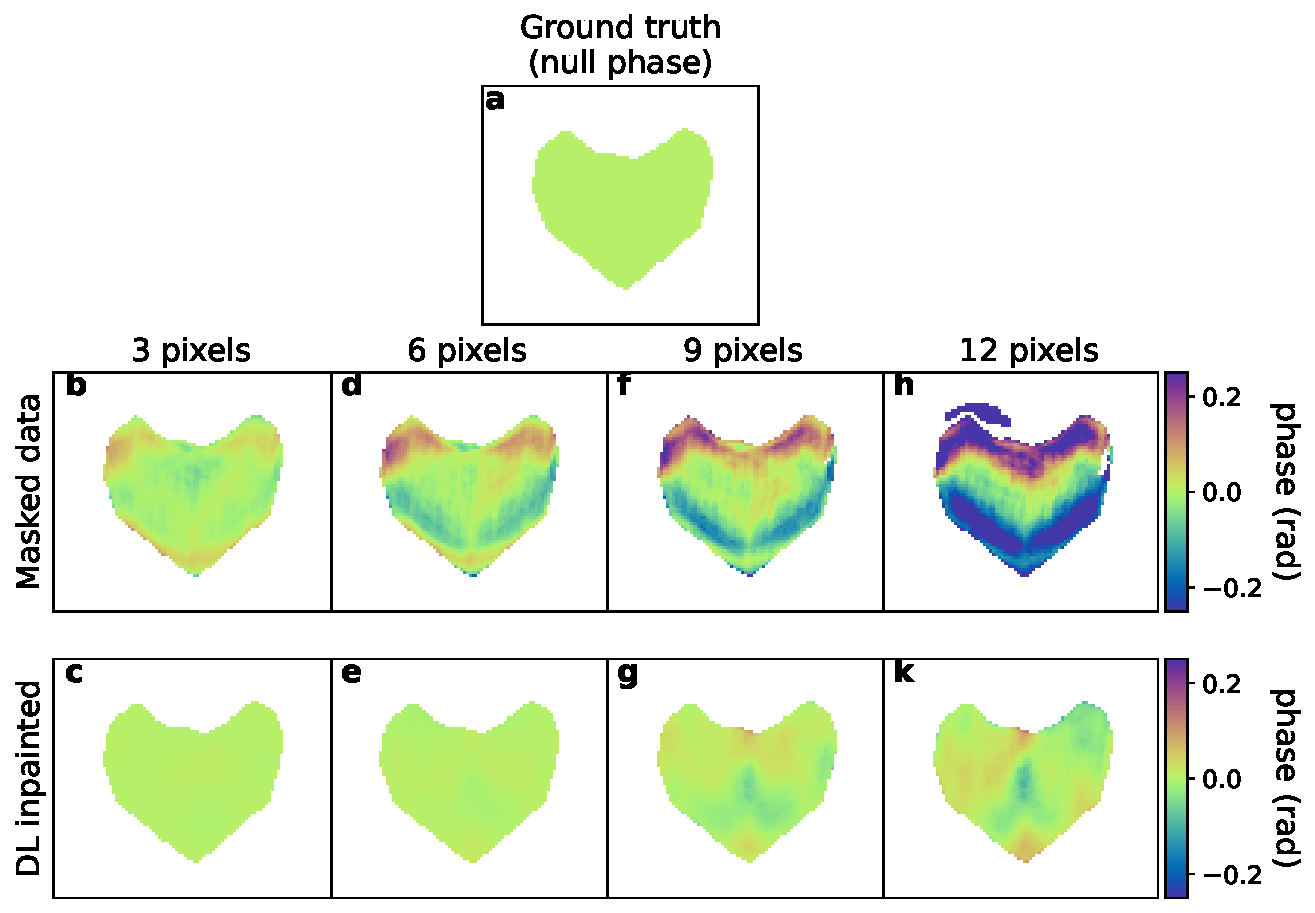
\includegraphics[width=\textwidth]{figures/Inpainting/strain_comparison_allGaps-1.pdf}
    \caption{Artifacts on the phase of $\textbf{O}_{gap}$ for different gap sizes, and phases of the corresponding $\textbf{O}_{DL}$  }
    \label{fig:Carnis_allgaps}
\end{figure}


\begin{figure}[H]
    \centering
    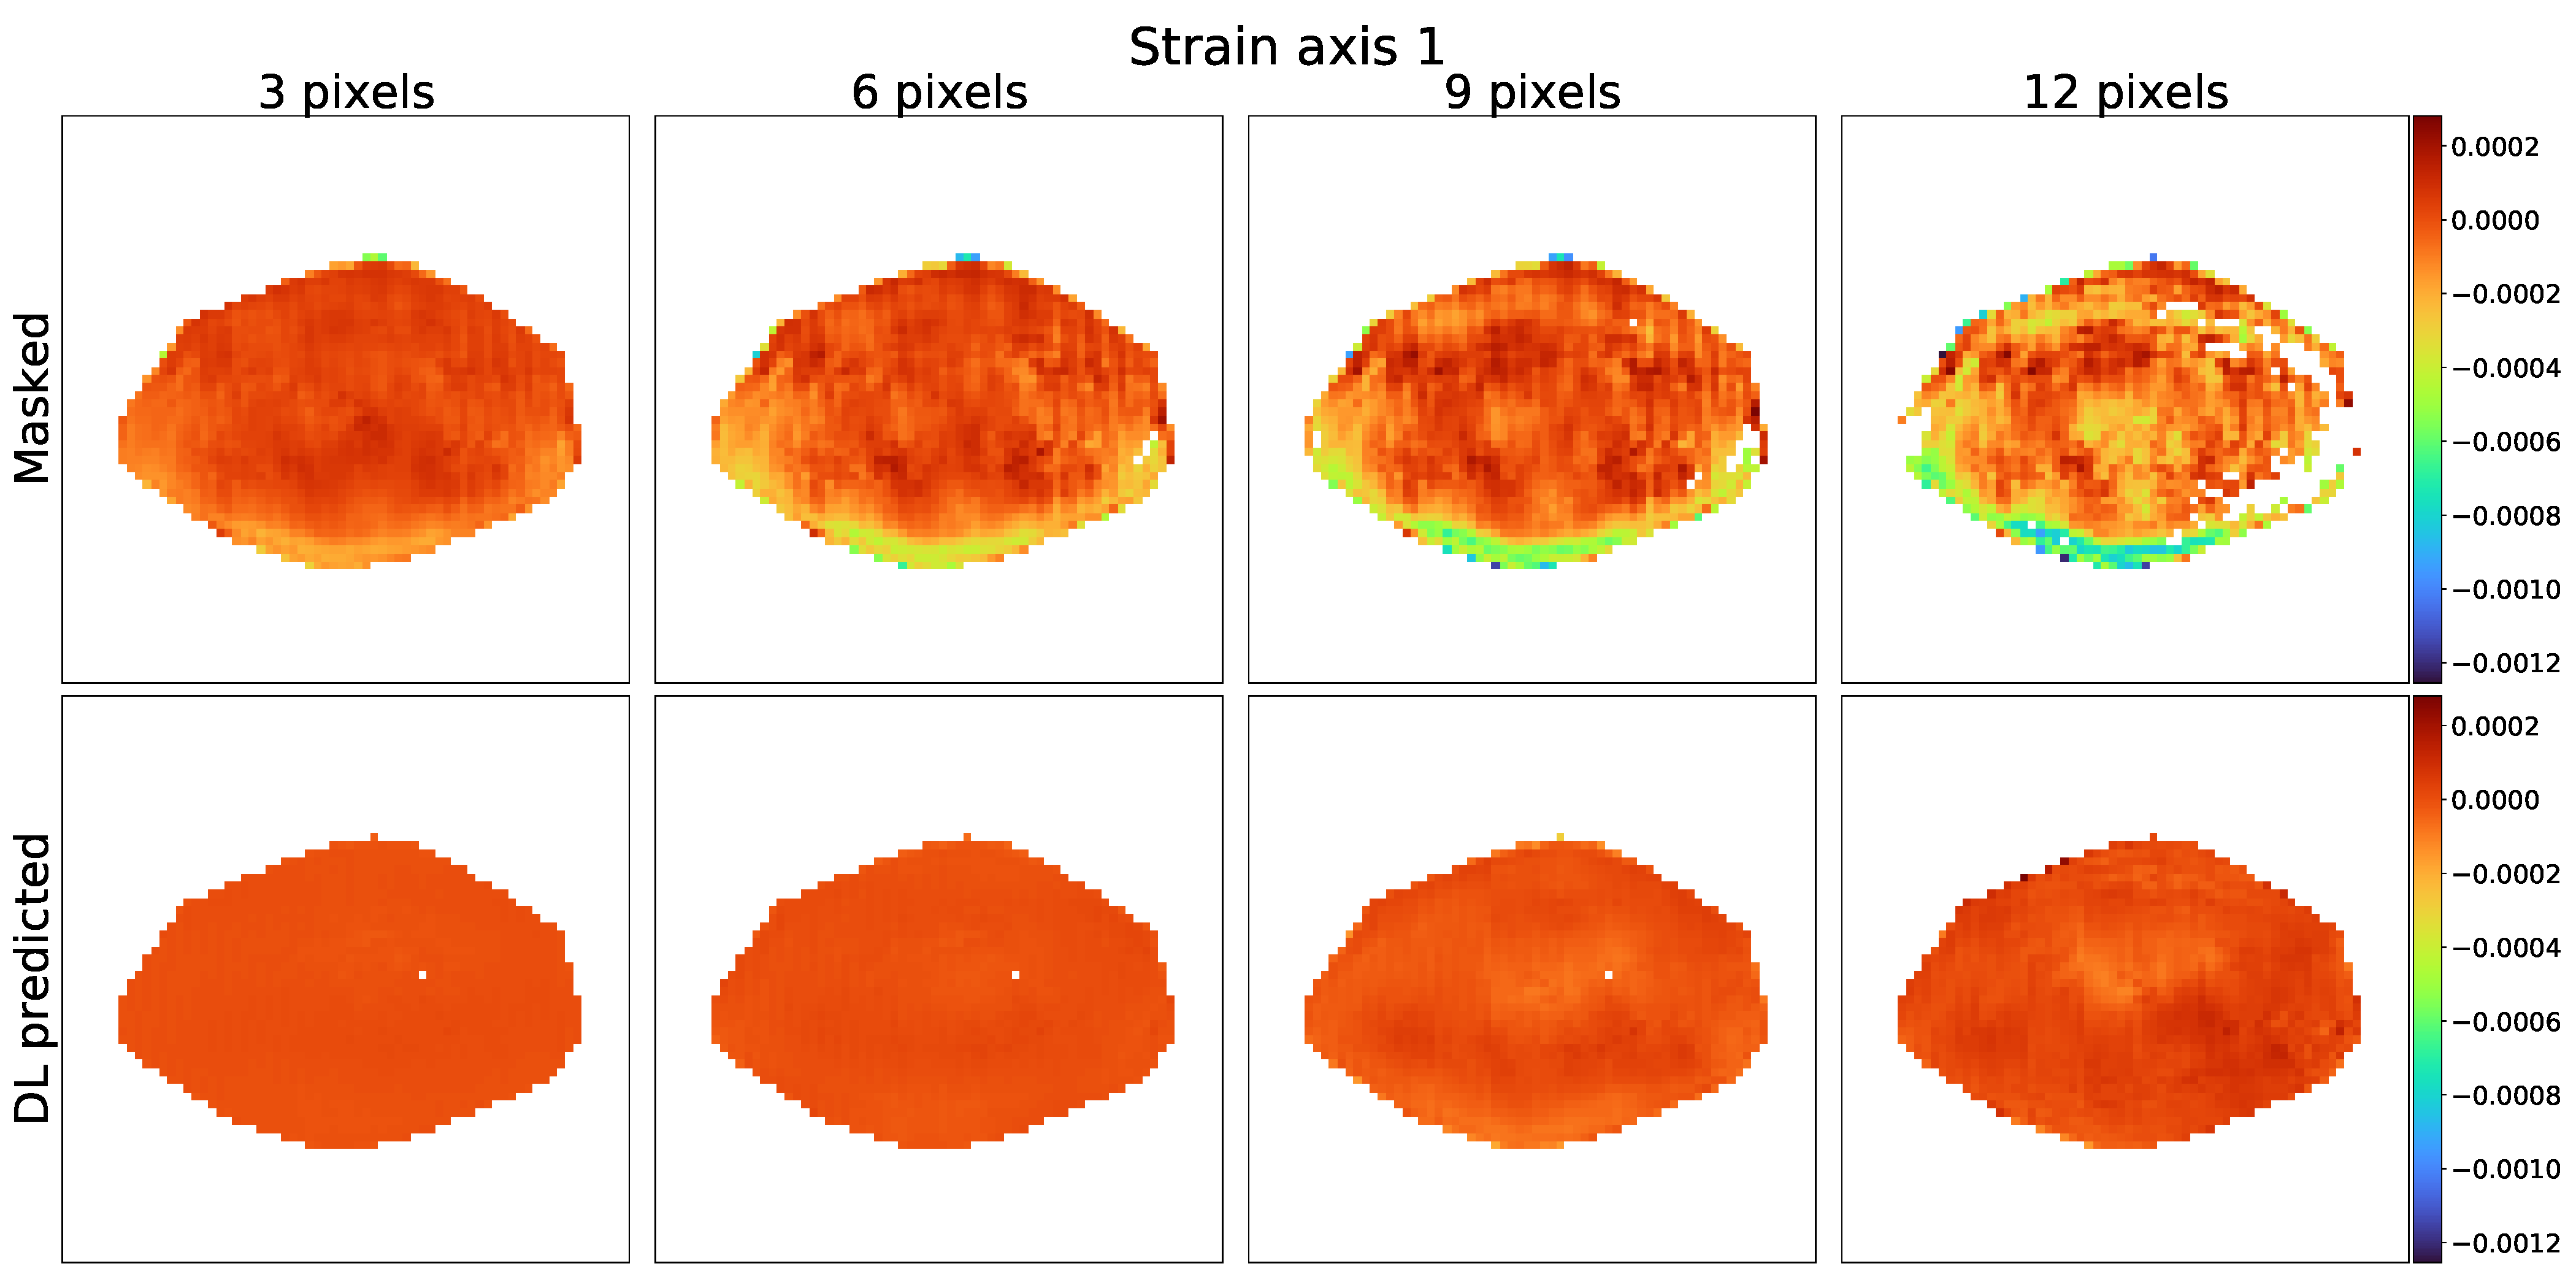
\includegraphics[width=\textwidth]{figures/Inpainting/strain_comparison_allGaps.pdf}
    \caption{Strain distribution in the central XZ slice of $\textbf{O}_{gap}$ for different gap sizes and 
    corresponding results for $\textbf{O}_{DL}$}
    \label{fig:Carnis_allgaps_strain}
\end{figure}

The deviation from the ground truth zero value of the retrieved strain for both $\textbf{O}_{gap}$ and $\textbf{O}_{DL}$
can be measured with the root mean squared error (RMSE) across all the different gap sizes. This calculation was already
proposed in the aforementioned work of Carnis and coauthors in which the results were plotted in Fig.4. We have reproduced
a similar figure adding the results of our DL model (Fig.\ref{fig:Carnis_std}). The trend of the strain RMSE 
resembles indeed the curve showed in \cite{carnis_towards_2019}, increasing significantly with the gap size 
while the DL equivalent curve lies below, dampening the error of approximately a factor 5. Moreover, the strain artifacts
induced by the gaps shift the average strain from the zero value as shown in Fig.\ref{fig:Carnis_avg} whereas our DL model 
maintains the average strain around zero.


\begin{figure}[H]
    \centering
    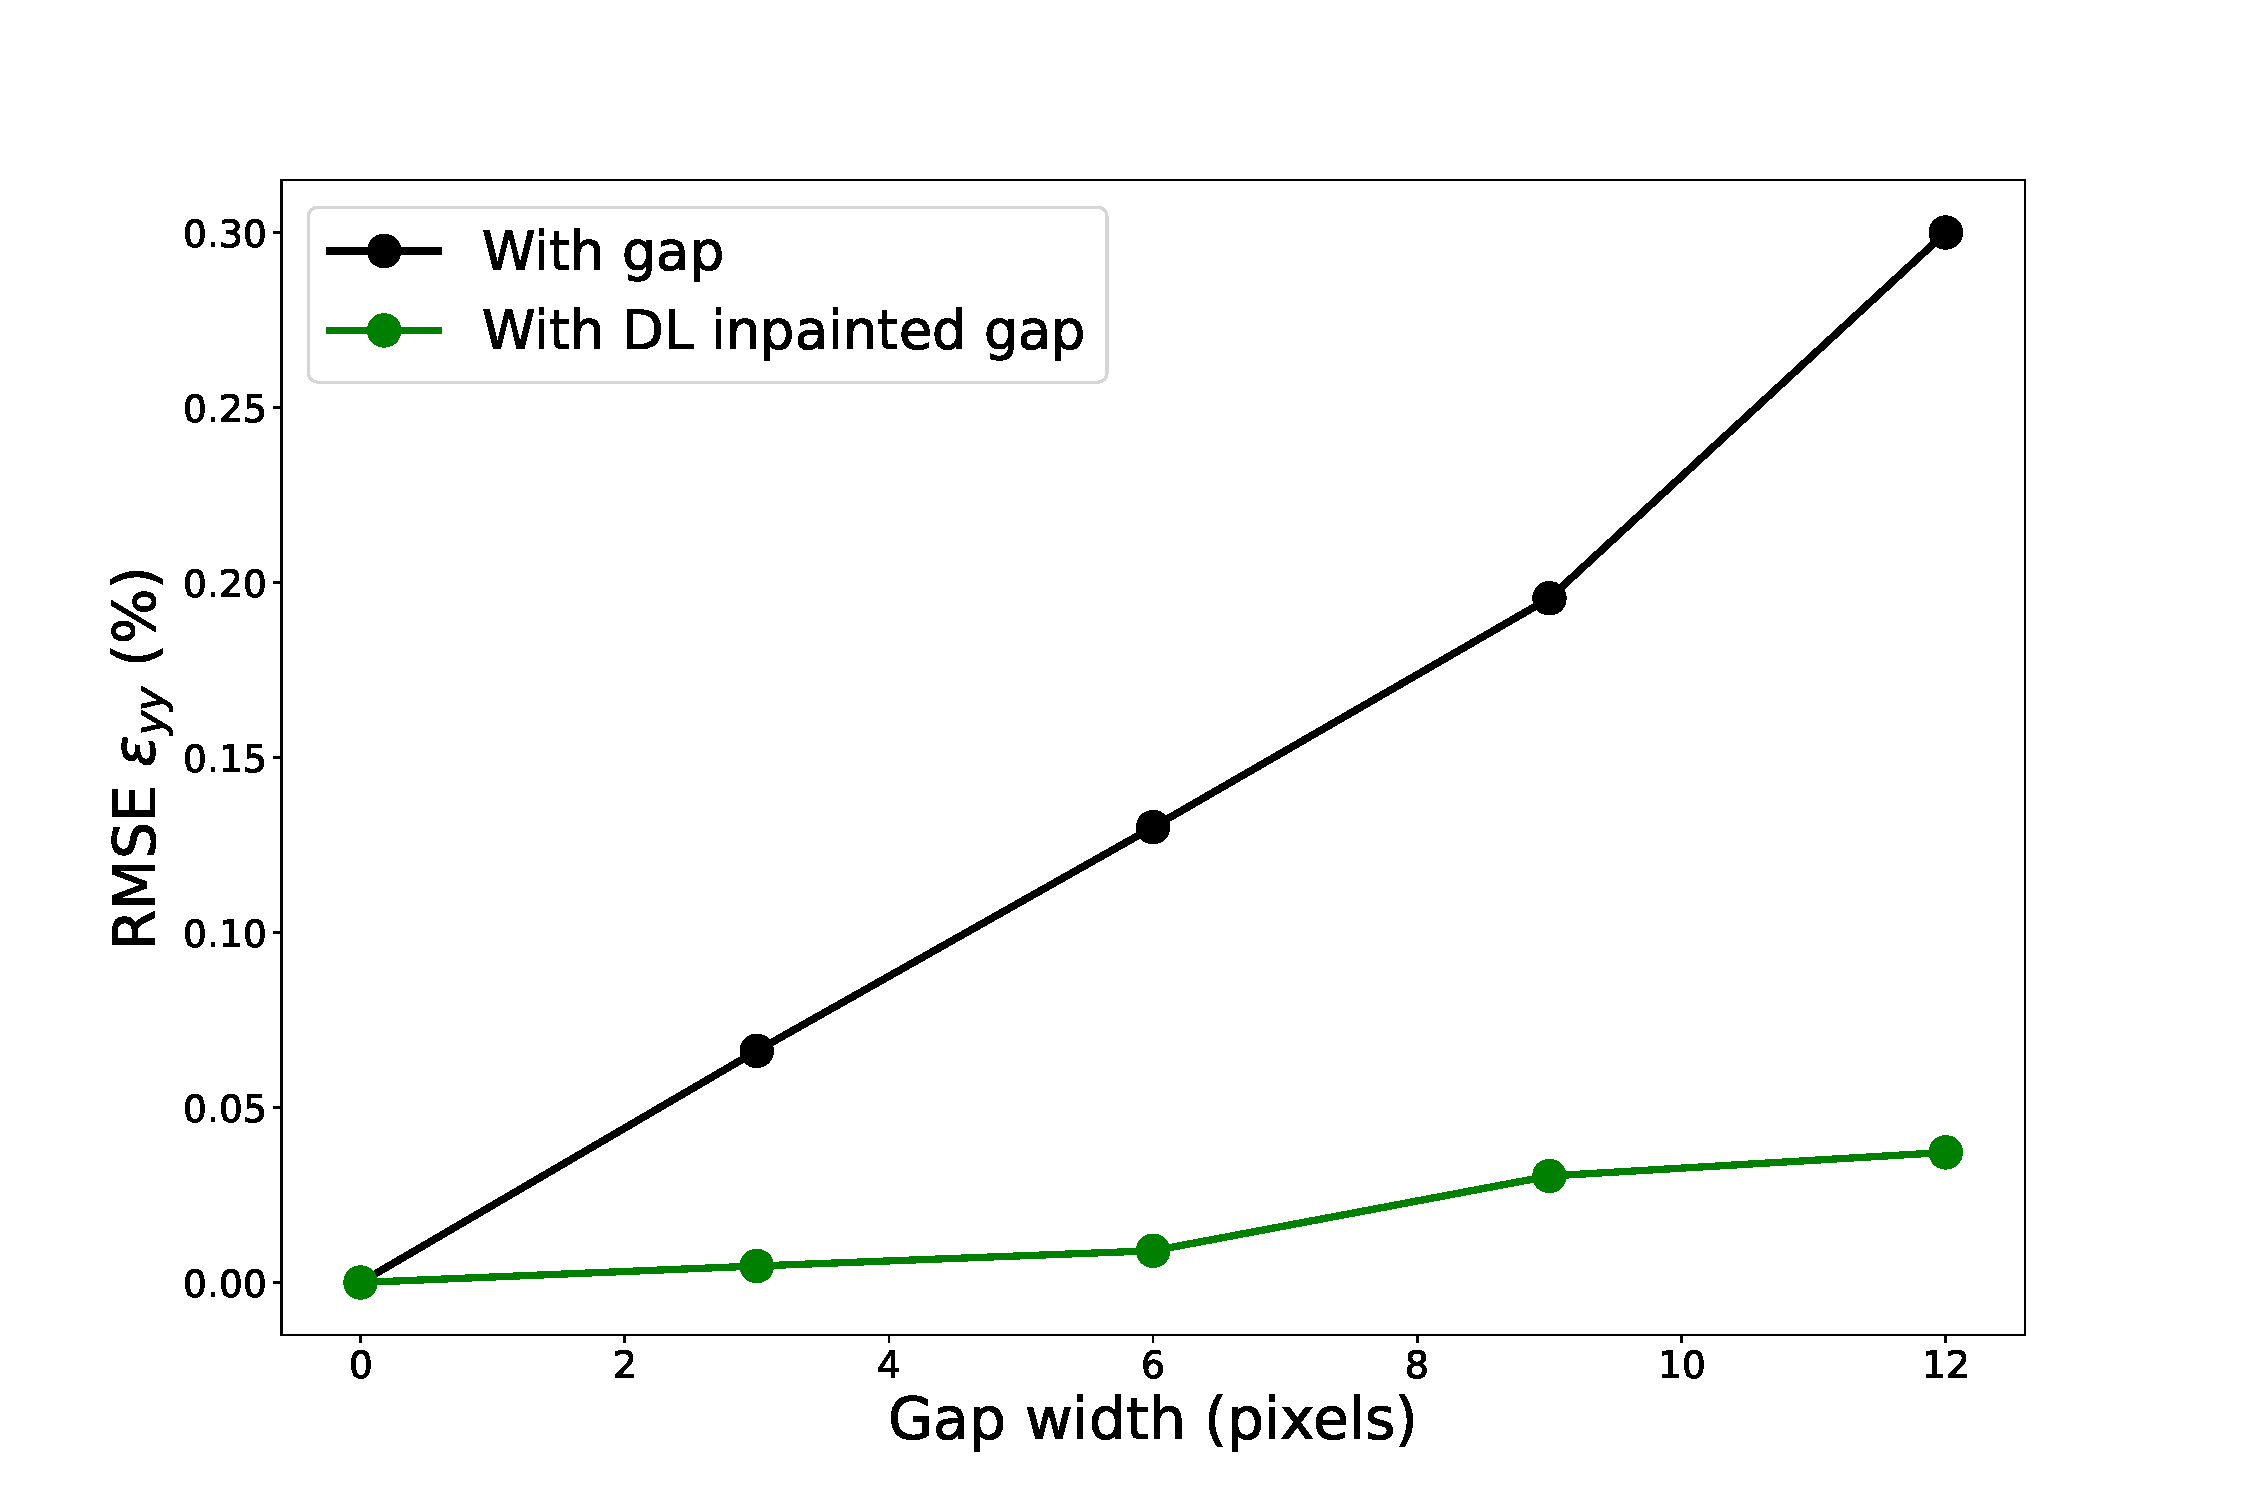
\includegraphics[width=\textwidth]{figures/Inpainting/std_strain_comparison.pdf}
    \caption{RMSE of the strain field versus gap size. For both cases of masked and DL inpainted diffraction
    patterns. For all gap sizes, the DL inpainted diffraction patterns yield a smaller error.
    }
    \label{fig:Carnis_std}
\end{figure}

\begin{figure}[H]
    \centering
    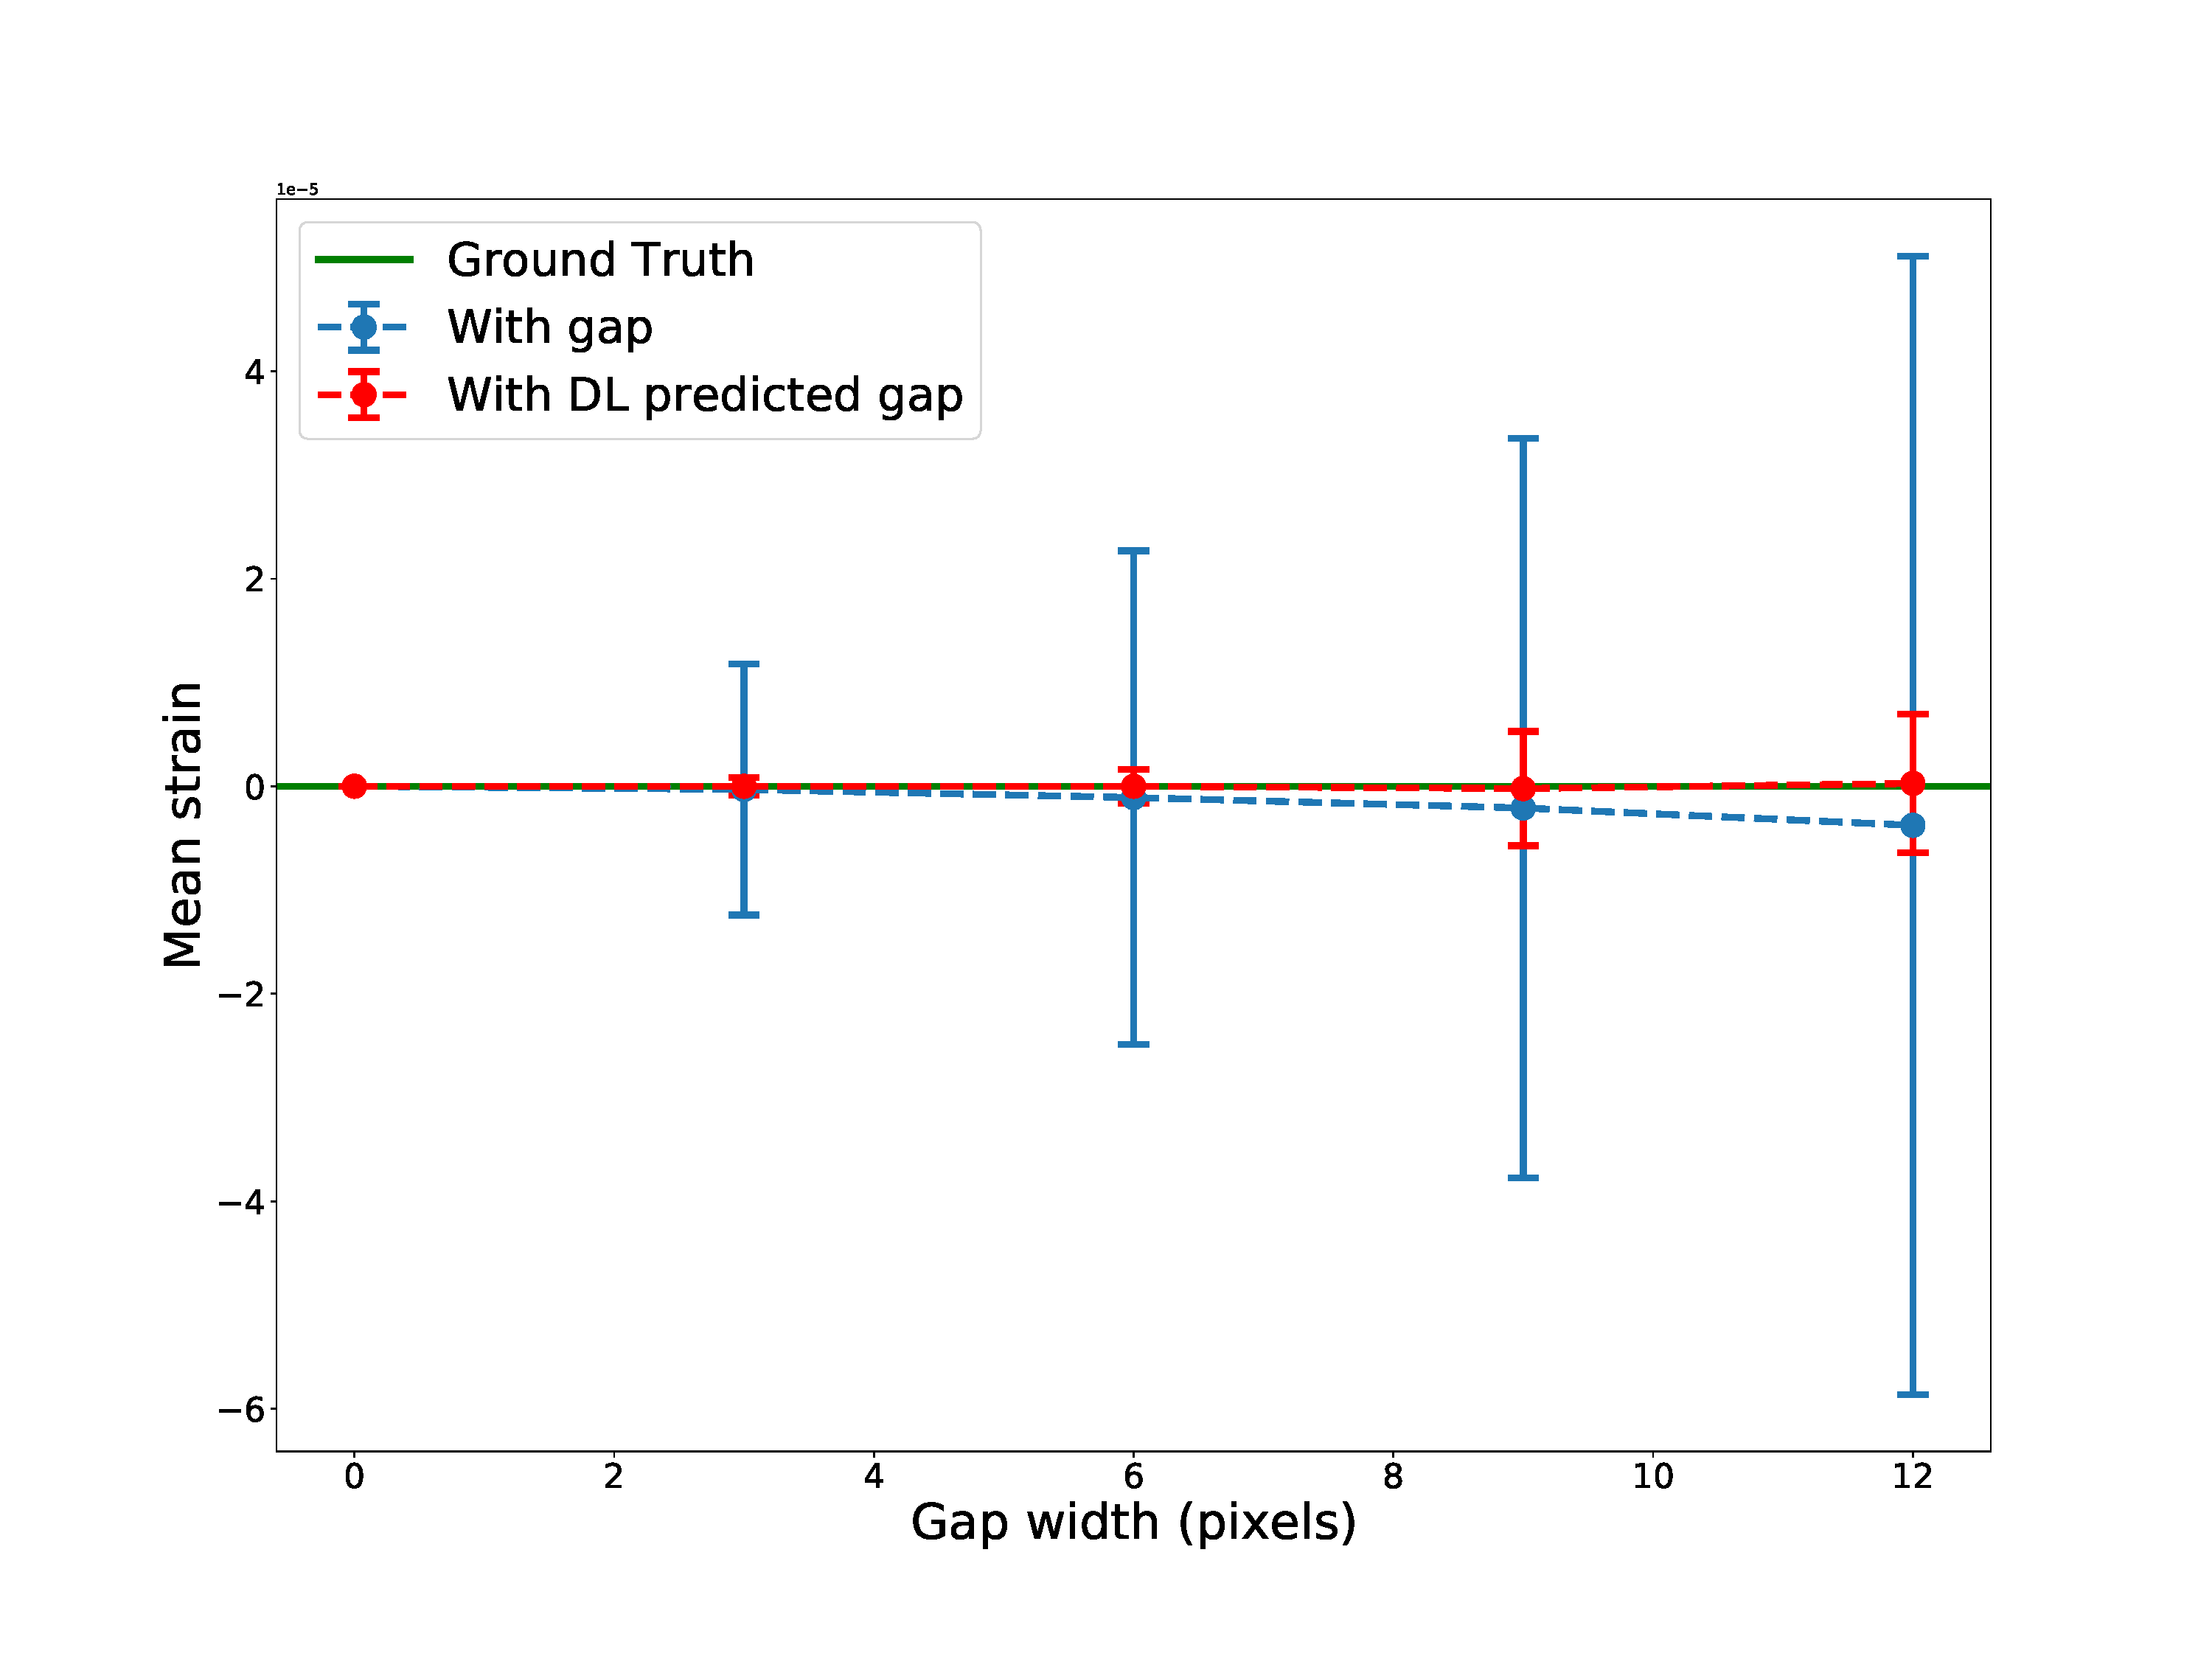
\includegraphics[width=\textwidth]{figures/Inpainting/avg_strain_comparison-1.pdf}
    \caption{RMSE of the strain field versus gap size.}
    \label{fig:Carnis_avg}
\end{figure}

\subsection{DL inpainting for high resolution BCDI}\label{sec:highres}
As anticipated in the introduction to the chapter, many of the cases in which a BCDI dataset is inevitably affected by 
a detector gap is the so-called ``high-resolution'' BCDI. The acquired data here extend for large $Q$ ranges in all
directions resulting in ROIs of several pixels. This can imply that parts of the diffracted signal crosses a region 
on the detector with a vertical or horizontal gap, thus needing for gap-inpainting. It is then convenient to use a
patching approach as treating the full volume would be computationally too expensive. Moreover, any binning or interpolation
to smaller sizes will induce information loss, as well not advised. \\
An example of high-resolution BCDI dataset of this type is the one we have used so far from the work of Carnis and coauthors. 
The original dataset is indeed a large ($256\times300\times300$ pixels) array that contains a cross-shaped, 6 pixel-wide 
gap. Here we show how the artifacts can change depending on the type of masking of the gaps is chosen during the phasing
and how our DL model can outperform these methods. 
A common approach, when using PyNX software, is to mask the gap such that those pixels don't contribute during the 
phasing and are left free to evolve (\textbf{a}). Moreover, one could mask only near the intensity streaks affected 
by the gap (\textbf{b}) or simply leave the gap with zeros and remove the contribution of the gap voxels during the whole phasing
(\textbf{c}). These strategies have been used during the phasing of the cited Pt diffraction pattern and the results 
in object space compared with what obtained from the DL inpainted pattern. The results, illustrated in Figs. \ref{fig:high_res_Icalc}
- \ref{fig:high_res_obj}, show that the amount of oscillatory artifacts progressively decreases as we go from method 
\textbf{a} to \textbf{c}, proving the DL inpainting to be the optimal method among them. 

\begin{figure}[H]
    \centering
    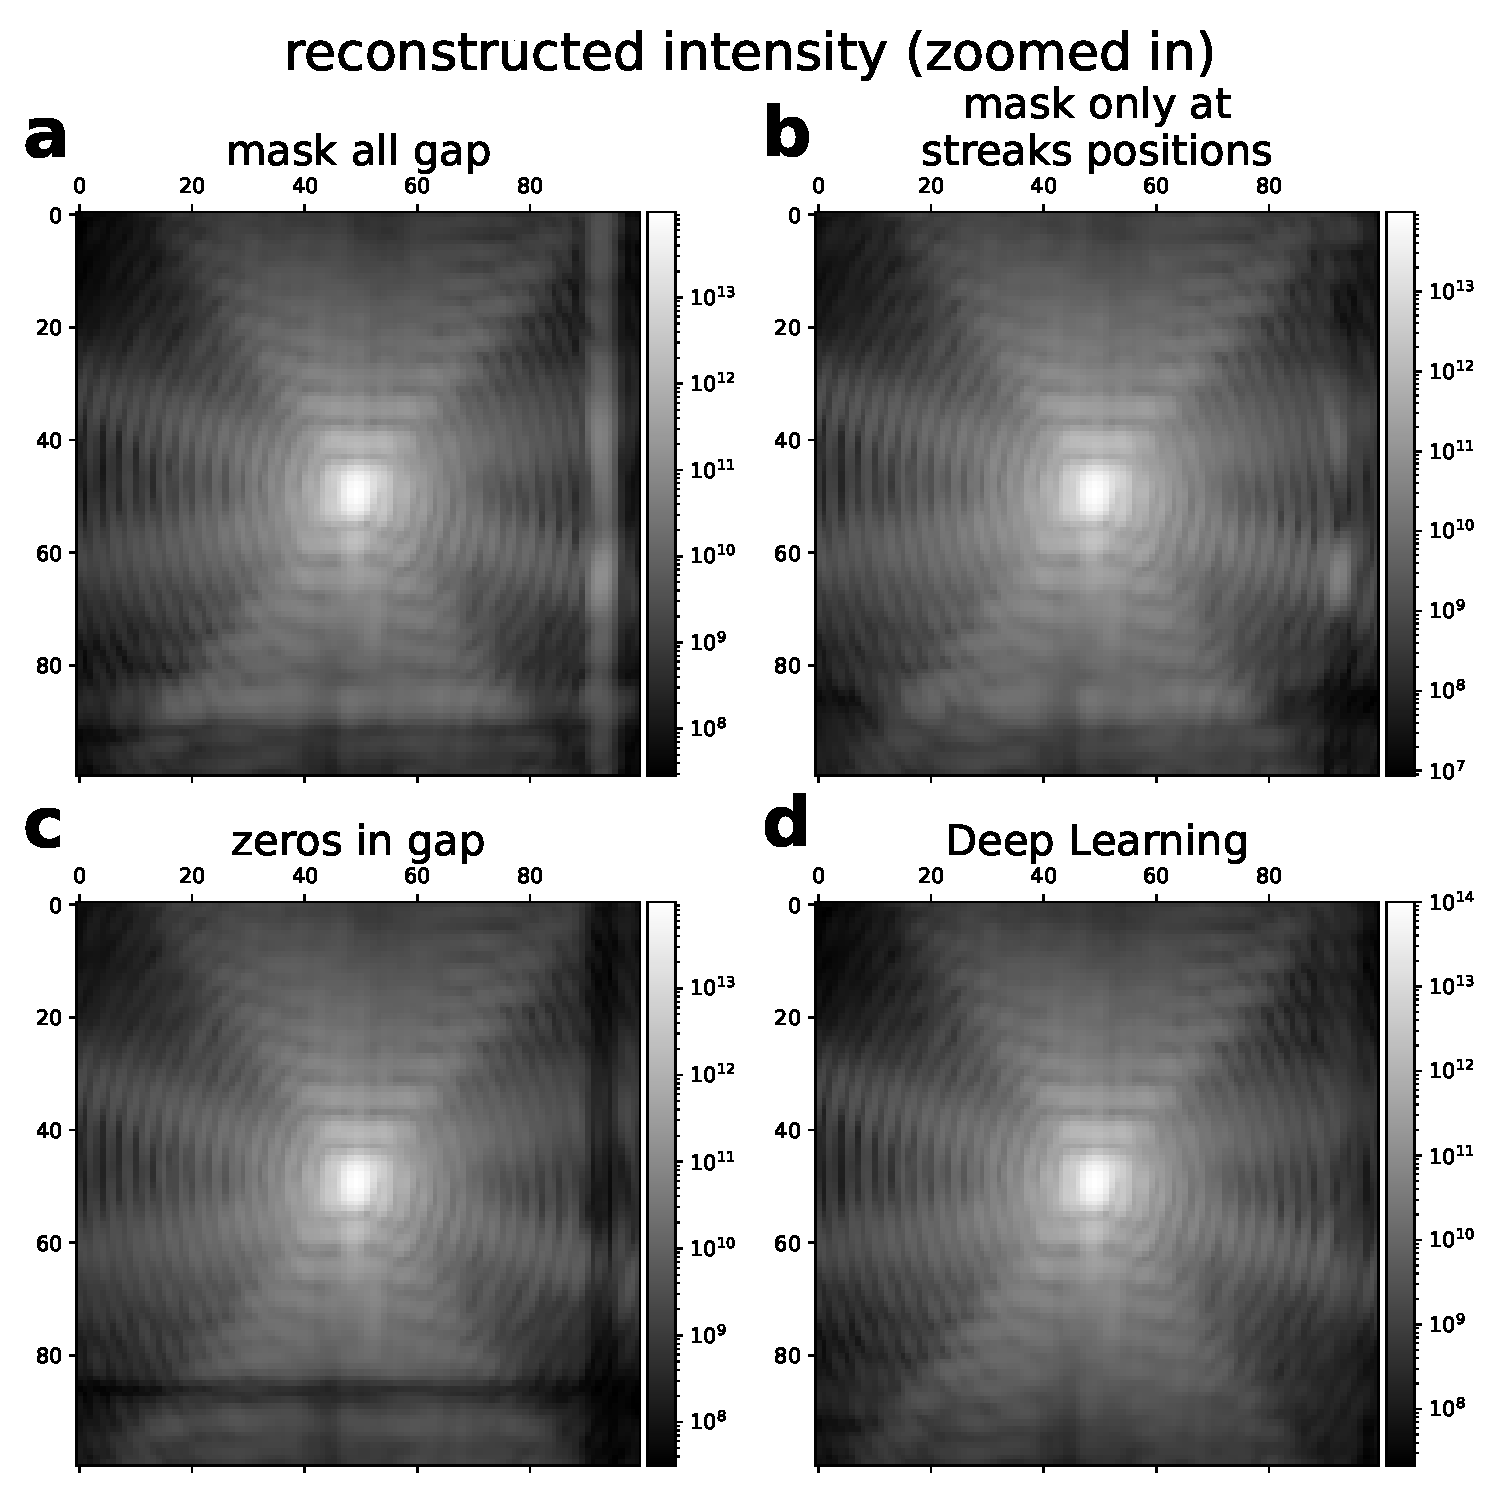
\includegraphics[width=\textwidth]{figures/Inpainting/reconstructed_intensity_zoom_jerome.pdf}
    \caption{Zoom on the projection along the rocking curve axis of the Pt THH BCDI pattern calculated from the reconstructed object 
    obtained with PyNX software using \textbf{a} a mask on the gaps, \textbf{b} a mask on the streaks only, leaving zeros 
    inside the gaps \textbf{c} and inpainting the gaps with our DL model. }
    \label{fig:high_res_Icalc}
\end{figure}

\begin{figure}[H]
    \centering
    \begin{subfigure}{0.47\textwidth} 
        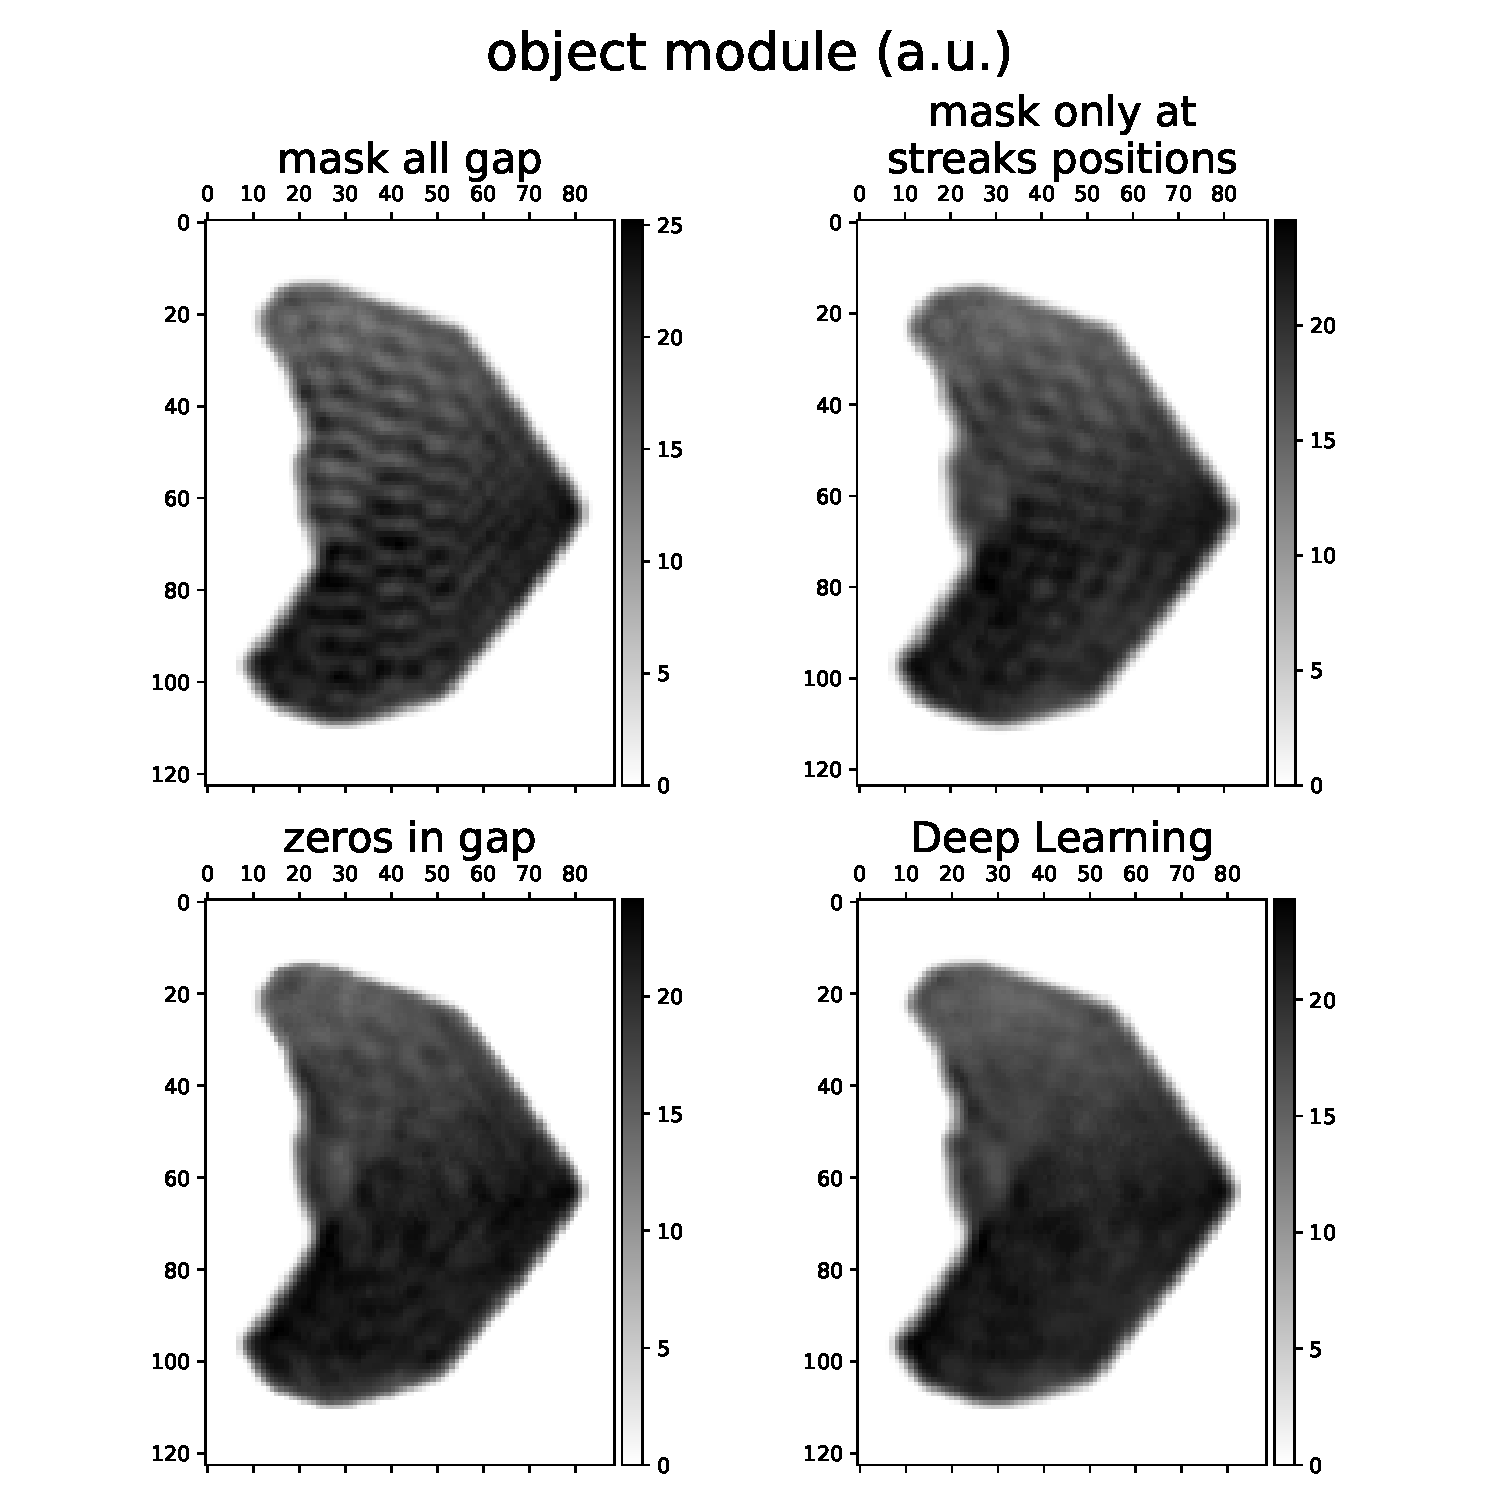
\includegraphics[width=\linewidth]{figures/Inpainting/object_module_jerome.pdf}
        \caption{\textbf{(a)}}
    \end{subfigure}
    \hfill
    \begin{subfigure}{0.47\textwidth}
        \centering
        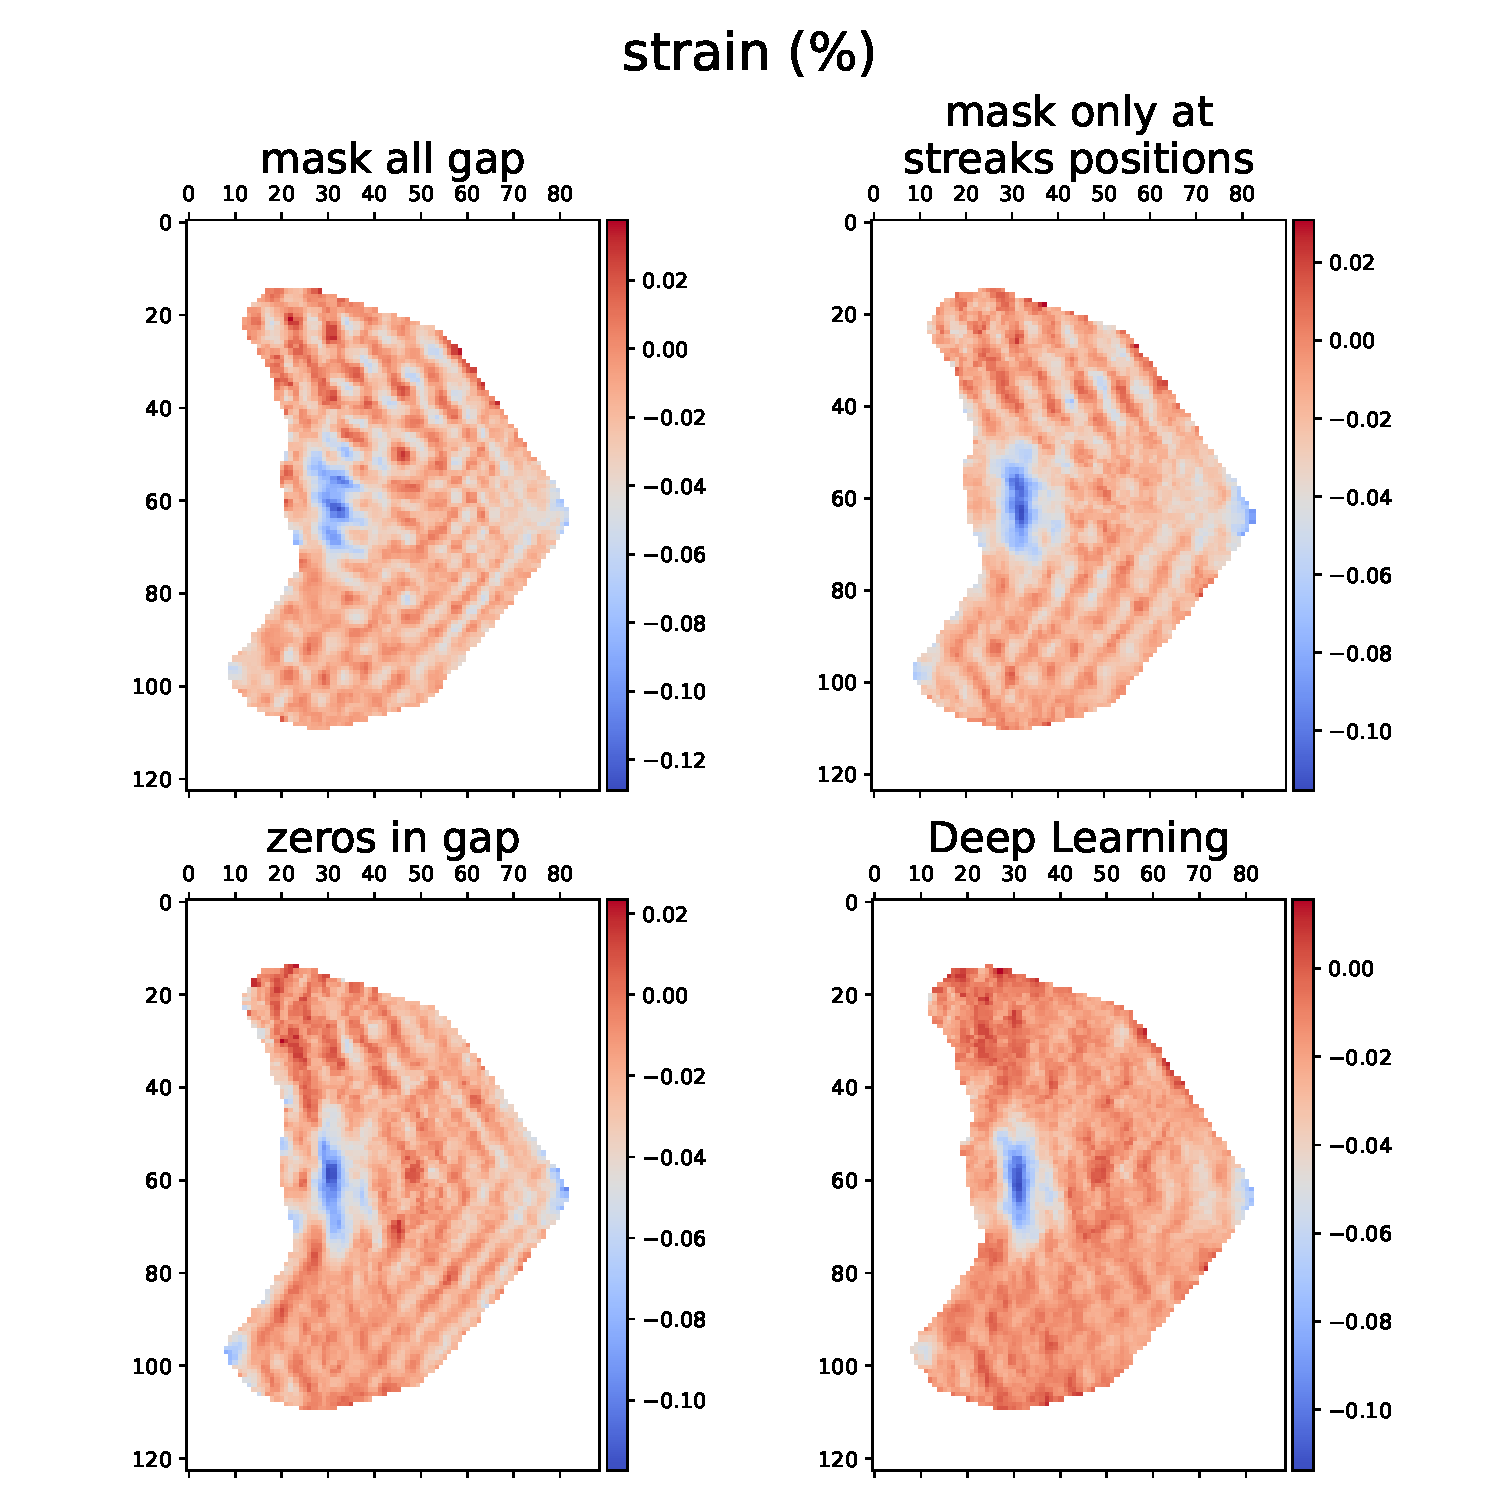
\includegraphics[width=\linewidth]{figures/Inpainting/object_strain_jerome.pdf}
        \caption{\textbf{(b)}}
    \end{subfigure}
    \caption{Modulus and strain of the object's reconstructions for each case mentioned above. The oscillatory artifacts
     are smallest for the object obtained after DL inpainting.}
    \label{fig:high_res_obj}
\end{figure}

\section{Fine-tuning}\label{sec:finetuning}
For those cases in which the DL model does not yield satisfactory results when inpainting a new experimental BCDI pattern 
we have thought about a fine-tuning of the model to improve the accuracy of the prediction. This fine-tuning is enabled by the 
patching approach as it consists of a secondary short training of the general model on a small dataset made of portions 
extracted from the new BCDI pattern to be inpainted.
In particular, after loading the gap affected BCDI pattern we have randomly cropped 6400 portions out of it, paying attention
not to include the gap region. We have then trained the model for the corresponding gap width for 5 epochs. Biasing the
model to the fit the features of that specific diffraction pattern (oversampling ratio, particle shape, noise level, fringes shape)
we could obtain better result on the real gap. An example is shown in Fig.\ref{sec:finetuning}. There, the general DL model
was not able to predict the fringes with the correct periodicity inside the gap. After the fine-tuning instead, the model 
properly recovers the fringes improving the accuracy. 
This fine-tuning technique wants to be a further example of the advantages of using a patching approach and its usage depends
on the user judgement on the quality of the general model inpainting. 

\begin{figure}[H]
    \centering
    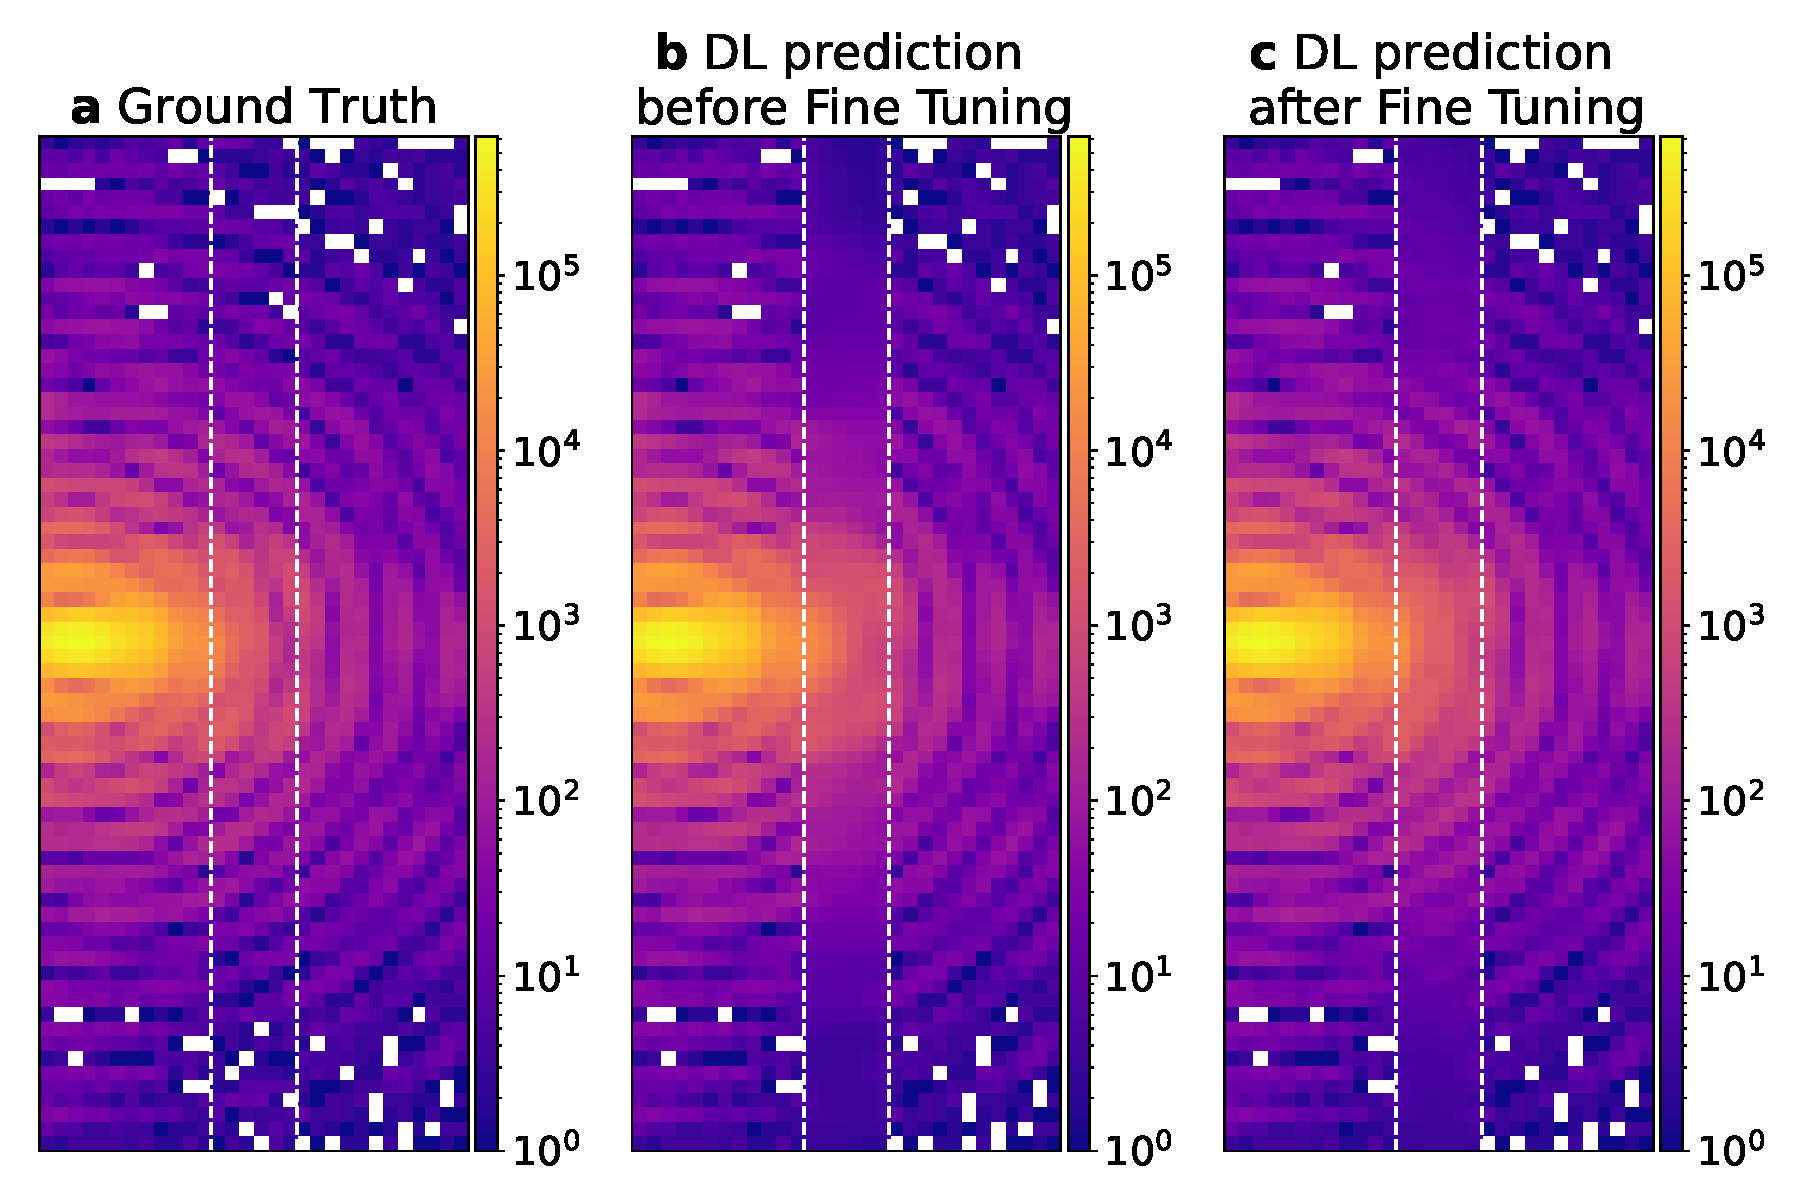
\includegraphics[width=\textwidth]{figures/Inpainting/FineTuning.pdf}
    \caption{Example of improved accuracy after fine-tuning of the DL model. The fringes are better recovered after 5 epochs
    of fine-tuning.}
    \label{fig:fine_tuning}
\end{figure}



% CHAPTER 5 - Deep Learning for Phase Retrieval
\chapter{Deep Learning for Phase Retrieval}
\label{chap:phase_retrieval}


We enter now the core topic of the thesis. Most of the efforts during this PhD have been dedicated to the study of the Phase Problem 
for Bragg Coherent Diffraction Imaging using DL based approaches. Here I will discuss the main steps of this
journey, starting off from the analysis of the most relevant works in literature and concluding with our final version
of a DL model for highly strained particles. The latter has become the subject of an article, currently in preparation, 
entitled ``\textit{Phase Retrieval of Highly Strained Bragg Coherent Diffraction Patterns with Supervised Convolutional 
Neural Network}''. The process that led to the final version of the model will be unraveled, and particular attention
 will be given to elucidating the key steps and the critical issues encountered along the way. 

\section{State of the art}\label{chp:phasing_stateart}
In this paragraph I will focus on the state of the art for what concerns the Phase Retrieval of BCDI diffraction patterns with
deep-learning, tensor-computation and automatic differentiation methods. Conventional phase retrieval iterative algorithms 
are discussed in the introduction chapter as well as other approaches. \\
Given the relatively new development of neural networks and more specifically even more recent for BCDI phase retrieval, I will try
to give a chronological broad overview over many of the main works in the literature pointing out strengths and weaknesses.
The first work pioneering the field is ``Real-time coherent diffraction inversion using deep generative networks'' published
by Cherukara \textit{et. al} in 2018 \cite{cherukara_real-time_2018}. The paper presents two CNNs for the phase retrieval of small ($32\times32$ pixels) 2D 
simulated BCDI patterns, one predicting the support and the other the phase. A U-Net like architecture with 
encoder-decoder was implemented, and the model was trained for just 10 epochs in a supervised fashion with a cross-entropy loss function (see Appendix).
The results showed an excellent agreement between prediction and ground truth also in presence of relatively strong phases. 
The potential of this new approach for phase retrieval becomes immediately clear when considering the drastic reduction of
computational time and resources needed for the model inference. Once the model is trained, the reconstruction can be obtained
within few milliseconds on a desktop machine. In 2020 Scheinker and Pokharel proposed another approach \cite{scheinker_adaptive_2020}
that employs a CNN model for 3D diffraction patterns. The fundamental difference is that the object's support was defined 
by its surface only, as it is assumed to be \textit{compact} and \textit{homogeneous} inside. Moreover, the surface was
parametrized by spherical harmonics and the DL model was trained to predict 28 of the first even coefficients of the spherical
harmonics. The model architecture was therefore essentially different since, while the encoder is just transposed to a 3D 
one, the decoder is replaced by a flattening and dense layer with 28 different classes as output. The model showed good performance
on both simulated and experimental data, marking the first DL-based approach capable of real 3D BCDI phase retrieval.
In the same year, Wu and coauthors, \cite{Wu2021}, opted for an architecture made of a single encoder and two identical decoders for the prediction of 
amplitude and phase of single crystals from the central slice of the BCDI pattern. They conducted the study on simulated 
data and tested it on one experimental case as well. What is evident from their work is the winning combination of DL prediction
and iterative refinement. The speed and generalization capabilities of the CNN allows for fast and good estimations of the 
object's support and phase. In addition, the precise and well established iterative methods can bring this initial guess to a 
more polished and accurate solution in fewer cycles than without DL prediction. This successful combined approach has been 
later adopted in other works, ours included. In 2021 two important works were published. First, Chan \textit{et al.} in 
\cite{chan_rapid_2021} extended the encoder/2-decoders architecture to the 3D case. In their work they first created a 
``physics-informed'' training set obtained building particles by clipping planes from a cubic FCC structure of atomic 
positions, relaxing them with LAMMPS software for molecular dynamics and computing the BCDI pattern around the (111) Bragg 
peak. The procedure is very similar to the one adopted by Lim \textit{et al.} in \cite{lim_convolutional_2021} and described
above in Section \ref{sec:dataset_creation3D}. Training the CNN on a restricted set of such created BCDI patterns biases 
the predictions towards physically meaningful particles. Moreover, it is interesting to notice that the training of the model 
was conducted in a sort of unsupervised fashion as the loss function calculates the differences between the target diffracted
intensity and the intensity obtained by the kinematic sum over the lattice sites of the predicted complex object.
Although the authors managed to successfully test their model on
an experimental BCDI pattern, the small size ($32\times32\times32$ pixels) of the images accepted by the CNN was not yet 
enough for proper experimental use. It's with the work of Wu \textit{et al.} \cite{wu_three-dimensional_2021} published 
in the same year, which lifted the size to 64 pixel-sided cubes, that the model can be tested on several experimental cases. 
Their CNN model maintained the encoder/2-decoders architecture for a simultaneous prediction of the object's amplitude and phase 
and explores for the first time the unsupervised training for refinement as well. The authors claimed that this approach is 
able to achieve better reconstruction quality with respect to current state-of-the-art iterative algorithms in use. 
The year after, Yao and coauthors published AutoPhaseNN \cite{yao_autophasenn_2022}, again an encoder/2-decoders architecture
that completely trained in an unsupervised manner. This approach is beneficial as it doesn't require datasets labeled with 
a ground truth, which means that experimental data can be directly used in the training set. Another advantage is that it 
overcomes the limitation of simulating an enough diverse population of samples, capable of constituting a comprehensive 
distribution of real cases. AutoPhaseNN was trained to predict an object the diffracted intensity of which matches the observed
one according to a normalized Mean Absolute Error metric. The model showed to work on simulated data as well as on experimental 
data and once more the winning method lies in the combination of DL prediction and iterative refinement. 
AutoPhaseNN has marked a milestone in the BCDI data analysis, attaining 10X to 100X phase retrieval speed up with reduced efforts 
for the model training. 
Although of different nature, it is worth mentioning the work of Zhuang and coauthors \cite{Zhuang2022PracticalPR} in which 
two CNNs are used in the ``deep image prior'' (DIP) framework. DIP \cite{Ulyanov_2020} typically implies the use of a CNN for 
an enhanced representation of an image, often to solve inverse problems like super-resolution, denoising and inpainting. 
However, it differs from classical deep learning as there is no training dataset but a fit of the target problem exploiting
the parameters of the convolutional layers and the efficient gradient descent provided by the automatic differentiation. 
In their work, Zhuang \textit{et al.} formulated the more general far-field phase retrieval problem as an optimization problem 
and considered the phase symmetries that affect this class of solutions (see Introduction chapter). Their work employs two 
DIPs, one for the modulus and one for the phase, and successfully manages to reconstruct simulated objects even in presence 
of strong phases. 
A last interesting contribution is the work of Yu and \textit{et al.} \cite{yu_ultrafast_2024}. In this paper the authors
proposed a DL model that computes complex convolutions, handling real and imaginary parts of the complex tensor in a single
passage through the convolutional block. Complex convolutional layers are claimed to be better at preserving the physical connection between real and imaginary parts  
inside the complex object. Moreover, the authors made use of \textit{skip connections} between encoder and decoder to 
enhance the training. This is a rather peculiar as this kind of residual links are typically used, in convolutional 
encoder-decoder networks, for tasks in which the input and output images are visually similar (i.e. segmentation, denoising, inpainting), 
thus, where it is more evident the information flow from the two blocks of the network. 
The model was used for the phase retrieval of experimental 2D diffraction patterns, for which an 
unsupervised refinement was used as well. \\
Before proceeding with our study, Table \ref{table:models} summarizes the key features of the works from the two 
leading BCDI research groups at Brookhaven and Argonne National Laboratories, highlighting similarities and 
differences to guide the development of our model.

\begin{table}[ht]
    \centering
    % \small
    \scriptsize
    % \renewcommand{\arraystretch}{0.9}
    \begin{tabular}{l|P{3.2cm}|P{2.2cm}|P{4.3cm}|P{3cm}}
    \textbf{} & \textbf{Architecture} & \textbf{Last Activation Layer} & \textbf{Loss Function} & \textbf{Refinement} \\
    \hline
    Cherukara - 2018 \cite{cherukara_real-time_2018} & Two different UNets & Sigmoids & Cross Entropy & - \\
    Wu - 2020 \cite{Wu2021} & Encoder / 2 Decoders & ReLU & MSE on mod and phase + PCC on magnitudes & Iterative \\
    Chan - 2021 \cite{chan_rapid_2021} & Encoder / 2 Decoders & ReLU & MAE on normalized magnitudes & Automatic Differentiation \\
    Wu - 2021 \cite{wu_three-dimensional_2021} & Encoder / 2 Decoders & LeakyReLU & MSE on mod and phase + PCC on magnitudes & Transfer learning + unsupervised training \\
    Yao - 2022 \cite{yao_autophasenn_2022} & Encoder / 2 Decoders & Sigmoid and Tanh & MAE on normalized magnitudes & Iterative (50 ER) \\
    Yu - 2024 \cite{yu_ultrafast_2024} & Complex encoder-decoder + skip connections & ReLU & MAE on real + MAE on imaginary & Transfer learning + unsupervised training
    \end{tabular}
    \caption{Comparison of deep learning-based phase retrieval approaches.}
    \label{table:models}
\end{table}
    
First, it is interesting to notice that the architecture's choice, from treating the object's modulus and phase separately 
with two different detached networks, moved over the years to a single ``standard'' U-Net that accounts for the complex 
nature of the data. Second, I noticed that the choice of the last activation layers, which are the ones producing the 
modulus and phase outputs, in their final value range, is not uniform throughout the articles. While ReLU and sigmoid
ensure real positive outputs, thus normally appropriate for real positive quantities like the modulus, LeakyReLU and Tanh  
allow for negative values as well, making them valid options for the phase array. Nevertheless, it seems that their impact is marginal 
since in some cases the model is able to predict correct moduli from LeakyReLUs and correct phases from ReLUs and sigmoids. 
Regarding this point, it is worth mentioning that a global offset of the phase that shifts the whole range to the real positive 
axis does not physically alter the solution. This would mean that a ReLU can still correctly yield a phase array, just shifted 
by a positive constant. The same holds for the sigmoid, as long as the phase span fits in the range of the activation function. 
\\
The most important component of the model is the loss function. Except the first work that employs a cross entropy loss, normally 
used for classification tasks, other works opt for MAE and MSE, of standard use for regression and PCC as well. Typically, 
when the loss is calculated between intensities the MAE and the PCC are used as they are more suitable for the high dynamic 
range of the diffraction patterns. MSE in fact, ``would overly de-emphasize errors in mid-intensity regions of the images''
\cite{chan_rapid_2021}.
Lastly, I have listed the different ways used to refine the DL predictions. Here we can notice that very soon GPU accelerated
gradient descent methods have been used in replacement of conventional iterative algorithms. The unsupervised training
allows to easily switch from inference to refinement using the same model in the same GPU optimized 
computing environment guaranteed by machine learning libraries like PyTorch and Tensorflow. 

\section{Reciprocal space phasing}\label{chp:phasing}

From the study of the literature I have started to delineate our approach, taking inspiration from these works but 
significantly changing the perspective. In particular, we have decided to predict the ``reciprocal space'' phase (RSP) that is 
lost during the measurement of the BCDI pattern rather than the complex object in real space.
The main, intuitive, reason behind this choice is that there is a visual 
similarity between the morphology of the diffraction pattern and its corresponding RSP. 
Furthermore, it is common that many samples studied with BCDI have facets that happen to be, to some degree, parallel with each other, 
thus interfering like a double-slit with the typical fringes of intensity that correspond to constructive interferences, 
interspersed with dark regions arising from destructive interferences. In these specific cases, the RSP shows a regular 
pattern in which there is always a $\pi$ shift between two crests of the fringes. (add something in the introduction)
Once retrieved the RSP one can then recompose the full complex diffracted wave-function and obtain the complex object via 
inverse Fourier transform.\\

\begin{figure}[H]
    \centering
    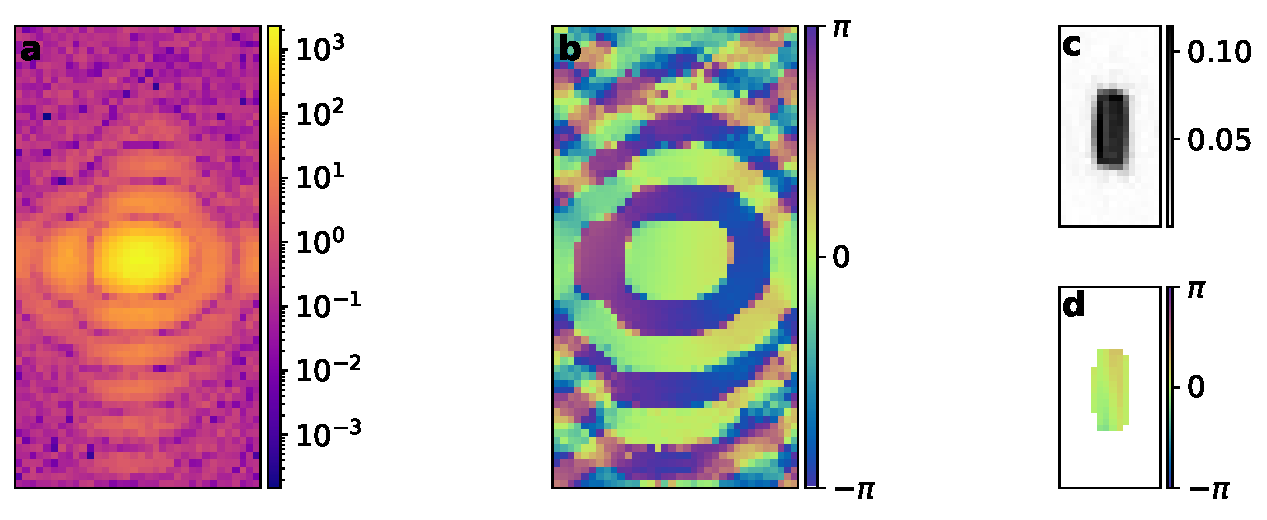
\includegraphics[width=.8\textwidth]{figures/Phasing/rec_space_phase.pdf}
    \caption{Central slice of a typical BCDI pattern (\textbf{a}) with the corresponding RSP (\textbf{b}) obtained after a 
    successful reconstruction of the object (modulus and phase in \textbf{c - d} respectively). It is clear the structural similarity between the diffracted intensity 
    in logarithmic scale and the RSP. Moreover, one can notice that in this case of low strain faceted particle, 
     the RSP varies regularly between 0 and $\pi$ (or $-\pi$) in correspondence of the intensity fringes. }
    \label{fig:rec_space_phase}
\end{figure}

Moreover, given this ``simple'' law of constructive-destructive interferences, we hypothesized the possibility to predict patches 
of this RSP given a portion of diffraction pattern and then, similarly to the inpainting case, stitch together them together
and obtain the full RSP. This entails a number of complications related to the so-called phase symmetries that I have encountered
during the development of the algorithms and that will be discussed in the next sections. \\
Ultimately, the goal of this DL model for phasing is to facilitate the reconstruction of highly strained particles. While 
other works in literature have mostly leveraged the gain in computing time, here the model aims at tackling those reconstructions for which 
conventional algorithms struggle to find convergence because of the high strain in the particle.   
However, in this case, the aforementioned RSP $\pi$-shifts in between two fringes is much more complicated since the 
strong and extended displacement fields inside the crystal alter the Bragg peak, merging and spreading the fringes 
into an irregularly distributed intensity pattern. I anticipate that this is what actually prevents the DL model 
from functioning on patches, for the high-strain case. It is however reported in this manuscript as it can help with the 
understanding of this complex problem and maybe serve in the future for further studies. 
% al punto che non si e' in grado di stabilire, a occhio, se l'informazione necessaria per costruire la mappa I-phi e' racchiusa in una porzione 
\section{Dataset creation} 

I have trained our model in a supervised manner, meaning, in this case, that the training was always conducted on simulated data 
only, as the RSP is never experimentally detectable. 
For this reason, I have simulated the training dataset following the same procedure described in Sections 
\ref{sec:dataset_creation2D} and \ref{sec:dataset_creation3D} for the 2D and 3D cases, respectively. However, in this
case, the dataset size was reduced to $64\times64\times64$ pixels, and no gap was applied. Additionally, I have used the 
calculated RSP as the ground truth label for training instead of the masked diffraction pattern.\\

I will anticipate here that for the high strain case I created a dedicated training set simulating the strain by applying 
an artificial ``strong'' phase to the particles. In order to have a diverse population of strain distributions I have 
simulated each object's phase using different functions and parameters, namely: with the sum of two Gaussian functions,
with the sum of two cosine functions and using a random Gaussian distribution. In each case, amplitudes, variances, 
frequencies, and correlation lengths were randomly chosen to ensure a phase variation within the particle ranging between 
$2\pi$ and $5\pi$. By doing this, I could obtain strongly distorted BCDI patterns, similar to experimental high-strain ones. 
In particular, the two Gaussian functions phase can closely emulate the effect of the substrate induced strain inside Winterbottom 
particles. 

\section{2D case low strain}\label{chp:2d_nostrain}
% MODEL 2D CASE NO STRAIN: SHOW THE MODEL PREDICTING THE PHASE AND USE A LOSS ON THE FOURIER TRANSFORM 
Alike the inpainting case, I have first conducted some preliminary studies in 2D, on noise-less low strain data. Here I will 
briefly show the model's architecture, the loss function and the results. 
\subsection{Model structure}
The architecture that I used has a U-Net like structure with an encoder and a decoder. 
The encoder is composed of six convolutional blocks through which the input diffracted intensity is progressively 
reduced from the 64 pixel-side squares to a 1D flattened vector. Each convolutional block is composed of a convolutional 
layer, a LeakyReLU activation function and a MaxPooling layer that halves the feature's map dimensions. (illustrate the 
parameters later). \\
At the end of the encoder the so-called bottleneck composed of a convolutional layer followed by a LeakyReLU activation 
processes the feature map before passing it to the decoder which, by means of transposed convolutions, LeakyReLU activations 
and UpSampling layers, brings back the feature map to the input's size. Skip connections between encoder and decoder blocks 
are employed as well. The output tensor is the result of a last single-channeled convolutional layer with no activation function. 
In this way we let the model predict unbounded tensors to account for the phase symmetries (see Intro). 

\subsection{Input preprocessing} 

Similarly to the inpainting case, the BCDI patterns have been transformed into logarithmic scale and normalized between 
0 and 1. Batches of 32 images at the time were used. 

\subsection{Loss function}
The choice of the loss function was firstly based on what was used in literature. 
A sum of the MSE computed on the objects' amplitudes and one on the phases has thus been used (Eq. \ref{eq:loss}). The ground truth 
objects were indeed available from the simulated data while the predicted objects have been first calculated with a 2D  
inverse Fourier transform from the diffracted amplitude and the predicted RSP (Eq. \ref{eq:ft_2D}). 
\begin{equation}
    \hat{o}(\mathbf{r})
    \;=\;
    \mathcal{F}^{-1}\!\bigl\{\sqrt{I(\mathbf{q})}\,e^{\,i\,\varphi_{\mathrm{pred}}(\mathbf{q})}\bigr\}(\mathbf{r})
    \quad,
    \label{eq:ft_2D}
\end{equation}

\begin{equation}
    \mathcal{L}
    \;=\;
    \frac{1}{N}\sum_{\mathbf{r}}
    \Bigl(\bigl|\hat{o}(\mathbf{r})\bigr|
        \;-\;\bigl|o(\mathbf{r})\bigr|\Bigr)^{2}
    \;+\;
    \frac{1}{N}\sum_{\mathbf{r}}
    \Bigl(\phi(\mathbf{r})
        \;-\;\phi_{\mathrm{gt}}(\mathbf{r})\Bigr)^{2}
    \quad,
    \label{eq:loss}
\end{equation}

\subsection{Results}
The training of the model was conducted on 8500 simulated BCDI patterns over 30 epochs with a learning rate of 0.0003
and monitored both training and validation loss. Here, Fig.\ref{fig:loss_2mse_nosymm} shows the model's loss during the 
30 epoch long training. However, despite the good decaying trend, typical of proper training, the model does not 
perform optimally when tested on new data. 

\begin{figure}[H]
    \centering
    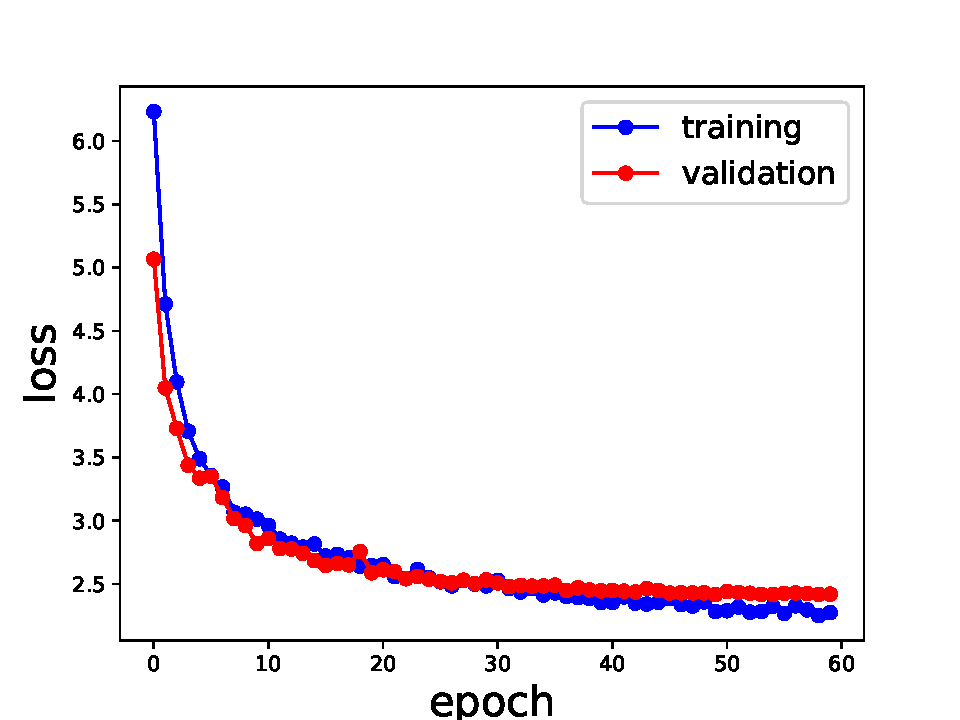
\includegraphics[width=.8\textwidth]{figures/Phasing/loss_low_strain_noiseless_doubleMSE_nosymm.pdf}
    \caption{Training and validation loss over 30 epochs. The curve suggests a proper learning with no overfitting as 
    both losses are decreasing reaching a plateau and the validation loss follows the same trend of the training loss.}
    \label{fig:loss_2mse_nosymm}
\end{figure}

Fig.\ref{fig:RSP_lowStrain_doubleMSE} illustrates the results of the predicted RSP of some test simulated BCDI patterns. 
Note that the displayed predicted RSP has been wrapped between 0 and 2$\pi$ for better comparison with the ground truth 
but the raw output of the model is in fact an ``unwrapped'' array. This is expected since no activation layer was applied 
to the last convolutional layer, meaning that the last operation is the multiplication of the last feature map with the 
real values inside the convolutional kernel, hence linear. \\
When comparing the reconstructed objects obtained from the predicted RSP with the ground truth ones (Fig. \ref{fig:obj_lowStrain_doubleMSE})
one can draw some interesting conclusions about the model's learning performances. 
First it can be observed that the model learns the approximate shape and size of the particle, it produces indeed images 
that resemble reasonable particles, sometimes similar to the ground truth ones. The amplitude is concentrated inside 
the support with little noise outside and the phase is overall correct around zero. However, when looking more carefully, 
it is clear that the shape is not quite correct, especially for highly non-centrosymmetric objects. For instance, if we 
consider the object in Fig. \ref{fig:obj_lowStrain_doubleMSE} \textbf{c}, we see that the predicted shape seems to be 
deriving from the incorrect superposition of the correct shape and its twin, as well correct. More in general it seems 
that the model tends to predict centrosymmetric objects. According to Sicairos \textit{et al.} \cite{guizar-sicairos_understanding_2012}, 
if we name $\varphi(\vec{q})$ the correct RSP, this phenomenon is originated by a predicted RSP phase $\phi$ composed 
of $\varphi(\vec{q})$ in some regions of the $q$-space and $-\varphi(\vec{q})$ elsewhere. In other words, the model is not 
fully able to break the sign symmetry. This subject was recently studied by Zhang and coauthors in \cite{zhang_what_2024}. 
In their study, the authors show that if not broken in the dataset, meaning that during the 
training the model is exposed to both cases ($\varphi(\vec{q})$ and $-\varphi(\vec{q})$) indistinctly, the model is deceived 
to a mix of the two, since the sign information cannot be recovered from the input intensity. The authors conclude that 
in order prevent this detrimental effect, one should break the symmetry in the dataset to bias the model towards one 
preferred sign. 

\begin{figure}[H]
    \centering
    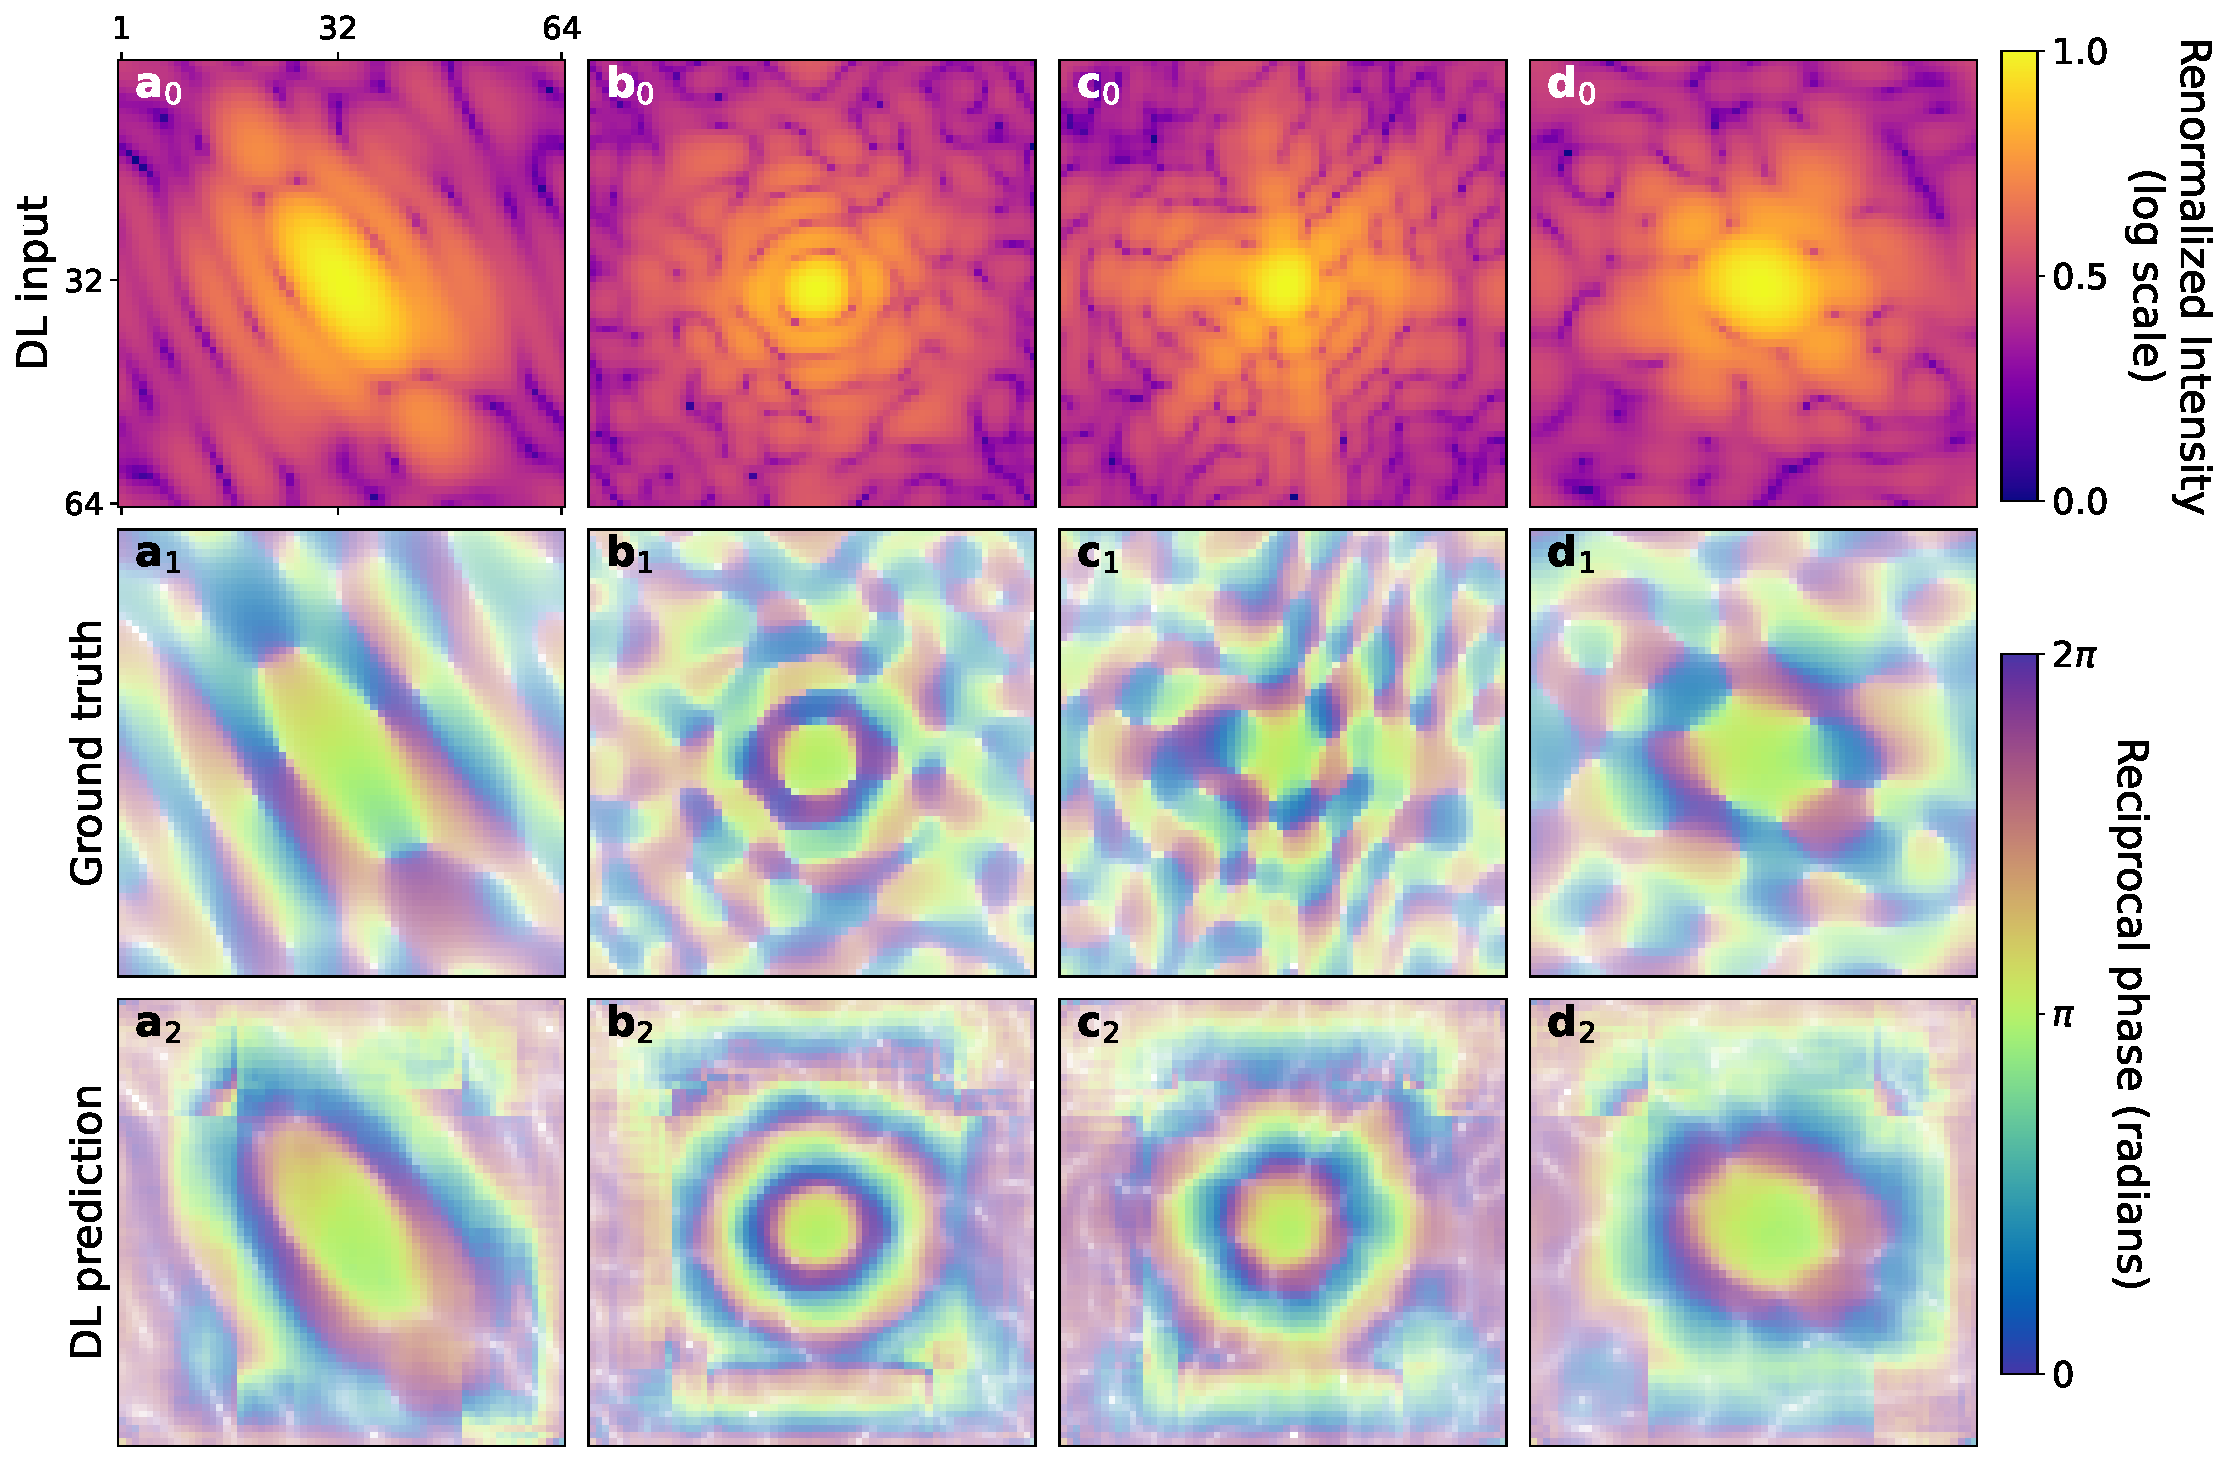
\includegraphics[width=.8\textwidth]{figures/Phasing/RSP_low_strain_doubleMSE.pdf}
    \caption{\textbf{Model testing on new 2D data using MSE loss function}. First row shows four simulated BCDI patterns, second row the ground truth RSP 
    corresponding to the pattern and last row the DL prediction }
    \label{fig:RSP_lowStrain_doubleMSE}
\end{figure}
\begin{figure}[H]
    \centering
    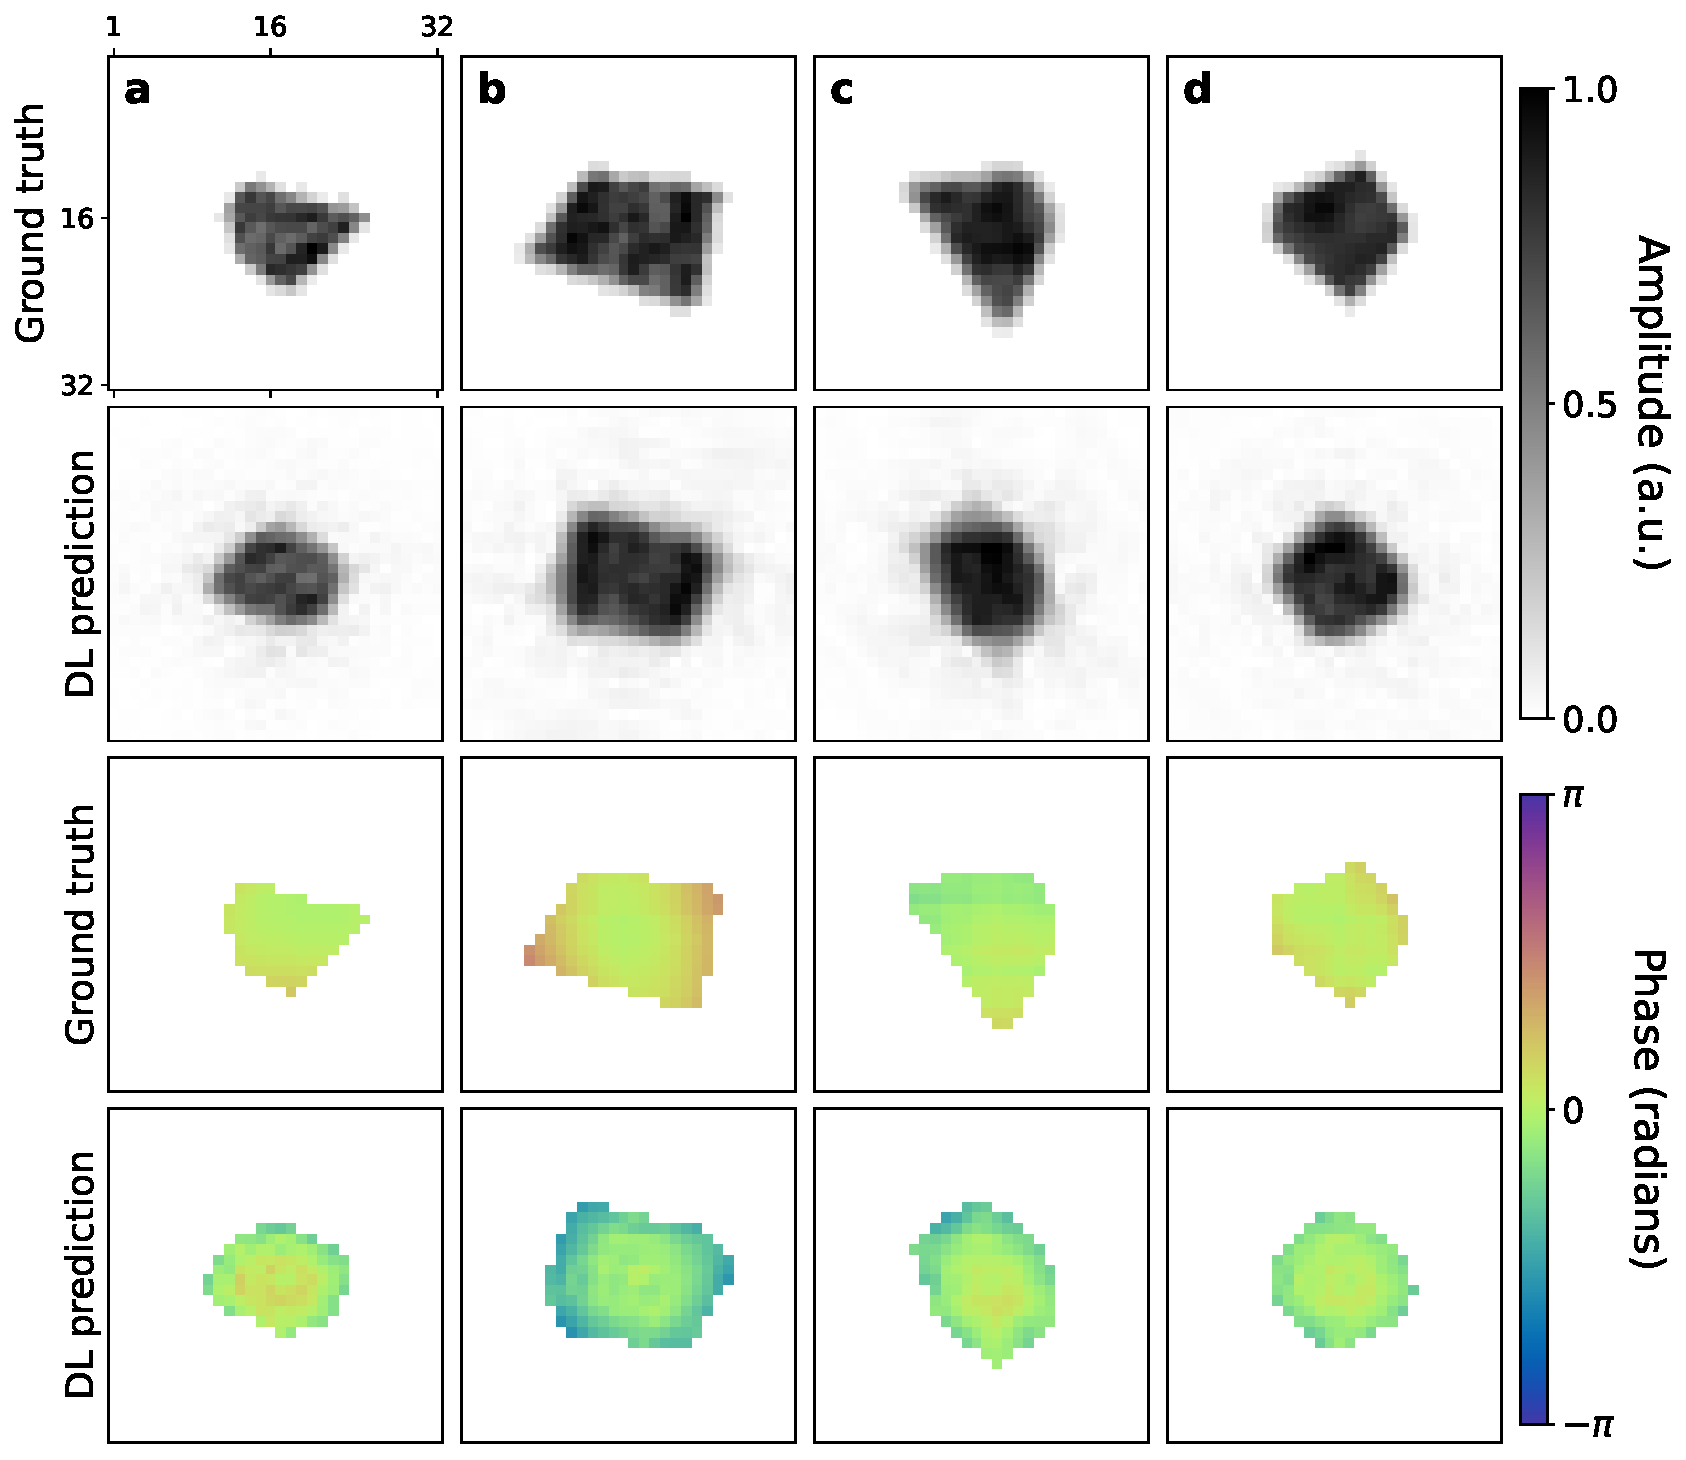
\includegraphics[width=.8\textwidth]{figures/Phasing/obj_low_strain_doubleMSE.pdf}
    \caption{\textbf{Corresponding reconstructed objects}. Ground truth and predicted objects' amplitudes (first two rows 
    respectively) and ground truth and predicted objects' phases (first two rows respectively)}
    \label{fig:obj_lowStrain_doubleMSE}
\end{figure}


The procedure presented in the article for the removal of the phase symmetries consists in: (i) the centering of all the 
objects in real space (phase ramp removal), (ii) the shift of the RSP such that the zero value in the same array position 
across the dataset (phase offset removal), and lastly, (iii) they flip the sign of the RSP when its value in corresponding 
to a fixed position across the dataset is negative. In our case the phase ramp symmetry was already broken by simulating 
particles with the center of mass in the center of the array. In this way the model is already biased towards the prediction 
of RSPs that yield centered objects. For the offset and the sign, the method proposed by Zhang \textit{et al.} has been 
implemented in the model and the results are shown in Fig. \ref{fig:RSP_lowStrain_doubleMSE_JuSun} for the RSP and 
Fig. \ref{fig:obj_lowStrain_doubleMSE_JuSun} for the reconstructed objects. 

\begin{figure}[H]
    \centering
    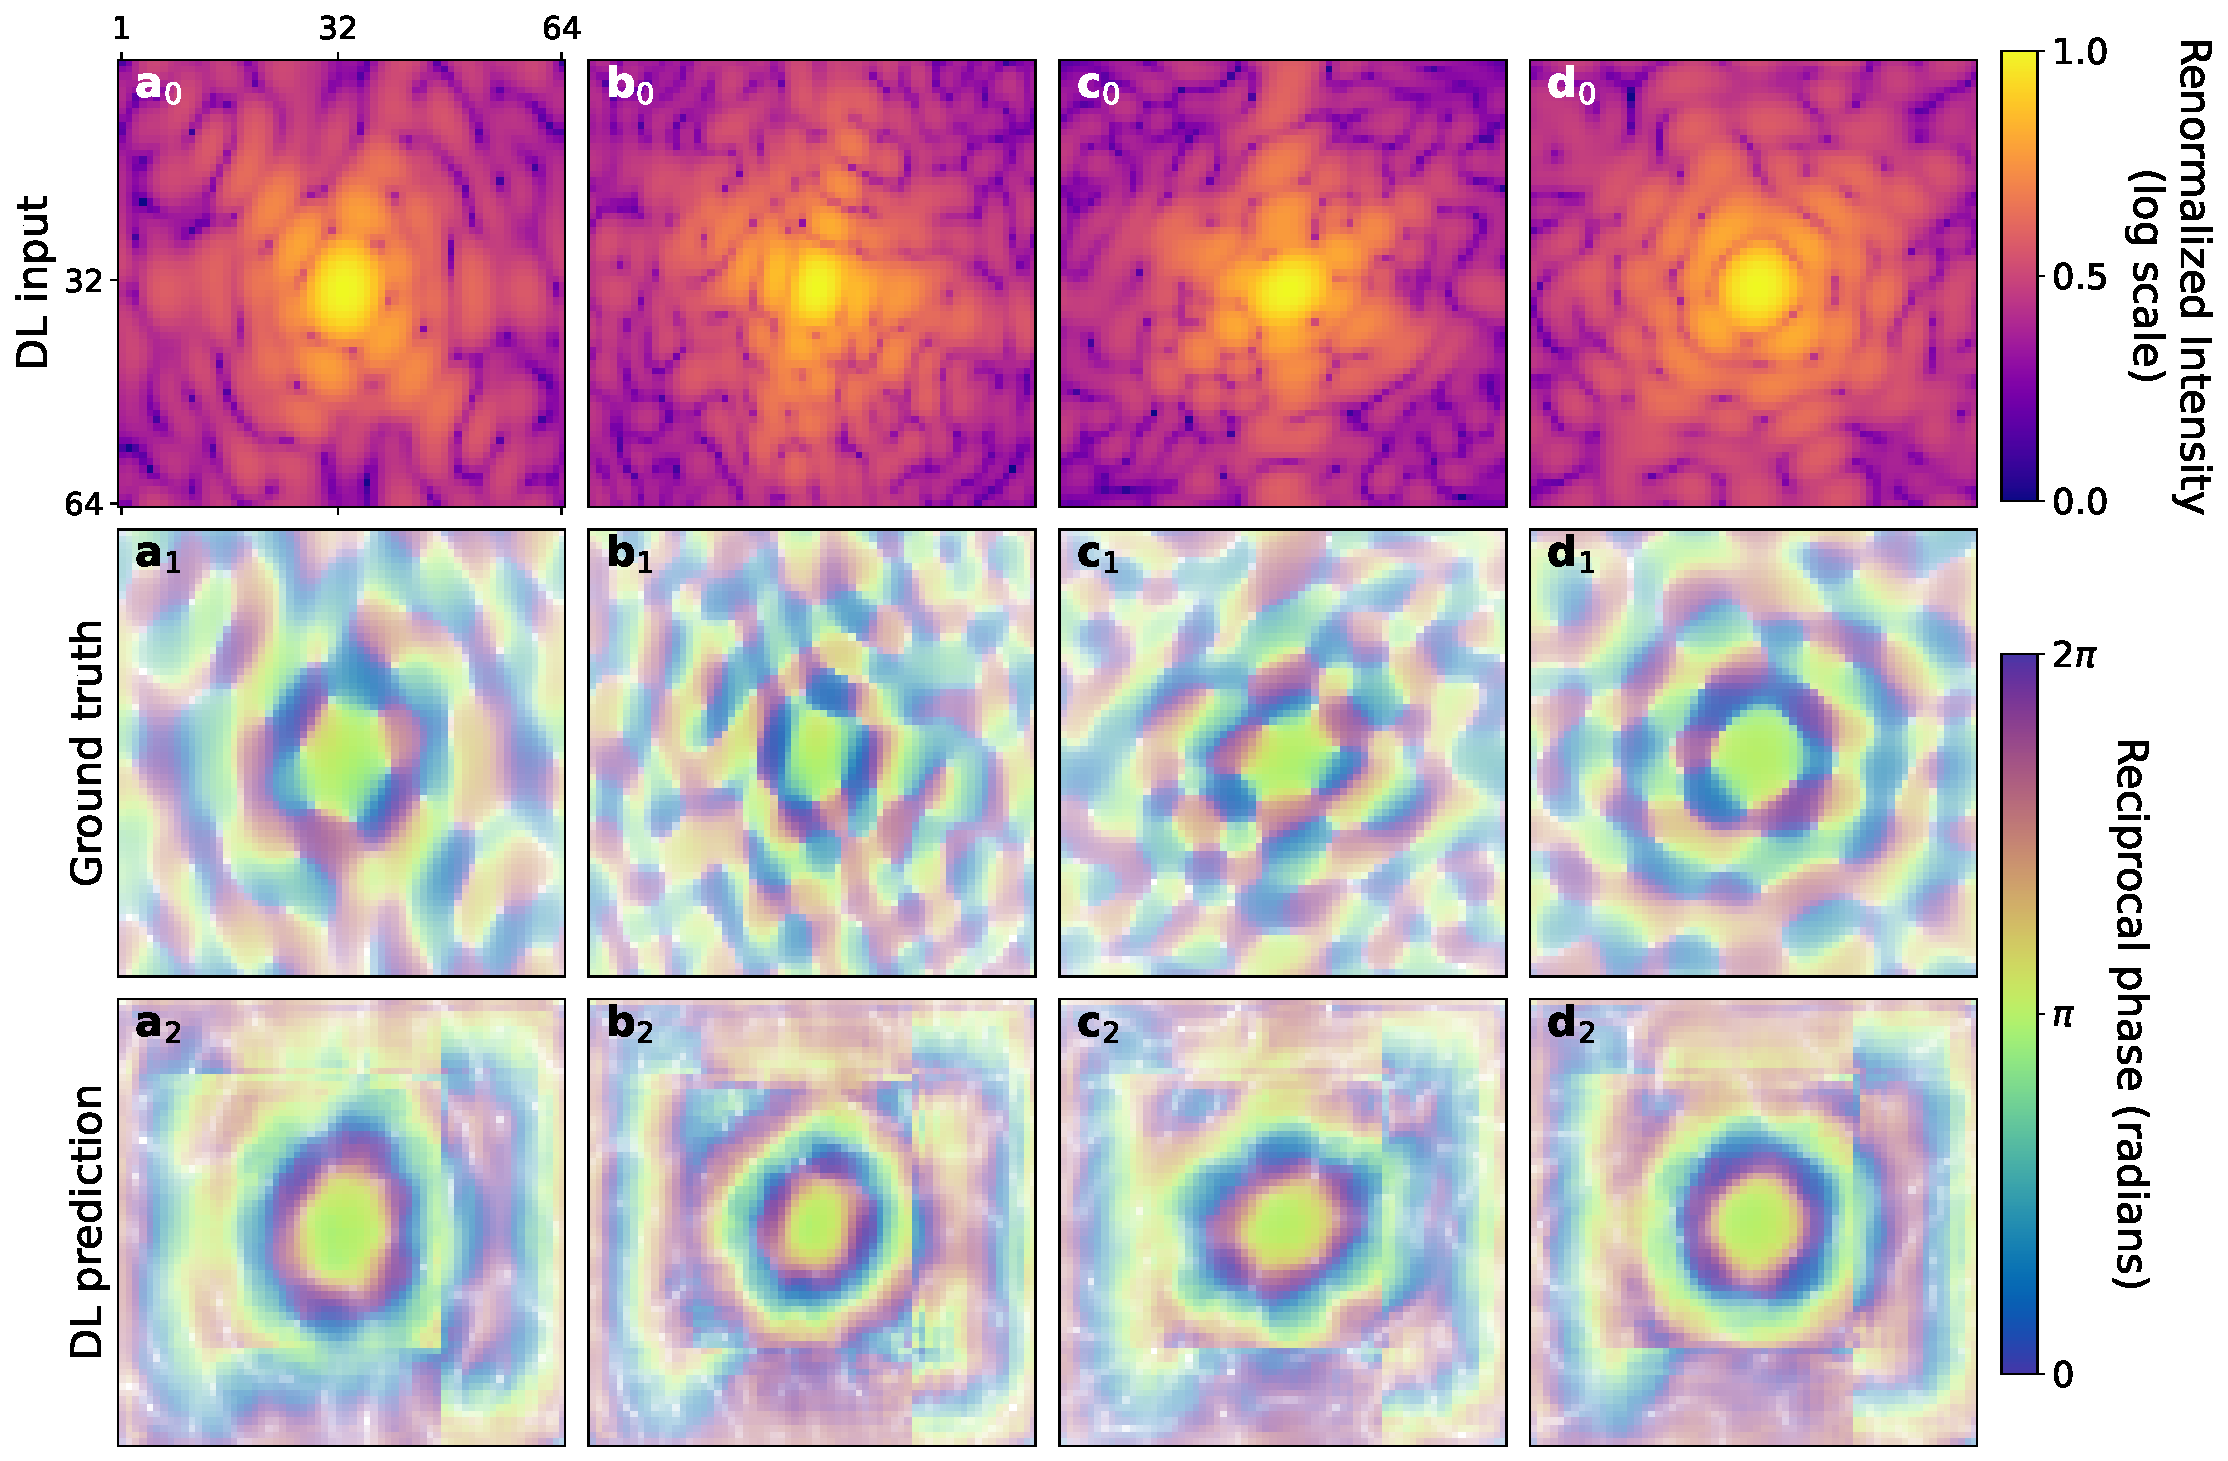
\includegraphics[width=.8\textwidth]{figures/Phasing/RSP_low_strain_doubleMSE_symmJuSun.pdf}
    \caption{\textbf{Model testing using MSE loss function and biased dataset}. First row shows four simulated BCDI patterns, second row the ground truth RSP 
    corresponding to the pattern and last row the DL prediction }
    \label{fig:RSP_lowStrain_doubleMSE_JuSun}
\end{figure}

\begin{figure}[H]
    \centering
    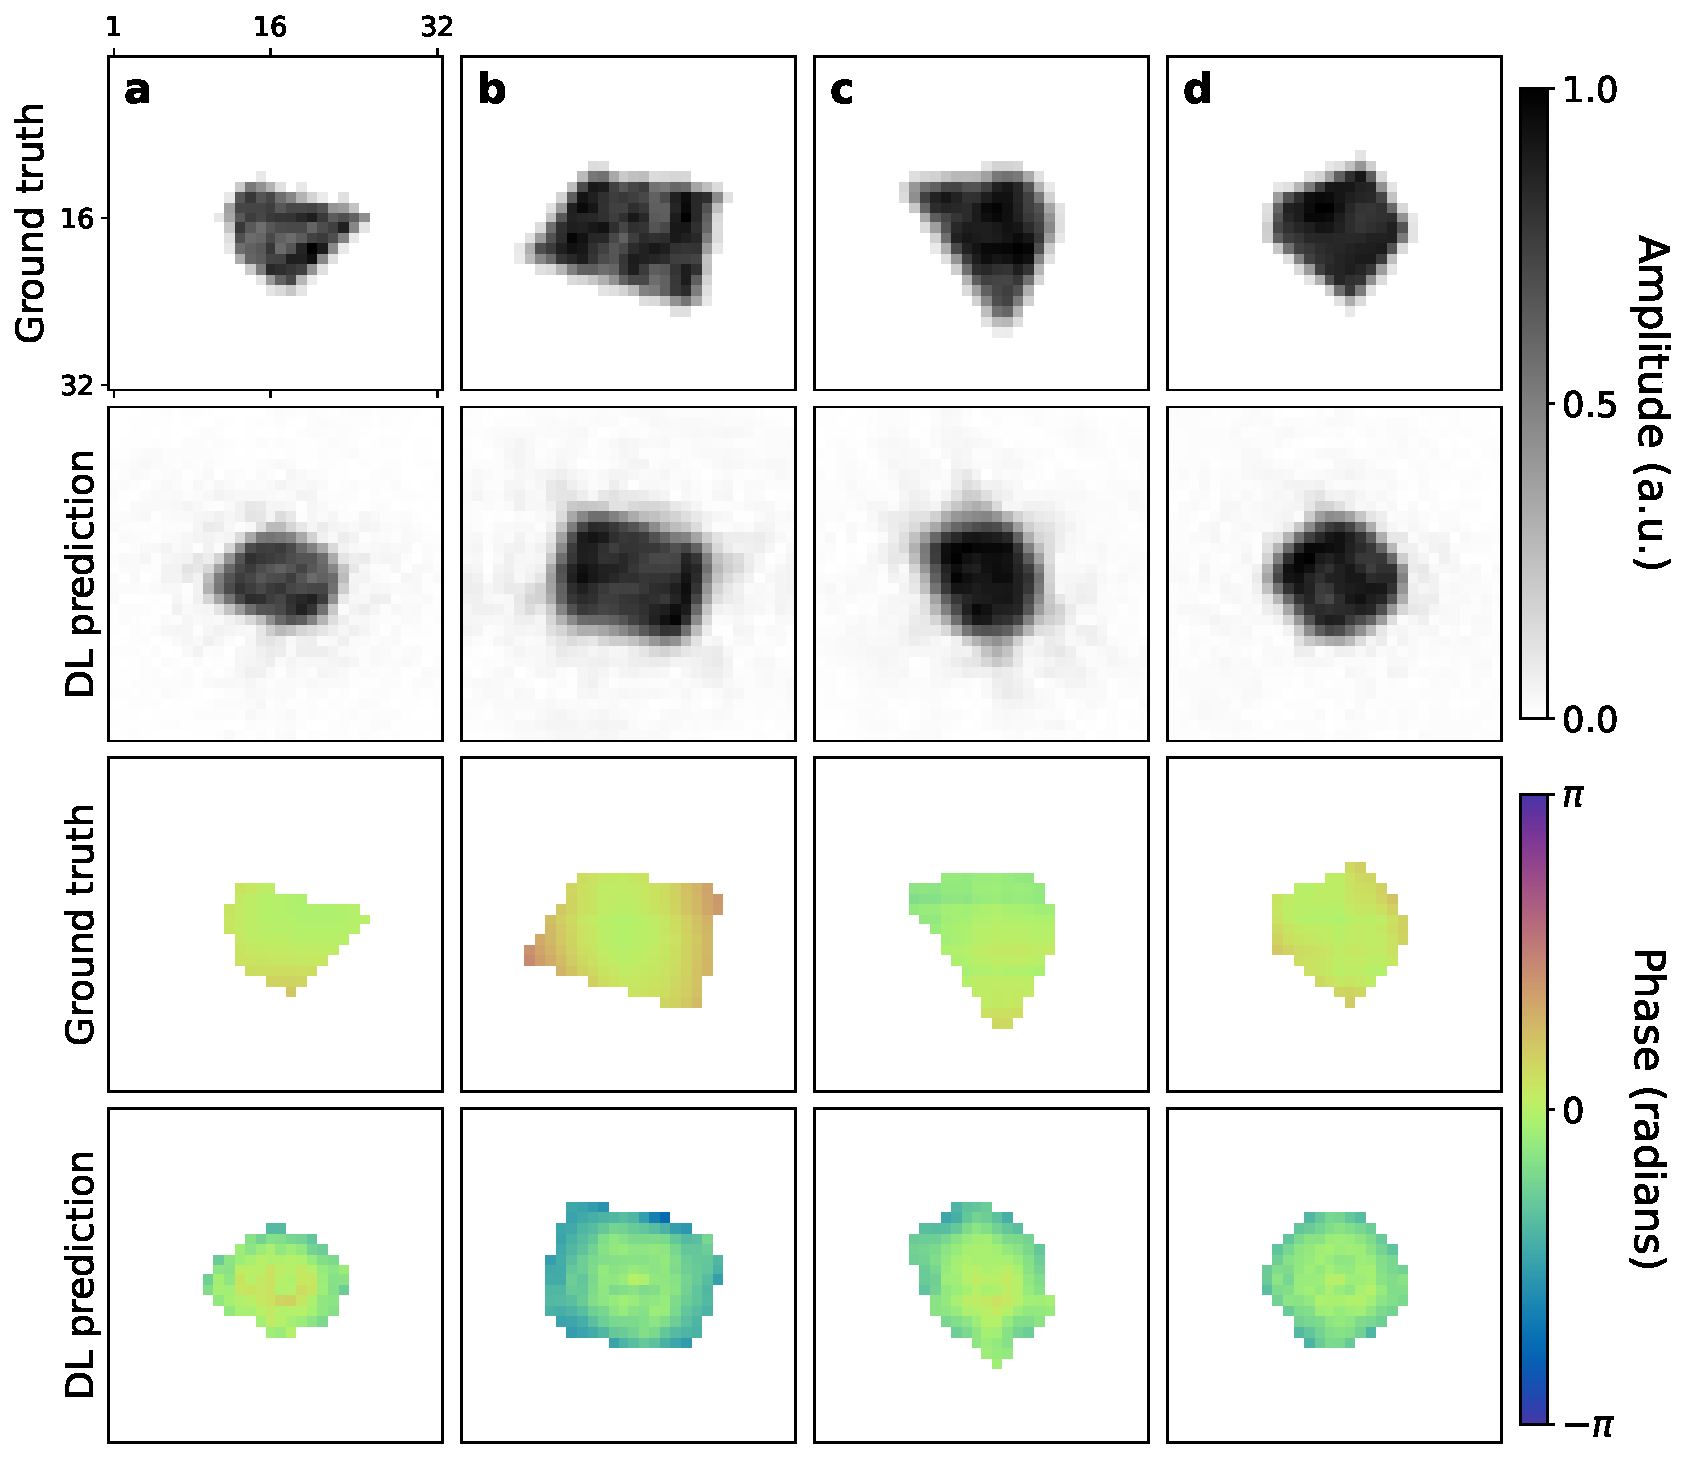
\includegraphics[width=.8\textwidth]{figures/Phasing/obj_low_strain_doubleMSE_symmJuSun.pdf}
    \caption{\textbf{Corresponding reconstructed objects}. Ground truth and predicted objects' amplitudes (first two rows 
    respectively) and ground truth and predicted objects' phases (first two rows respectively). No significant improvement 
    can be observed after the adopted sing-symmetry breaking procedure.}
    \label{fig:obj_lowStrain_doubleMSE_JuSun}
\end{figure}

Unfortunately, the proposed method did not seem to solve the sign ambiguity of the RSP. The model is still unable to 
discriminate between the plus/minus sign of the RSP and the result is the incorrect overlap of the object with its twin
obtained by the inversion symmetry. The phase, though small for this case, is also showing a kind of centro-symmetry 
as its variations tend to spread radially from the center of the array. 

\subsection{The Weighted Coherent Average loss function}
At this point in the study, and in anticipation of applying the model to portions of the RSP, it became necessary to 
consider a loss function that would operate directly on the phase, without requiring transformations into real space. 
However, the main challenges were posed by the symmetries inherent to the phase. Upon further reflection, it was concluded
that a Mean Squared Error (MSE) is not an appropriate metric for comparing the phases of complex functions. Indeed, MSE 
fails to account for the 2$\pi$ periodicity and the possibility of a global phase offset. One could argue that 2$\pi$ wraps 
can be fixed with a modulo 2$\pi$ operation and the offset can be removed by shifting the tensor by a constant. However, 
the modulo wrapping function jumps abruptly by 2$\pi$ every time phase crosses an integer multiple of 2$\pi$, meaning that 
the gradients are infinite thus not advised for gradient-based optimizations. Moreover, the MSE (or MAE and other 
\textit{divergent} metrics) will have problems at the 0-2$\pi$ boundary. In fact, when considering the phase mapped in the
0-2$\pi$ range, if we suppose a $\varphi_{pred}^0 = -0.1$ where $\varphi_{G.T.}^0 = 0$, the wrap will move the $\varphi_{pred}^0$ to the value 
$2\pi - 0.1 = 6.183$ amplifying the error ( $\Delta )$ from $0.1^2$ to $6.183^2$ improperly.
\\
In order to bypass these shortcomings a new loss function was designed. Here it follows the reasoning process that leads
to the mathematical expression of the loss. \\
The best way to account for the periodicity and the wrap without discontinuities 
and error unbalances, is to evaluate the ground truth - predicted phase differences ($\Delta_k$) on the unit circle. 
To do such, it's necessary to express $\Delta_k$ as angles of a complex exponential. This means that if $\varphi_{pred}$ is an array of 
random values, each complex number $ z_k = e^{(i\Delta_k)}$, when represented on the Argand plane, can be seen as a 
vector pointing at a random coordinate on the unit circle. Now, the goal of the optimization is not to minimize $\Delta_k$ 
for all $k$ but to have the same $\Delta_k$ throughout $k$. In fact, for $\varphi_{pred} \Leftrightarrow \varphi_{G.T.}$ each 
vector $z_k$ points in the same direction, but it does not necessarily lie on the x-axis ($\Delta_k = 0 $ condition). 
Therefore, the loss function should ultimately drive all the $z_k$ from randomly distributed to coherently aligned along a common 
direction. A helpful quantity in this case can be the complex average vector $\langle z \rangle = \sum_{k=1}^{N}z_k = \sum_{k=1}^{N}e^{(i\Delta_k)}$
where $k$ runs over all the $N$ pixels. In particular the length of $\langle z \rangle$ , represented by the modulus $|\langle z \rangle|$,
is an efficient metric for the measurement of the degree of ``coherence'' among all the complex phase differences. 
In fact, $|\langle z \rangle|$ scores 0 for randomly oriented $z_k$, as opposite contributions cancel out each other because 
incoherent, while it scores 1 for perfectly aligned ones. It follows that one wants to maximize $|\langle z \rangle|$ during the 
optimization. Moreover, given the natural normalization between 0 and 1 of this metric, it follows naturally that the loss 
function can be expressed as $ L =  1 - |\langle z \rangle| $. \\
Additionally, an importance mask can be applied during the averaging process. In particular, we know that the brightest 
pixels of the BCDI pattern are the ones contributing the most to the object's reconstruction. For this reason one could 
weigh the complex average multiplying by the input magnitudes. The effect of this operation is to ``give a direction'' to the 
optimization, meaning that the $\langle \Delta \rangle $ the model will tend to converge to, will be mostly steered close to 
the $\Delta_k$ of the brightest $k$ pixels. 
The loss can now be expressed as: 

\begin{equation}
    L = 1 - \left|\frac{1}{N}\sum_{k=1}^{N} \sqrt{I_{k}}\exp\left(i(\varphi_{\text{GT},k} - \varphi_{\text{pred},k})\right)\right|
\label{eq:WCA_1}
\end{equation}

Where $N$ is the total number of pixels in each RSP array and $k$ is the pixel index. $\sqrt{I}$ is the magnitude of the BCDI pattern 
normalized between 0 and 1 with respect to the sum, and $\varphi_{\text{GT}}$ and $ \varphi_{\text{pred}}$ the ground truth and 
predicted RSP. \\
The last missing piece is the removal of sign symmetry. Rather than biasing the dataset preferring one sign over the opposite, 
the function $L$ is computed for both $\varphi_{\text{GT}}$ and $-\varphi_{\text{GT}}$ and in a second passage, the minimum of the two 
along the batch dimension is kept for backpropagation. The final form of the Weighted Coherent Average (WCA) loss is then given 
by: 

\begin{equation}
    L_{\text{WCA}} = \min\left(L_+, L_-\right)
\label{eq:WCA_2}
\end{equation}

To better visualize the functioning of the WCA loss function, a simple model has been trained to fit the ground truth phase 
of a single 2D BCDI pattern using the WCA. The complex phase differences vectors were extracted at each step of the optimization 
together with the updates obtained from the gradients of the WCA with respect to the trainable parameters. Fig. \ref{fig:WCA} 
shows the evolution of the predicted RSP as well as the progressive alignment of the  $z_k$.
\begin{figure}[H]
    \centering
    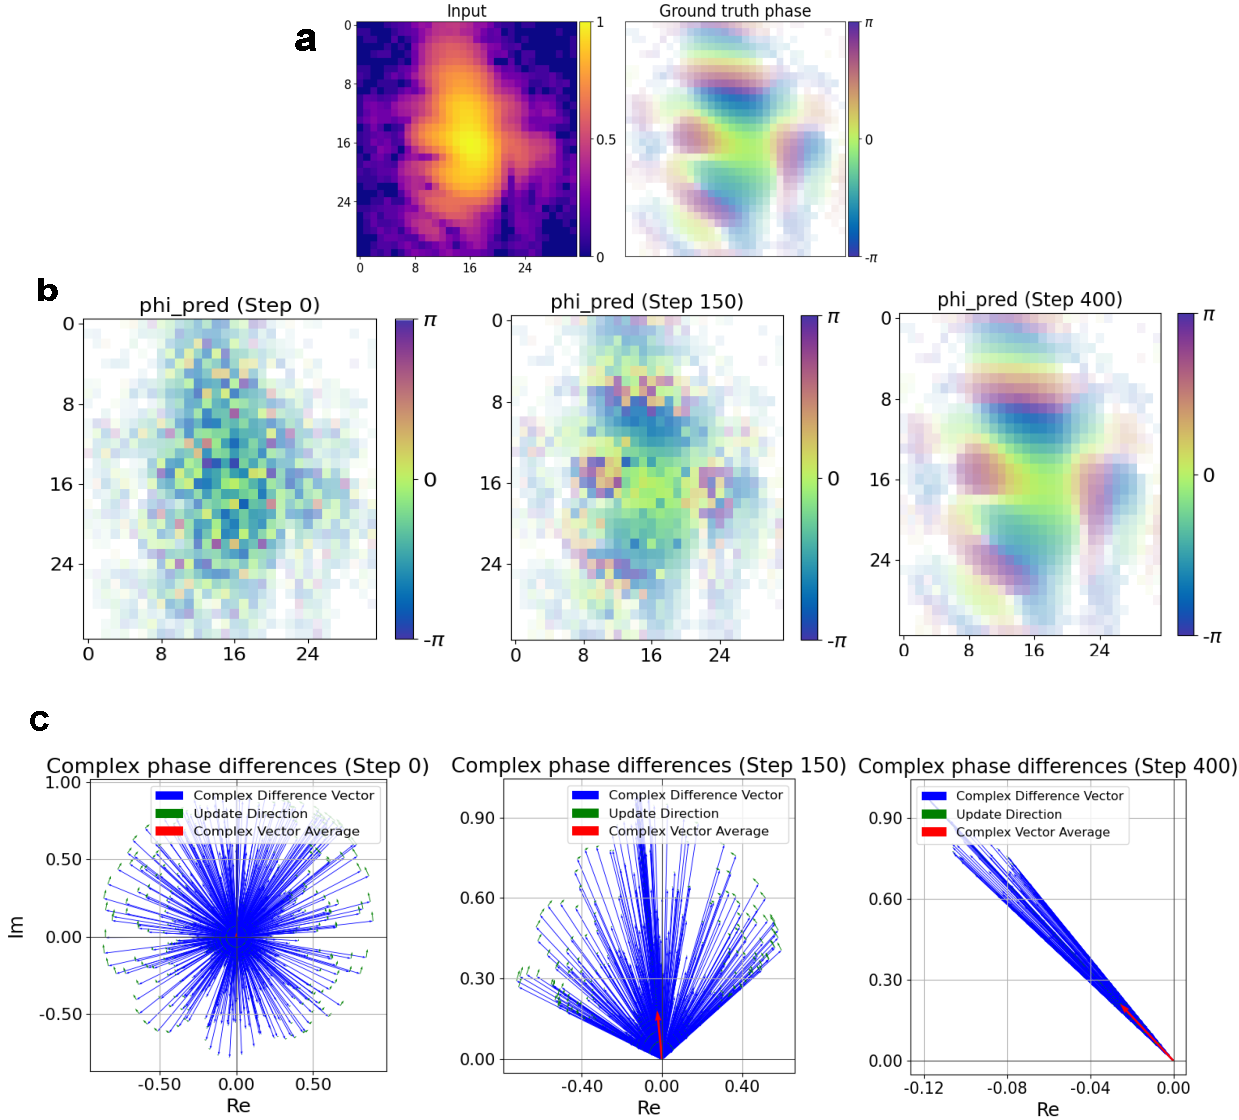
\includegraphics[width=.8\textwidth]{figures/Phasing/WCA.pdf}
    \caption{\textbf{Illustration of the WCA loss function}. \textbf{a} Input intensity (log-scale normalized) and
    ground truth RSP. \textbf{b} Predicted RSP in steps 0 - 150 - 400 of the optimization. \textbf{c} Corresponding 
    complex phase-differences vectors $z_k$ on the Argand plane (blue arrows), together with the updates (green arrows) obtained 
    from the gradients of the WCA, and the resultant complex average $\langle z \rangle$ (red arrow). It is visible that 
    during the fit, as the $z_k$ align around a common one, the amplitude of $\langle z \rangle$ grows bigger and the predicted 
    RSP converges to the ground truth one.}
    \label{fig:WCA}
\end{figure}

The same model has been trained using the WCA for the same number of epochs on the same dataset and here the results are 
shown. First, it can be noticed in Fig.\ref{fig:loss_vfn} that the training and validation loss values throughout the 
training are following different trends with respect to the model trained with the MSE loss (Fig. \ref{fig:loss_2mse_nosymm})

\begin{figure}[H]
    \centering
    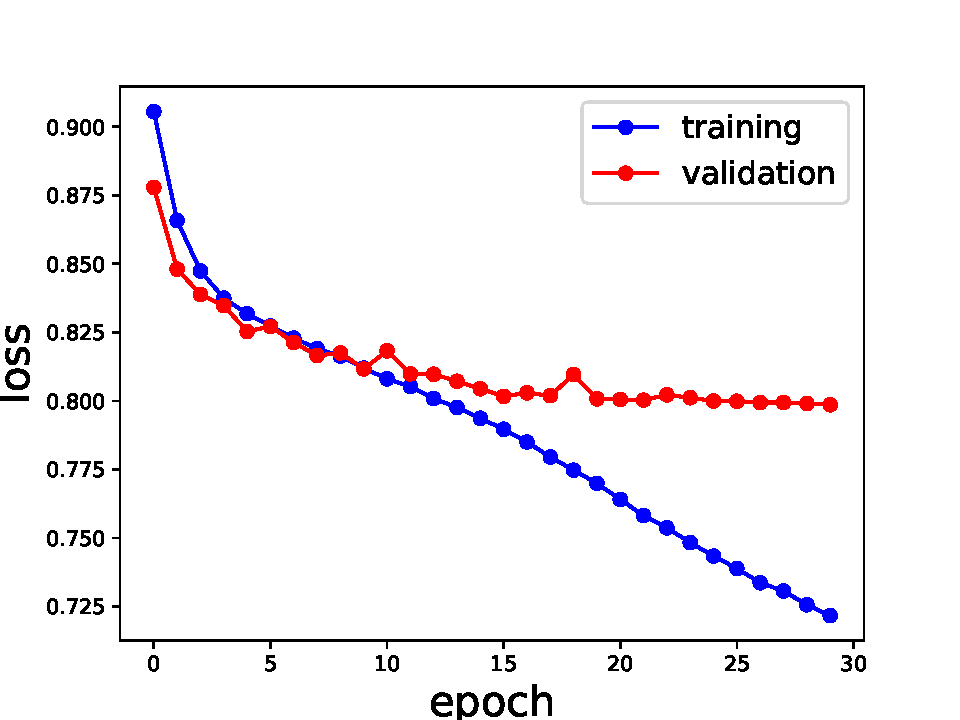
\includegraphics[width=.8\textwidth]{figures/Phasing/loss_low_strain_noiseless_doubleVFN.pdf}
    \caption{Training and validation loss curves over 60 epochs.}
    \label{fig:loss_vfn}
\end{figure}

In this case the correct learning curve does not reach a plateau within the first 25 epochs but maintains a negative slope 
for longer, indicating a better learning. This suggests indeed better results when used on test data. 
In particular, for the same input diffraction patterns tested above in Figs.\ref{fig:RSP_lowStrain_doubleMSE_JuSun} - \ref{fig:obj_lowStrain_doubleMSE_JuSun}
the model trained with the WCA yields the prediction shown in Fig.\ref{fig:RSP_vfn} for the RSP and Fig.\ref{fig:obj_vfn} 
for the corresponding reconstructed objects. 

\begin{figure}[H]
    \centering
    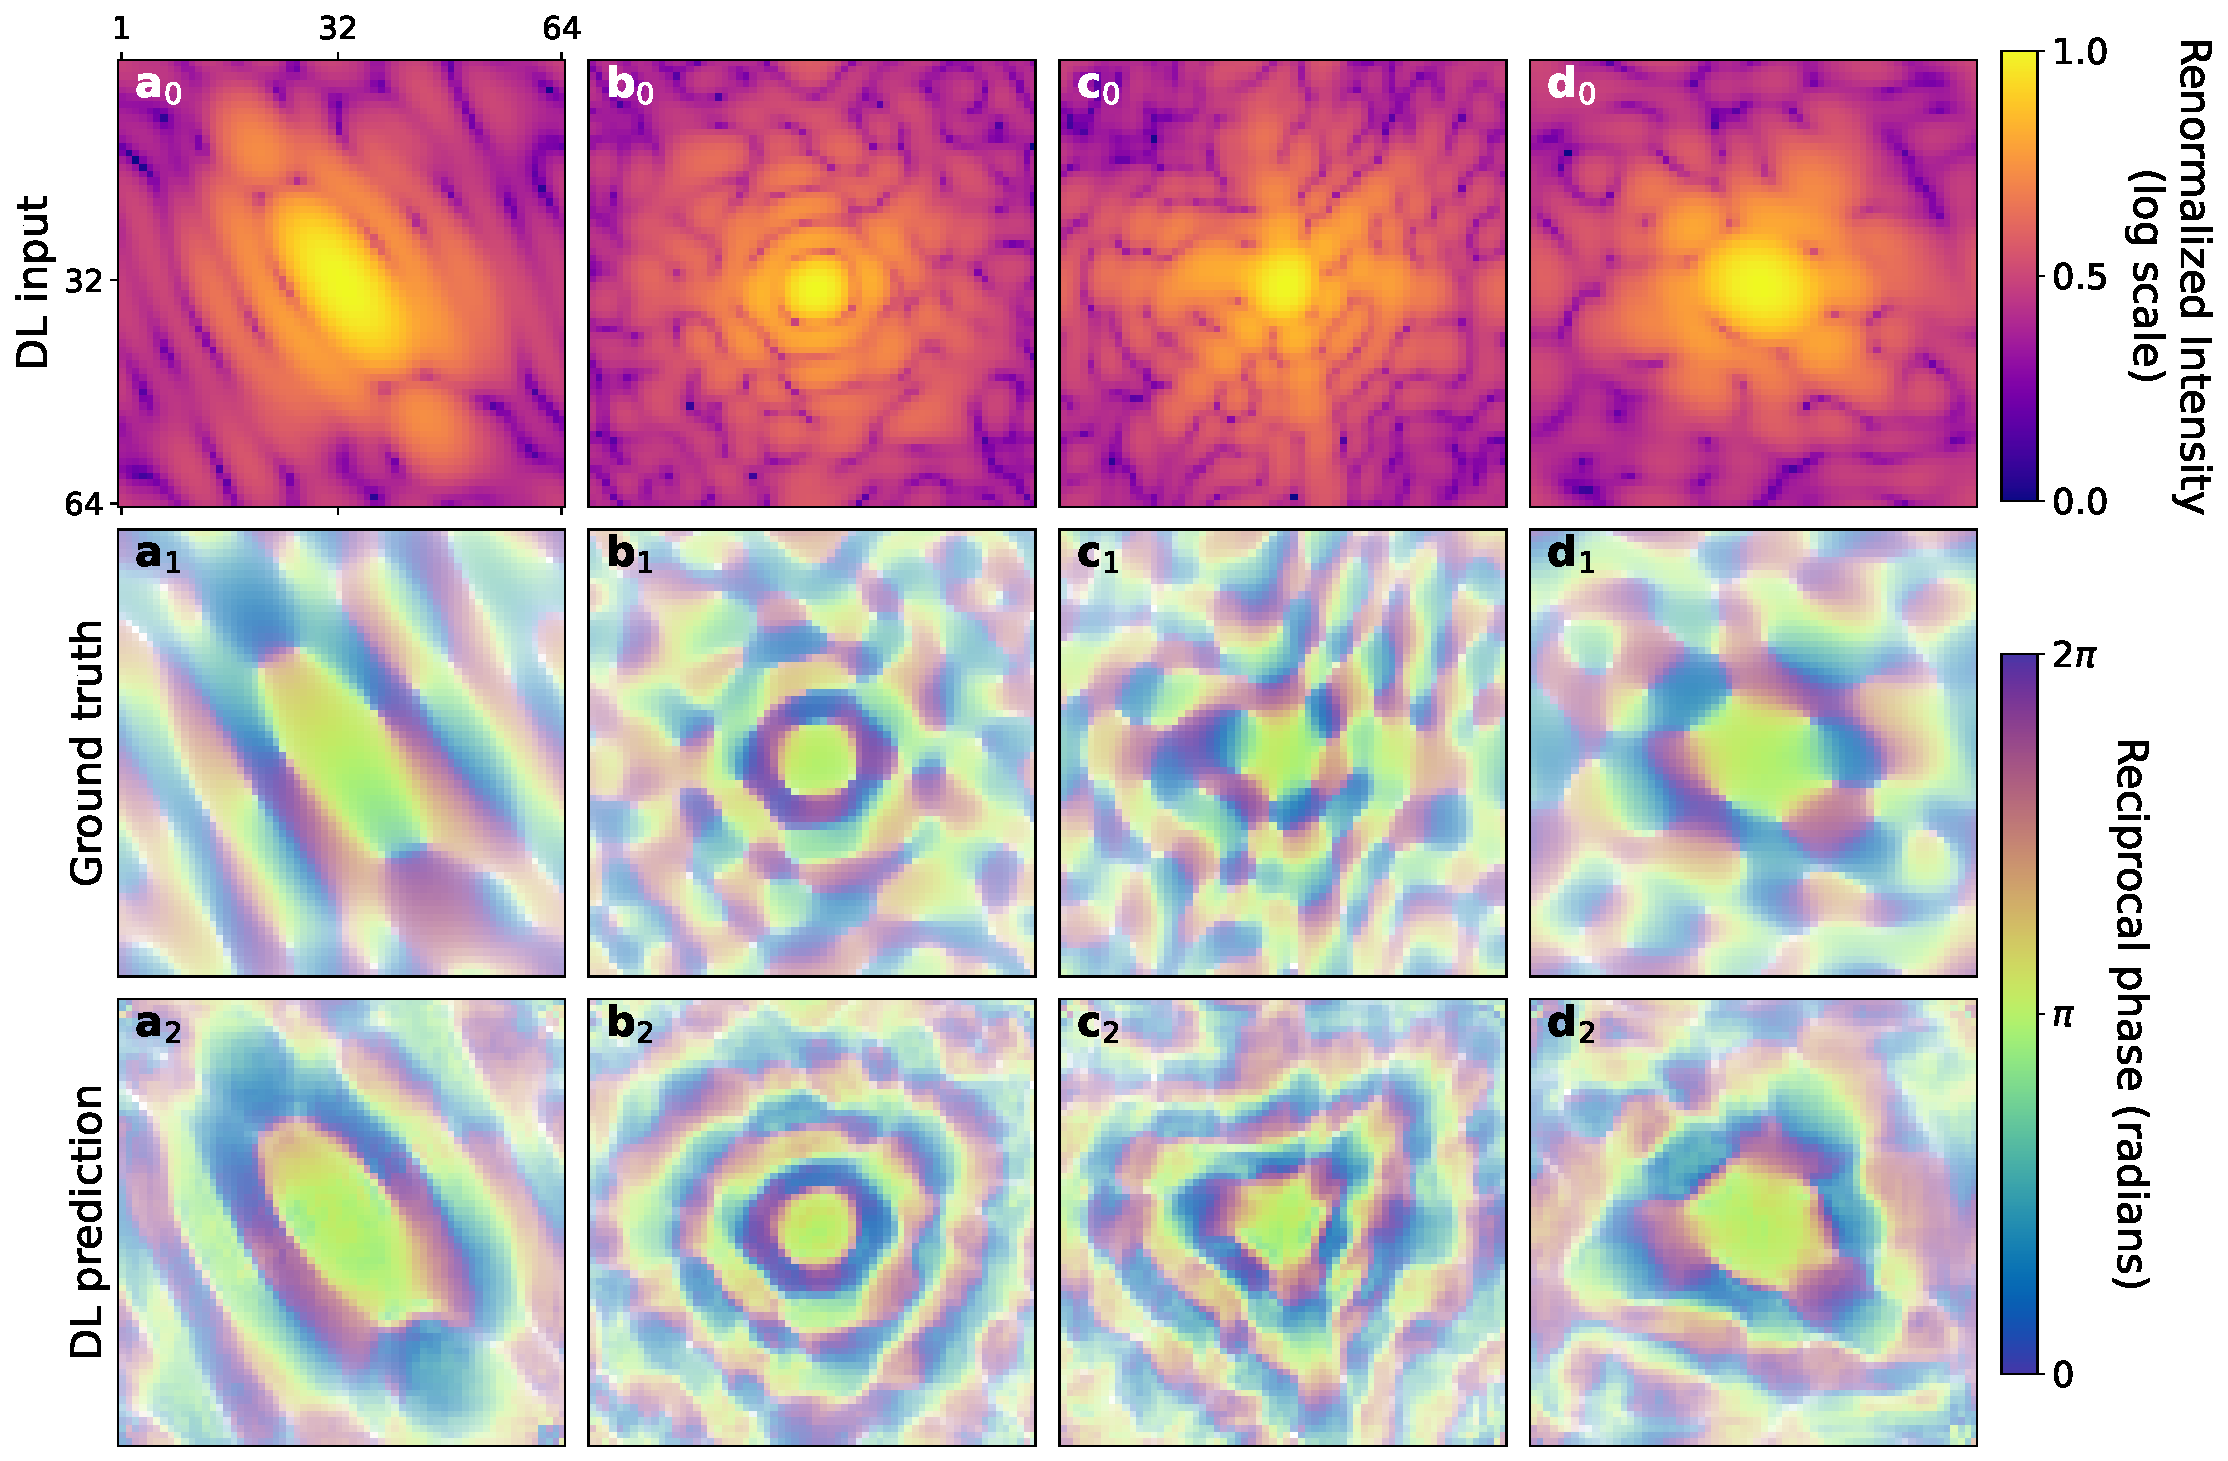
\includegraphics[width=.8\textwidth]{figures/Phasing/RSP_low_strain_VFN.pdf}
    \caption{\textbf{Model testing using WCA loss function}. First row shows four simulated BCDI patterns, second row the ground truth RSP 
    corresponding to the pattern and last row the DL prediction }
    \label{fig:RSP_vfn}
\end{figure}
\begin{figure}[H]
    \centering
    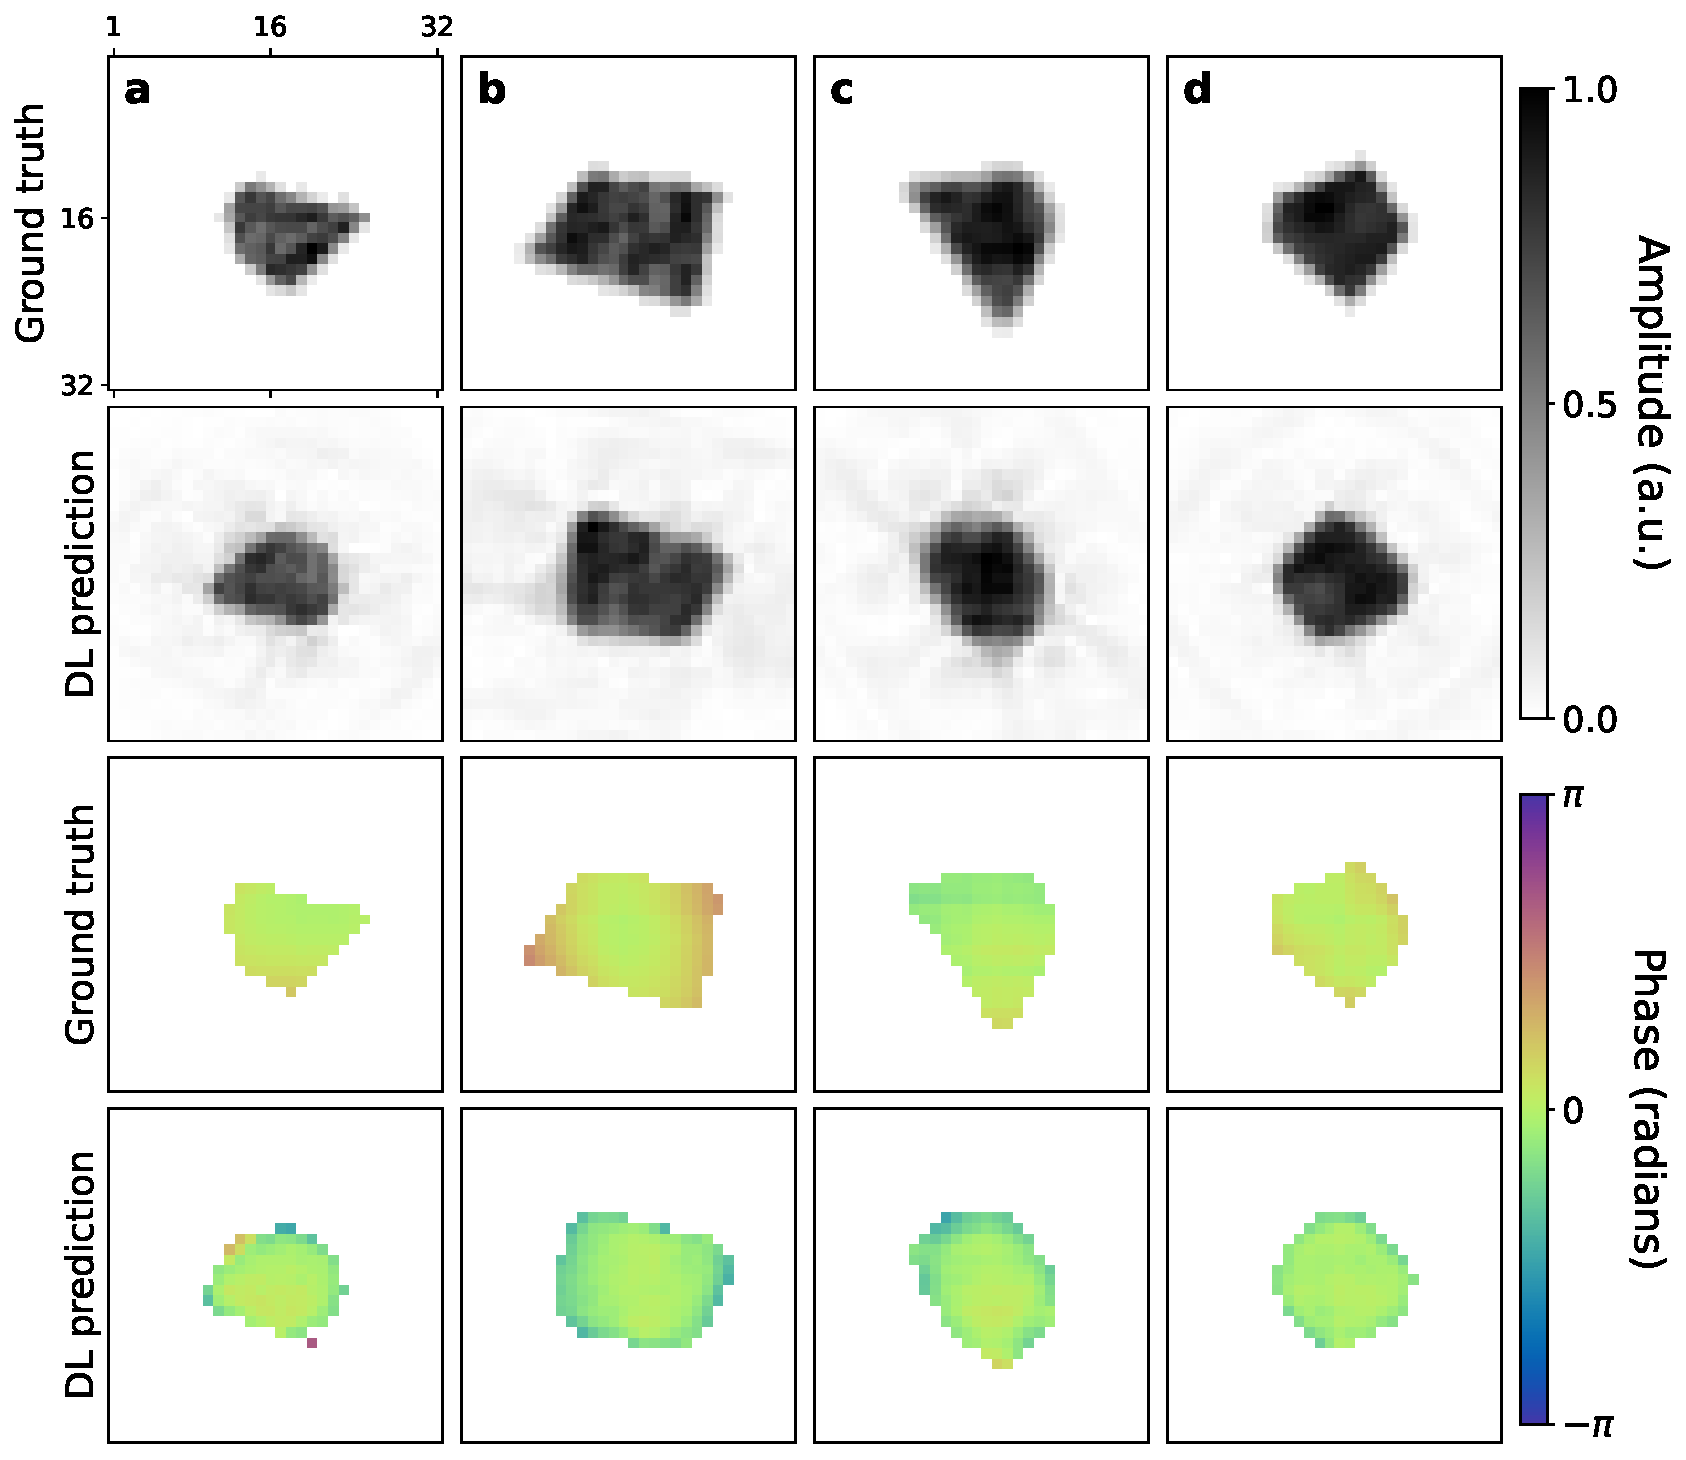
\includegraphics[width=.8\textwidth]{figures/Phasing/obj_low_strain_VFN.pdf}
    \caption{\textbf{Corresponding reconstructed objects}. Ground truth and predicted objects' amplitudes (first two rows 
    respectively) and ground truth and predicted objects' phases (first two rows respectively). }
    \label{fig:obj_vfn}
\end{figure}

The results obtained from the model trained with the WCA loss function are visually better than the MSE ones. Although not 
completely removed, the sign symmetry that gives rise to the superposition of the object with its twin, is less pronounced. 
For example, particles in Fig. \ref{fig:obj_vfn}(a-b-d) have a clear orientation and a shape that matches the ground truth. 
In all those cases though, the model has opted for the conjugate solution as the predicted object are flipped with respect to 
the ground truth ones. In Fig. \ref{fig:obj_vfn}(c) instead the symmetry is not broken and the result is still a superposition 
of the particle with its twin. This suggests that the symmetry breaking method implemented in the WCA, and the one proposed by 
Zhang and coauthors, is only partially playing a role in the actual model learning. It is interesting to notice indeed that 
when the training dataset or the model trainable parameters are increased, the sign symmetry is completely removed in the most 
difficult cases as well. Fig. \ref{fig:loss_comparison} shows the effect of the dataset and models sizes for both MSE and WCA 
loss functions on the same simulated test data. The first important piece of information this figure shows is that the model trained 
with the WCA reaches higher accuracy. Moreover, it is much faster to compute since no FFT or IFFT is involved, thus the training time 
is drastically reduced. For what concerns the accuracy metric, in order to properly account for both modulus and phase, 
it has been calculated using 
\begin{equation}
 \left(\frac{PCC(m) + WCA(\varphi)}{2}\right)\times 100
\end{equation}
where $PCC(m)$ is the Pearson Correlation Coefficient on the object's modulus and $WCA(\varphi)$ is the WCA function 
applied to the object's phase inside the support. For what concerns the sign symmetry problem it is evident that while for 
the MSE trained model it is resolved only for a larger number of trainable parameters, for the WCA trained one it is already 
sufficiently overcome. As last observation, it is interesting to notice that when the model size is kept fixed and the training 
dataset augmented, the WCA improves the performances while for the MSE it is not the case. 

\begin{figure}[H]
    \centering
    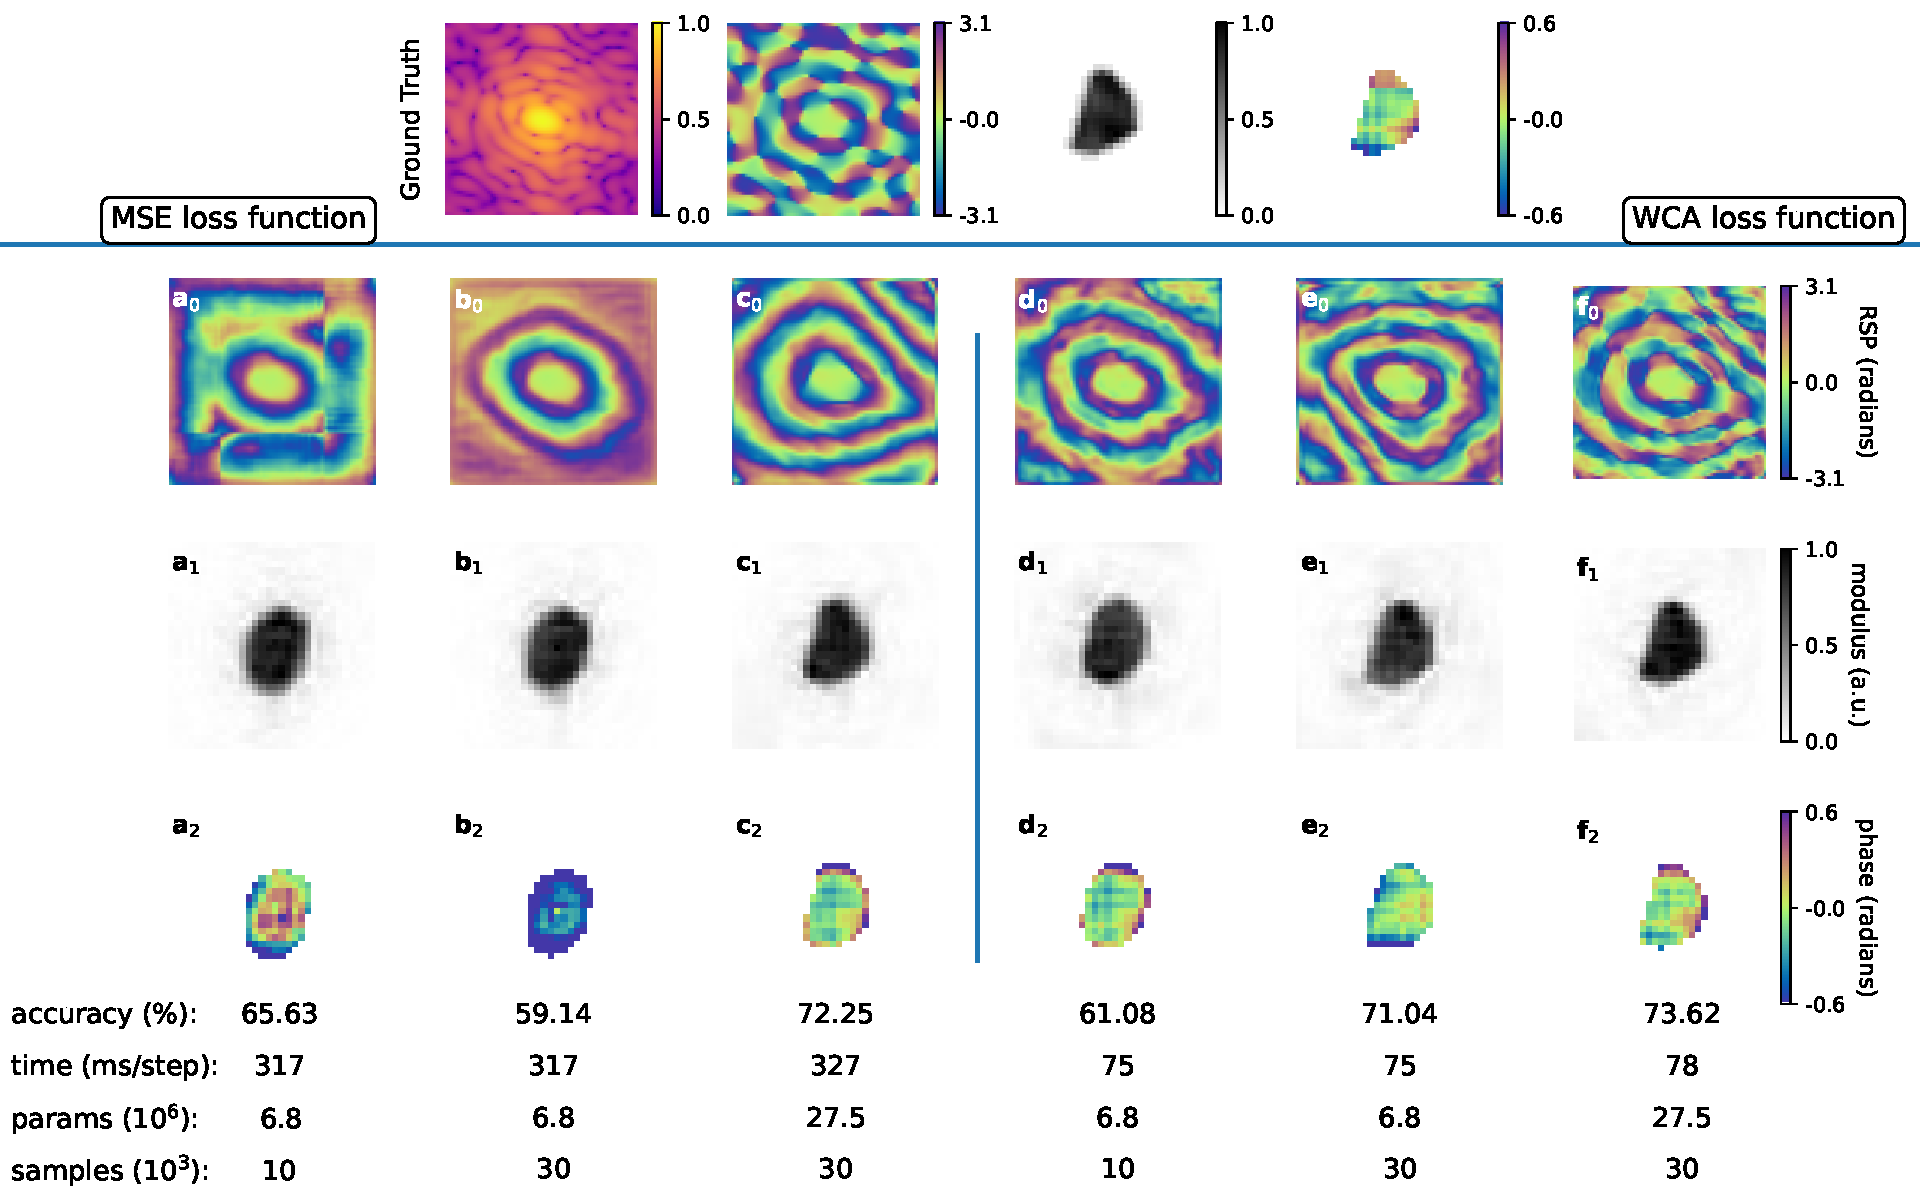
\includegraphics[width=\textwidth]{figures/Phasing/model_comparison.pdf}
    \caption{\textbf{Comparison of MSE and WCA loss function for different model and training dataset sizes} In the first 
    row from left to right the input intensity, the ground truth RSP and the corresponding object (modulus and phase) are 
    represented. \textbf{$a_0, b_0, c_0$}} are the results of the predicted RSP obtained from the model trained with the 
    MSE loss function with the initial number of parameters and training set (\textbf{a}), with the augmented dataset (\textbf{b})
    and with both model and dataset size increased (\textbf{c}) In third and fourth rows the corresponding reconstructed 
    objects are displayed. \textbf{$d, e, f$} columns symmetrically shows the results obtained with the model trained using the WCA loss. 
    \label{fig:loss_comparison}
\end{figure}


The preliminary studies on the 2D case for low-strain particles have demonstrated the possibility to recover the RSP from 
the diffracted intensity pattern with a U-Net like architecture without ever calculating the object in real space.
From these promising results, it was decided to investigate the mapping intensity-RSP for portions of the reciprocal space. 


\section{Phasing patches: 3D case low strain}\label{chp:patches_nostrain}
% MODEL 3D CASE NO STRAIN WITH PATCHES: SHOW THE MODEL WITH DIFFERENT WCA LOSS FUNCTION 
In this section of the manuscript the DL prediction of ``patches'' of the RSP will be explored and discussed. 
Three-dimensional BCDI pattern of low strained particles were used to conduct this study. 
Although this patching approach has not given satisfactory results for the PR, it is nevertheless reported in the manuscript as 
study on the \textit{local} rather than \textit{global} relationship between the diffracted intensity and the RSP. It is 
indeed known that there exist a unique mapping, barring some trivial RSP symmetries, between the diffracted intensity 
and the RSP in 3D \cite{Miao:98}. What is interesting to investigate is whether this relationship exists also for subsets 
of the reciprocal space, and in particular if it can be retrieved by a DL model. (From now on the term ``patches'' 
will be used to refer to cubic subsets of the reciprocal space). \\

When deciding to work with patches, there is a number of questions that arise and the answer to which is not 
straightforward nor unique in many cases. Namely: What size is best? Can the patches 
be extracted at random positions or should there be an order? What about the normalization of the intensity range inside 
the patch? How are the patches stitched together into the full RSP eventually? How are the phase symmetries taken into account 
during the stitching? 
Here I will present the approach that allowed me to address these questions. 

\subsection{The choice of the size}

Similarly to the inpainting case, 32 pixel-side cubic patches, cropped out of 128 pixel-side simulated
BCDI patterns were considered. The choice is supported by the following reasons: 

\begin{itemize}
    \item The good results obtained for the inpainting case suggested that the amount of information contained inside a
    32 pixel-side patch of reciprocal space is enough for the model to grasp spatial correlations.  
    \item The average oversampling ratio of BCDI experimental data is such that in a 32 pixel-side volume a sufficient
    amount of fringes is contained, meaning intuitively that the model can predict the corresponding RSP. 
    \item An even number multiple of 2 is usually considered GPU-friendly since it facilitates the shared calculations across
    different threads. 
\end{itemize}

\subsection{Patches division and stitching}
At first, the patches were thought to be extracted randomly from the full BCDI pattern as for the inpainting case. 
However, by doing so the RSP of each patch would in principle have different offsets and different wraps than the neighbors 
and this would complicate the stitching of the patches back into the full RSP. 
For this reason, and considering the approximate spherical symmetry of the average BCDI pattern it was decided to crop patches radially, 
starting from the region around the center of the Bragg peak and the progressively moving outwards to higher q-values. 
In this configuration, an integer step (10 pixels in our case) was chosen beforehand and the first patch around the center 
of the Bragg peak was selected together with all the patches centered in distances of integer multiples of the chosen step. 
Fig. \ref{fig:patches_cropping} shows a simplified schematic of the patches extraction. 
For the DL model training the patches of the intensity pattern need to be selected as well as the for the corresponding 
RSP for ground truth comparison. 


\begin{figure}[H]
    \centering
    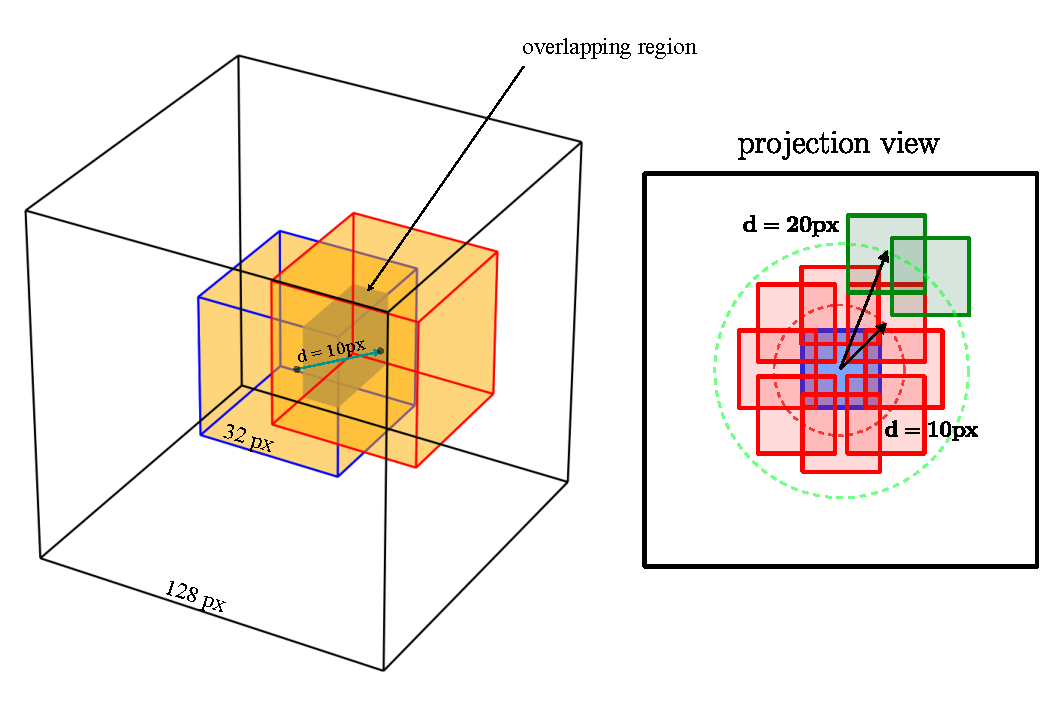
\includegraphics[width=\textwidth]{figures/Phasing/patching_cropping.pdf}
    \caption{Schematic of the cropping of patches. From the full BCDI pattern (white 128 px-sided cube) the first patch is 
    cropped out in the center and (orange 32 px-side cube with blue outline). Other patches are extracted radially from 
    concentric shells separated by a 10 pixels step. Here only one patch from the first shell at distance 10 pixels from the 
    center of the peak is displayed for simplicity. The gray shaded area highlights the overlapping volume between the 
    two patches. }
    
    \label{fig:patches_cropping}
\end{figure}

Being the step size smaller than the 
semi-diagonal of the 32 pixel-sided patches, it follows that the patches of adjacent cells have overlapping volumes. 
These common regions can have a twofold purpose. Firstly, they reduce the complexity of the stitching procedure since 
when this is executed progressively starting from the central patch, the sign and the offsets of the RSP are unambiguously 
fixed for all the following ones. Secondly, during the DL model training, for patches belonging to the outer shells, 
the overlapping volume of RSP belonging to the innermost adjacent shell can be provided as initial guess along with the input 
intensity patches. This of course cannot be exploited for the central patch that necessarily has to be predicted without 
initial RSP guesses. \\
The last question to be answered concerns the normalization. Since each patch is processed independently of the others 
by the DL model, it was decided to normalize each patch between 0 and 1 (always in log scale). 

To summarize, the final design implied the use of two distinct training datasets and two different CNNs. 
The first dataset was dedicated to the central portion, therefore the first CNN was provided with 3D intensity patches in 
input (normalized log scale) and corresponding RSP patches as ground truth labels. A second training dataset containing 
patches from outer shells (5 concentric ones for a 128 pixel-sided full BCDI pattern) was created. Here each file was made 
of the pair intensity-RSP initial guess - from the closest neighbor patch belonging to the innermost shell -  as input,
and the full RSP ground truth patch corresponding to the input intensity. This second dataset was used to train a second 
CNN identical to the first one. One observation regarding the datasets is that there is an intrinsic imbalance between the 
number of central patches and the outer ones. In fact, for a single full BCDI pattern, the number of patches in the first shell is 1, 
while the number of outer portions can go up to several hundreds. Moreover, the central patch is the most important one as it 
contains a low resolution representation of the particle in real space. In order to balance the training, the first dataset was 
augmented with more simulated data. 

% add figure with the patches X,y

\subsection{Model architecture}\label{chp:3d_patch_model} 
The model architecture is similar to the one used for the inpainting case, with a U-Net like structure



\section{Patches: 3D case high strain}\label{chp:patches_strain}

% MODEL 3D CASE STRAIN WITH PATCHES: SHOW THE FAILURE AND EXPLAIN WHY 

\section{Model design: 3D case high strain }\label{chp:3d_nostrain}
% MODEL 3D CASE STRAIN FULL DIFFRACTION 

\section{Results on 3D case}\label{chp:phasing}
\section{Refinement with iterative algorithms}\label{chp:phasing}
\section{Experimental results}\label{chp:phasing}



% CHAPTER 6 - Deep Learning for Phase Retrieval
\chapter{Automatic Differentiation for BCDI Phase Retrieval}
\label{chap:AD_phase_retrieval}
% In this last chapter an approach to the BCDI Phase Retrieval based on Automatic Differentiation will be discussed.
% It started from the necessity to 
% Unlke the DL model discussed above this method is iterative and

\epigraph{``An approach that would be superior to the ones considered here would be one that minimizes the Fourier-domain error while inherently satisfying the object-domain
constraints, or one that minimizes an error metric that combines the Fourier- and object-domain constraints [...]. 
Something along these lines would be very useful for the problem of a single intensity measurement; clearly, 
more could be done in this area''}{J.R.Fienup \cite{fienup_phase_1982}}

In this chapter a different approach to the BCDI phase retrieval will be presented. It originated from the need to resolve 
those cases in which neither standard alternating algorithms, nor the DL assisted PR can succeed to converge to a satisfactory 
reconstruction. The developed approach differs from the alternating projections algorithms classically used for 
the Fourier PR, as it is formulated as minimization problem solved with gradient descent (GD). The gradients however are computed 
through the efficient automatic differentiation (AD) enabled by graph-based differentiable programming packages like Tensorflow and 
PyTorch, accelerated on GPU. For this reason one could see the AD approach as unsupervised machine learning on a single training 
dataset.\\ 
The GD - based optimization is fundamentally different from fixed point alternating projections. Here one could qualitatively say 
that if the latter switches between real and reciprocal space applying constraints in both, the former initializes a 
complex object and updates at each cycle its modulus and phase using the gradients, with respect to them, of the differences 
between the observed and calculated diffracted intensities. In this way, the knowledge on the particle can be implemented 
by initializing the object with some physical constraints or adding regularization terms that will drive the updates 
towards more reasonable solutions. \\

% After mentioning the most relevant literature on AD, and more generally GD-based, phase retrieval for CDI, 
% we will present our formulation of the problem and the results obtained on simulated and experimental BCDI patterns. 

\section{State of the Art}
AD methods for PR have been investigated already in 2014 by Jurling and Fienup \cite{Fienup_AD} who first considered the use of 
AD for GD-based PR. In this theoretical work the authors proposed a pedagogical ``manual automatic 
differentiation'' approach for the phase problem, extended to complex-valued variables. The authors also denounced the 
lack of suitable softwares as major limitation to the use of AD-based PR. The advent of high-level, GPU oriented, libraries such 
as Tensorflow, PyTorch, JAX and Autograd has opened the opportunity to efficiently exploit AD algorithms for the phase problem. 
The first implementations in the CDI field have considered mostly ptychography in forward and Bragg geometries \cite{Nashed_2017, Kandel_2019} 
and multi-Bragg CDI \cite{Maddali_2023}. Chronologically, it was firstly Nashed and coauthors in 2017 \cite{Nashed_2017} 
who opened the field using a Tensorflow AD model for ptychography using the ADAM optimizer. From the same group, Kandel 
\textit{et al.} in 2019, showed the competitive performance of the AD model when compared to conventional algorithms and 
extended the model to multi-angle Bragg ptychography on simulated data. In 2023 Maddali and coauthors \cite{Maddali_2023} explored 
the use of AD methods for multi reflection Bragg CDI. The authors leverage the flexibility of the GD approach by designing a global 
optimization function that simultaneously accounts for the geometrical and physical constraints related to multi reflection 
BCDI. More recently Zhou in 2024 \cite{Tagaki_2024} and Wu in 2025 \cite{tagaki_2025} developed AD-based PR algorithms that 
are able to reconstruct large particles, for which a dynamical description of the scattering processes is required. These 
works again exploit the flexibility of AD-based models for the implementation of a forward model tailored to the specific 
problem of mixed kinematic and dynamic x-ray scattering taking place in large crystals. 

At the moment of writing, there aren't any published works that aim at solving the phase problem for hardly invertible BCDI 
datasets.

\section{Model implementation}
In an AD-driven optimization problem some trainable parameters are initialized. In the first basic formulation these 
trainable parameters can be the values of the voxels corresponding to the modulus $m$ and the phase $\varphi$ of the complex objects 
that represents the solution of the PR problem. All of these voxels contribute to the creation of a simulated 
diffracted intensity pattern via the forward model $I_{calc} = |\mathcal{F}\left\{ me^{i\varphi} \right\}|^2$. Subsequently, 
the gradients of a metric (loss function) that estimates the distance between the observed BCDI pattern $I_{obs}$ and $I_{calc}$ are calculated 
with respect to each of the trainable variables with automatic differentiation. At this point the value of each of these voxels is 
updated using a chosen optimizer (SGD, ADAM, etc.) and a given learning rate. The Tensorflow library allows for an easy 
implementation of the trainable variables and loss function and handles gradient operations with predefined methods. It is therefore 
straightforward to run the optimization as it follows the same structure of a deep learning model, with less trainable parameters and 
for a single data. 

However, such simple formulation of the complex object as mere real-valued variables is not optimal for a non-linear and non-convex 
inverse problem such the Fourier phase retrieval. In fact, many non-physical modulus-phase configuration could yield a 
$I_{calc}$ that is close to  $I_{obs}$. The presence of these local minima is the reason why, in conventional PR, algorithms 
like hybrid input-output, capable of escaping them, are employed. 
Moreover, it was shown by Marchesini in \cite{marchesini_unified_2007}
that steepest GD and even more sophisticated conjugate GD are more prone to get stuck in local 
minima, reason why they are not commonly utilized for Fourier PR. However, the active research field of machine learning has 
brought important advancements in the formulation of efficient and robust optimizers based on stochastic gradient descent with 
powerful features like Nesterov or adaptive momentum (ADAM \cite{ADAM}). These GD techniques are more robust to local minima, 
since the gradient is computed on mini-batches of trainable variables rather all of them (stochastic rather than classical steepest GD), 
and converge faster thanks to the ``memory'' of previous steps. Additionally, they are often wrapped into handy classes, ready to use, 
in Tensorflow and Pytorch libraries.  

However, to facilitate the convergence the formulation of the complex object to be optimized has embedded some physical considerations that 
helped to restrict the solution space. First of all, both support and phase built on a 3D grid occupying half the volume of the 
input BCDI data to account for the oversampling ratio which has to be at least 2 in all directions to ensure invertibility.  
Additionally, other constraints specifically designed for the object shape and phase were considered. 

\subsection{Object's shape}

The formulation of the object's shape has started considering the typical crystalline samples that are studied with the BCDI technique
and the requirements the modulus of the reconstructed object need to fulfill to be considered a ``good solution''. 
Usually, successful reconstruction show a \textit{homogeneous} modulus, sometimes quantitatively assessed through the 
mean-to-max metric \cite{Frisch2023CuAgCatalysts} , \cite{Grimes2024CatalystStrain}, as in standard BCDI the form factor is 
approximated uniform across all the scattering sites. Enforcing a homogeneous modulus by construction limits the search space 
and helps the convergence to the solution \footnote{This approach of constraining the modulus of the object to be homogeneous was already 
considered in the literature (see \cite{madsen2021})}.
It follows that parametrizing the \textit{surface} of the support, and setting to 1 the inside, is much more advantageous than optimizing 
the full 3D volume. This approach, already proposed by Scheinker and Pokharel in \cite{scheinker_adaptive_2020}, 
also significantly reduces the number of variables to optimize.

An additional consideration is that the probed samples are crystalline, thus often \textit{faceted} and \textit{convex}. 
Therefore, one could simplify even more the construction of the object shape by building a certain amount of planes in the 
3D space and obtain the support from the volume that lies inside the intersections of all them. This would remove the possibility 
to have spikes or rough surfaces that might satisfy some local minimum but wouldn't represent a crystal. Moreover, with this 
representation the number of trainable variables would be further reduced. 

According to this scheme the relevant parameters to be optimized are the angles $\theta$ and $ \varphi$ of the spherical 
coordinates and the length $d$ of a given number $N$ of the so-called \textit{half-spaces}. 
More formally, the normals $n_i$ for each of the $N$ half-spaces are defined with a pair of ($\theta , \varphi$) that  its
orientation in space (Eq. \ref{eq:normal_vector}). Subsequently, only the intersection of those $(x,y,z)$ coordinates for which the dot product with 
each $n_i$ is smaller than the length $d_i$ is considered as support (Eq. \ref{eq:convex_hull}).


\begin{equation}
    \mathbf n_i \;=\;
    \begin{pmatrix}
    \sin\varphi_i\cos\theta_i \\[6pt]
    \sin\varphi_i\sin\theta_i \\[6pt]
    \cos\varphi_i
    \end{pmatrix},
    \label{eq:normal_vector}
\end{equation}
    
\begin{equation}
    \mathcal S \;=\;
    \bigcap_{i=1}^N
    \Bigl\{\mathbf x=(x,y,z)\in\mathbb R^3 : 
    \mathbf n_i\cdot\mathbf x \le d_i\Bigr\},
    \label{eq:convex_hull}
\end{equation}

A schematic representation of this construction is provided by Fig. \ref{fig:support_construction}.
 
With this approach the user needs to provide a number of half-spaces as hyperpareter meaning that a sort of prior knowledge 
on the sample can be leveraged in these regards as well. However, this number doesn't have to be precisely the number of 
facets expected. In fact, a large $N$ is often advised for unknown sample shape such that even roundish objects can be 
retrieved. In case of well faceted samples the large $N$ is a minor problem as many $n_i$ will be automatically aligned to the 
same $(\theta_i, \varphi_i, d_i)$ at the cost of some more trainable parameters. 

The first drawback of this convex-hull parametrization is that concave objects can't be retrieved. However, these cases 
are much less frequent in typical BCDI experiment. The second limitation is that this formulation is incapable of modeling 
defects that would zero the contribution of the object's modulus to the diffraction pattern \cite{favre-nicolin_analysis_2010}. 
A correct BCDI reconstruction of particles affected by this type of defects presents ``holes'' inside the hull in correspondence of the 
defect. However, the current model cannot address this type of features as the support is by construction fully homogeneous 
inside the borders. Further developments of the algorithm could indeed aim at a more complete formulation of the construction 
of the object modulus. 

\begin{figure}[H]
    \centering
    \includegraphics[width=.8\textwidth]{figures/AD/AD.pdf}
    \caption{Construction of the convex hull with half-spaces expressed with spherical coordinates }
    \label{fig:support_construction}
\end{figure}

The last important consideration of this parametrization is that the support $\mathcal S$ is sharply divided into a binary 
variable (1 inside and 0 outside) thus leading to differentiability problems. In fact, in such a way the gradients, essential for the 
support update, are not defined. For this reason $\mathcal S$ is first passed through a sigmoid function controlled by a
hyperparameter $\epsilon$ responsible for the smoothening of the support borders. This measure can also be seen as a control of the 
resolution of the object. Additionally, a mildly steep sigmoid in the early stage of the optimization can function help retrieving 
a low resolution estimate of the support, that can be further refined adjusting the $\epsilon$ parameter. \\

\subsection{Object's phase}
The parametrization of the object's phase is more challenging. From a qualitative point of view, the prior knowledge 
that can be exploited for a tailored implementation, is limited to the awareness that a physically meaningful atomic displacement 
field cannot have ``too many'' sharp variations. This observation is translated into code by smooth functions parametrization or total 
variation (TV) regularization of the object's phase. While the former would enforce smoothness by construction the latter 
would operate adding a penalty to the data-fidelity term of the loss function for non-smooth solutions. Both approaches have been 
explored and are here reported. \\

Forcing a scalar field defined on an  $L\times H\times W$ grid to exhibit smooth behavior is equivalent to seeking a 
sparse representation of that field—that is, to concentrating its essential information into far fewer degrees of freedom 
than the original $L\times H\times W$ samples. 
Concretely, one looks for a change of basis in which the field can be written as a linear combination of a hierarchy 
of modes or atoms, ordered by “importance.” In a Fourier or wavelet expansion, for instance, the expansion coefficients 
are naturally sorted from largest (low‑frequency or coarse‑scale modes) to smallest (high‑frequency or fine‑scale modes). 
Retaining only the largest coefficients both compresses the data and removes rapid oscillations, yielding an inherently 
smoother reconstruction. Equivalently, in the matrix case a Singular Value Decomposition (SVD) identifies an orthonormal 
basis in which only a few singular values are nonzero; by truncating to the top singular values one obtains a low‑rank 
— and thus smoother—approximation \cite{golub1996matrix}. For higher dimensional data, this same principle underlies 
higher-order generalizations of the SVD—Tucker/HOSVD, CP, Tensor-Train, and T-SVD—each of which orders multilinear 
“modes” by their singular-value (or eigenvalue) strength, and truncating to a small subset produces both compression 
and smoothness \cite{Kolda_TT}. 

In this case the Tucker decomposition was chosen, among the several possible methods, for its simplicity of implementation 
with the Tensorflow library and for the suitability for moderately low dimensions \cite{Oseledets_TT}. 
For a 3D tensor the Tucker decomposition is done as follows: 

Considering \(\mathcal{\varphi} \in \mathbb{R}^{L \times H \times W}\) the 3D object's phase. The Tucker decomposition expresses \(\mathcal{\varphi}\) as:
\[
\mathcal{\varphi} = \mathcal{G} \times_1 U^{(1)} \times_2 U^{(2)} \times_3 U^{(3)},
\]
where:
\begin{itemize}
  \item \(\mathcal{G} \in \mathbb{R}^{R_1 \times R_2 \times R_3}\) is the \textbf{core tensor},
  \item \(U^{(1)} \in \mathbb{R}^{I \times R_1}\), \(U^{(2)} \in \mathbb{R}^{J \times R_2}\), and \(U^{(3)} \in \mathbb{R}^{K \times R_3}\) are the \textbf{factor matrices},
  \item \(\times_n\) denotes the mode-\(n\) tensor-matrix product.
\end{itemize}

In index notation, this becomes:

\[
\mathcal{\varphi}_{i,j,k} = \sum_{\alpha=1}^{R_1} \sum_{\beta=1}^{R_2} \sum_{\gamma=1}^{R_3}
\mathcal{G}_{\alpha,\beta,\gamma} \cdot U^{(1)}_{i,\alpha} \cdot U^{(2)}_{j,\beta} \cdot U^{(3)}_{k,\gamma}.
\]

With this formulation the parameters $R_1, R_2, R_3$ are set by the user and define the ``storage space'' in which the 
information required to represent $\varphi$ has to be condensed. It is proven that for $R_i = L,H,W$ respectively, the 
tensor $\varphi$ is exactly represented. However, being the goal a spare representation of the object's phase these numbers 
are chosen significantly smaller than any of the sizes of the array. The Tensorflow implementation of the Tucker decompostion 
is rather straightforward as the function \texttt{tf.einsum()} takes care of the tensor contraction.\\

A different approach that has been considered, leverages the TV regularization to push the algorithm towards a smooth object's 
phase. The full $L\times H\times W$ tensor is therefore optimized and a penalty on the sum of the absolute value of the 
gradients of the phase is added to the loss function. Precisely, the formula that has been used calculates the sum of the 
\textit{squared} gradients, since the square root operation, necessary to obtain the correct formula, creates 
problem around zero because of the infinite gradient. The final equation is therefore: 

\begin{equation}
\centering
   TV =  \alpha \sum_{i = 1}^{L}\sum_{j = 1}^{H}\sum_{k = 1}^{W} \mathcal S[(\varphi_{i} - \varphi_{i-1})^2 + \varphi_{j} - \varphi_{j-1})^2 +  \varphi_{k} - \varphi_{k-1})^2]
\end{equation}

where $\alpha $ is a hyperparameter that acts as a scaling factor, $(i,j,k)$ are the indices running over the coordinates of
the $L\times H\times W$ grid and $\mathcal S$ is the object support. The parameter $\alpha $ in this case was chosen to be assigned as a fraction, imposed by the user, 
of the value of the data fidelity loss. Further developments could aim at finding adaptive formulations for the magnitude 
of $\alpha $. 

\subsection{Loss function}
Another important aspect of the model is the loss function. Typically, for inverse problems there is a \textit{data fidelity}
term that in this case measures the distance between $I_{obs}$ and $ I_{calc}$ according to some metric, and other additional 
\textit{regularization} terms that guide the optimization process with physical constraints. 

\textbf{Data fidelity}: 
The most common and intuitive metrics are the Mean Squared Error (MSE) and the Mean Absolute Error (MAE) that evaluate 
the Euclidean distance between the observed and calculated intensities. Practically, because of the large dynamic range 
of typical BCDI data, the MAE performs better as it doesn't focus on bright pixels only, but manages to correct for lower 
intensity tails as well. 
A more faithful metric for BCDI experimental data is the Poisson Negative Log-Likelihood (P-NLLK). This metric assumes 
indeed the handling of count data, like the type obtained by photon counting detectors, and that the stochasticity of physical 
process is Poisson distributed. When summed over the full dataset, the discrepancies between calculated and observed 
intensities are not intended as Euclidean distances but like divergences between two probability distributions. In other 
words, the P-NLLK estimates the likelihood that $I_{calc}$ belongs to the same Poisson distribution of $I_{obs}$ \cite{Thibault_2012}. 
Derived from the equation for the probability for Poissonian events, the formula of the averaged P-NLLK, in the form of 
a Kullback-Liebler divergence is: 

\begin{equation}
    \bigl\langle \mathrm{P-LLK}\bigr\rangle
    = \frac{2}{N_{\mathrm{obs}}}
    \left[
      \sum_{I_{\rm obs}>0}
        \bigl(
          I_{\rm calc} - I_{\rm obs}
          + I_{\rm obs}\,\ln\!\frac{I_{\rm obs}}{I_{\rm calc}}
        \bigr)
      \;+\;
      \sum_{I_{\rm obs}=0} I_{\rm calc}
    \right].
\end{equation}
    

Both the MAE and the P-NLLK have been tested on several simulated and experimental datasets and the MAE has always shown 
better convergence. An explanation for this unexpected result is yet to be found, but the main suspect is that the gradients 
calculated during the backpropagation can have instabilities because of the logarithm. 

\textbf{Regularizations}:
Beside the TV on the object's phase to ensure smoothness, another term that was considered concerns the size of the support. 
For a given data fidelity value, it is known that the object with the smallest support represents the optimal solution 
\cite{favre-nicolin_free_2020}. Intuitively this could be explained with the fact that there are many more object phase configuration 
that would combine constructive and destructive interferences to match the observed intensity in reciprocal space. 
The analogous measure is the shrinkwrap algorithm \cite{Marchesini_shrinkwrap} utilized in alternating projections algorithms.  
For this reason a penalty $P$ on the size of the support can be added to the loss function with the formula: 

\begin{equation}
    \centering
    P = \beta  \sum_{i,j,k} \mathcal S
\end{equation}

where $\beta$ is a hyperparameter that similarly to $\alpha$ is chosen by the user with respect to the data fidelity loss. 
Both the hyperparameters can be tuned manually during the optimization, to adjust in case of need, the strength of 
the regularization terms. 
The final formula for the loss function can be ultimately expressed as: 

\begin{equation}
       L = \frac{1}{N_{\mathrm{obs}}}
       \sum_{i=1}^{N_{\mathrm{obs}}}
       \bigl\lvert I_{\mathrm{calc},i} \;-\; I_{\mathrm{obs},i}\bigr\rvert  
        + \alpha TV(\varphi)
        + \beta  P(\mathcal S)
\end{equation}

For the optimization, a tolerance on the MAE value or a fixed number of steps can be set to stop the algorithm. Empirical 
observations have shown that a MAE value around 0.2 is sufficiently low for the result to be considered good. However, 
an additional refinement with a few iterations ($\sim$ 300) is recommended for cross-validation.  \\

Before concluding the paragraph, it is worth highlighting that this AD implementation offers the possibility to simultaneously 
run multiple reconstructions in parallel, efficiently on the GPU. One can create a 4D tensor by stacking several copies of the 3D 
intensity data, creating therefore a batch. For each element in the batch a different initial support and phase configuration 
can be chosen, hence increasing the likelihood to converge to the solution. 

\section{Results}
In this section two relevant results will be presented. The first examples is a highly strained Palladium particle on 
measured at the ID01 beamline of the ESRF \cite{bellec2026ultrafast}. 
The large strain inside the particle distorts the BCDI pattern and makes the reconstruction with conventional iterative 
algorithms overly challenging. 
% This dataset has been measured with the novel Bragg Coherent Modulation Imaging (BCMI) technique that yielded excellent 
% result, presented as ground truth reference. 

\subsection{Hardly-invertible BCDI patterns with high strain}

\begin{figure}[H]
  \centering
  \includegraphics[width=\textwidth]{figures/AD/AD_exp3_michael.pdf}
  \caption{Projections along the three axes of a BCDI pattern of the highly strained Nickel particle. }
  \label{fig:projections_michael}
\end{figure}

In the following lines a comparison between different reconstruction methods will follow. Namely, (i) the results obtained 
from 40 independent runs of standard PR using PyNX software. Each run consisted of 400 HIO iterations followed by 1000 RAAR and 
300 ER ones. The parameters of are displayed in Table \ref{table:pynx}. 
At the end of the process, the two best reconstructions among the 40 runs according to the ``mean to max'' metric \cite{Frisch2023CuAgCatalysts, Grimes2024CatalystStrain} 
are combined using the mode decomposition technique proposed in \cite{favre-nicolin_free_2020}. 
This method is referred in the text to as ``PyNX''. 

\begin{table}[H]

  \centering
  \resizebox{\linewidth}{!}{%
    \begin{tabular}{|l|l|}
      \hline
      \textbf{Parameter} & \textbf{Value} \\
      \hline 
      \texttt{recipe}                                  & \texttt{400 HIO + 1000 RAAR + 300 ER} \\
      \texttt{nb\_runs}                                & \texttt{40} \\
      \texttt{support\_threshold}                      & \texttt{(0.15, 0.4)} \\
      \texttt{smooth\_width}                           & \texttt{(2, 0.5, 600)} \\
      \texttt{post\_expand}                            & \texttt{None} \\
      \texttt{support\_update\_period}                 & \texttt{50} \\
      \texttt{update\_border\_n}                       & \texttt{2} \\
      \texttt{smooth\_width\_begin}                    & \texttt{2} \\
      \texttt{smooth\_width\_end}                      & \texttt{0.5} \\
      \texttt{support\_autocorrelation\_threshold}     & \texttt{(0.09, 0.11)} \\
      \texttt{update\_psf}                             & \texttt{100} \\
      \texttt{psf}                                     & \texttt{'pseudo-voigt,0.5,0.1,10'} \\
      \texttt{support\_update\_border\_n}              & \texttt{2} \\
      \texttt{support\_post\_expand}                   & \texttt{'1,-2'} \\
      \hline
    \end{tabular}%
  }
  \caption{PyNX parameter settings for standard PR. }
  \label{table:pynx}
  \end{table}
  
The second method makes use of the DL model presented in the previous chapter. The large original data is firstly binned to a (196, 140, 140) shape 
and then cropped in a (80,90,110) shaped ROI. The DL predicted object is then interpolated back to the original size and refined with 
PyNX using a single run of 300 ER, with the parameters listed in Table \ref{table:DLpynx}. This combined method is referred 
in the text to as ``DL + PyNX''. 

\begin{table}[H] 

  \centering
  % \resizebox{\linewidth}{!}
  {%
    \begin{tabular}{|l|l|}
      \hline
      \textbf{Parameter} & \textbf{Value} \\
      \hline 
      \texttt{recipe}                                  & \texttt{300 ER} \\
      \texttt{nb\_runs}                                & \texttt{1} \\
      \texttt{support\_threshold}                      & \texttt{0.3} \\
      \texttt{smooth\_width}                           & \texttt{(2, 0.5, 600)} \\
      \texttt{post\_expand}                            & \texttt{None} \\
      \texttt{obj}                                     & \texttt{DL\_obj} \\
      \texttt{support\_update\_period}                 & \texttt{30} \\
      \texttt{update\_border\_n}                       & \texttt{1} \\
      \texttt{smooth\_width\_begin}                    & \texttt{2} \\
      \texttt{smooth\_width\_end}                      & \texttt{0.5} \\
      \texttt{update\_psf}                             & \texttt{100} \\
      \texttt{psf}                                     & \texttt{'pseudo-voigt,0.5,0.1,10'} \\
      \texttt{support\_update\_border\_n}              & \texttt{1} \\
      \texttt{support\_post\_expand}                   & \texttt{'1,-1'} \\
      \hline
    \end{tabular}%
  } 
  \caption{PyNX parameter settings for the refinement after the DL prediction}
  \label{table:DLpynx}
\end{table}
 
The third method employs the AD model presented above with the parameters listed in Table \ref{table:AD}. 
Additionally, as last step, the final object is obtained computing the IFFT of the complex diffracted amplitude built 
using the experimental diffracted measurement as modulus and the RSP extracted from the FFT of the object itself.
This last step that can also be seen as a \textit{``half ER step''}.\\
 The overall here described method is referred in the text to as ``AD''. 
Furthermore, similarly to the DL case, the AD retrieved object can be refined with 300 cycles of ER using PyNX. In this case, 
this last passage can be used to verify the credibility of the found solution. In fact, such defined AD model can always yield 
a faceted crystal with homogeneous amplitude that is however far from the actual solution. This method, that runs PyNX with the 
parameters shown in Table \ref{table:DLpynx} using as initial guess the object found with the AD, is in the text referred to as 
``AD + PyNX''. 

\begin{table}[H] 

  \centering
  % \resizebox{\linewidth}{!}
  {%
    \begin{tabular}{|l|l|}
      \hline
      \textbf{Parameter} & \textbf{Value} \\
      \hline 
      \texttt{batch\_size}                      & \texttt{20} \\
      \texttt{nb\_half\_spaces}                  & \texttt{128} \\
      \texttt{sigmoid\_eps}                     & \texttt{0.5} \\
      \texttt{kernel\_size}                     & \texttt{(8,8,8)} \\
      \texttt{alpha\_TV}                        & \texttt{0.0} \\
      \texttt{beta\_small}                      & \texttt{0.01} \\
      \texttt{initial\_lr}                      & \texttt{0.05} \\
      \texttt{nb\_opt\_steps}                   & \texttt{5000} \\

      \hline
    \end{tabular}%
  } 
  \caption{Parameters initialization for the AD model. In order they represent: (i) the number of copies optimized in 
  parallel, (ii) the number of half-spaces used to build each of the optimized objects' shape, (iii) the $\epsilon$ parameter 
  controlling the ``spatial resolution'' of the support, (iv) the size of the 3D core tensor used to represent the object 
  phase in the Tucker decomposition, (v) the coefficient multiplying the TV loss on the phase (vi) the coefficient multiplying 
  the penalty on the support size, (vii) the initial learning rate for the ADAM optimizer and (viii) the number of iterations.}
  \label{table:AD}
\end{table}


The following Figures \ref{fig:pynx_michael} - \ref{fig:dl_pynx_michael} - \ref{fig:ad_michael} - \ref{fig:adpynx_michael} show the results 
of the reconstructions obtained with the ``PyNX'', ``DL + PyNX'', ``AD'' and ``AD + PyNX'' methods respectively. 


\begin{figure}[H]
  \centering
  \includegraphics[width=\textwidth]{figures/AD/pynx_michael.pdf}
  \caption{Central slices for modulus (first row) and phase (second row) of the reconstruction obtained with the PyNX method.
           The presence of holes and inhomogeneous object's electron density suggests a poor quality reconstruction.}
  \label{fig:pynx_michael}
\end{figure}

\begin{figure}[H]
  \centering
  \includegraphics[width=\textwidth]{figures/AD/dl_pynx_michael.pdf}
  \caption{Central slices for modulus (first row) and phase (second row) of the reconstruction obtained with the DL + PyNX 
  method. Although the increased quality, the result cannot be considered a good reconstruction.}
  \label{fig:dl_pynx_michael}
\end{figure}

\begin{figure}[H]
  \centering
  \includegraphics[width=\textwidth]{figures/AD/ad_michael.pdf}
  \caption{Central slices for modulus (first row) and phase (second row) of the reconstruction obtained with the AD method.
  The model converges to a reasonable result for Winterbottom shaped particle with visible high-strain given by the large phase ramp wrapped 
  multiple times.}

  \label{fig:ad_michael}
\end{figure}

\begin{figure}[H]
  \centering
  \includegraphics[width=\textwidth]{figures/AD/ad_pynx_michael.pdf}
  \caption{Central slices for modulus (first row) and phase (second row) of the reconstruction obtained with the AD + PyNX method.
  The 300 iterations of ER refinement do not alter the shape nor the phase found by the AD model, therefore validating the solution.}
  \label{fig:adpynx_michael}
\end{figure}

% DISLOCATIONS
\subsection{Hardly-invertible BCDI patterns with multiple dislocations}

In this paragraph another illustrative example is presented. This time a ... particle. 
The 4 different methods presented above are repeated here for this dataset in the same way and the results are shown in  
the following Figures \ref{fig:pynx_mouad} - \ref{fig:dl_pynx_mouad} - \ref{fig:ad_mouad} - \ref{fig:adpynx_mouad}. 

\begin{figure}[H]
  \centering
  \includegraphics[width=\textwidth]{figures/AD/projections_mouad.pdf}
  \caption{Projections along the three axes of a dataset with multiple dislocations. }
  \label{fig:projectsions_mouad}
\end{figure}

\begin{figure}[H]
  \centering
  \includegraphics[width=\textwidth]{figures/AD/pynx_mouad.pdf}
  \caption{Central slices for modulus (first row) and phase (second row) of the reconstruction obtained with the PyNX method.
  The presence of holes and inhomogeneous object's electron density suggests a poor quality reconstruction. }
  \label{fig:pynx_mouad}
\end{figure}

\begin{figure}[H]
  \centering
  \includegraphics[width=\textwidth]{figures/AD/dl_pynx_mouad.pdf}
  \caption{Central slices for modulus (first row) and phase (second row) of the reconstruction obtained with the DL + PyNX 
  method. Here, a failure of the DL prediction is expected also because it hadn't been trained on datasets with dislocations. }
  \label{fig:dl_pynx_mouad}
\end{figure}


\begin{figure}[H]
  \centering
  \includegraphics[width=\textwidth]{figures/AD/ad_mouad.pdf}
  \caption{Central slices for modulus (first row) and phase (second row) of the reconstruction obtained with the AD method.
  The AD model converges to a reasonably faceted crystal with several dislocations.}
  \label{fig:ad_mouad}
\end{figure}

\begin{figure}[H]
  \centering
  \includegraphics[width=\textwidth]{figures/AD/ad_pynx_mouad.pdf}
  \caption{Central slices for modulus (first row) and phase (second row) of the reconstruction obtained with the AD + PyNX method.
  The 300 iterations of ER refinement do not alter the shape nor the phase found by the AD model, therefore validating the solution.
  Some ripples appear instead in the objects' modulus and phase, probably caused by the presence of some neighbor crystals illuminated by the 
  x-ray beam, scattering on the same detector ROI (\textit{aliens}). }
  \label{fig:adpynx_mouad}
\end{figure}


\section{Conclusions}

In this chapter a novel PR method for BCDI based on a physics-informed AD model has been presented. The goal of this 
project was to explore GD-based methods for PR, aiming at resolving those difficult cases for which both conventional 
iterative algorithms and DL assisted methods struggle. To sum up, 
the major factors that made the model successful are here listed briefly: 
\begin{itemize}

  \item The efficient exact gradient calculation offered by the automatic differentiation, already identified by Jurling and 
  Fienup as potential alternative to alternating projections for PR, is today easily accessible and GPU accelerated by common 
  machine learning programming libraries like Tensorflow and PyTorch. This ingredient is fundamental for PR of 3D datasets 
  in competitive computational times, comparable to standard PR algorithms optimized for GPUs. 

  \item Being Fourier PR known to be sensitive to local minima, it is crucial to employ stochastic gradient descent 
  strategies. In particular, the ADAM optimizer combines the stochasticity of mini-batch optimization with adaptive 
  step-size tuning (eliminating the need to set a single learning rate for all parameters) and first and second order 
  moment estimation (thus providing both direction smoothing and per-parameter scaling), leading to more stable and 
  faster convergence. Once again this optimizer is already wrapped into a handy Tensorflow method. 

  \item The possibility to easily embed physical constraints in the forward model. In this case the prior knowledge on the 
  homogeneous and compactly supported nature of the crystal electronic density can be easily implemented with the half-spaces 
  method, thus restricting the solution space without need for additional regularization. In the same way, the Tucker 
  decomposition of the object's phase tensor facilitates the finding of physical solutions. 

  \item The multidimensional tensor-based computations typical of modern machine learning libraries make it straightforward 
  to extend the optimization to multiple parallel instances of the same phase retrieval problem, with only a modest 
  increase in computational time. The main limitation, however, lies in the substantial GPU memory requirements, as 
  this approach can be highly memory-intensive. To give some useful numbers, with the parameters shown in Table \ref{table:AD} 
  a GPU with 32GB of RAM can sustain the optimization of maximum 30 copies of a $64\times 64\times 64$ diffraction pattern. 

  \item The loss function definition gives the user high flexibility of implementing the most suitable metric for the 
  specific problem, allowing for parameter tuning during the optimization as well. In this case the MAE metric was found to be the 
  best one for the BCDI problem.  
  
\end{itemize}

This study has therefore shown that AD-based PR for BCDI is a valuable alternative to conventional or data-driven PR algorithms. 
It offers an additional tool that can extend the range of applicability of the BCDI technique to highly defective or strained 
crystals. Furthermore, it can be improved to include non-convex objects or separated ones (e.g. in case of twin boundaries) 
as well as different forward models beyond the kinematic approximation. 


% CHAPTER 7 - Conclusions
\chapter{Conclusions}
\label{chap:conclusions}
In this PhD dissertation the use of deep convolutional neural networks and algorithmic differentiation has been 
explored for the processing of BCDI data. Chapter \ref{chap:bcdi} has presented the physics of coherent x-ray diffraction 
on single crystal, highlighting the effect of internal lattice displacement on the data. Moreover, a short practical 
overview of the typical BCDI experiments was given as well. Chapter \ref{chap:phase_problem} was dedicated to the fascinating 
Fourier phase problem. The uniqueness conditions, the PR iterative algorithms and some insights on the 
high-strain case were discussed. In particular, the link between the effects of the high-strain on the diffraction pattern, illustrated 
in Chapter \ref{chap:bcdi} and the relative increased difficulty of the PR shown in Chapter \ref{chap:phase_problem} has 
been emphasized. What emerged in the discussion is that improved performance of the PR is obtained when the problem is 
\textit{regularized} with some prior knowledge that constrains or guides the search of the solution. Here, the connection 
to neural networks introduced in Chapter \ref{chap:dl_theory} becomes apparent. The strong inductive prior of convolutional 
neural networks for structured images, combined with a targeted data-driven strategy, was explored in Chapters \ref{chap:inpainting}
-\ref{chap:phase_retrieval}, yielding satisfactory results on two different kinds of inverse problems. 


Specifically, 
in Chapter \ref{chap:inpainting} the preliminary 
investigations and the development of a novel patching-based model for addressing detector gaps in BCDI data were presented. 
The results obtained on new simulated and experimental datasets confirmed the capability of convolutional neural networks 
to extrapolate information from structured images and to accurately predict the continuation of patterns within missing 
data regions. 
In Chapter \ref{chap:phase_retrieval} the goal of assisting standard iterative algorithms during the PR 
of highly-strained BCDI patterns has been achieved with the use of a convolutional neural network trained with the novel 
WCA loss function for the prediction of the \textit{reciprocal space phase}, unlike what is present in the literature. 
The successful results attained by the DL + PyNX refinement method can significantly improve the BCDI technique by 
drastically reducing the computational time needed for the reconstructions of experimental data. Over the long term, 
the computational resources required to train the DL model are expected to be minimal relative to the substantial 
time and energy savings achieved through DL-based initialization of the PR.

Chapter \ref{chap:AD_phase_retrieval} instead moves away from the data-driven approach. Here, the
computational framework for automatic differentiation is leveraged for a physics constrained PR solved 
with gradient descent. The prior knowledge of uniform electron density inside the object support and the faceted nature 
of crystals' surfaces does not come from the data, nor from penalty terms but from construction constraints. 

Integrating the presented algorithms into the standard BCDI data analysis pipeline should be foreseen
to enable more systematic usage. So far, all three main models have been employed by ID01 users for inpainting and 
phase retrieval tasks, with experimental results soon to be published. However, before this integration some further 
developments could be considered.
I will provide an outlook on potential directions with the following.

\begin{itemize}
    \item \textbf{DL-based Gap Inpainting.} The patching approach has proven to have many benefits, including faster training, 
    larger training datasets and possibility of targeted fine-tuning. The bottleneck of this method is however given by 
    the size of the gaps. Detectors like EIGER, have large gaps (12 - 38 pixels) for which the patching approach is not 
    suitable. One could get around this limitation increasing the patch size, however, in those cases other methods 
    leveraging some type of regularization during the reconstruction \cite{Chushkin2025} can offer a better alternative 
    to a DL approach. 
    Another interesting development could aim to reduce the number of repeated applications of the DL model along the gap. 
    In fact, given the typical structure of BCDI patterns and experimental conditions, the gap only affects a small region 
    of signal, often on long truncation rods streaks. An adaptive algorithm for the inpainting of those regions only, could 
    save time and computations discarding the inpainting of dark regions.
    More in general, it would be interesting to test the patching-based inpainting on data from other imaging techniques.   
    
    \item \textbf{DL-based Phase Retrieval.} The RSP prediction on patches is at the same time appealing and challenging. 
    The results obtained on independent patches are promising, but the stitching of the patches still represents a 
    challenge. As anticipated in the conclusion Chapter \ref{chap:phase_retrieval}, the design of a Recurrent convolutional 
    neural network could better address the problem. In particular, I would suggest an approach similar to what proposed 
    by Pinheiro and Collobert in \cite{Pinheiro2014RecurrentCN} could be considered. 
    There, instead of stacking many different layers to increase receptive fields, they used \textit{weight-sharing} recurrence, 
    i.e. the same convolutional layer is applied multiple times to its own output. This allows the network to iteratively 
    refine predictions and integrate increasingly larger context without adding new parameters.
    
    This approach could also break the symmetry problem that was evidenced in the end of Chapter \ref{chap:phase_retrieval}
    (see Fig. \ref{fig:non_centrosymm_LS}) 
    for which the predicted RSP always tend to show a radial symmetry like the average, over the whole training dataset, 
    of the diffraction intensity that the model receives as inputs. 

    \item \textbf{AD-based Phase Retrieval.} Concerning this project, in my opinion the potential is high and several 
    developments, additions, integrations can be foreseen. The high flexibility and efficiency of gradient-based 
    optimizations provided by modern machine learning libraries allows for relatively easy implementation of tailored 
    models. The first important extension to the current formulation should include the modeling of non-convex surfaces 
    as well. An idea that would maintain the half-spaces approach would be to define two or more convex volumes built 
    with the half-spaces method and find the final support with union, subtraction and intersection operations. 
    Additionally, other upgrades to the current model could make use of the observed intensity projection 
    (the projection on the modulus constraint set presented in Chapter \ref{chap:phase_problem}), combined with the 
    gradient descent, as well as the use of mini-batches to enable stochastic gradient descent, 
    for faster and more robust convergence. 
    
    More in general, it is clear that the utilization of GPU-accelerated AD will to become a pivotal tool for efficient gradient-
    based optimization in various scientific disciplines characterized by intensive computational demands. This approach 
    is anticipated to gain prominence in the coming years, potentially surpassing data-driven methodologies in certain 
    applications \cite{baydin2018,STIERLE2024120380, 10487099}.

\end{itemize}


% Appendices
\appendix
\chapter{Additional Data and Methods}
\label{chap:appendix}
\chapter{Appendix}\label{chp:appendix}

\section{Stirling}
We can approximate $N!$ as:
\begin{equation}
    N! \simeq \sqrt{2 \pi N} \left( \frac{N}{e} \right)^N
\end{equation}


\begin{equation}
    ln(N!) \simeq ln \left( \sqrt{2 \pi N} \right) + ln \left( \left( \frac{N}{e} \right)^N \right)
\end{equation}

\begin{equation}
    ln(N!) \simeq \frac{1}{2} ln(2 \pi N) + N ln(N) - N
\end{equation}

For large N, the first term is negligible.

\begin{equation}
    ln(N!) \simeq N \left( ln(N) \right) - N
\end{equation}








\section{Classical distinguishable particles}


For a general system with $n$ different possible states for each particle the macrostate is defined by the distribution of number of particles, $N_i$, in each state $i$. For a given distribution/macrostate, or set of $N_i$(s) ($\{N_i\}$), we can count then number of different microstates that correspond to this macrostate:


\begin{equation}
    w_{ \{ N_i\}} = \frac{N!}{\prod_{i=1}^{n} N_i!} 
    \label{Aeq:thermo_prob}
\end{equation} 

Now to find the correct density operator we must maximize the entropy while respecting the natural constraints of the system. 
This can be expressed as the maximization of a function with constraints and is done using Lagrange multipliers. We can write 

\begin{equation}
    \mathcal{L}(w, \lambda) = ln(w) + \lambda_1 \sum_{i} N_i + \lambda_2 \sum_{i} E_i N_i
\end{equation}

Where our constraints are:

\begin{equation}
    \label{Aeq:constr}
    \sum_{i} N_i  = N \quad \text{,} \quad  \sum_{i} E_i N_i = \langle E \rangle
\end{equation}

Here we take the example where we only known the average energy of the system.
In the Lagrange multiplier method the first term in our equation is the function we want to maximize followed by the constraints. Each constraint is multiplied by a term known as the Lagrange multipliers ($\lambda_1 , \lambda_2$). We can further develop this by substituting in equation \ref{eq:thermo_prob}.

\begin{equation}
    \mathcal{L}(w, \lambda) = ln\left( \frac{N!}{\prod_{i=1}^{n} N_i!}  \right) + \lambda_1 \sum_{i} N_i + \lambda_2 \sum_{i} E_i N_i
\end{equation}

We can simplify using Stirling's approximation (see Appendix \ref{chp:appendix}), and using the properties of the product of a series and the natural log.


\begin{equation}
    \mathcal{L}(w, \lambda) =   ln\left( N! \right) - \sum_{i = 1}^{n} N_i ln \left( N_i \right )  + \sum_{i} N_i  + \lambda_1 \sum_{i} N_i + \lambda_2 \sum_{i} E_i N_i
\end{equation}


We must now take the derivative with respect to $N_j$ to search for the stationary points. A different index is used to not confuse the derivation index and the summation index. We note however that for terms in the sum with $i \neq j$ the derivative is zero. The first term $ln\left( N! \right)$ is also constant when derived with respect to $N_j$. Thus we are left with

\begin{equation}
    \frac{\partial f}{\partial N_i} = - ln(N_i) + \lambda_1 + \lambda_2 E_i = 0
\end{equation}

\begin{equation}
    \label{Aeq:N_i}
    N_i = e^{\lambda_1 + \lambda_2 E_i}
\end{equation}

By re-inserting this into our constraints, we find

\begin{equation}
   e^{\lambda_1} \sum_{i} E_i e^{\lambda_2 E_i} = \langle E \rangle \quad \text{,} \quad    e^{\lambda_1}\sum_{i} e^{\lambda_2 E_i}  = N
\end{equation}

We now make the strategic choice to change the variable names:

\begin{equation}
    \lambda_1 = \alpha \quad \text{,} \quad \lambda_2 = - \beta
\end{equation}

We also define $\mathcal{Z}$ known as the \textit{partition function}:

\begin{equation}
    \mathcal{Z} = \sum_{i} e^{- \beta E_i}
\end{equation}

Thus, we are left with:

\begin{equation}
    \label{Aeq:e_alpha_z}
    e^{\alpha} \mathcal{Z} = N 
\end{equation}

From equation \ref{Aeq:N_i}

\begin{equation}
    N_i = e^{\alpha - \beta E_i}
\end{equation}
 
Substituting in from equation \ref{Aeq:e_alpha_z}

\begin{equation}
    \label{Aeq:N_i_overZ}
    N_i = \frac{N}{\mathcal{Z}} e^{-\beta E_i}
\end{equation}

This equation can be read as the number of particles in a given (quantum) state, with energy $E_i$, for a given ensemble microstate, and is known as the \textit{Boltzmann distribution}.

This can be rewritten as:

\begin{equation}
    \frac{N_i}{N} = \frac{1}{\mathcal{Z}} e^{-\beta E_i}
\end{equation}

The left-hand side can be interpreted as the probability distribution of particles in different states. This can be re-written in terms of operators as:

\begin{equation}
    \label{Aeq:dens_z}
    \hat{\rho} =  \frac{1}{\mathcal{Z}} e^{-\beta \hat{H}}
\end{equation}

Recalling equation \ref{eq:trace} we see that for the hamiltonian operator of the system the average energy can be expressed as:

\begin{equation}
    \langle \hat{E} \rangle = Tr \left( \hat{\rho} \hat{H} \right)
\end{equation}

The first constraint from equation \ref{eq:constr} implies the normalization of the density operator and can be re-expressed as

\begin{equation}
    Tr(\hat{\rho}) = 1
\end{equation}

Combining equations \ref{eq:dens_z} with the normalization condition gives

\begin{equation}
    \mathcal{Z} = Tr(e^{-\beta \hat{H}})
\end{equation}

The preceding developments are for a system where the energy of the system is known only as an average, and the number of particles is fixed. This system is known as the \textit{canonical ensemble}\footnote[1]{Also the volume is fixed in the canonical ensemble. Not sure why we didn't take this into account explicitly}. If we substitute equation \ref{Aeq:N_i} into the second constraint from equation \ref{Aq:constr} we find

\begin{equation}
    \langle \hat{E} \rangle = \frac{N}{\mathcal{Z}} \sum_{i} E_i e^{-\beta E_i}
\end{equation}

Looking at the definition of the partition function this can be rewritten as 
\begin{equation}
    \langle \hat{E} \rangle = - \frac{N}{\mathcal{Z}} \frac{\partial \mathcal{Z}}{\partial \beta}
\end{equation}

or equivalently

\begin{equation}
    \langle \hat{E} \rangle = - N \frac{\partial ln \left( \mathcal{Z} \right)}{\partial \beta}
\end{equation}

Going back to the entropy as defined in equation \ref{eq:entropy} and using the Stirling approximation as used in the Lagrange multipliers

\begin{equation}
    \frac{S}{k_B} = N ln(N) - \sum_{i} N_i ln(N_i) 
\end{equation}

Substituting in equation \ref{Aeq:N_i} and equation \ref{Aeq:e_alpha_z} \footnote[1]{Should be careful I am following exactly the development of Garanin}

\begin{equation}
    \frac{S}{k_B} = N ln(N) - \sum_{i} N_i (\alpha - \beta E_i)  = N ln(\mathcal{Z}) + \beta \langle E \rangle
\end{equation}

Now examining the variation of the entropy with respect to other parameters, we calculate its differential

\begin{equation}
    dS = \frac{dS}{d\beta} = \left( N \frac{\partial ln(\mathcal{Z})}{\partial \beta} + \langle E \rangle \frac{\partial \beta}{\partial \beta} + \beta \frac{d \langle E \rangle}{\partial \beta} \right) d\beta= \left(-\langle E \rangle + \langle E \rangle + \beta \frac{d \langle E \rangle} {d\beta} \right) d\beta
\end{equation}

\begin{equation}
    dS = \beta d\langle E \rangle
\end{equation}

For a system with a a large number of particles in thermodynamic equilibrium the average energy of the system is the internal energy $U$. This allows us to exploit the fundamental thermodynamic principal.

\begin{equation}
    dU = TdS - PdV
\end{equation}

In the canonical ensemble the volume is fixed. This allows us to deduce 

\begin{equation}
    \beta = \frac{1}{k_B T}
\end{equation}



\section{Positive E to current flow}

If we have a positive $E$ as defined in equation \ref{eq:elec_pot}. Then,

\begin{equation}
    E > 0 \implies \Phi_R > \Phi_L
\end{equation}

\begin{equation}
    \mu_\textit{e}^- = \mu_{chem} + q\Phi
\end{equation}

$q$ is the charge of an electron

Since the electrons are both in the same material
\begin{equation}
    \mu_{chem, \textit{e}^{-}_{R}} = \mu_{chem, \textit{e}^{-}_{L}}
\end{equation}

Since any electrical potential measurement between two electrodes measures the difference in electrochemical potential than the difference in chemical potentials for the same material is zero. This is also a requirement to use the definition of cell voltage in equation \ref{eq:elec_pot}.

\begin{equation}
    \mu_{\textit{e}^-_R} = -\textit{e} \Phi_R \quad \text{,} \quad \mu_{\textit{e}^-_L} = -\textit{e} \Phi_L
\end{equation}

\begin{equation}
    \Phi_R > \Phi_L \implies \mu_L > \mu_R
\end{equation}

For a system with temperature and pressure fixed (isobaric-isothermal ensemble) the system will respond to this dis-equilibrium with the only free parameters it can: $N_L$ and $N_R$.

So, $N_L$ will decrease and $N_R$ will increase. This is a flow of particles (electrons) from left to right. Thus we will measure a positive electrical current from right to left.


% Bibliography
% \bibliography{biblio_06_23}
\printbibliography
\addcontentsline{toc}{chapter}{Bibliography}


% Annexes
\begin{appendices}%\renewcommand{\thesection}{\Alph{section}}
\appendixheaderon
%\section{Évolution des métriques au cours de l'entraînement}
\label{part:annexe}
\chapter{Appendix}\label{chp:appendix}

\section{Stirling}
We can approximate $N!$ as:
\begin{equation}
    N! \simeq \sqrt{2 \pi N} \left( \frac{N}{e} \right)^N
\end{equation}


\begin{equation}
    ln(N!) \simeq ln \left( \sqrt{2 \pi N} \right) + ln \left( \left( \frac{N}{e} \right)^N \right)
\end{equation}

\begin{equation}
    ln(N!) \simeq \frac{1}{2} ln(2 \pi N) + N ln(N) - N
\end{equation}

For large N, the first term is negligible.

\begin{equation}
    ln(N!) \simeq N \left( ln(N) \right) - N
\end{equation}








\section{Classical distinguishable particles}


For a general system with $n$ different possible states for each particle the macrostate is defined by the distribution of number of particles, $N_i$, in each state $i$. For a given distribution/macrostate, or set of $N_i$(s) ($\{N_i\}$), we can count then number of different microstates that correspond to this macrostate:


\begin{equation}
    w_{ \{ N_i\}} = \frac{N!}{\prod_{i=1}^{n} N_i!} 
    \label{Aeq:thermo_prob}
\end{equation} 

Now to find the correct density operator we must maximize the entropy while respecting the natural constraints of the system. 
This can be expressed as the maximization of a function with constraints and is done using Lagrange multipliers. We can write 

\begin{equation}
    \mathcal{L}(w, \lambda) = ln(w) + \lambda_1 \sum_{i} N_i + \lambda_2 \sum_{i} E_i N_i
\end{equation}

Where our constraints are:

\begin{equation}
    \label{Aeq:constr}
    \sum_{i} N_i  = N \quad \text{,} \quad  \sum_{i} E_i N_i = \langle E \rangle
\end{equation}

Here we take the example where we only known the average energy of the system.
In the Lagrange multiplier method the first term in our equation is the function we want to maximize followed by the constraints. Each constraint is multiplied by a term known as the Lagrange multipliers ($\lambda_1 , \lambda_2$). We can further develop this by substituting in equation \ref{eq:thermo_prob}.

\begin{equation}
    \mathcal{L}(w, \lambda) = ln\left( \frac{N!}{\prod_{i=1}^{n} N_i!}  \right) + \lambda_1 \sum_{i} N_i + \lambda_2 \sum_{i} E_i N_i
\end{equation}

We can simplify using Stirling's approximation (see Appendix \ref{chp:appendix}), and using the properties of the product of a series and the natural log.


\begin{equation}
    \mathcal{L}(w, \lambda) =   ln\left( N! \right) - \sum_{i = 1}^{n} N_i ln \left( N_i \right )  + \sum_{i} N_i  + \lambda_1 \sum_{i} N_i + \lambda_2 \sum_{i} E_i N_i
\end{equation}


We must now take the derivative with respect to $N_j$ to search for the stationary points. A different index is used to not confuse the derivation index and the summation index. We note however that for terms in the sum with $i \neq j$ the derivative is zero. The first term $ln\left( N! \right)$ is also constant when derived with respect to $N_j$. Thus we are left with

\begin{equation}
    \frac{\partial f}{\partial N_i} = - ln(N_i) + \lambda_1 + \lambda_2 E_i = 0
\end{equation}

\begin{equation}
    \label{Aeq:N_i}
    N_i = e^{\lambda_1 + \lambda_2 E_i}
\end{equation}

By re-inserting this into our constraints, we find

\begin{equation}
   e^{\lambda_1} \sum_{i} E_i e^{\lambda_2 E_i} = \langle E \rangle \quad \text{,} \quad    e^{\lambda_1}\sum_{i} e^{\lambda_2 E_i}  = N
\end{equation}

We now make the strategic choice to change the variable names:

\begin{equation}
    \lambda_1 = \alpha \quad \text{,} \quad \lambda_2 = - \beta
\end{equation}

We also define $\mathcal{Z}$ known as the \textit{partition function}:

\begin{equation}
    \mathcal{Z} = \sum_{i} e^{- \beta E_i}
\end{equation}

Thus, we are left with:

\begin{equation}
    \label{Aeq:e_alpha_z}
    e^{\alpha} \mathcal{Z} = N 
\end{equation}

From equation \ref{Aeq:N_i}

\begin{equation}
    N_i = e^{\alpha - \beta E_i}
\end{equation}
 
Substituting in from equation \ref{Aeq:e_alpha_z}

\begin{equation}
    \label{Aeq:N_i_overZ}
    N_i = \frac{N}{\mathcal{Z}} e^{-\beta E_i}
\end{equation}

This equation can be read as the number of particles in a given (quantum) state, with energy $E_i$, for a given ensemble microstate, and is known as the \textit{Boltzmann distribution}.

This can be rewritten as:

\begin{equation}
    \frac{N_i}{N} = \frac{1}{\mathcal{Z}} e^{-\beta E_i}
\end{equation}

The left-hand side can be interpreted as the probability distribution of particles in different states. This can be re-written in terms of operators as:

\begin{equation}
    \label{Aeq:dens_z}
    \hat{\rho} =  \frac{1}{\mathcal{Z}} e^{-\beta \hat{H}}
\end{equation}

Recalling equation \ref{eq:trace} we see that for the hamiltonian operator of the system the average energy can be expressed as:

\begin{equation}
    \langle \hat{E} \rangle = Tr \left( \hat{\rho} \hat{H} \right)
\end{equation}

The first constraint from equation \ref{eq:constr} implies the normalization of the density operator and can be re-expressed as

\begin{equation}
    Tr(\hat{\rho}) = 1
\end{equation}

Combining equations \ref{eq:dens_z} with the normalization condition gives

\begin{equation}
    \mathcal{Z} = Tr(e^{-\beta \hat{H}})
\end{equation}

The preceding developments are for a system where the energy of the system is known only as an average, and the number of particles is fixed. This system is known as the \textit{canonical ensemble}\footnote[1]{Also the volume is fixed in the canonical ensemble. Not sure why we didn't take this into account explicitly}. If we substitute equation \ref{Aeq:N_i} into the second constraint from equation \ref{Aq:constr} we find

\begin{equation}
    \langle \hat{E} \rangle = \frac{N}{\mathcal{Z}} \sum_{i} E_i e^{-\beta E_i}
\end{equation}

Looking at the definition of the partition function this can be rewritten as 
\begin{equation}
    \langle \hat{E} \rangle = - \frac{N}{\mathcal{Z}} \frac{\partial \mathcal{Z}}{\partial \beta}
\end{equation}

or equivalently

\begin{equation}
    \langle \hat{E} \rangle = - N \frac{\partial ln \left( \mathcal{Z} \right)}{\partial \beta}
\end{equation}

Going back to the entropy as defined in equation \ref{eq:entropy} and using the Stirling approximation as used in the Lagrange multipliers

\begin{equation}
    \frac{S}{k_B} = N ln(N) - \sum_{i} N_i ln(N_i) 
\end{equation}

Substituting in equation \ref{Aeq:N_i} and equation \ref{Aeq:e_alpha_z} \footnote[1]{Should be careful I am following exactly the development of Garanin}

\begin{equation}
    \frac{S}{k_B} = N ln(N) - \sum_{i} N_i (\alpha - \beta E_i)  = N ln(\mathcal{Z}) + \beta \langle E \rangle
\end{equation}

Now examining the variation of the entropy with respect to other parameters, we calculate its differential

\begin{equation}
    dS = \frac{dS}{d\beta} = \left( N \frac{\partial ln(\mathcal{Z})}{\partial \beta} + \langle E \rangle \frac{\partial \beta}{\partial \beta} + \beta \frac{d \langle E \rangle}{\partial \beta} \right) d\beta= \left(-\langle E \rangle + \langle E \rangle + \beta \frac{d \langle E \rangle} {d\beta} \right) d\beta
\end{equation}

\begin{equation}
    dS = \beta d\langle E \rangle
\end{equation}

For a system with a a large number of particles in thermodynamic equilibrium the average energy of the system is the internal energy $U$. This allows us to exploit the fundamental thermodynamic principal.

\begin{equation}
    dU = TdS - PdV
\end{equation}

In the canonical ensemble the volume is fixed. This allows us to deduce 

\begin{equation}
    \beta = \frac{1}{k_B T}
\end{equation}



\section{Positive E to current flow}

If we have a positive $E$ as defined in equation \ref{eq:elec_pot}. Then,

\begin{equation}
    E > 0 \implies \Phi_R > \Phi_L
\end{equation}

\begin{equation}
    \mu_\textit{e}^- = \mu_{chem} + q\Phi
\end{equation}

$q$ is the charge of an electron

Since the electrons are both in the same material
\begin{equation}
    \mu_{chem, \textit{e}^{-}_{R}} = \mu_{chem, \textit{e}^{-}_{L}}
\end{equation}

Since any electrical potential measurement between two electrodes measures the difference in electrochemical potential than the difference in chemical potentials for the same material is zero. This is also a requirement to use the definition of cell voltage in equation \ref{eq:elec_pot}.

\begin{equation}
    \mu_{\textit{e}^-_R} = -\textit{e} \Phi_R \quad \text{,} \quad \mu_{\textit{e}^-_L} = -\textit{e} \Phi_L
\end{equation}

\begin{equation}
    \Phi_R > \Phi_L \implies \mu_L > \mu_R
\end{equation}

For a system with temperature and pressure fixed (isobaric-isothermal ensemble) the system will respond to this dis-equilibrium with the only free parameters it can: $N_L$ and $N_R$.

So, $N_L$ will decrease and $N_R$ will increase. This is a flow of particles (electrons) from left to right. Thus we will measure a positive electrical current from right to left.
\end{appendices}

\end{document}
